% Options for packages loaded elsewhere
\PassOptionsToPackage{unicode}{hyperref}
\PassOptionsToPackage{hyphens}{url}
\PassOptionsToPackage{dvipsnames,svgnames,x11names}{xcolor}
\documentclass[
]{krantz}
\usepackage{xcolor}
\usepackage{amsmath,amssymb}
\setcounter{secnumdepth}{5}
\usepackage{iftex}
\ifPDFTeX
  \usepackage[T1]{fontenc}
  \usepackage[utf8]{inputenc}
  \usepackage{textcomp} % provide euro and other symbols
\else % if luatex or xetex
  \usepackage{unicode-math} % this also loads fontspec
  \defaultfontfeatures{Scale=MatchLowercase}
  \defaultfontfeatures[\rmfamily]{Ligatures=TeX,Scale=1}
\fi
\usepackage{lmodern}
\ifPDFTeX\else
  % xetex/luatex font selection
\fi
% Use upquote if available, for straight quotes in verbatim environments
\IfFileExists{upquote.sty}{\usepackage{upquote}}{}
\IfFileExists{microtype.sty}{% use microtype if available
  \usepackage[]{microtype}
  \UseMicrotypeSet[protrusion]{basicmath} % disable protrusion for tt fonts
}{}
\makeatletter
\@ifundefined{KOMAClassName}{% if non-KOMA class
  \IfFileExists{parskip.sty}{%
    \usepackage{parskip}
  }{% else
    \setlength{\parindent}{0pt}
    \setlength{\parskip}{6pt plus 2pt minus 1pt}}
}{% if KOMA class
  \KOMAoptions{parskip=half}}
\makeatother
\usepackage{color}
\usepackage{fancyvrb}
\newcommand{\VerbBar}{|}
\newcommand{\VERB}{\Verb[commandchars=\\\{\}]}
\DefineVerbatimEnvironment{Highlighting}{Verbatim}{commandchars=\\\{\}}
% Add ',fontsize=\small' for more characters per line
\usepackage{framed}
\definecolor{shadecolor}{RGB}{248,248,248}
\newenvironment{Shaded}{\begin{snugshade}}{\end{snugshade}}
\newcommand{\AlertTok}[1]{\textcolor[rgb]{0.94,0.16,0.16}{#1}}
\newcommand{\AnnotationTok}[1]{\textcolor[rgb]{0.56,0.35,0.01}{\textbf{\textit{#1}}}}
\newcommand{\AttributeTok}[1]{\textcolor[rgb]{0.13,0.29,0.53}{#1}}
\newcommand{\BaseNTok}[1]{\textcolor[rgb]{0.00,0.00,0.81}{#1}}
\newcommand{\BuiltInTok}[1]{#1}
\newcommand{\CharTok}[1]{\textcolor[rgb]{0.31,0.60,0.02}{#1}}
\newcommand{\CommentTok}[1]{\textcolor[rgb]{0.56,0.35,0.01}{\textit{#1}}}
\newcommand{\CommentVarTok}[1]{\textcolor[rgb]{0.56,0.35,0.01}{\textbf{\textit{#1}}}}
\newcommand{\ConstantTok}[1]{\textcolor[rgb]{0.56,0.35,0.01}{#1}}
\newcommand{\ControlFlowTok}[1]{\textcolor[rgb]{0.13,0.29,0.53}{\textbf{#1}}}
\newcommand{\DataTypeTok}[1]{\textcolor[rgb]{0.13,0.29,0.53}{#1}}
\newcommand{\DecValTok}[1]{\textcolor[rgb]{0.00,0.00,0.81}{#1}}
\newcommand{\DocumentationTok}[1]{\textcolor[rgb]{0.56,0.35,0.01}{\textbf{\textit{#1}}}}
\newcommand{\ErrorTok}[1]{\textcolor[rgb]{0.64,0.00,0.00}{\textbf{#1}}}
\newcommand{\ExtensionTok}[1]{#1}
\newcommand{\FloatTok}[1]{\textcolor[rgb]{0.00,0.00,0.81}{#1}}
\newcommand{\FunctionTok}[1]{\textcolor[rgb]{0.13,0.29,0.53}{\textbf{#1}}}
\newcommand{\ImportTok}[1]{#1}
\newcommand{\InformationTok}[1]{\textcolor[rgb]{0.56,0.35,0.01}{\textbf{\textit{#1}}}}
\newcommand{\KeywordTok}[1]{\textcolor[rgb]{0.13,0.29,0.53}{\textbf{#1}}}
\newcommand{\NormalTok}[1]{#1}
\newcommand{\OperatorTok}[1]{\textcolor[rgb]{0.81,0.36,0.00}{\textbf{#1}}}
\newcommand{\OtherTok}[1]{\textcolor[rgb]{0.56,0.35,0.01}{#1}}
\newcommand{\PreprocessorTok}[1]{\textcolor[rgb]{0.56,0.35,0.01}{\textit{#1}}}
\newcommand{\RegionMarkerTok}[1]{#1}
\newcommand{\SpecialCharTok}[1]{\textcolor[rgb]{0.81,0.36,0.00}{\textbf{#1}}}
\newcommand{\SpecialStringTok}[1]{\textcolor[rgb]{0.31,0.60,0.02}{#1}}
\newcommand{\StringTok}[1]{\textcolor[rgb]{0.31,0.60,0.02}{#1}}
\newcommand{\VariableTok}[1]{\textcolor[rgb]{0.00,0.00,0.00}{#1}}
\newcommand{\VerbatimStringTok}[1]{\textcolor[rgb]{0.31,0.60,0.02}{#1}}
\newcommand{\WarningTok}[1]{\textcolor[rgb]{0.56,0.35,0.01}{\textbf{\textit{#1}}}}
\usepackage{longtable,booktabs,array}
\newcounter{none} % for unnumbered tables
\usepackage{calc} % for calculating minipage widths
% Correct order of tables after \paragraph or \subparagraph
\usepackage{etoolbox}
\makeatletter
\patchcmd\longtable{\par}{\if@noskipsec\mbox{}\fi\par}{}{}
\makeatother
% Allow footnotes in longtable head/foot
\IfFileExists{footnotehyper.sty}{\usepackage{footnotehyper}}{\usepackage{footnote}}
\makesavenoteenv{longtable}
\usepackage{graphicx}
\makeatletter
\newsavebox\pandoc@box
\newcommand*\pandocbounded[1]{% scales image to fit in text height/width
  \sbox\pandoc@box{#1}%
  \Gscale@div\@tempa{\textheight}{\dimexpr\ht\pandoc@box+\dp\pandoc@box\relax}%
  \Gscale@div\@tempb{\linewidth}{\wd\pandoc@box}%
  \ifdim\@tempb\p@<\@tempa\p@\let\@tempa\@tempb\fi% select the smaller of both
  \ifdim\@tempa\p@<\p@\scalebox{\@tempa}{\usebox\pandoc@box}%
  \else\usebox{\pandoc@box}%
  \fi%
}
% Set default figure placement to htbp
\def\fps@figure{htbp}
\makeatother
\setlength{\emergencystretch}{3em} % prevent overfull lines
\providecommand{\tightlist}{%
  \setlength{\itemsep}{0pt}\setlength{\parskip}{0pt}}
\usepackage[]{natbib}
\bibliographystyle{apalike}
\usepackage{booktabs}
\usepackage{longtable}
\usepackage{hyperref}
\usepackage[bf,singlelinecheck=off]{caption}
\usepackage{geometry}
\geometry{margin=1in}
\usepackage{graphicx}
\usepackage{enumitem}

\usepackage{framed,color}
\definecolor{shadecolor}{RGB}{248,248,248}

\renewcommand{\textfraction}{0.05}
\renewcommand{\topfraction}{0.8}
\renewcommand{\bottomfraction}{0.8}
\renewcommand{\floatpagefraction}{0.75}

\renewenvironment{quote}{\begin{VF}}{\end{VF}}
\let\oldhref\href
\renewcommand{\href}[2]{#2\footnote{\url{#1}}}

\makeatletter
\newenvironment{kframe}{%
\medskip{}
\setlength{\fboxsep}{.8em}
 \def\at@end@of@kframe{}%
 \ifinner\ifhmode%
  \def\at@end@of@kframe{\end{minipage}}%
  \begin{minipage}{\columnwidth}%
 \fi\fi%
 \def\FrameCommand##1{\hskip\@totalleftmargin \hskip-\fboxsep
 \colorbox{shadecolor}{##1}\hskip-\fboxsep
     % There is no \\@totalrightmargin, so:
     \hskip-\linewidth \hskip-\@totalleftmargin \hskip\columnwidth}%
 \MakeFramed {\advance\hsize-\width
   \@totalleftmargin\z@ \linewidth\hsize
   \@setminipage}}%
 {\par\unskip\endMakeFramed%
 \at@end@of@kframe}
\makeatother

\usepackage{makeidx}
\makeindex

\urlstyle{tt}

\usepackage{amsthm}
\makeatletter
\def\thm@space@setup{%
  \thm@preskip=8pt plus 2pt minus 4pt
  \thm@postskip=\thm@preskip
}
\makeatother

\frontmatter
\usepackage{booktabs}
\usepackage{longtable}
\usepackage{array}
\usepackage{multirow}
\usepackage{wrapfig}
\usepackage{float}
\usepackage{colortbl}
\usepackage{pdflscape}
\usepackage{tabularx}
\usepackage{xltabular}
\usepackage{threeparttable}
\usepackage{threeparttablex}
\usepackage[normalem]{ulem}
\usepackage{makecell}
\usepackage{xcolor}
\usepackage{bookmark}
\IfFileExists{xurl.sty}{\usepackage{xurl}}{} % add URL line breaks if available
\urlstyle{same}
\hypersetup{
  pdftitle={Climate And Statistics},
  pdfauthor={Henri Funk, Helmut Küchenhoff},
  colorlinks=true,
  linkcolor={Maroon},
  filecolor={Maroon},
  citecolor={Blue},
  urlcolor={Blue},
  pdfcreator={LaTeX via pandoc}}

\title{Climate And Statistics}
\author{Henri Funk, Helmut Küchenhoff}
\date{2026-08-21}

\begin{document}
\maketitle

% you may need to leave a few empty pages before the dedication page

%\cleardoublepage\newpage\thispagestyle{empty}\null
%\cleardoublepage\newpage\thispagestyle{empty}\null
%\cleardoublepage\newpage
\thispagestyle{empty}

\begin{center}
\end{center}

\setlength{\abovedisplayskip}{-5pt}
\setlength{\abovedisplayshortskip}{-5pt}

{
\setcounter{tocdepth}{0}
\tableofcontents
}
\chapter*{Preface}\label{preface}


\emph{Author: Henri Funk}

\begin{center}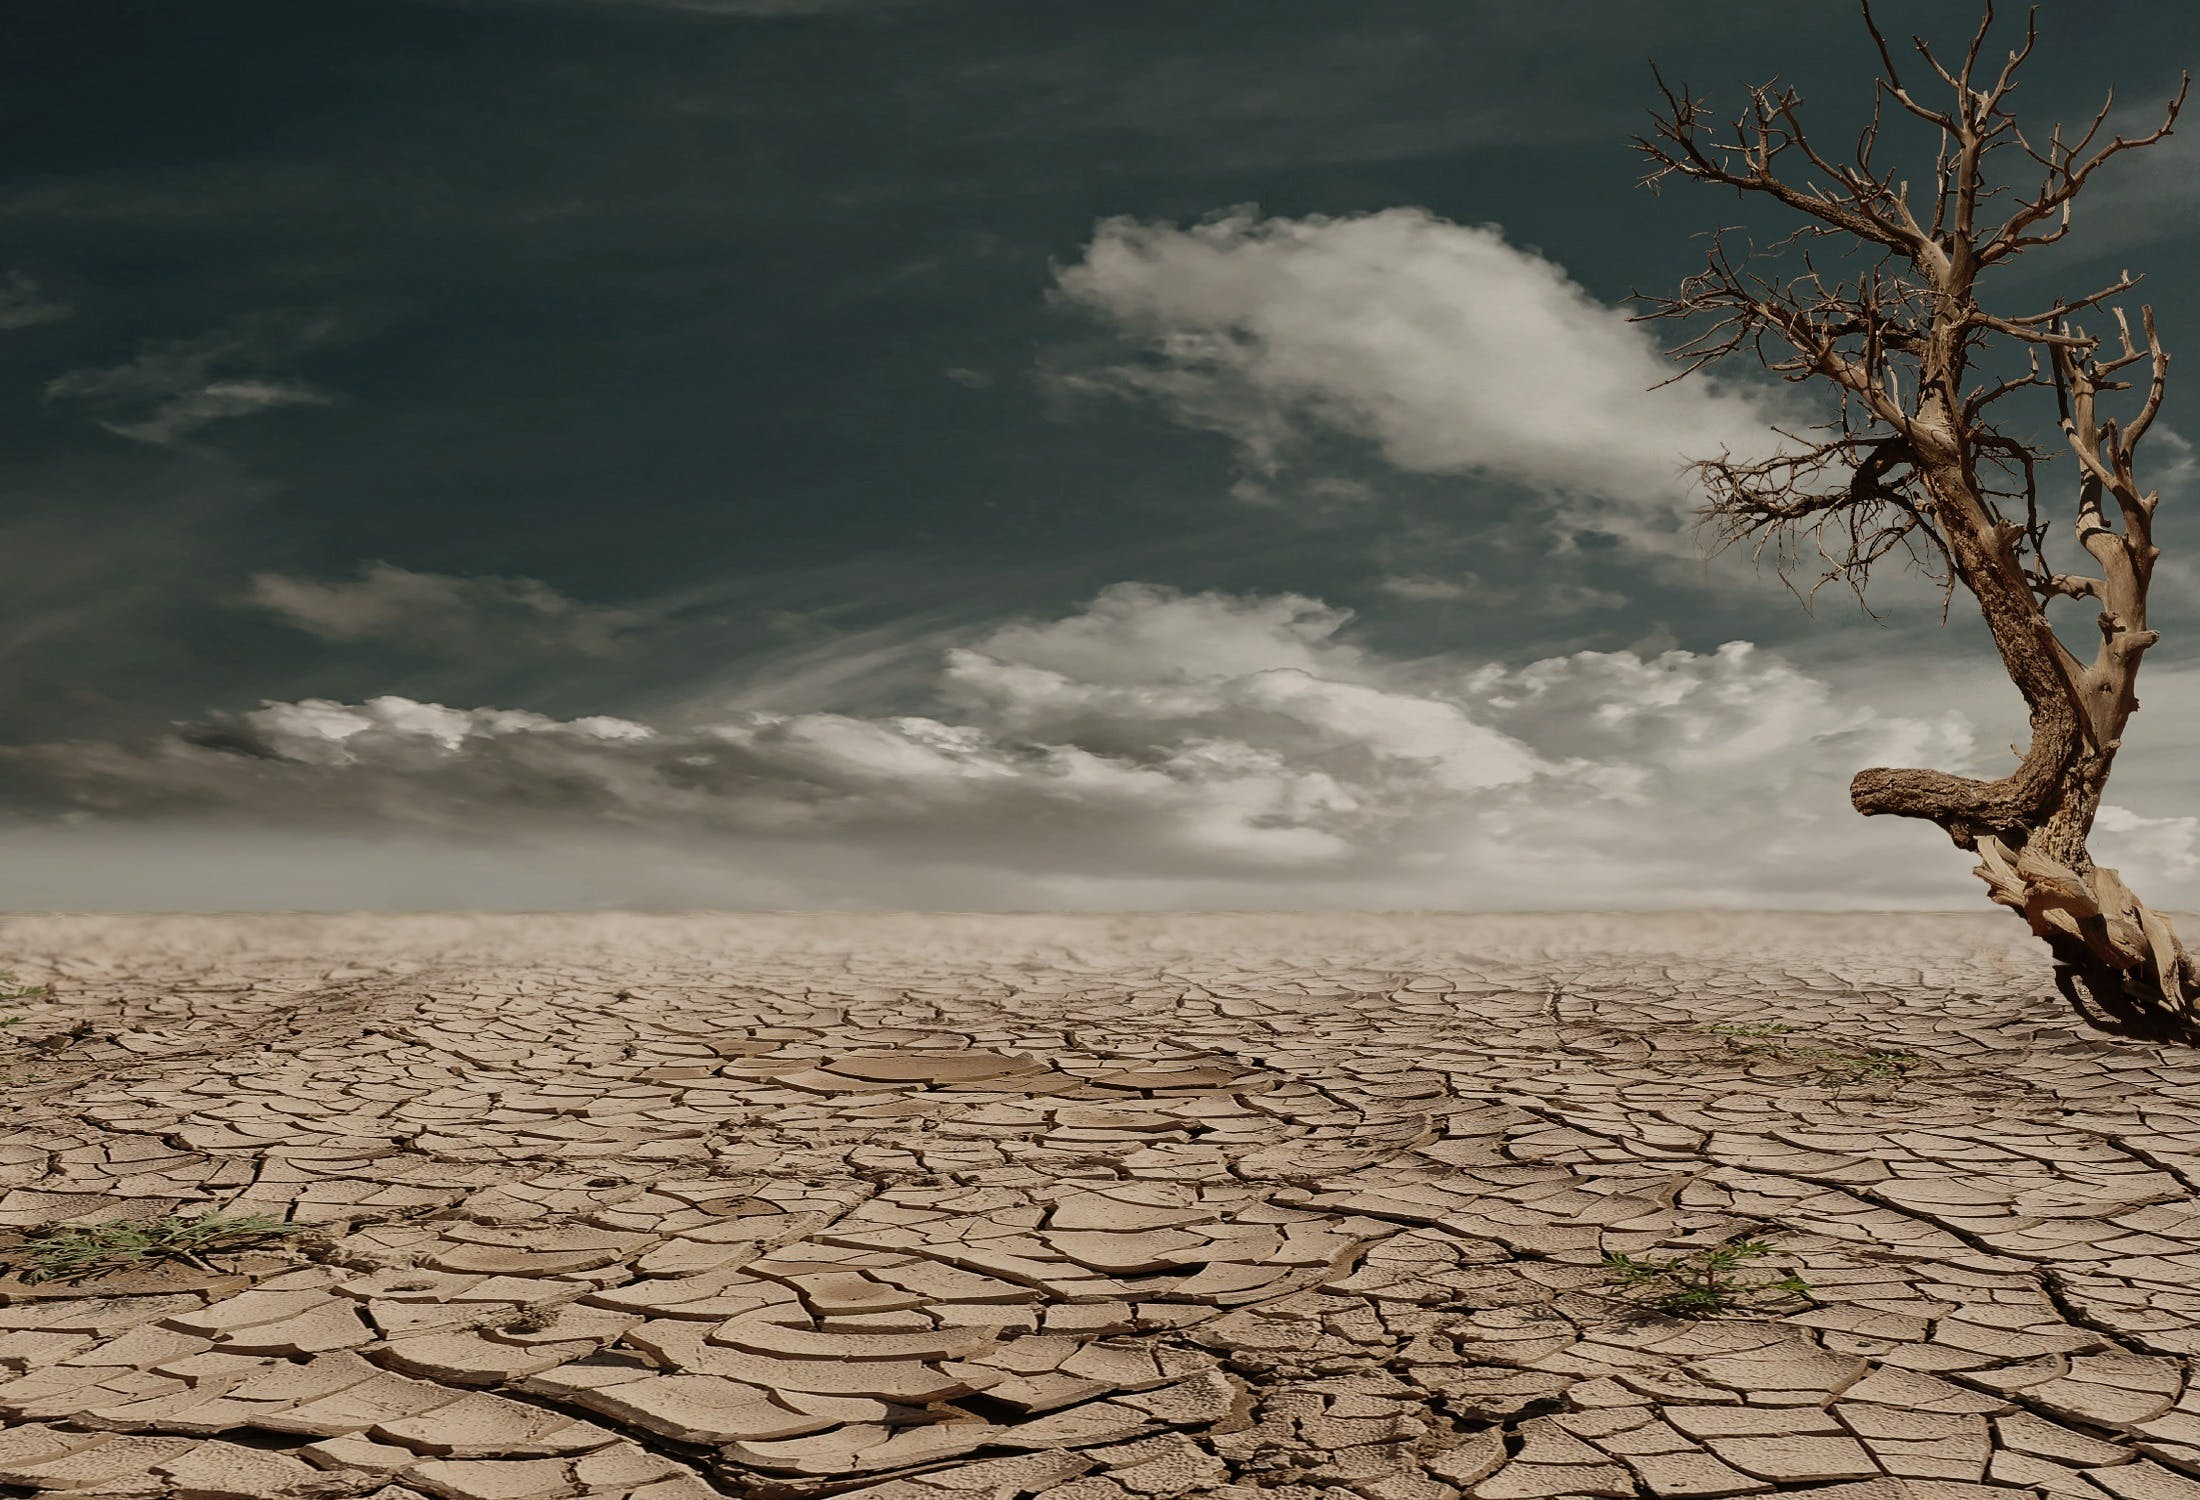
\includegraphics[width=0.75\linewidth]{cover} \end{center}

As the world faces the reality of climate change, natural hazards and extreme weather events have become a major concern, with devastating consequences for nature and humans. The quantification and definition of climate change, extreme events and its implications for life and health on our planet is one of the major concerns in climate science.

This book explains current statistical methods in climate science and their application.
We do not aim to provide a comprehensive overview of all statistical methods in climate science, but rather to give an overview of the most important methods and their application.
This book is the outcome of the seminar ``Climate and Statistics'' which took place in summer 2026 at the Department of Statistics, LMU Munich.

\begin{figure}
\centering
\pandocbounded{
\includegraphics[keepaspectratio,alt={Creative Commons License}]{book_files/by-nc-sa.png}}
\caption{Creative Commons License}
\end{figure}

This book is licensed under the \href{http://creativecommons.org/licenses/by-nc-sa/4.0/}{Creative Commons Attribution-NonCommercial-ShareAlike 4.0 International License}.

\mainmatter

\section*{Technical Setup}\label{technical-setup}


The book chapters are written in the Markdown language.
To combine R-code and Markdown, we used rmarkdown.
The book was compiled with the bookdown package.
We collaborated using git and github.
For details, head over to the \href{https://github.com/henrifnk/Seminar_ClimateNStatistics}{book's repository}.

\chapter{Melting Perspectives on Uncertainty in Climate}\label{unc}

\emph{Author: Shuangying Xu}

\emph{Supervisor: Henri Funk}

\emph{Degree: Bachelor}

\section{Abstract}\label{abstract}

Regional climate projections contain uncertainty from both internal variability and differences among climate-model responses, and these sources can affect how projected warming is interpreted. This seminar work examines fixed-scenario uncertainty in 20-year mean regional JJA warming across Northern Europe, Western and Central Europe, and the Mediterranean using five MMLEAv2 large-ensemble models with 166 ensemble members under SSP3-7.0. Internal variability is estimated from within-model member spread, while model uncertainty is estimated from differences among model-specific ensemble-mean responses using equal model weighting. The analysis further uses prediction ranges, signal-to-noise ratios, threshold exceedance probabilities, hierarchical bootstrap, and balanced-member sensitivity tests. Regional summer warming increases across the century in all three regions, while model-specific responses become increasingly separated. Internal variability in the 20-year warming target remains comparatively stable, whereas model uncertainty grows and becomes the dominant contributor to total fixed-scenario uncertainty. Projection ranges also widen with lead time, with Northern Europe showing particularly large spread despite lower central warming than the other regions. The warming signal is clear relative to internal variability, but disagreement among models reduces confidence in its exact magnitude. Robustness analyses support these qualitative patterns. Overall, the results show that uncertainty attribution depends not only on the model ensemble but also on the definition and temporal averaging of the prediction target.

\section{Introduction}\label{introduction}

Uncertainty is a central feature of climate projections and can arise from different sources, providing multiple perspectives on how future climate should be interpreted \citep{Hawkins2009}. Understanding these different dimensions of uncertainty is important because projected climate change cannot be fully described by a single expected value. This seminar work examines these issues in the context of projected regional summer temperature change.

\subsection{Background and Motivation: Uncertainty in Regional Climate Projections}\label{background-and-motivation-uncertainty-in-regional-climate-projections}

At regional scales, climate projections are better understood as a range of possible outcomes than as a single estimate of future change. Different simulations can follow different climate trajectories, while different climate models can also produce different responses to external forcing. Ensemble projections therefore provide information not only about the expected climate response, but also about the spread around that response \citep{Tebaldi2007, Hawkins2009}.

This spread is particularly relevant for regional climate change. The importance of different sources of uncertainty depends on the region, projection horizon, and spatial and temporal averaging scale \citep{Hawkins2009}. Natural climate variability is generally more visible at regional and shorter time scales and may temporarily strengthen or weaken the underlying climate-change signal \citep{Deser2020, Gruber2026}. Temporal averaging can reduce the influence of shorter-term fluctuations, so the magnitude of uncertainty also depends on how the projection target is defined \citep{Hawkins2009}.

Regional summer temperature is especially relevant for climate-impact assessment. In Europe, increasing temperature and extreme heat are associated with risks to human health, agricultural production, ecosystems, infrastructure, and energy demand, while the severity of these impacts differs across regions \citep{BednarFriedl2022}. Regional June--July--August (JJA) temperature therefore provides a useful indicator for examining both the magnitude of future warming and the uncertainty surrounding it.

A multi-model mean alone cannot fully describe these different perspectives on a projection. It does not show the variation among simulations, the disagreement among model responses, or the overall width of the projected warming distribution. A distribution-based interpretation can therefore complement the mean by describing both the magnitude and structure of projection uncertainty. These considerations motivate examining regional warming in terms of how large the projected change is, how uncertain it is, where that uncertainty comes from, and how the resulting distribution can be interpreted. To address these questions consistently, the next section introduces the statistical concepts of uncertainty and connects them to the structure of climate-model ensembles.

\subsection{Conceptual and Literature Framework}\label{conceptual-and-literature-framework}

The sources of projection uncertainty can be viewed through both statistical and climate-specific perspectives \citep{Gruber2025, Hawkins2009}. These perspectives are related, but their correspondence is interpretive rather than exact, especially when applied to complex climate-model ensembles. This section develops that connection and uses it to organize the large-ensemble, fixed-scenario, and distribution-based framework adopted in the analysis.

\subsubsection{Statistical Concepts of Uncertainty}\label{statistical-concepts-of-uncertainty}

A common statistical distinction is between aleatoric and epistemic uncertainty.

\textbf{Aleatoric uncertainty} refers to stochastic variation that remains under a given information set. In probabilistic terms, it can be represented by the conditional distribution of an outcome \(Y\) given available information \(X=x\), with its magnitude often summarized by the conditional variance,

\[
\operatorname{Var}(Y \mid X=x).
\]

If this conditional distribution is not concentrated at a single value, the outcome cannot be predicted exactly even when the underlying relationship is known \citep{Gruber2025}.

\textbf{Epistemic uncertainty}, in contrast, arises from incomplete knowledge about the process being represented. It may reflect imperfect model structure, missing information, omitted processes, or simplifying assumptions, and may in principle be reduced as knowledge, observations, or models improve \citep{Gruber2025}. The distinction between aleatoric and epistemic uncertainty is nevertheless context-dependent. Variation that appears irreducible under one information set may become partly explainable when additional information is available. The classification therefore depends on the model, the data, and the information being conditioned on.

The aleatoric--epistemic distinction is useful for organizing sources of uncertainty, but it does not imply that all sources can be separated cleanly or combined through a general additive decomposition \citep{Gruber2025}. More generally, uncertainty can be represented through probability distributions and summarized using measures such as variance, standard deviation, intervals, and probabilities. The following section relates these statistical concepts to the main uncertainty sources in climate projections.

\subsubsection{Climate-Specific Uncertainty and Its Statistical Interpretation}\label{climate-specific-uncertainty-and-its-statistical-interpretation}

Climate projections are commonly affected by three broad sources of uncertainty: internal variability, model uncertainty, and scenario uncertainty \citep{Hawkins2009}. These sources arise from different parts of the climate-projection process and can be related, with appropriate qualifications, to the statistical concepts introduced above.

\textbf{Internal variability} refers to fluctuations generated by the inherently chaotic dynamics of the climate system. Under the same model structure and external forcing, small differences in initial conditions can lead to different climate trajectories. In a single-model initial-condition large ensemble, the resulting spread among ensemble members therefore represents variability that remains when model structure and forcing are held fixed \citep{Gruber2026}. In this conditional sense, internal variability has an aleatoric-like interpretation because it represents stochastic variation within the modeled climate system. This interpretation is not exact, however, because it depends on how well the climate model represents the underlying stochastic dynamics of the real climate system \citep{Gruber2026}. The magnitude of this member-to-member variability also depends on the spatial and temporal scale of the climate quantity being analyzed \citep{Hawkins2009}.

\textbf{Model uncertainty} describes differences in the simulated forced response across climate models exposed to comparable external forcing \citep{Hawkins2009}. These differences may arise from model structure, parameterizations, representations of physical processes, and climate feedbacks. From a statistical perspective, model uncertainty has an epistemic-like interpretation because it reflects incomplete knowledge about how the climate system should be represented \citep{Gruber2025}. In a multi-model large ensemble, differences among model-specific responses can therefore provide an empirical representation of model uncertainty. However, the spread among a finite set of climate models should not be interpreted as the full epistemic uncertainty associated with the real climate system.

\textbf{Scenario uncertainty} arises from differences among possible future forcing pathways. Future emissions, land use, and other external drivers are not known in advance, and alternative pathways can therefore produce different climate responses \citep{Hawkins2009}. Unlike internal variability, scenario uncertainty does not describe stochastic variation among realizations under the same forcing. It is more appropriately interpreted as uncertainty associated with alternative conditioning pathways. Because the present analysis later conditions on a single forcing pathway, scenario uncertainty is outside the empirical decomposition considered in this study.

The relationship between statistical and climate-specific uncertainty can therefore be summarized as follows:

\begin{longtable}[]{@{}
  >{\raggedright\arraybackslash}p{(\linewidth - 4\tabcolsep) * \real{0.3194}}
  >{\raggedright\arraybackslash}p{(\linewidth - 4\tabcolsep) * \real{0.3194}}
  >{\raggedright\arraybackslash}p{(\linewidth - 4\tabcolsep) * \real{0.3611}}@{}}
\caption{\label{tab:unc-uncertainty-category} Conceptual relationship between climate-specific and statistical uncertainty.}\tabularnewline
\toprule\noalign{}
\begin{minipage}[b]{\linewidth}\raggedright
Climate uncertainty source
\end{minipage} & \begin{minipage}[b]{\linewidth}\raggedright
Statistical interpretation
\end{minipage} & \begin{minipage}[b]{\linewidth}\raggedright
Role in this study
\end{minipage} \\
\midrule\noalign{}
\endfirsthead
\toprule\noalign{}
\begin{minipage}[b]{\linewidth}\raggedright
Climate uncertainty source
\end{minipage} & \begin{minipage}[b]{\linewidth}\raggedright
Statistical interpretation
\end{minipage} & \begin{minipage}[b]{\linewidth}\raggedright
Role in this study
\end{minipage} \\
\midrule\noalign{}
\endhead
\bottomrule\noalign{}
\endlastfoot
Internal variability & Aleatoric-like & Within-model member variation \\
Model uncertainty & Epistemic-like & Spread among model responses \\
Scenario uncertainty & Conditional pathway & Held fixed in the analysis \\
\end{longtable}

These correspondences provide a useful framework for organizing the analysis, but they should not be treated as strict identities. Whether a source is interpreted as aleatoric or epistemic depends on the model, available information, and conditioning assumptions \citep{Gruber2025}. The next section translates these concepts into the hierarchical structure of multi-model large ensembles and defines the climate quantity to which the uncertainty is attached.

\subsubsection{Hierarchical Large-Ensemble Framework}\label{hierarchical-large-ensemble-framework}

The structure of a multi-model large ensemble provides a natural way to distinguish within-model from between-model variation. For regional summer warming, this structure can be represented conceptually as

\begin{equation}
Y_{m,r,R,P}
=
\mu_{R,P}
+
a_{m,R,P}
+
\varepsilon_{m,r,R,P},
\label{eq:unc-hierarchical-framework}
\end{equation}

where \(Y_{m,r,R,P}\) denotes period-mean regional JJA warming for model \(m\), ensemble member \(r\), region \(R\), and future period \(P\). The term \(\mu_{R,P}\) represents the multi-model mean forced response, \(a_{m,R,P}\) represents the model-specific deviation from this mean, and \(\varepsilon_{m,r,R,P}\) represents the member-specific deviation associated with internal variability. Equation \eqref{eq:unc-hierarchical-framework} therefore separates variation across model responses from variation among members of the same model.

Within a single-model initial-condition large ensemble, members share the same model formulation and external forcing but follow different trajectories because of small differences in initial conditions. Member-to-member variation can therefore be used to characterize internal variability, while averaging across members reduces the influence of individual internal fluctuations and provides an estimate of the model-specific forced response \citep{Gruber2026, Deser2020}. Because the ensemble is finite, the ensemble mean remains an estimate rather than the exact forced response.

Extending this structure across several climate models introduces a second level of variation. Differences among model-specific ensemble means represent differences in simulated forced responses, while variation around each model mean represents within-model internal variability. Multiple large ensembles therefore separate these two levels more clearly than collections of single realizations, where internal fluctuations and differences in forced responses can be difficult to distinguish \citep{Lehner2020}.

Because the models contain different numbers of ensemble members, model-level and member-level information should be treated separately rather than pooling all members with equal influence across models. The equal-model weighting design is described in Section 2.4, while the corresponding estimators are introduced in the Methods section.

\subsubsection{Fixed-Scenario and Distributional Interpretation}\label{fixed-scenario-and-distributional-interpretation}

When the analysis is conditioned on a single future forcing pathway, differences among alternative scenarios fall outside the quantities being estimated. The resulting uncertainty should therefore be interpreted as conditional on that pathway rather than as the complete uncertainty associated with future climate projections \citep{Hawkins2009}.

Within this conditional setting, the analysis focuses on two sources of variation identified above: internal variability within climate models and differences in forced responses across models. The variance decomposition used later provides an operational way to quantify the magnitude and relative contribution of these components. It is specific to the climate-ensemble framework adopted in this study and should not be interpreted as a general additive decomposition of aleatoric and epistemic uncertainty.

Variance decomposition alone, however, does not fully describe the projected warming distribution. A distributional perspective complements source-based decomposition by considering both the location and spread of possible warming outcomes \citep{Tebaldi2007}. Prediction ranges describe the absolute spread of the distribution, signal-to-noise ratios compare the warming signal with uncertainty, and threshold exceedance probabilities describe the position of the distribution relative to specified warming levels \citep{Hawkins2009}.

These diagnostics provide complementary views of the same regional warming distribution: how uncertain it is, how clearly the warming signal emerges relative to that uncertainty, and where the projected outcomes lie relative to selected thresholds. Their specific definitions and estimators are introduced in the Methods section.

\subsection{Study Aim and Research Questions}\label{study-aim-and-research-questions}

Building on the conceptual framework above, this section defines the focus of the seminar work and translates it into research questions on regional summer warming and its uncertainty.

\textbf{Study Aim}

This seminar work aims to quantify, decompose, and interpret fixed-scenario uncertainty in projected regional JJA temperature change across selected European IPCC AR6 reference regions. The study applies established large-ensemble methods to distinguish internal variability from differences among model responses and to interpret the resulting warming distribution.

\textbf{Study Scope}

The study uses monthly near-surface air temperature (\texttt{tas}) from five CMIP6 large-ensemble models in MMLEAv2, comprising 166 ensemble members under SSP370. The analysis covers Northern Europe (NEU), Western and Central Europe (WCE), and the Mediterranean (MED), with warming calculated relative to the 1995--2014 baseline for three 20-year future periods: 2021--2040, 2041--2060, and 2081--2100. The analysis focuses on internal variability and model uncertainty and complements their decomposition with prediction ranges, internal and total signal-to-noise ratios, and exceedance probabilities for \(2^\circ\mathrm{C}\) and \(3^\circ\mathrm{C}\) warming.

\textbf{Research Questions}

The study is guided by three research questions:

\textbf{RQ1: Warming magnitude.} How much does regional JJA temperature increase relative to the 1995--2014 baseline across the selected regions and future periods?

\textbf{RQ2: Uncertainty magnitude and source.} How large are internal variability, model uncertainty, and total fixed-scenario projection uncertainty in 20-year mean warming, and how do their relative contributions vary across regions and periods?

\textbf{RQ3: Interpretation of projection uncertainty.} How can the projected regional warming distribution be interpreted through prediction ranges, signal-to-noise ratios, and threshold exceedance probabilities?

\textbf{Analytical Approach}

The analysis follows a consistent workflow from climate-model output to uncertainty interpretation. Monthly gridded \texttt{tas} is first aggregated to regional annual JJA temperature and then expressed as future-period warming relative to the 1995--2014 baseline. Ensemble information is used to distinguish model-specific forced responses, within-model internal variability, and between-model differences in forced responses. Multi-model quantities are constructed with equal model influence, while the resulting warming distribution is interpreted using prediction ranges, signal-to-noise ratios, and threshold exceedance probabilities. Robustness is assessed through hierarchical bootstrap and balanced 20-member subsampling.

\section{Data and Study Design}\label{data-and-study-design}

This chapter describes the data and study design used to define the regional climate projections analyzed in this work. It introduces the ensemble dataset, model and member selection, spatial and temporal domains, and the conditioning and weighting choices that determine the scope of the subsequent uncertainty analysis.

\subsection{MMLEAv2 Dataset and Climate Variable}\label{mmleav2-dataset-and-climate-variable}

The analysis uses the Multi-Model Large Ensemble Archive Version 2 (MMLEAv2), an updated collection of initial-condition large ensembles designed to facilitate comparison across climate models \citep{Maher2025}. The archive contains multiple climate models and ensemble members on a common \(2.5^\circ \times 2.5^\circ\) horizontal grid and provides a range of monthly climate variables \citep{Maher2025}. The variable used in this study is monthly near-surface air temperature (\texttt{tas}).

For the selected model ensemble, historical simulations are used to establish the reference-period climate, while SSP370 simulations provide the data for the future periods. The original gridded data are organized hierarchically by climate model, ensemble member, year, month, and grid cell. This structure preserves both repeated realizations within individual models and differences across models.

MMLEAv2 is therefore well suited to the uncertainty framework developed in Section 1.2. Multiple members within the same model provide information on within-model variability, whereas the availability of multiple large ensembles allows differences among model responses to be examined \citep{Maher2025}. The statistical inference in this study is conditional on the selected subset of MMLEAv2 models and simulations, which is described in the following section.

\subsection{Model and Ensemble-Member Selection}\label{model-and-ensemble-member-selection}

Five CMIP6 large ensembles from MMLEAv2 were selected for the main analysis, giving a total of 166 ensemble members. The selected models and ensemble sizes are summarized in Table \ref{tab:unc-model-members}.

\begin{longtable}[]{@{}ll@{}}
\caption{\label{tab:unc-model-members} Selected climate models and ensemble-member counts used in the main analysis.}\tabularnewline
\toprule\noalign{}
Model & Members used \\
\midrule\noalign{}
\endfirsthead
\toprule\noalign{}
Model & Members used \\
\midrule\noalign{}
\endhead
\bottomrule\noalign{}
\endlastfoot
ACCESS-ESM1-5 & 40 \\
CanESM5 & 25 \\
CESM2 (CMIP6) & 50 \\
E3SMv2 & 21 \\
MPI-ESM1-2-LR & 30 \\
\end{longtable}

Thus,

\[
M=5,
\qquad
N=166.
\]

Member selection was based on the availability of the historical and SSP370 simulations required for the analysis, with additional consistency rules for CESM2 and CanESM5. For CESM2, the large ensemble contains two groups of 50 members that differ in their treatment of biomass-burning forcing. The present study uses the 50 members following the original CMIP6 biomass-burning forcing protocol, thereby avoiding the combination of the two forcing configurations within a single model ensemble \citep{Rodgers2021}. For CanESM5, one consistent group of 25 \texttt{p1} members is used. The \texttt{p1} and \texttt{p2} ensembles differ in the remapping of wind-stress fields, so restricting the analysis to one variant avoids treating this configuration difference as internal variability \citep{Swart2019}. For ACCESS-ESM1-5, E3SMv2, and MPI-ESM1-2-LR, the available members with the required historical and SSP370 data are retained.

The ensemble sizes therefore differ considerably across models. Directly pooling all 166 members with equal member weight would give greater influence to models with larger ensembles, particularly CESM2 and ACCESS-ESM1-5. Multi-model quantities are instead constructed so that each climate model receives the same total analytical weight. The formal weighting scheme is described in Section 2.4.

\subsection{Study Regions and Time Periods}\label{study-regions-and-time-periods}

The analysis focuses on three European reference regions from the IPCC AR6 regional framework: Northern Europe (NEU), Western and Central Europe (WCE), and the Mediterranean (MED) \citep{Iturbide2020}. These standardized regions provide a consistent basis for comparing regional climate-model output and allow differences in projected warming and uncertainty to be examined across northern, central, and southern Europe. The spatial extent of the three study regions is shown in Figure \ref{fig:unc-study-region-map}.

\begin{figure}

{\centering 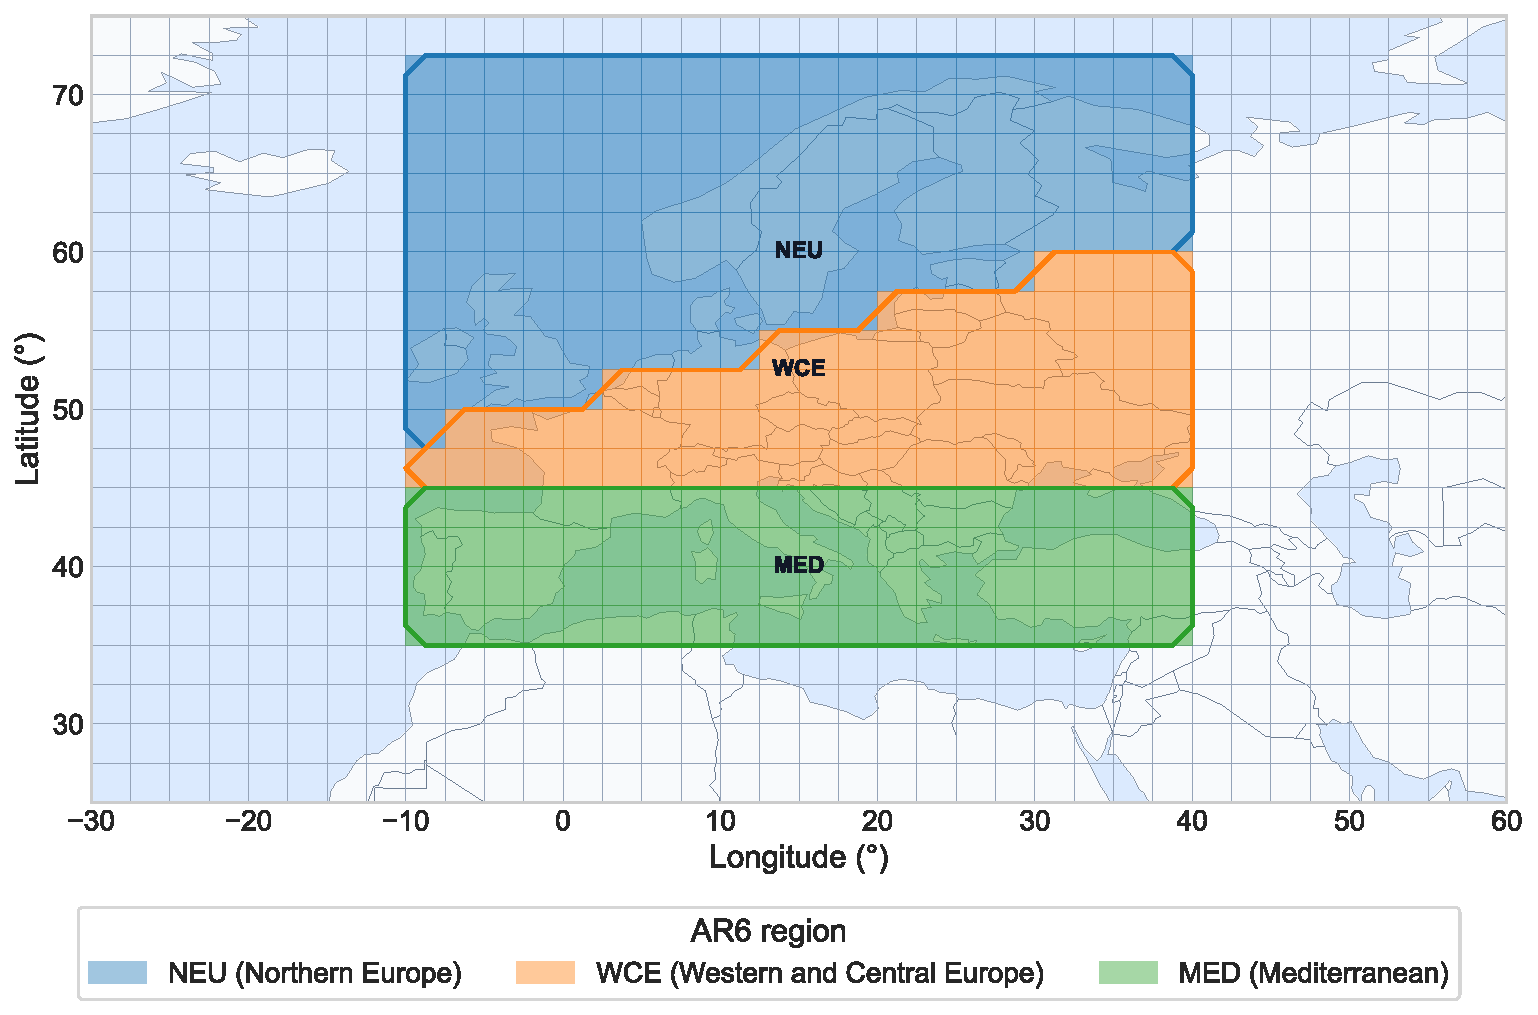
\includegraphics[width=1\linewidth]{work/01-climate_uncertainty/figures/fig01_study_region_map} 

}

\caption{Study regions used in the analysis: NEU, WCE, and MED.}\label{fig:unc-study-region-map}
\end{figure}

The baseline period is defined as

\[
P_0 = 1995\text{--}2014.
\]

Projected warming is evaluated for three 20-year future periods,

\[
P_1 = 2021\text{--}2040,
\qquad
P_2 = 2041\text{--}2060,
\qquad
P_3 = 2081\text{--}2100.
\]

These periods represent the near-term, mid-term, and late-century projection windows used in this study and are consistent with the time-slice framework used in the IPCC AR6 assessment \citep{IPCC2021}. All temperature changes are calculated relative to the 1995--2014 baseline.

The \(2^\circ\mathrm{C}\) and \(3^\circ\mathrm{C}\) thresholds considered later in the analysis refer specifically to regional JJA warming relative to 1995--2014. They should therefore not be interpreted as global warming levels relative to the pre-industrial period.

\subsection{Fixed-Scenario Design and Equal Model Weighting}\label{fixed-scenario-design-and-equal-model-weighting}

All future simulations in this study follow the SSP3-7.0 forcing pathway, identified as \texttt{ssp370} in CMIP6. SSP3-7.0 is part of the ScenarioMIP design for CMIP6 and represents a relatively high-forcing future pathway \citep{ONeill2016}. Because only one forcing pathway is considered, differences among alternative future scenarios are not sampled in the present analysis. Scenario uncertainty is therefore outside the uncertainty decomposition used in this study \citep{Hawkins2009}.

The resulting uncertainty estimates are interpreted as \textbf{total fixed-scenario projection uncertainty}. They describe uncertainty associated with internal variability and differences among the selected model responses under the same forcing pathway, rather than the full uncertainty across alternative future scenarios. The formal variance decomposition is introduced later in the Methods section.

Because the five models contain different numbers of ensemble members, the analysis gives each model equal total influence in multi-model summaries rather than pooling all members with equal weight across models. Model-level information is therefore combined using equal model weighting, while members within each model contribute within that model's share. This prevents models with larger ensembles from receiving greater influence solely because they contain more members, but it does not imply that the five models are equally accurate \citep{Tebaldi2007}.

The resulting inference is conditional on the SSP3-7.0 pathway, the five selected climate models, JJA temperature, and the three European study regions. Together with the spatial and temporal domains defined above, these conditions specify the scope within which the subsequent uncertainty estimates and distributional diagnostics are interpreted.

\section{Methods}\label{methods}

Building on the data and study design described above, this chapter defines the statistical procedures used to construct the regional JJA warming indicator and quantify its uncertainty. The analysis proceeds from temperature aggregation and warming calculation to forced-response estimation, uncertainty decomposition, distribution-based diagnostics, and robustness assessment.

\subsection{Analytical Framework and Statistical Targets}\label{analytical-framework-and-statistical-targets}

The analysis is organized around the hierarchical structure of the multi-model large ensemble. Let \(m\) denote the climate model, \(r\) the ensemble member, \(R\) the study region, and \(P\) the future period. The indices \(y\) and \(g\) are used below for year and grid cell, respectively.

The core response variable is

\[
Y_{m,r,R,P},
\]

which represents the 20-year mean regional JJA warming for model \(m\), member \(r\), region \(R\), and period \(P\), relative to the 1995--2014 baseline. The detailed construction of this quantity from monthly gridded \texttt{tas} is given in Section 3.2. Importantly, the uncertainty analyzed below therefore concerns member-to-member variation in 20-year mean warming rather than year-to-year JJA temperature variability.

The main statistical targets are the model-specific forced response \(\overline{Y}_{m,R,P}\), the equal-model-weighted multi-model response \(\overline{Y}_{\cdot,R,P}\), and the internal, model, and total fixed-scenario uncertainty components \(U_{\mathrm{internal},R,P}\), \(U_{\mathrm{model},R,P}\), and \(U_{\mathrm{total},R,P}\). Their relative contributions are evaluated using variance contribution rates. The same model-member warming values are then used to characterize the projection distribution through prediction quantiles, signal-to-noise ratios, and threshold exceedance probabilities.

The overall analytical workflow is summarized in Figure \ref{fig:unc-workflow}.

\begin{figure}

{\centering 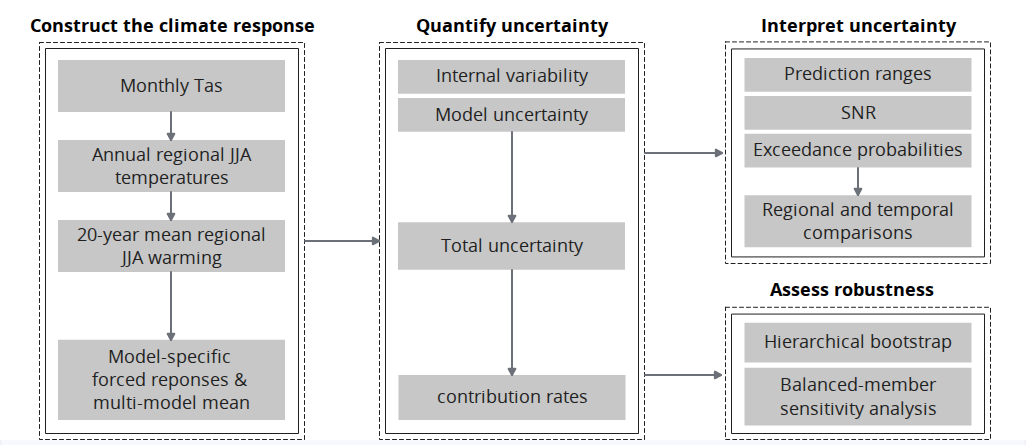
\includegraphics[width=1\linewidth]{work/01-climate_uncertainty/figures/workflow} 

}

\caption{Analytical Sequence}\label{fig:unc-workflow}
\end{figure}

\subsection{Construction of the Regional Summer Warming Indicator}\label{construction-of-the-regional-summer-warming-indicator}

The core response variable is constructed from monthly gridded \texttt{tas} in two stages. First, monthly temperature is aggregated to annual regional JJA mean temperature using seasonal and spatial weighting; second, temperature anomalies relative to the 1995--2014 baseline are averaged over each 20-year future period. These steps produce a consistent regional warming indicator for each model and ensemble member.

\subsubsection{JJA and Spatial Aggregation}\label{jja-and-spatial-aggregation}

Monthly \texttt{tas} values were first converted from kelvin to degrees Celsius where necessary,

\[
T(^\circ\mathrm{C})
=
T(\mathrm{K})-273.15.
\]

Because temperature differences have the same numerical magnitude in kelvin and degrees Celsius, this conversion does not affect the later warming anomalies.

For each model, ensemble member, year, and grid cell, summer temperature was calculated from June, July, and August using the number of days in each month. Under the JJA weighting used in this analysis,

\[
T^{\mathrm{JJA}}_{m,r,y,g}
=
\frac{
30T_{m,r,y,6,g}
+
31T_{m,r,y,7,g}
+
31T_{m,r,y,8,g}
}{92},
\]

where \(T_{m,r,y,k,g}\) denotes the monthly mean temperature for month \(k\) at grid cell \(g\).

The gridded JJA values were then aggregated to the study regions using cosine-latitude weights. For grid cell \(g\) in region \(R\), the normalized spatial weight is

\[
w_g
=
\frac{\cos(\phi_g)}
{\sum_{h\in R}\cos(\phi_h)},
\]

where \(\phi_g\) is the latitude of the grid-cell center and the weights satisfy

\[
\sum_{g\in R} w_g = 1.
\]

The annual regional JJA mean temperature is therefore

\[
I_{m,r,y,R}
=
\sum_{g\in R}
w_g T^{\mathrm{JJA}}_{m,r,y,g}.
\]

This procedure produces one regional JJA mean temperature for each model, ensemble member, year, and study region. These annual regional values are used in the next step to calculate baseline-relative anomalies and 20-year period-mean warming.

\subsubsection{Baseline Anomalies and Period Means}\label{baseline-anomalies-and-period-means}

For each model, ensemble member, and region, the reference climate is defined as the mean regional JJA temperature over the 1995--2014 baseline period \(P_0\),

\[
I_{m,r,P_0,R}
=
\frac{1}{|P_0|}
\sum_{y\in P_0}
I_{m,r,y,R},
\]

where \(|P_0|=20\). Calculating the baseline separately for each model and ensemble member allows the analysis to focus on simulated temperature change rather than differences in absolute climatology.

Annual JJA temperature anomalies are then calculated relative to the corresponding baseline,

\[
\Delta I_{m,r,y,R}
=
I_{m,r,y,R}
-
I_{m,r,P_0,R}.
\]

For each future period \(P\), the core response variable is defined as the mean anomaly over the 20 years in that period:

\begin{equation}
Y_{m,r,R,P}
=
\frac{1}{|P|}
\sum_{y\in P}
\Delta I_{m,r,y,R},
\qquad |P|=20.
\label{eq:unc-period-mean-warming}
\end{equation}

Thus, \(Y_{m,r,R,P}\) represents the 20-year mean regional JJA warming for one model and ensemble member relative to 1995--2014. All subsequent forced-response estimates, uncertainty components, and distributional diagnostics are calculated from these period-mean warming values.

\subsection{Estimation of Forced Responses and Uncertainty Components}\label{estimation-of-forced-responses-and-uncertainty-components}

Using the 20-year mean warming values \(Y_{m,r,R,P}\), the analysis next separates the projected response into model-specific forced responses and uncertainty components. Ensemble means are used to estimate forced warming, while within-model member variation and between-model differences are used to quantify internal variability and model uncertainty. These components are then combined to characterize total fixed-scenario uncertainty and their relative contributions.

\subsubsection{Model-Specific and Multi-Model Forced Responses}\label{model-specific-and-multi-model-forced-responses}

For each climate model, the model-specific forced response is estimated by averaging the 20-year mean warming values across its ensemble members,

\begin{equation}
\overline{Y}_{m,R,P}
=
\frac{1}{n_m}
\sum_{r=1}^{n_m}
Y_{m,r,R,P},
\label{eq:unc-model-forced-response}
\end{equation}

where (n\_m) is the number of ensemble members available for model (m). Because members of the same model share the same model formulation and external forcing, averaging across members reduces the influence of member-specific internal fluctuations. The resulting ensemble mean is therefore interpreted as an estimate of that model's forced warming response \citep{Deser2020, Lehner2020}. Internal variability is not assumed to be completely removed, because the ensemble contains a finite number of members.

The multi-model mean forced response is then calculated from the model-specific ensemble means,

\begin{equation}
\overline{Y}_{\cdot,R,P}
=
\frac{1}{M}
\sum_{m=1}^{M}
\overline{Y}_{m,R,P},
\label{eq:unc-multimodel-forced-response}
\end{equation}

where (M=5) is the number of climate models. Equation \eqref{eq:unc-multimodel-forced-response} gives each model the same total weight, regardless of its ensemble size. The calculation therefore averages within models first and then across models, rather than pooling all 166 ensemble members with equal weight.

The resulting multi-model mean provides an equal-model-weighted summary of the forced warming responses represented by the selected models. Differences between the individual model-specific responses and this multi-model mean form the basis for estimating between-model uncertainty in the following section.

\subsubsection{Within-Model and Between-Model Variance}\label{within-model-and-between-model-variance}

Internal variability is estimated from the spread of ensemble members around the model-specific forced response. For each model, region, and future period, the within-model variance is calculated as

\begin{equation}
s^2_{\mathrm{internal},m,R,P}
=
\frac{1}{n_m-1}
\sum_{r=1}^{n_m}
\left(
Y_{m,r,R,P}
-
\overline{Y}_{m,R,P}
\right)^2.
\label{eq:unc-within-model-variance}
\end{equation}

Because \(Y_{m,r,R,P}\) represents 20-year mean warming, Equation \eqref{eq:unc-within-model-variance} measures member-to-member variability in the 20-year warming response within model \(m\), rather than year-to-year temperature variability. This within-model spread provides the operational measure of internal variability used in the analysis \citep{Deser2020, Lehner2020}.

To prevent models with larger ensembles from contributing more strongly to the multi-model estimate, the model-specific variances are averaged with equal model weight,

\begin{equation}
U_{\mathrm{internal},R,P}
=
\frac{1}{M}
\sum_{m=1}^{M}
s^2_{\mathrm{internal},m,R,P}.
\label{eq:unc-internal-variance}
\end{equation}

The corresponding internal standard deviation is

\[
\sigma_{\mathrm{internal},R,P}
=
\sqrt{U_{\mathrm{internal},R,P}}.
\]

Model uncertainty is estimated at the second level of the ensemble hierarchy. It is defined from the spread of the model-specific forced-response estimates around the equal-model-weighted multi-model mean,

\begin{equation}
U_{\mathrm{model},R,P}
=
\frac{1}{M-1}
\sum_{m=1}^{M}
\left(
\overline{Y}_{m,R,P}
-
\overline{Y}_{\cdot,R,P}
\right)^2.
\label{eq:unc-model-variance}
\end{equation}

with the corresponding standard deviation

\[
\sigma_{\mathrm{model},R,P}
=
\sqrt{U_{\mathrm{model},R,P}}.
\]

The two quantities therefore describe different levels of variation in the ensemble: \(U_{\mathrm{internal},R,P}\) summarizes within-model member variation, whereas \(U_{\mathrm{model},R,P}\) summarizes differences among the forced responses of the selected models. Variances are retained for the subsequent uncertainty decomposition, while the corresponding standard deviations express uncertainty magnitude in the same temperature units as the warming response.

\subsubsection{Total Uncertainty and Contribution Rates}\label{total-uncertainty-and-contribution-rates}

Under the fixed-scenario framework, total projection uncertainty is defined as the sum of the internal and model variance components,

\begin{equation}
U_{\mathrm{total},R,P}
=
U_{\mathrm{internal},R,P}
+
U_{\mathrm{model},R,P}.
\label{eq:unc-total-variance}
\end{equation}

This quantity represents the total variance considered in the present analysis and is therefore conditional on the SSP3-7.0 pathway and the selected climate-model ensemble. The corresponding total standard deviation is

\begin{equation}
\sigma_{\mathrm{total},R,P}
=
\sqrt{
U_{\mathrm{internal},R,P}
+
U_{\mathrm{model},R,P}
}.
\label{eq:unc-total-standard-deviation}
\end{equation}

Thus, the two variance components are added before taking the square root. Internal and model standard deviations are not added directly.

To describe the relative importance of the two uncertainty sources, their contributions to total variance are calculated as

\begin{equation}
C_{\mathrm{internal},R,P}
=
\frac{
U_{\mathrm{internal},R,P}
}{
U_{\mathrm{total},R,P}
}.
\label{eq:unc-internal-contribution}
\end{equation}

and

\begin{equation}
C_{\mathrm{model},R,P}
=
\frac{
U_{\mathrm{model},R,P}
}{
U_{\mathrm{total},R,P}
}.
\label{eq:unc-model-contribution}
\end{equation}

By construction,

\[
C_{\mathrm{internal},R,P}
+
C_{\mathrm{model},R,P}
=
1.
\]

The contribution rates are relative measures and therefore depend on both variance components. A change in the internal contribution, for example, does not necessarily imply a corresponding change in the absolute magnitude of internal variability. The variance decomposition describes the magnitude and source of fixed-scenario uncertainty; the following section complements it with distribution-based measures of projection spread and interpretation.

\subsection{Distribution-Based Interpretation of Projection Uncertainty}\label{distribution-based-interpretation-of-projection-uncertainty}

Variance decomposition describes the magnitude and sources of projection uncertainty, but it does not fully characterize the distribution of possible warming outcomes. The analysis therefore complements the variance-based measures with prediction ranges, signal-to-noise ratios, and threshold exceedance probabilities, which describe the distributional spread, the clarity of the warming signal, and the position of projected warming relative to specified thresholds.

\subsubsection{Equal-Model-Weighted Prediction Ranges}\label{equal-model-weighted-prediction-ranges}

To describe the distribution of projected warming directly, the model-member warming values are combined into an equal-model-weighted empirical distribution. For region \(R\) and future period \(P\), the empirical cumulative distribution function is defined as

\begin{equation}
F_{R,P}(y)
=
\frac{1}{M}
\sum_{m=1}^{M}
\frac{1}{n_m}
\sum_{r=1}^{n_m}
\mathbf{1}
\left(
Y_{m,r,R,P}\le y
\right),
\label{eq:unc-empirical-mixture}
\end{equation}

where \(\mathbf{1}(\cdot)\) is the indicator function. This construction assigns each model a total weight of \(1/M\), while the members within model \(m\) share that weight equally. It therefore preserves equal model influence despite differences in ensemble size.

Weighted quantiles are obtained from Equation \eqref{eq:unc-empirical-mixture} as

\[
Q_{q,R,P}
=
F^{-1}_{R,P}(q),
\qquad
q\in\{0.05,0.50,0.95\}.
\]

Here, \(Q_{0.50,R,P}\) is the weighted median, while the 5th and 95th percentiles define the central 90\% prediction range,

\[
\mathrm{PI}_{90,R,P}
=
\left[
Q_{0.05,R,P},
Q_{0.95,R,P}
\right].
\]

The width of this range is

\[
W_{90,R,P}
=
Q_{0.95,R,P}
-
Q_{0.05,R,P}.
\]

Because the empirical distribution contains members from all selected models, the prediction range reflects both within-model member variation and differences among model responses. The range and its width are expressed directly in degrees Celsius and provide an absolute measure of projection spread. They are interpreted as descriptive ensemble-based ranges conditional on SSP3-7.0 and the selected model ensemble, rather than as confidence intervals for an unknown population parameter \citep{Tebaldi2007}.

\subsubsection{Signal-to-Noise Ratios}\label{signal-to-noise-ratios}

Signal-to-noise ratios are used to compare the magnitude of projected warming with the uncertainty surrounding that response. For each region and future period, the signal is defined as the absolute equal-model-weighted multi-model mean warming,

\[
\mathrm{Signal}_{R,P}
=
\left|
\overline{Y}_{\cdot,R,P}
\right|.
\]

Two noise scales are considered. The internal signal-to-noise ratio compares the warming signal with the standard deviation associated with within-model internal variability,

\begin{equation}
\mathrm{SNR}^{\mathrm{internal}}_{R,P}
=
\frac{
\left|
\overline{Y}_{\cdot,R,P}
\right|
}{
\sigma_{\mathrm{internal},R,P}
}.
\label{eq:unc-internal-snr}
\end{equation}

Equation \eqref{eq:unc-internal-snr} therefore measures how large the projected 20-year mean warming is relative to member-to-member variability within the climate models. A larger value indicates that the warming signal is more clearly separated from this internal variability.

The total signal-to-noise ratio additionally incorporates differences among model forced responses by using the total fixed-scenario standard deviation,

\begin{equation}
\mathrm{SNR}^{\mathrm{total}}_{R,P}
=
\frac{
\left|
\overline{Y}_{\cdot,R,P}
\right|
}{
\sigma_{\mathrm{total},R,P}
}.
\label{eq:unc-total-snr}
\end{equation}

Equation \eqref{eq:unc-total-snr} measures signal clarity relative to the combined internal and model uncertainty considered in this study. Comparing the two ratios therefore distinguishes signal clarity relative to internal variability from signal clarity after between-model disagreement is also included.

The ratios are interpreted descriptively: values below one indicate that the selected uncertainty scale is larger than the signal, values near one indicate similar magnitudes, and values above one indicate that the signal is larger than the selected uncertainty scale. An SNR greater than one is not a formal significance criterion or hypothesis test.

The definitions used here are standard-deviation-based SNR measures, consistent with large-ensemble applications that compare the magnitude of an ensemble-mean signal with ensemble spread \citep{McKinnon2018, McKinnon2021}. They differ from the 90\%-uncertainty scaling used in the SNR formulation of Hawkins and Sutton, so numerical SNR values should be interpreted according to the definition applied here \citep{Hawkins2009}.

\subsubsection{Threshold Exceedance Probabilities}\label{threshold-exceedance-probabilities}

Threshold exceedance probabilities are used to describe the position of the projected warming distribution relative to selected warming levels. The thresholds considered in this analysis are

\[
\theta
\in
\left\{
2^\circ\mathrm{C},
3^\circ\mathrm{C}
\right\}.
\]

As defined in Section 2.3, these thresholds refer to 20-year mean regional JJA warming relative to the 1995--2014 baseline.

For each model, the exceedance probability is estimated as the proportion of ensemble members whose period-mean warming exceeds threshold \(\theta\),

\begin{equation}
p_{m,R,P}(\theta)
=
\frac{1}{n_m}
\sum_{r=1}^{n_m}
\mathbf{1}
\left(
Y_{m,r,R,P}>\theta
\right),
\label{eq:unc-model-threshold-probability}
\end{equation}

where \(\mathbf{1}(\cdot)\) is the indicator function. The multi-model exceedance probability is then obtained by averaging the model-level probabilities with equal model weight,

\begin{equation}
p_{R,P}(\theta)
=
\frac{1}{M}
\sum_{m=1}^{M}
p_{m,R,P}(\theta).
\label{eq:unc-weighted-threshold-probability}
\end{equation}

Equation \eqref{eq:unc-weighted-threshold-probability} ensures that each climate model contributes equally to the final probability, regardless of its number of ensemble members. The resulting value can be interpreted as the fraction of the equal-model-weighted warming distribution lying above the specified threshold.

Threshold exceedance probability depends on both the location and the spread of the warming distribution. It therefore complements the prediction ranges and signal-to-noise ratios by describing how much of the projected distribution lies beyond a specified warming level. These probabilities are empirical, ensemble-based quantities conditional on SSP3-7.0 and the selected five-model ensemble.

\subsection{Robustness and Sensitivity Assessment}\label{robustness-and-sensitivity-assessment}

Two complementary analyses are used to assess the robustness of the main statistical results. A hierarchical bootstrap evaluates the stability of the estimated quantities under resampling of models and ensemble members, while a balanced-member sensitivity analysis examines whether unequal ensemble sizes materially affect the results. Together, these analyses assess whether the main findings are sensitive to the finite model-member sample and the ensemble-size structure of the dataset.

\subsubsection{Hierarchical Bootstrap}\label{hierarchical-bootstrap}

A hierarchical bootstrap is used to assess the stability of the estimated uncertainty measures and distributional diagnostics under the finite model-member sample. The resampling procedure follows the two-level structure of the multi-model large ensemble by treating climate models as the first level and ensemble members within each model as the second level \citep{Saravanan2020}.

For bootstrap replicate \(b\), \(M=5\) models are first sampled with replacement from the five models used in the main analysis,

\[
m^{*(b)}_1,
m^{*(b)}_2,
\ldots,
m^{*(b)}_M.
\]

For each selected model occurrence, ensemble members are then sampled with replacement from that model using its original ensemble size \(n_m\). If the same model is selected more than once at the model level, each occurrence is treated as a separate bootstrap draw and its members are resampled independently.

For each bootstrap replicate, the analysis recalculates the internal, model, and total uncertainty components, their contribution rates, the internal and total signal-to-noise ratios, and the threshold exceedance probabilities. This produces bootstrap replicates of each target statistic,

\[
Q^{*(1)},Q^{*(2)},\ldots,Q^{*(B)},
\]

with

\[
B=1000.
\]

For any target statistic \(Q\), a 95\% bootstrap percentile interval is obtained from the 2.5th and 97.5th percentiles of its bootstrap distribution \citep{Efron1993},

\[
\mathrm{CI}_{95\%}(Q)
=
\left[
Q^*_{2.5\%},
Q^*_{97.5\%}
\right].
\]

These intervals are used to evaluate whether the main estimates and qualitative patterns remain stable when models and ensemble members are resampled. They are interpreted as resampling-based measures conditional on the selected five-model ensemble and do not represent uncertainty across all possible climate-model structures or forcing scenarios.

\subsubsection{Balanced-Member Sensitivity Analysis}\label{balanced-member-sensitivity-analysis}

A balanced-member sensitivity analysis is used to examine whether differences in ensemble size across the five climate models affect the main uncertainty estimates. The full analysis uses 40, 25, 50, 21, and 30 members across the five models, respectively. Although equal model weighting prevents models with larger ensembles from receiving greater total weight, the precision of within-model estimates can still vary with the number of available members. Repeated subsampling therefore provides an additional check on sensitivity to ensemble-size imbalance \citep{Milinski2020, Lehner2020}.

For each subsampling run, 20 ensemble members are randomly selected without replacement from each model,

\[
n_m^{\mathrm{sub}}=20.
\]

Because all five models contain at least 21 selected members, the same subsample size can be applied to every model. Each balanced run therefore contains

\[
N^{\mathrm{sub}}
=
5\times20
=
100
\]

ensemble members.

The subsampling procedure is repeated

\[
s=1,2,\ldots,S,
\qquad
S=100.
\]

For each run, the same estimators as in the main analysis are recalculated for each region and future period, including

\[
U_{\mathrm{internal},R,P}^{(s)},
\qquad
U_{\mathrm{model},R,P}^{(s)},
\qquad
U_{\mathrm{total},R,P}^{(s)},
\]

\[
C_{\mathrm{internal},R,P}^{(s)},
\qquad
C_{\mathrm{model},R,P}^{(s)},
\]

and

\[
\mathrm{SNR}^{\mathrm{internal},(s)}_{R,P},
\qquad
\mathrm{SNR}^{\mathrm{total},(s)}_{R,P}.
\]

For each statistic \(Q\), the balanced-member estimate is summarized by the mean across the 100 subsampling runs,

\[
\overline{Q}^{\mathrm{sub}}
=
\frac{1}{S}
\sum_{s=1}^{S}
Q^{(s)}.
\]

These balanced-member estimates are compared with the corresponding estimates from the full-member analysis. Absolute differences and full-versus-balanced comparisons are used to assess whether the main results are materially affected by the unequal original ensemble sizes. This analysis is intended specifically as a sensitivity check for ensemble-member imbalance; it does not assess uncertainty associated with model selection, model dependence, or forcing scenarios.

\section{Results}\label{results}

The results are presented from projected warming magnitude to the structure and consequences of projection uncertainty. The analysis first compares regional and model-specific warming responses, then examines internal, model, and total uncertainty, followed by distribution-based diagnostics and robustness assessments.

\subsection{Projected Warming and Divergence among Model Responses}\label{projected-warming-and-divergence-among-model-responses}

Regional JJA warming increases across all three future periods and study regions (Figure \ref{fig:unc-regional-jja-warming}). The equal-model-weighted multi-model mean is positive throughout and rises steadily from the near term to the late century.

\begin{figure}

{\centering 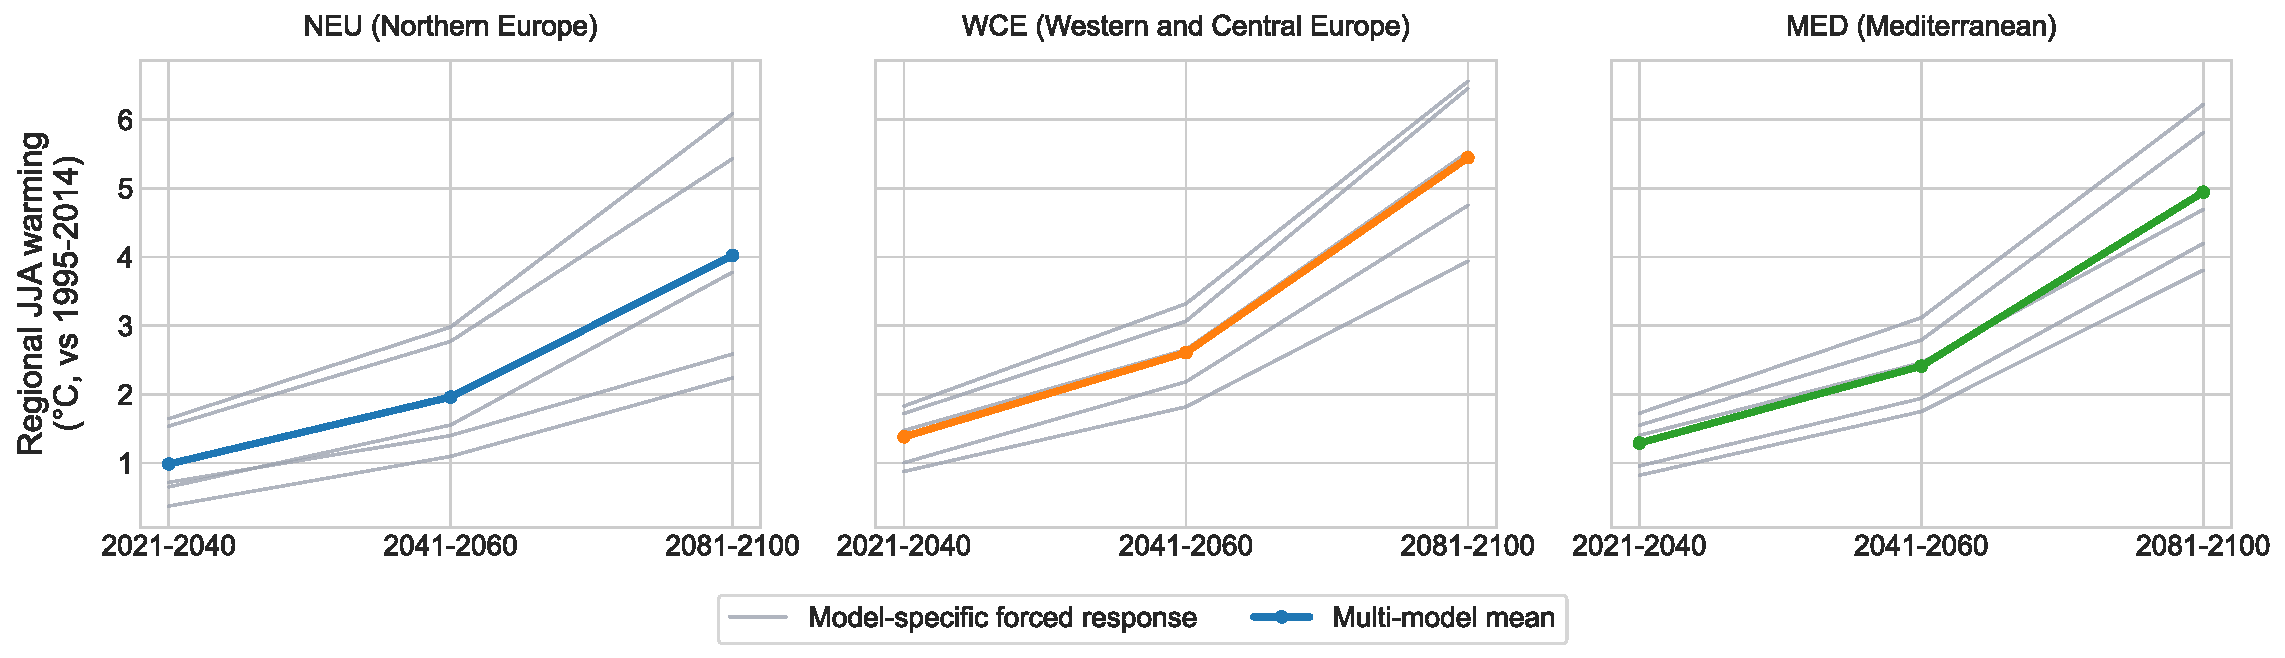
\includegraphics[width=1\linewidth]{work/01-climate_uncertainty/figures/fig02_regional_jja_warming_timeseries} 

}

\caption{Regional JJA warming across the three future periods. Gray lines show model-specific forced responses, while the highlighted line shows the equal-model-weighted multi-model mean.}\label{fig:unc-regional-jja-warming}
\end{figure}

The regional ranking is consistent across the three periods: WCE shows the largest multi-model mean warming, followed by MED and NEU. By 2081--2100, mean warming ranges from about \(4.0^\circ\mathrm{C}\) in NEU to about \(5.4^\circ\mathrm{C}\) in WCE, showing substantial but spatially uneven regional summer warming.

The multi-model mean does not show how strongly the individual model responses differ. Figure \ref{fig:unc-model-forced-response} therefore compares the model-specific forced responses directly. All five models project increasing warming, but their responses separate more clearly with projection lead time.

\begin{figure}

{\centering 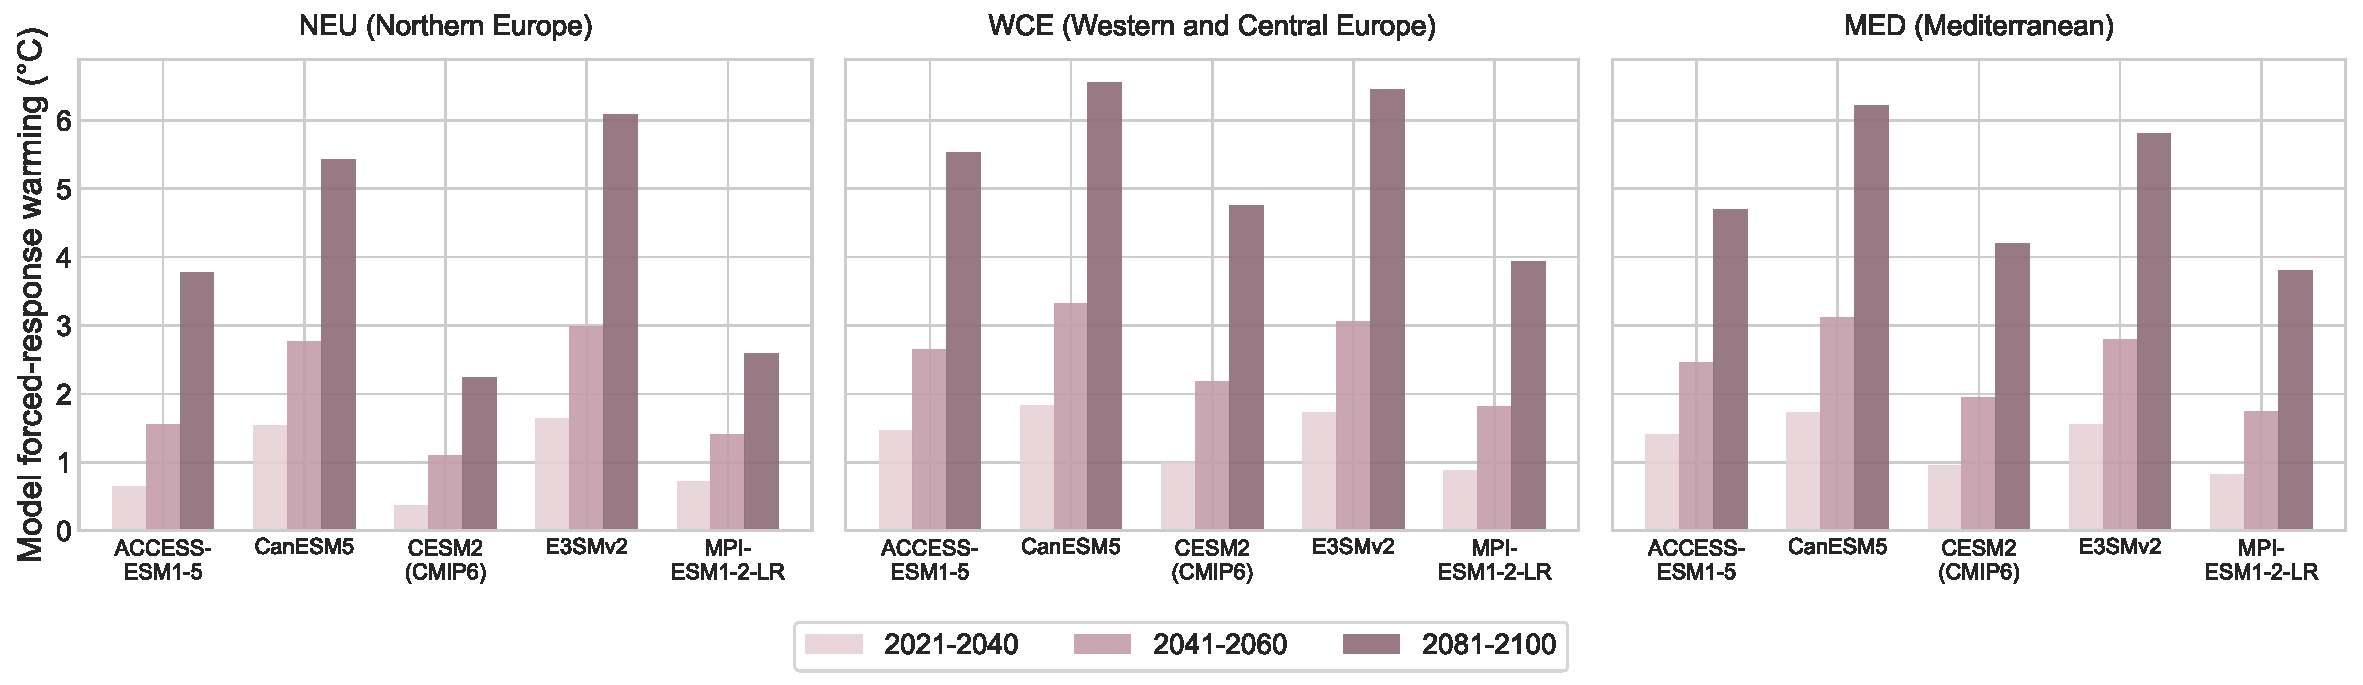
\includegraphics[width=1\linewidth]{work/01-climate_uncertainty/figures/fig03_model_forced_response} 

}

\caption{Model-specific forced regional JJA warming responses across the three study regions and future periods.}\label{fig:unc-model-forced-response}
\end{figure}

The divergence is strongest toward the late century and is particularly pronounced in NEU, where the model-specific responses span roughly \(2.2\)--\(6.1^\circ\mathrm{C}\). Thus, the selected models consistently project substantial regional summer warming under SSP3-7.0, while differing considerably in its magnitude. This increasing separation among model-specific forced responses provides the empirical basis for the model-uncertainty results examined in the following section.

\subsection{Changing Structure of Projection Uncertainty}\label{changing-structure-of-projection-uncertainty}

The uncertainty components show different temporal patterns. Internal variability remains relatively stable across the three future periods, while model uncertainty increases substantially with projection lead time. As a result, total fixed-scenario uncertainty also increases over time and becomes increasingly dominated by differences among model responses.

Internal standard deviation varies more across regions than across future periods. MED consistently shows the lowest internal variability, while NEU and WCE show somewhat larger within-model spread (Figure \ref{fig:unc-internal-variability}). Despite these regional differences, there is little evidence of a strong temporal increase in internal variability.

\begin{figure}

{\centering 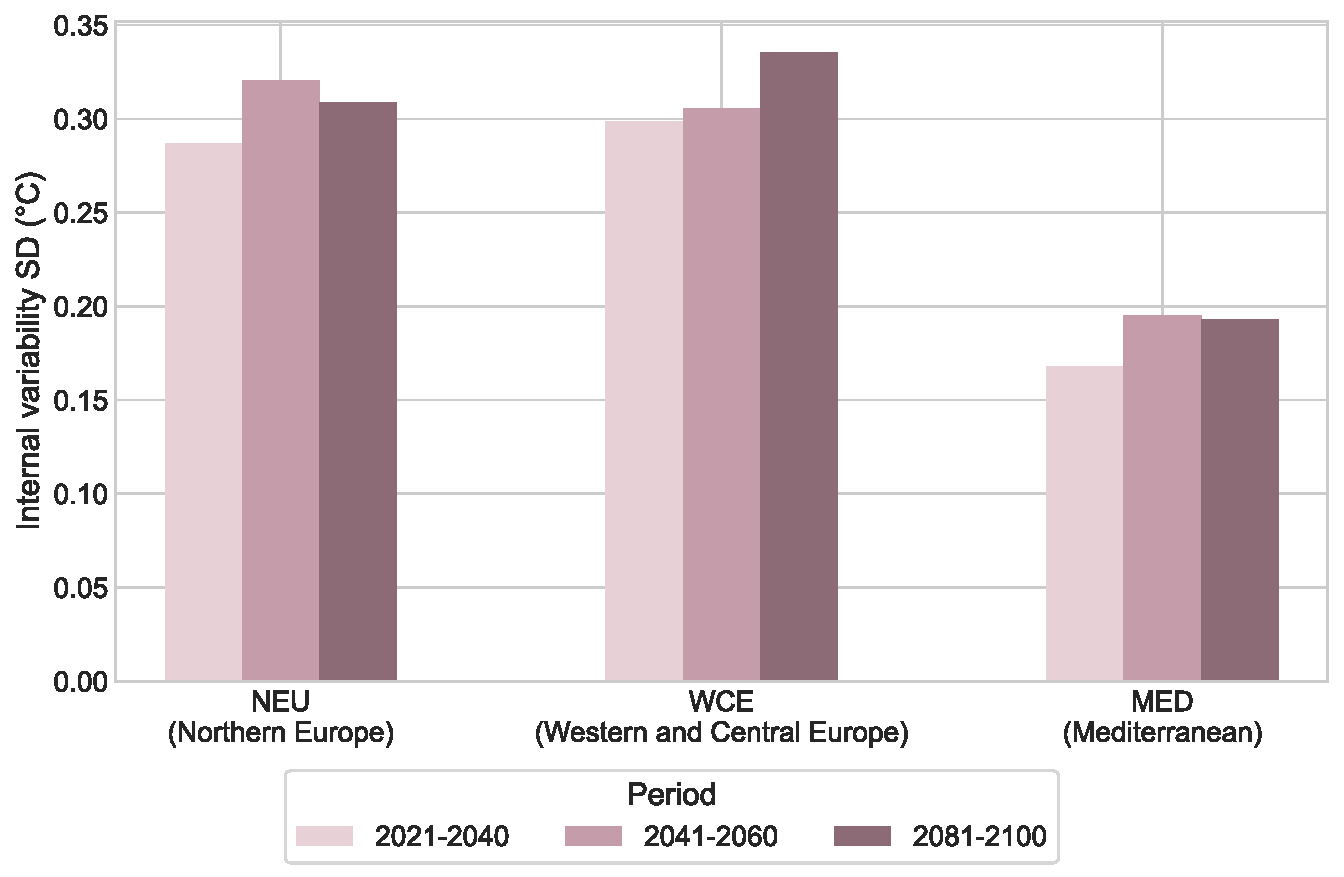
\includegraphics[width=0.65\linewidth]{work/01-climate_uncertainty/figures/fig04_internal_variability} 

}

\caption{Internal variability in 20-year mean regional JJA warming across regions and future periods.}\label{fig:unc-internal-variability}
\end{figure}

Model uncertainty shows a much clearer temporal increase (Figure \ref{fig:unc-model-uncertainty}). The spread among model-specific forced responses becomes wider from the near term to the late century in all regions, with the strongest increase in NEU. Regional contrasts in model uncertainty therefore become more pronounced toward the end of the century.

\begin{figure}

{\centering 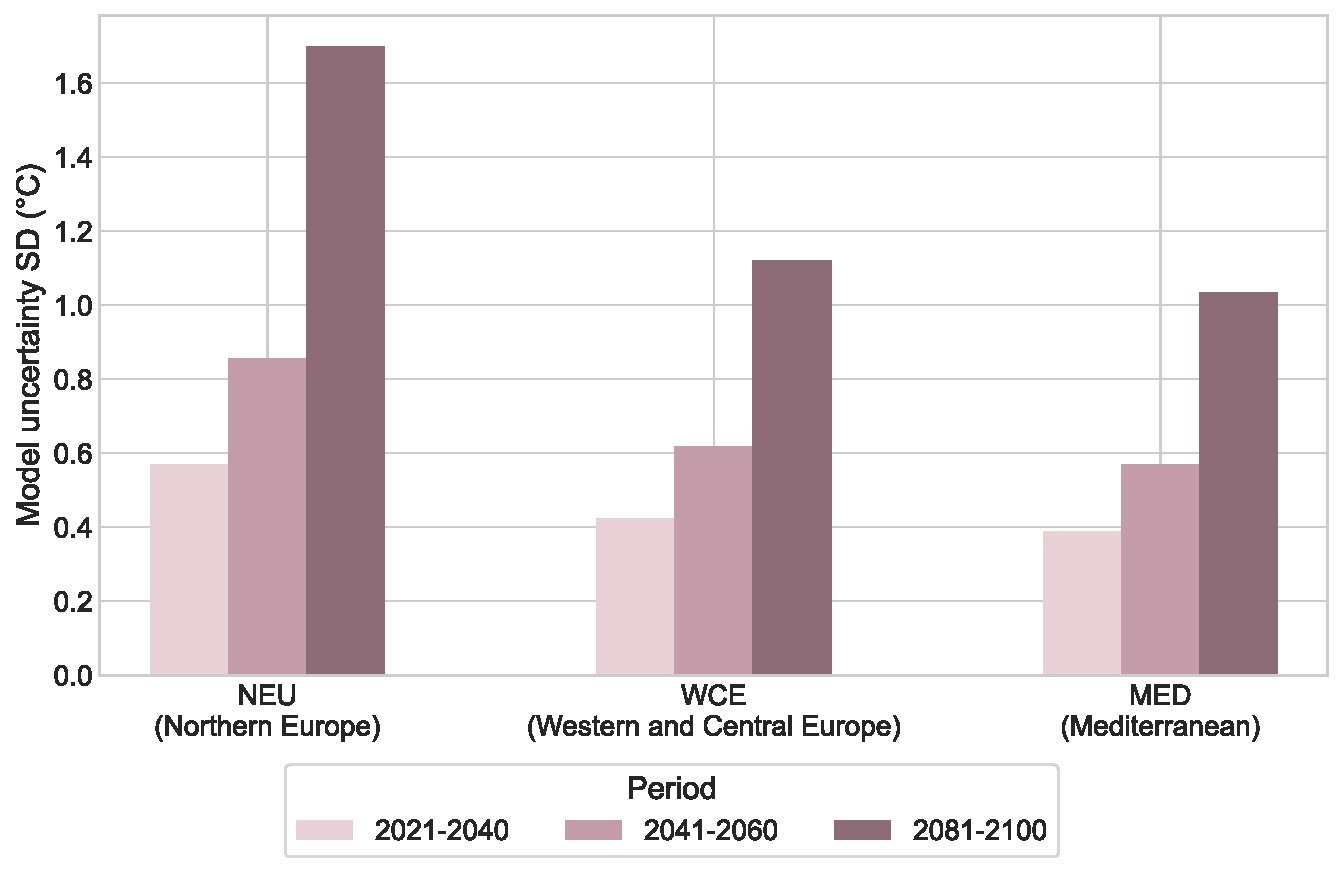
\includegraphics[width=0.65\linewidth]{work/01-climate_uncertainty/figures/fig05_model_uncertainty} 

}

\caption{Model uncertainty in regional JJA warming across regions and future periods.}\label{fig:unc-model-uncertainty}
\end{figure}

The contribution rates confirm that model uncertainty is the larger variance component throughout the analysis (Figure \ref{fig:unc-uncertainty-decomposition}). Its contribution increases with projection lead time, while the relative contribution of internal variability declines. By the late century, model uncertainty accounts for more than 90\% of total variance in all three regions. This change is mainly driven by the growth of model variance rather than by a strong decline in the absolute magnitude of internal variability.

\begin{figure}

{\centering 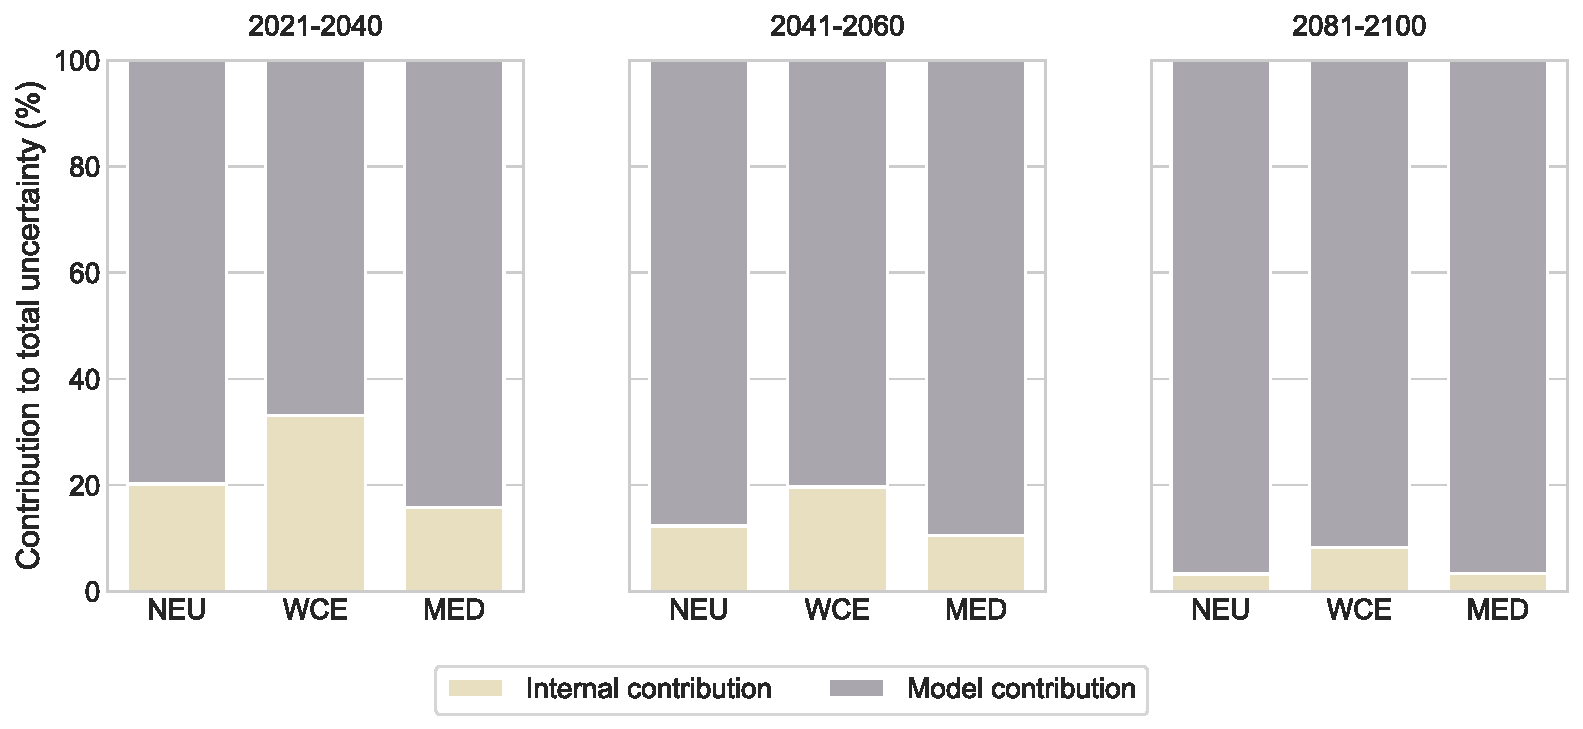
\includegraphics[width=0.8\linewidth]{work/01-climate_uncertainty/figures/fig06_uncertainty_decomposition} 

}

\caption{Relative contributions of internal variability and model uncertainty to total fixed-scenario projection variance.}\label{fig:unc-uncertainty-decomposition}
\end{figure}

Total uncertainty increases across the century in all regions and follows the temporal pattern of model uncertainty closely (Figure \ref{fig:unc-total-uncertainty}). NEU has the highest total uncertainty across the three periods and also shows the strongest late-century spread. Overall, the results indicate that internal variability remains comparatively stable, whereas growing differences among model responses increasingly determine the width of the fixed-scenario projection uncertainty.

\begin{figure}

{\centering 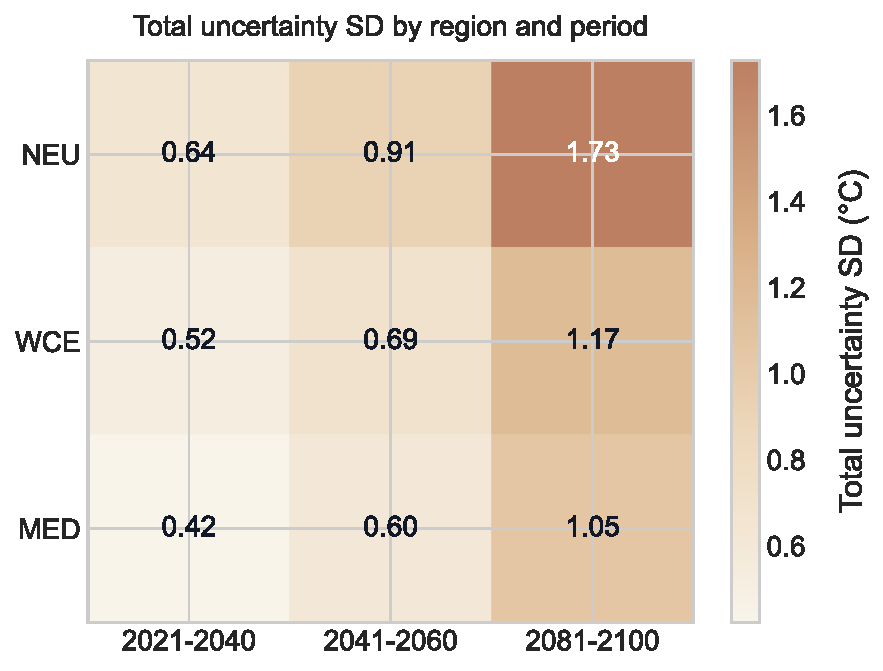
\includegraphics[width=0.5\linewidth]{work/01-climate_uncertainty/figures/fig07_total_uncertainty_heatmap} 

}

\caption{Total fixed-scenario projection uncertainty, expressed as standard deviation, across regions and future periods.}\label{fig:unc-total-uncertainty}
\end{figure}

\subsection{Consequences of Uncertainty for Projection Interpretation}\label{consequences-of-uncertainty-for-projection-interpretation}

To examine what the changing uncertainty structure means for regional climate projections, the analysis next considers the warming distributions beyond their variance components alone. The results are evaluated through prediction ranges, signal-to-noise ratios, and threshold exceedance probabilities, which describe projection spread, signal clarity, and the position of projected warming relative to selected thresholds.

\subsubsection{Widening Projection Ranges and Regional Contrasts}\label{widening-projection-ranges-and-regional-contrasts}

The equal-model-weighted warming distributions widen from the near term to the late century in all three regions (Figure \ref{fig:unc-prediction-ranges}). The increase is most pronounced in NEU, while MED consistently shows the narrowest distribution and WCE remains intermediate.

\begin{figure}

{\centering 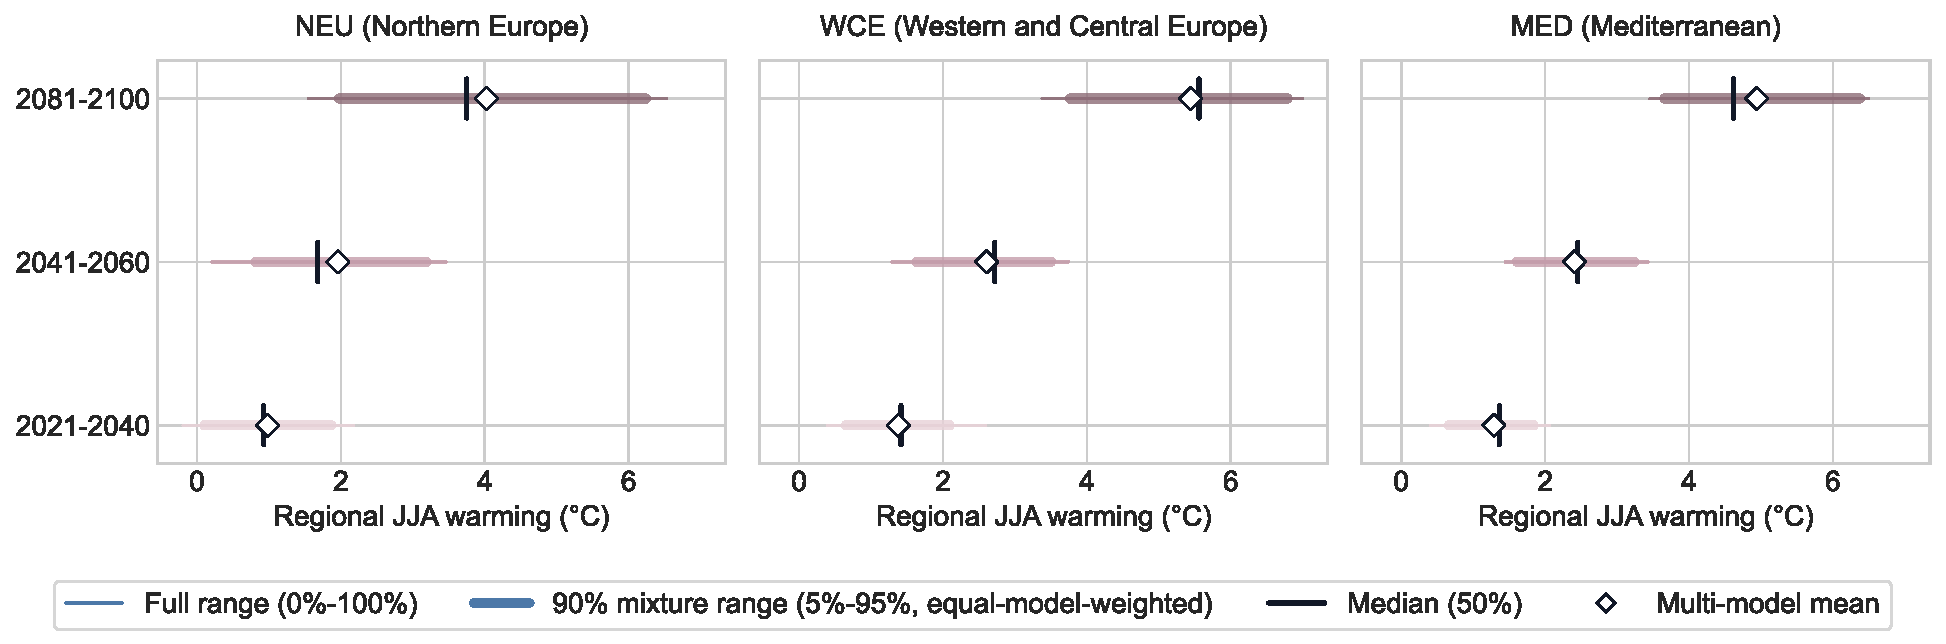
\includegraphics[width=1\linewidth]{work/01-climate_uncertainty/figures/fig08_warming_distribution_prediction_ranges} 

}

\caption{Equal-model-weighted distributions of 20-year mean regional JJA warming and central 90\% prediction ranges across regions and future periods.}\label{fig:unc-prediction-ranges}
\end{figure}

Regional contrasts become clearest in the late-century period. NEU has the widest central 90\% prediction range, reaching a width of about \(4.3^\circ\mathrm{C}\), even though its multi-model mean warming is lower than in MED and WCE. WCE, by contrast, shows the highest mean warming but not the widest projection range. This demonstrates that the magnitude of projected warming and the spread of projected outcomes do not necessarily change together.

The weighted medians remain broadly close to the corresponding multi-model mean warming values across regions and periods. This indicates that the centers of the empirical distributions are generally similar under the two summaries, without implying that the distributions are normally distributed. Overall, the results show a clear widening of projection ranges over time together with persistent regional differences in both central warming and distributional spread.

\subsubsection{Signal Emergence and Total Signal Clarity}\label{signal-emergence-and-total-signal-clarity}

The signal-to-noise ratios show that the projected warming signal is larger than the selected uncertainty scale in all regions and future periods. Total SNR is greater than one for every region-period combination, indicating that mean regional warming exceeds total fixed-scenario uncertainty as measured by the total standard deviation (Figure \ref{fig:unc-total-snr}).

\begin{figure}

{\centering 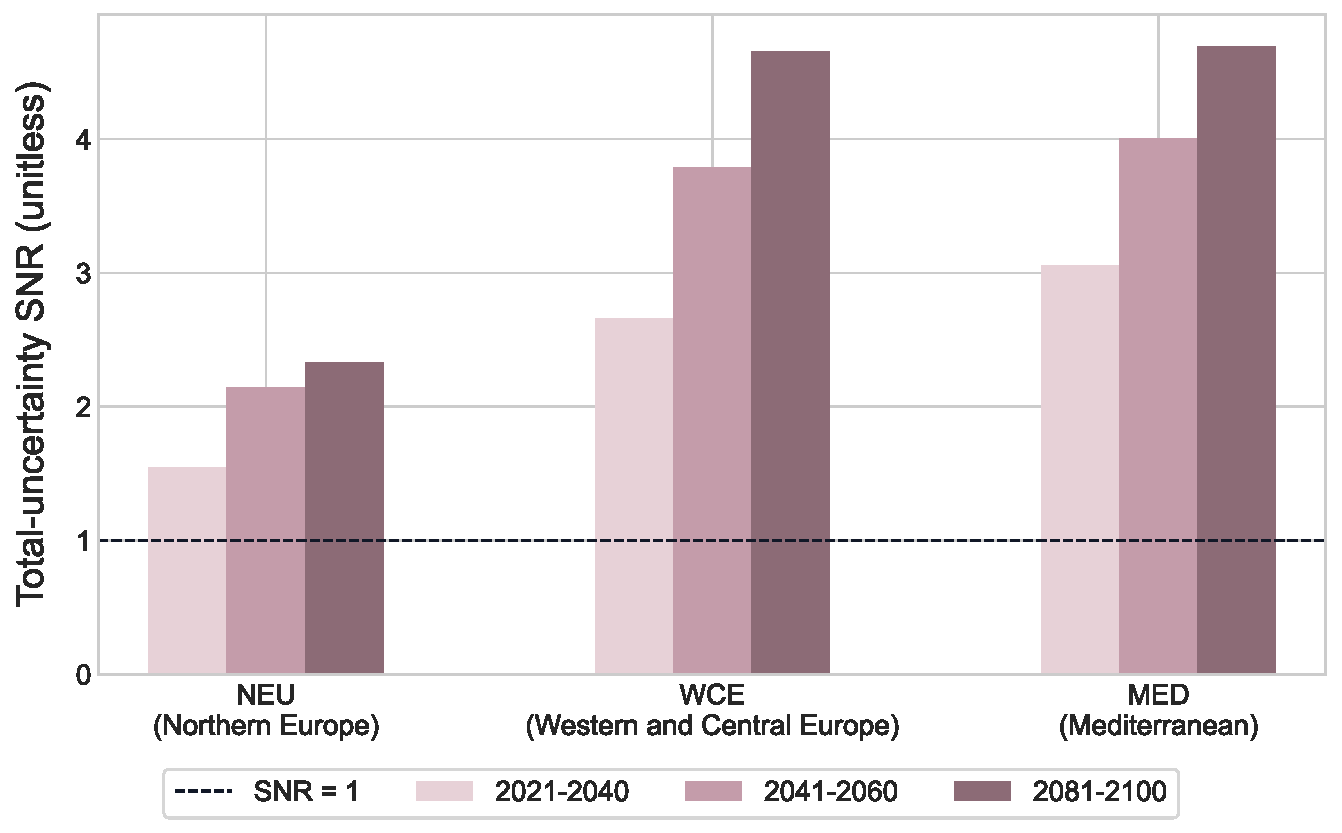
\includegraphics[width=0.65\linewidth]{work/01-climate_uncertainty/figures/fig09_total_snr} 

}

\caption{Total signal-to-noise ratios for regional JJA warming across regions and future periods.}\label{fig:unc-total-snr}
\end{figure}

Clear regional differences remain after both internal and model uncertainty are included. NEU has the lowest total SNR across the three periods, whereas MED and WCE show substantially clearer signals by the late century. Thus, warming is evident relative to total fixed-scenario uncertainty in all three regions, but the clarity of its projected magnitude differs regionally.

Internal SNR is much higher than total SNR in all regions, particularly in the later periods (Figure \ref{fig:unc-internal-snr}). This indicates that the warming signal is large relative to member-to-member variability in 20-year mean warming.

\begin{figure}

{\centering 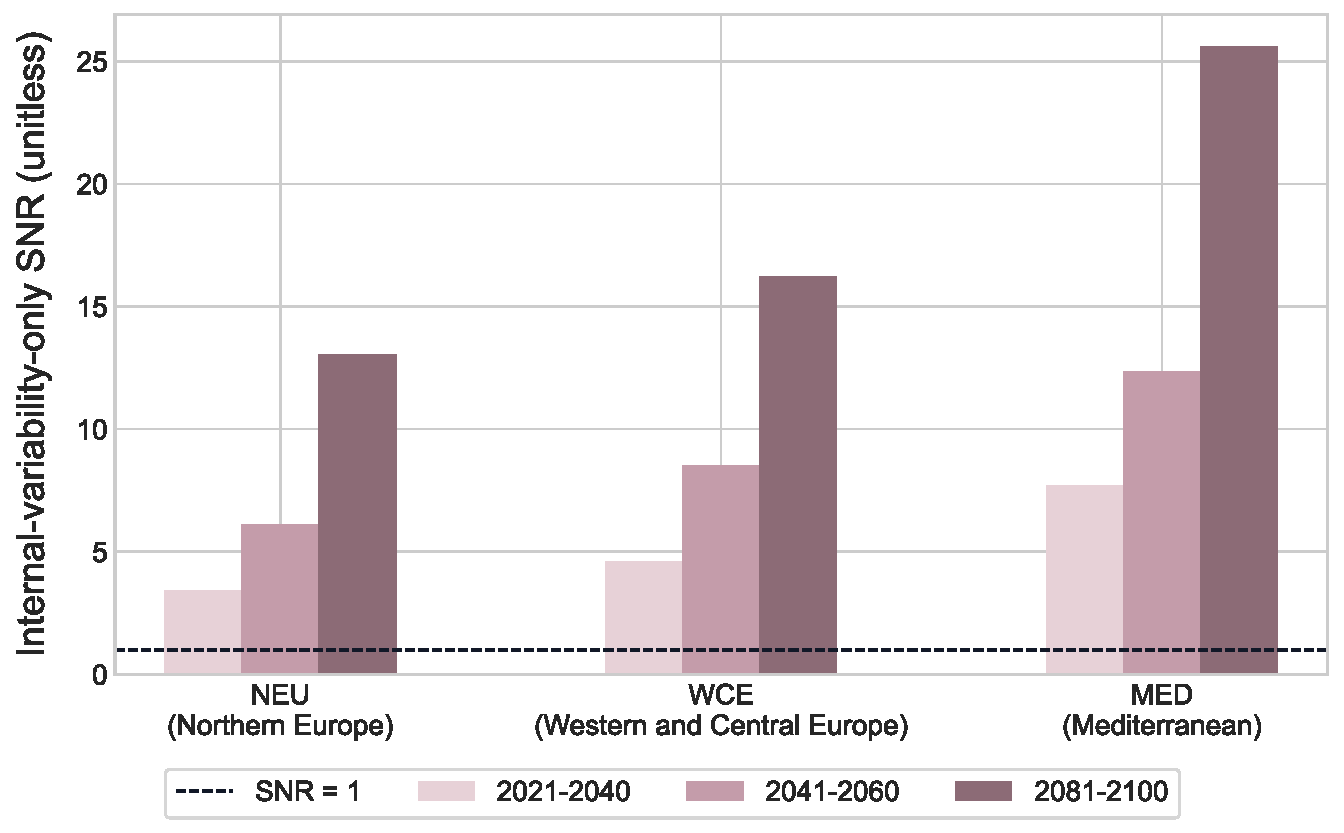
\includegraphics[width=0.65\linewidth]{work/01-climate_uncertainty/figures/fig10_internal_snr} 

}

\caption{Internal signal-to-noise ratios for regional JJA warming across regions and future periods.}\label{fig:unc-internal-snr}
\end{figure}

The contrast between the two SNR measures is consistent across the regional projections. Internal variability alone produces relatively little ambiguity about the direction of warming, while the inclusion of differences among model responses substantially lowers total signal clarity. The warming signal therefore emerges clearly from internal variability, even though uncertainty in its exact magnitude remains larger when model disagreement is included.

\subsubsection{Distributional Spread and Threshold Risk}\label{distributional-spread-and-threshold-risk}

Threshold exceedance probabilities increase strongly as the regional warming distributions shift toward higher temperatures (Figure \ref{fig:unc-threshold-exceedance}). In the near-term period, exceedance of \(2^\circ\mathrm{C}\) is uncommon in all three regions, while no ensemble members exceed \(3^\circ\mathrm{C}\). By mid-century, the regional contrast becomes clearer: exceedance of \(2^\circ\mathrm{C}\) is more likely than not in WCE and MED, but remains below one half in NEU. Exceedance of \(3^\circ\mathrm{C}\) is still substantially less likely in all three regions.

\begin{figure}

{\centering 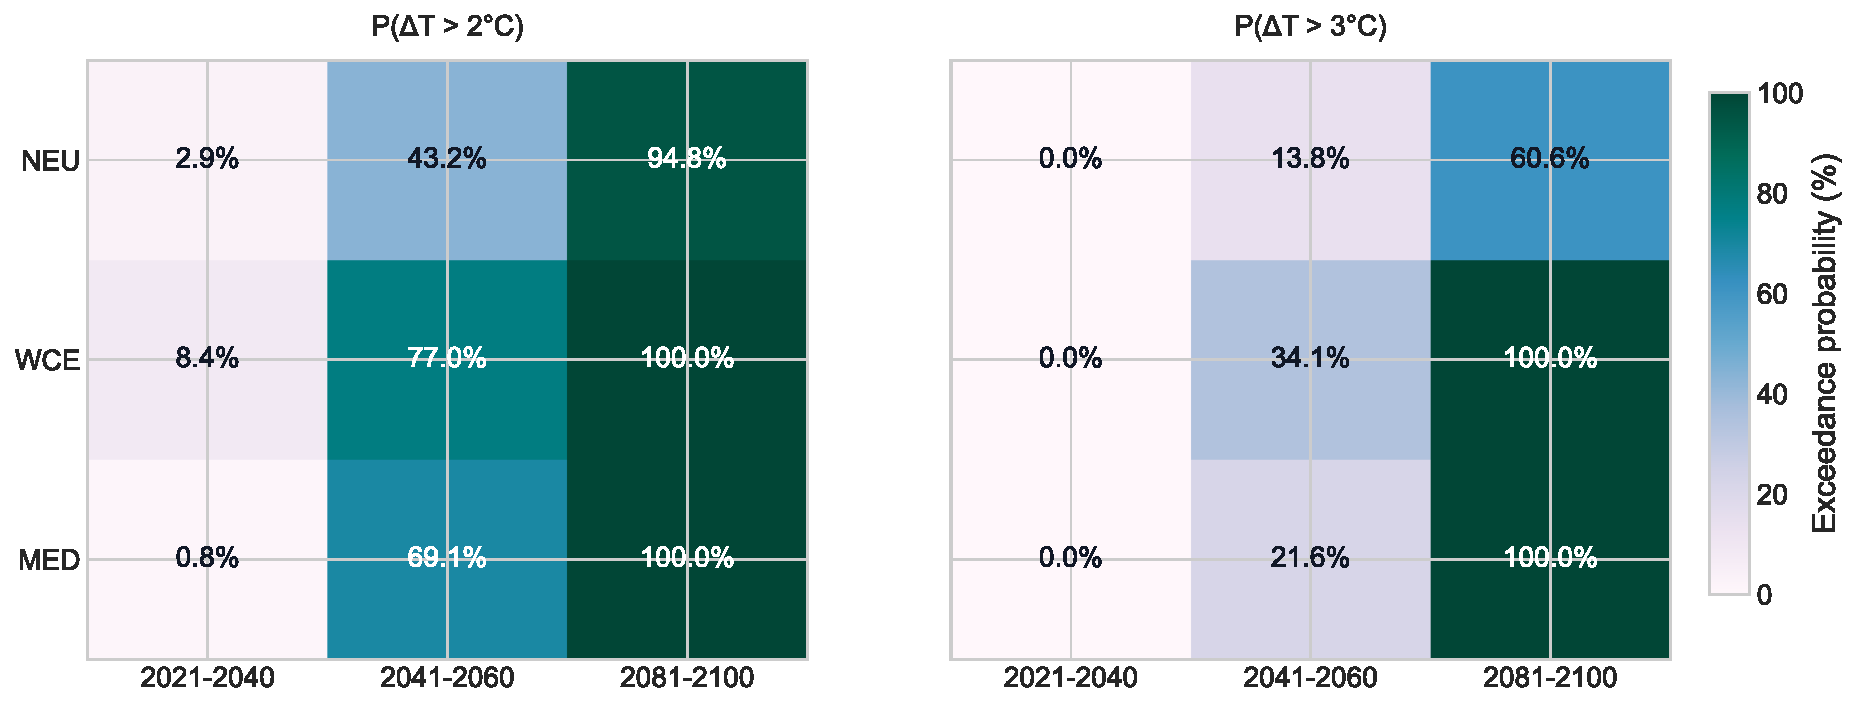
\includegraphics[width=1\linewidth]{work/01-climate_uncertainty/figures/fig11_threshold_exceedance_probability} 

}

\caption{Equal-model-weighted probabilities that regional 20-year mean JJA warming exceeds 2°C and 3°C relative to the 1995--2014 baseline.}\label{fig:unc-threshold-exceedance}
\end{figure}

The mid-century distributions help explain these regional differences (Figure \ref{fig:unc-mid-century-threshold-distributions}). In NEU, much of the model-member distribution remains below the \(2^\circ\mathrm{C}\) threshold, whereas larger shares of the WCE and MED distributions lie above it. The \(3^\circ\mathrm{C}\) threshold remains in the upper part of all three distributions. Mid-century therefore provides a clear example of how the position of a threshold relative to both the center and spread of a distribution affects exceedance probability.

\begin{figure}

{\centering 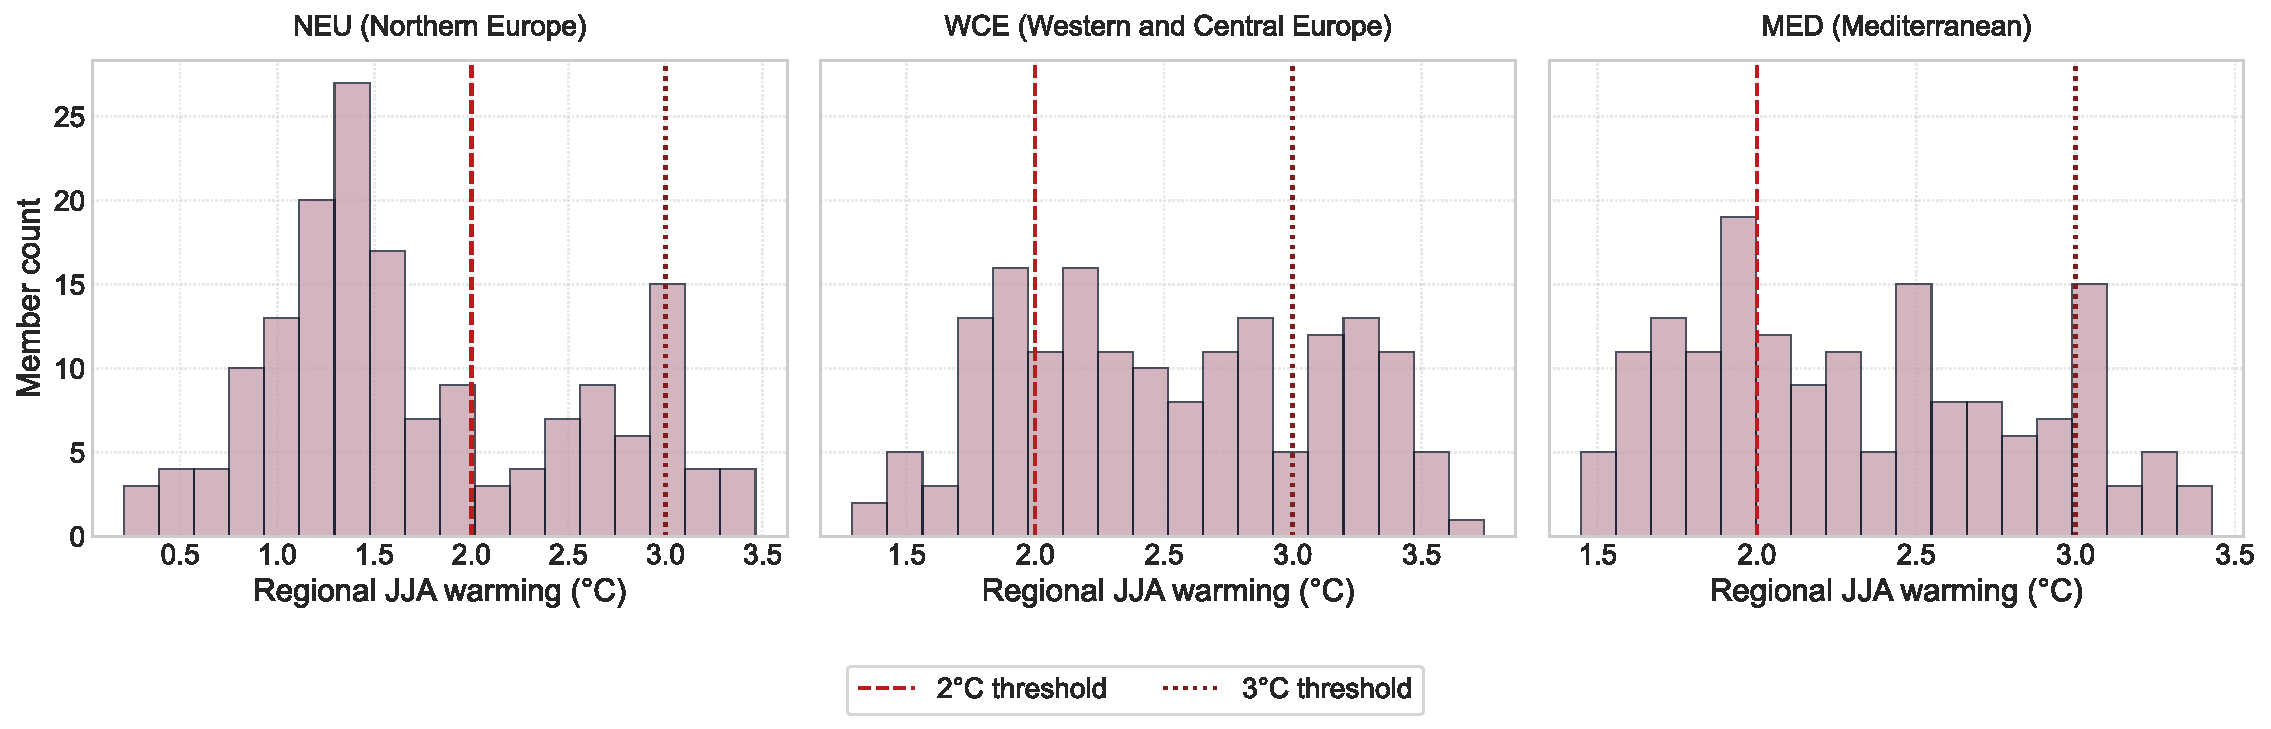
\includegraphics[width=1\linewidth]{work/01-climate_uncertainty/figures/fig15b_mid_century_warming_distribution_thresholds} 

}

\caption{Mid-century model-member distributions of regional 20-year mean JJA warming relative to the 2°C and 3°C thresholds.}\label{fig:unc-mid-century-threshold-distributions}
\end{figure}

By 2081--2100, both thresholds are exceeded by all ensemble members in MED and WCE. NEU also shows a high probability of exceeding \(2^\circ\mathrm{C}\), but its \(3^\circ\mathrm{C}\) exceedance probability remains lower, at approximately 60.6\%. Its wider warming distribution therefore leaves a substantial share of projected outcomes below the higher threshold even in the late-century period.

Together, the probability estimates and mid-century distributions show that threshold exceedance cannot be inferred from mean warming alone. The resulting probability depends on where the threshold lies within the projected distribution as well as on the distributional spread. These probabilities refer to 20-year mean regional JJA warming relative to 1995--2014 and should therefore be interpreted as conditional, ensemble-based risk-style diagnostics rather than probabilities for individual summers.

\subsection{Robustness of the Main Findings}\label{robustness-of-the-main-findings}

The robustness analyses support the main qualitative patterns identified in the full-member analysis. The hierarchical bootstrap shows that internal-variability estimates are comparatively stable, whereas intervals for model-related quantities, total uncertainty, and contribution rates are wider (Figure \ref{fig:unc-bootstrap-uncertainty}). This greater spread is most visible for quantities that depend strongly on differences among the five model responses.

\begin{figure}

{\centering 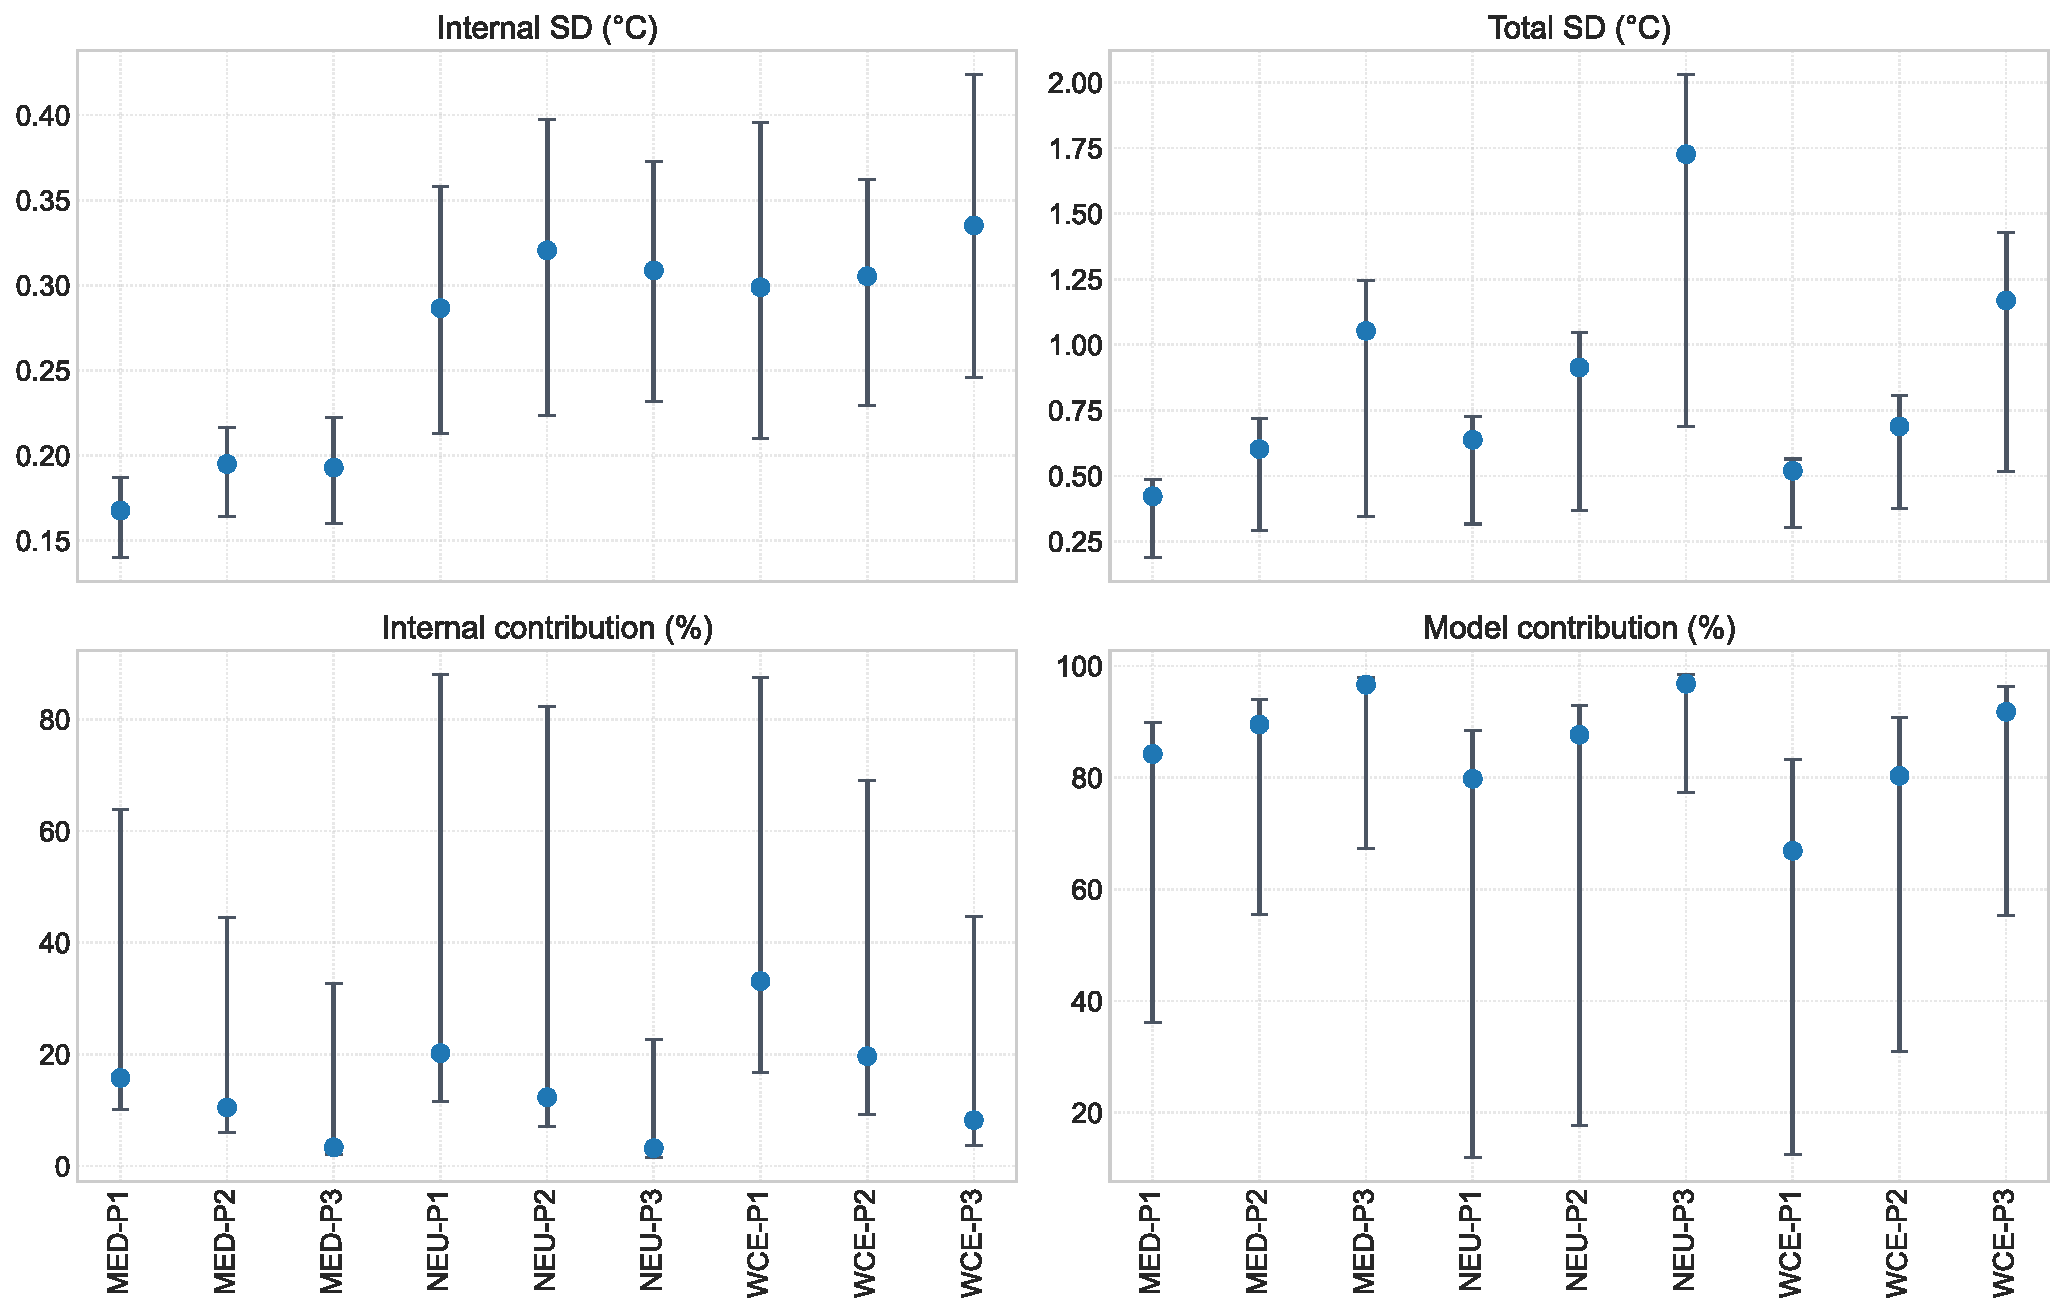
\includegraphics[width=1\linewidth]{work/01-climate_uncertainty/figures/fig16_bootstrap_ci_uncertainty_metrics} 

}

\caption{Hierarchical-bootstrap point estimates and 95\% percentile intervals for selected uncertainty metrics across regions and future periods.}\label{fig:unc-bootstrap-uncertainty}
\end{figure}

The bootstrap results for the distributional diagnostics lead to the same overall interpretation (Figure \ref{fig:unc-bootstrap-diagnostics}). Signal-to-noise results continue to indicate clear warming relative to the analyzed uncertainty scales. Threshold probabilities are less stable when the threshold lies within the central part of the warming distribution, particularly during the mid-century transition, while probabilities already close to zero or one are more stable. These intervals do not change the main temporal and regional patterns reported above.

\begin{figure}

{\centering 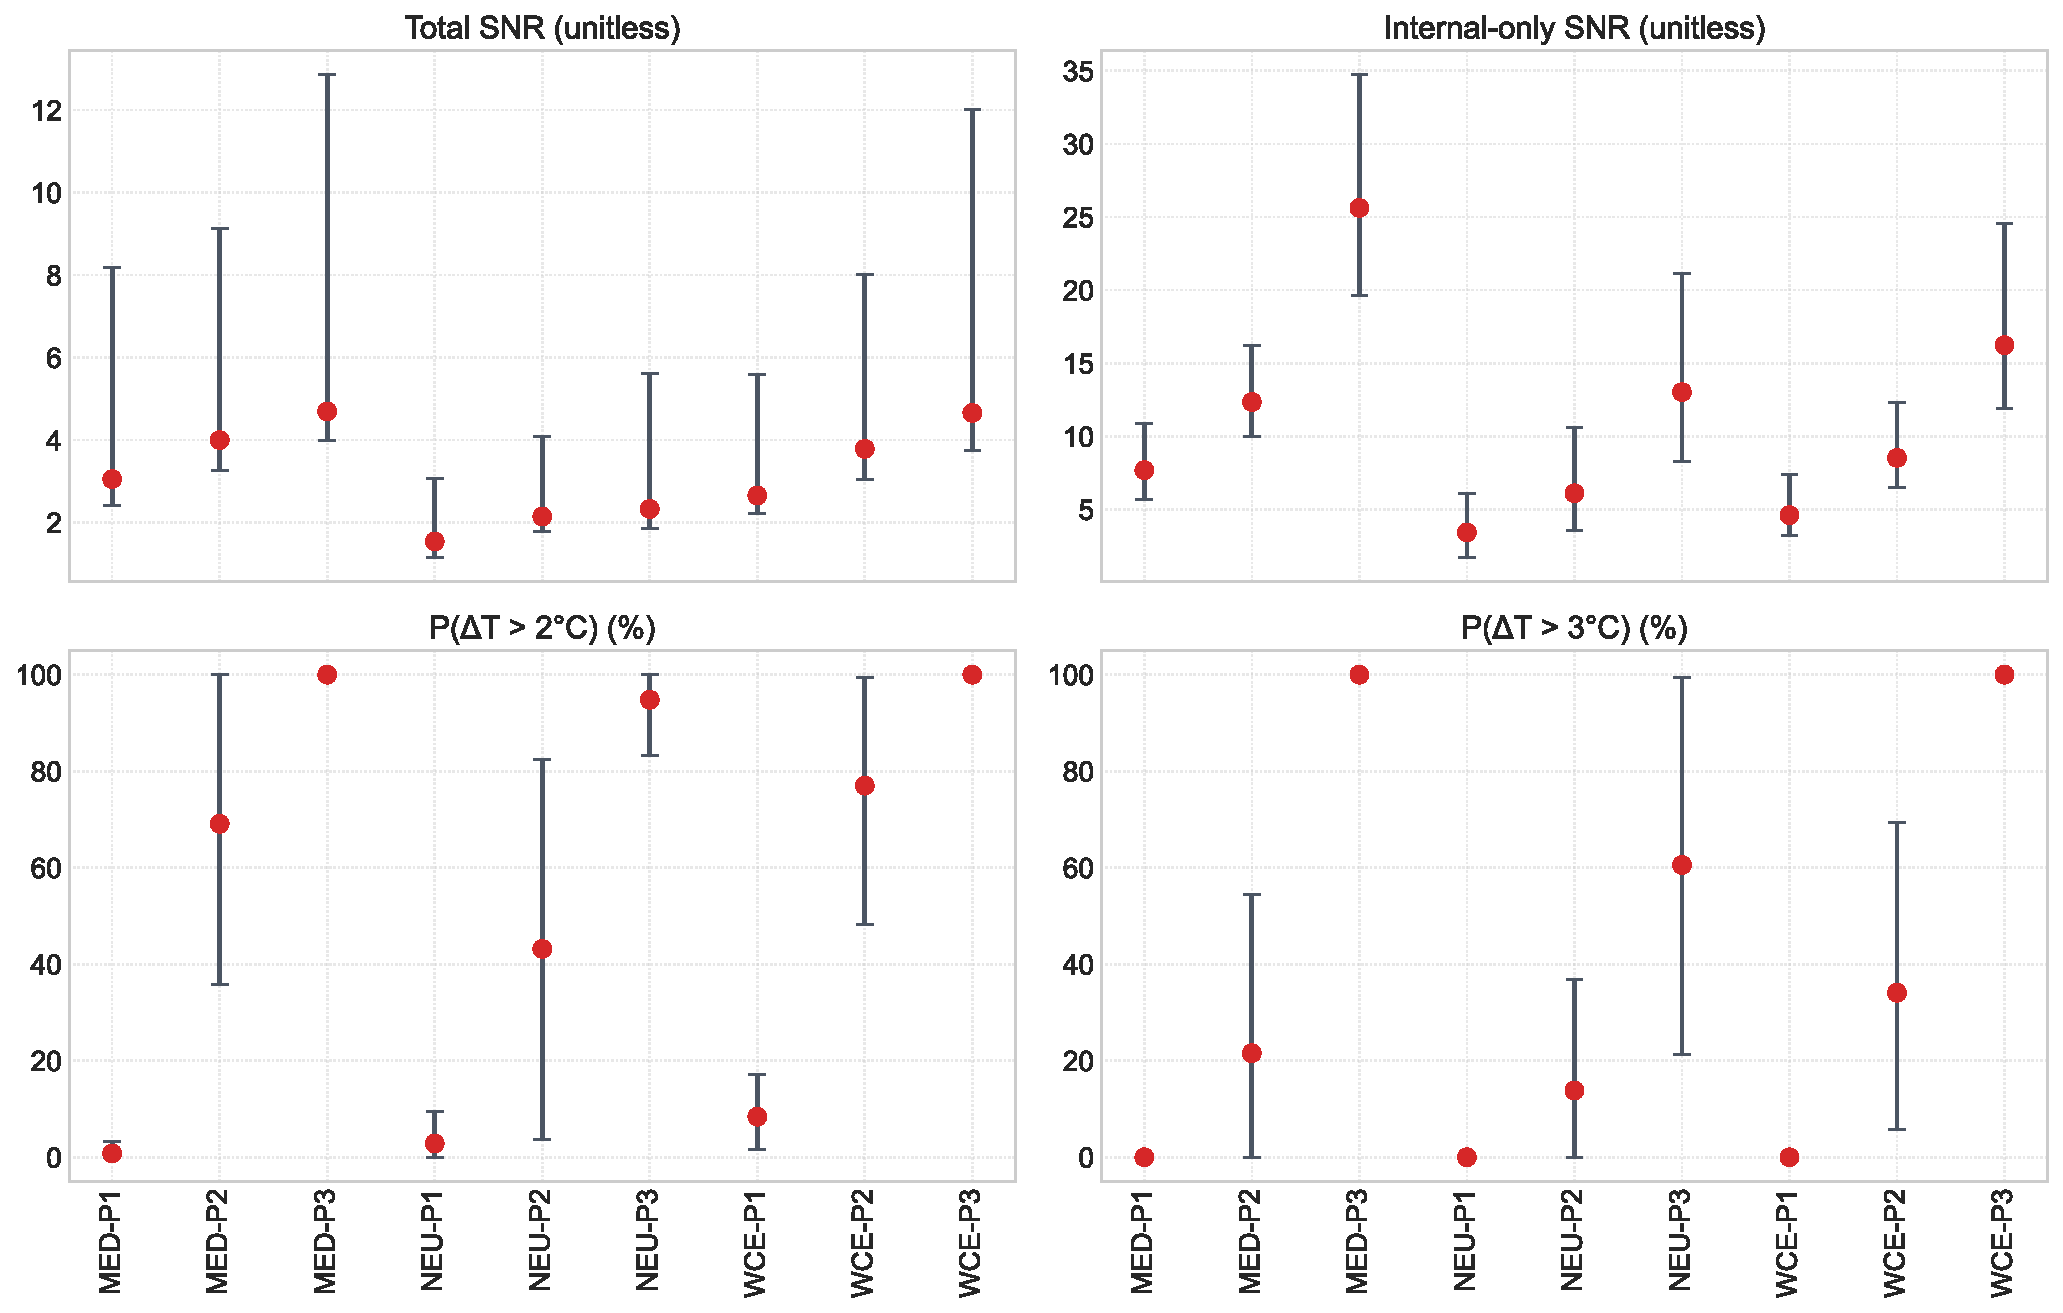
\includegraphics[width=1\linewidth]{work/01-climate_uncertainty/figures/fig17_bootstrap_ci_snr_threshold_probability} 

}

\caption{Hierarchical-bootstrap point estimates and 95\% percentile intervals for signal-to-noise ratios and threshold exceedance probabilities.}\label{fig:unc-bootstrap-diagnostics}
\end{figure}

The balanced-member sensitivity analysis provides a complementary check on the unequal original ensemble sizes. Estimates obtained from repeated 20-member-per-model subsamples remain close to the corresponding full-member estimates, with most comparisons lying near the 1:1 line (Figure \ref{fig:unc-balanced-member-sensitivity}). The regional rankings, temporal increase in model and total uncertainty, and the dominance of model uncertainty are retained. Differences in total standard deviation and total signal-to-noise ratio are also small relative to the main regional and temporal contrasts.

\begin{figure}

{\centering 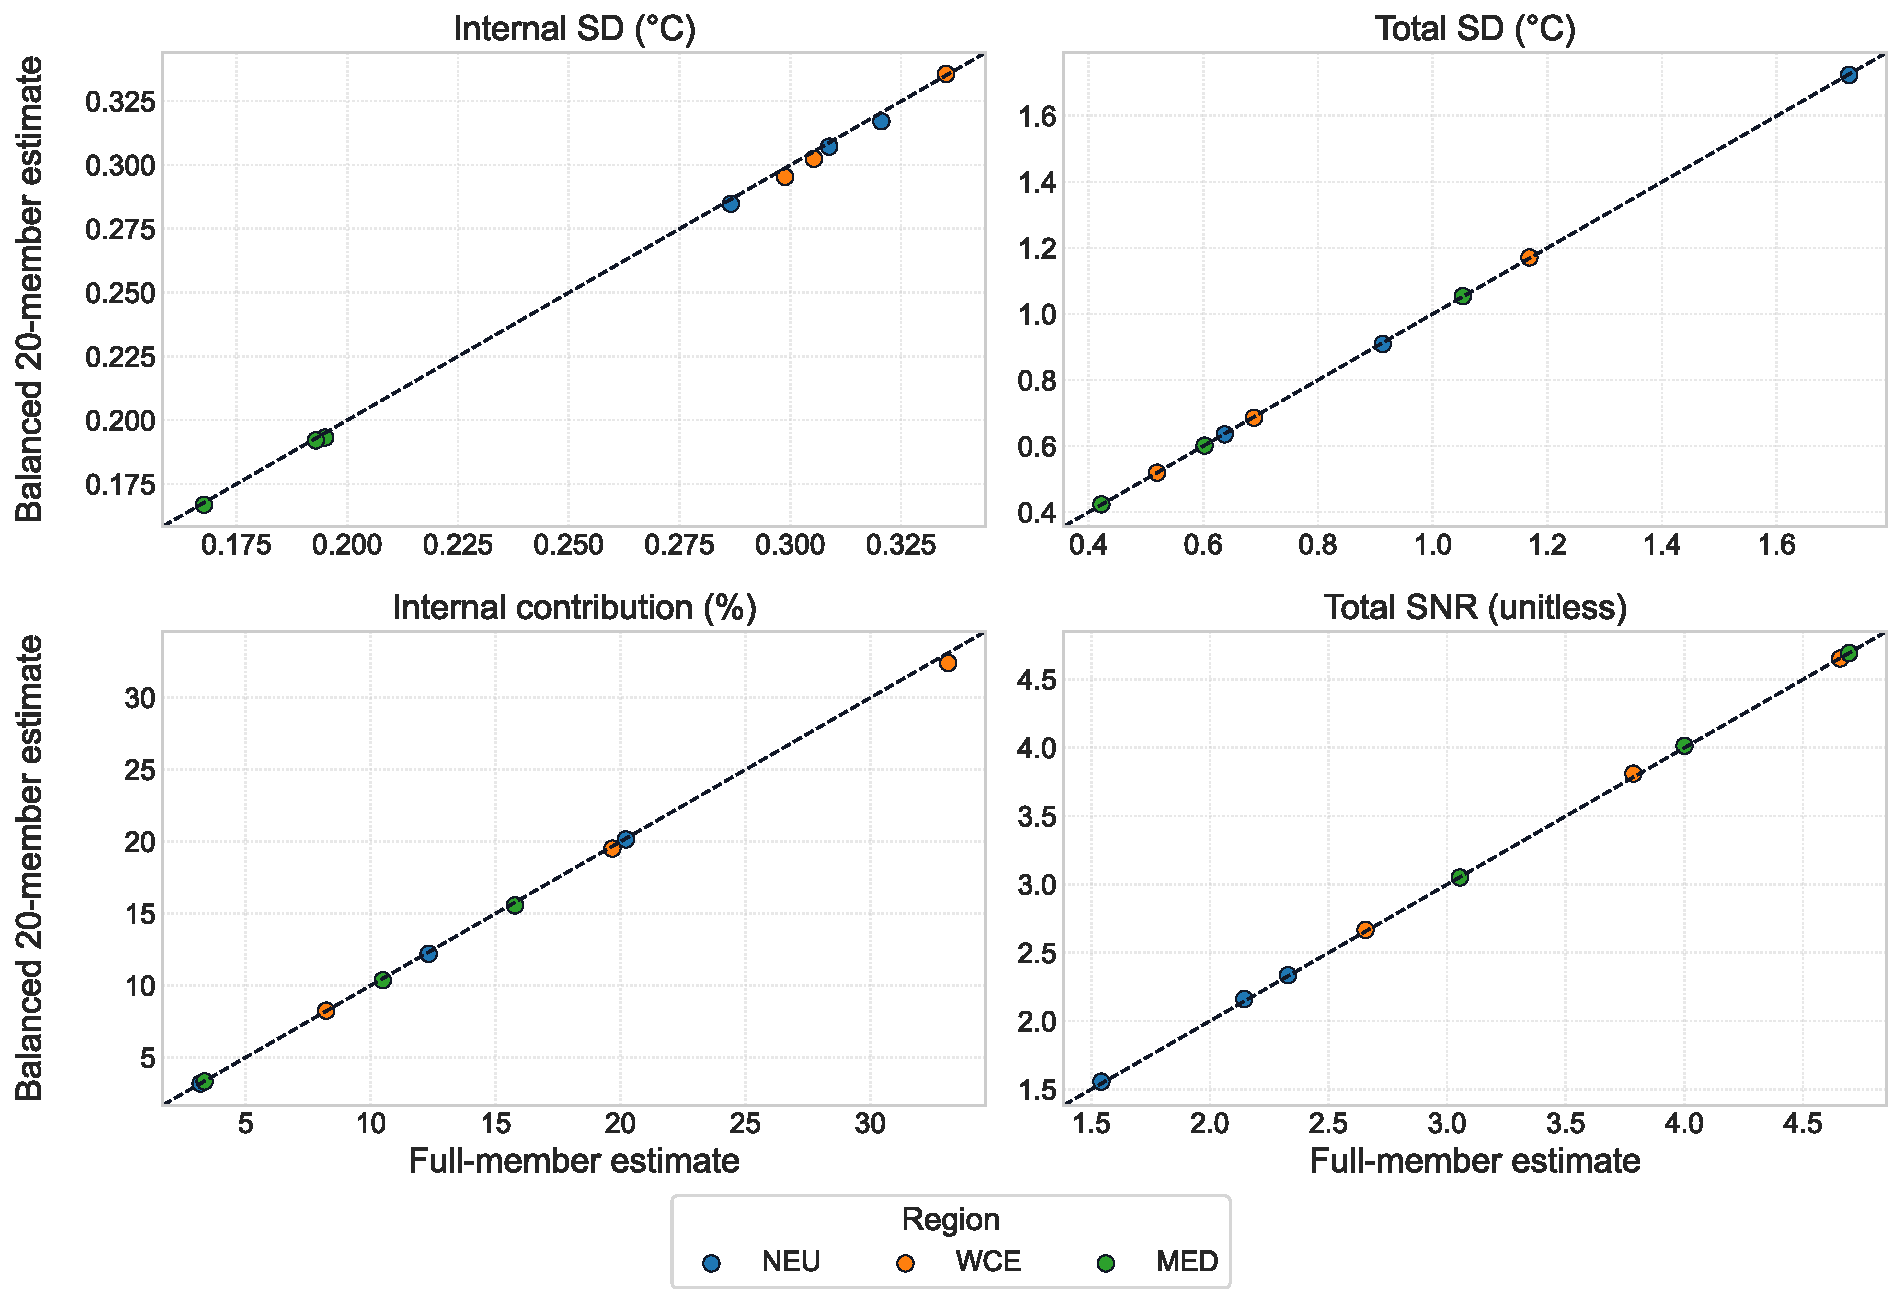
\includegraphics[width=1\linewidth]{work/01-climate_uncertainty/figures/fig18_balanced_20_member_sensitivity} 

}

\caption{Comparison of full-member estimates with estimates from the balanced 20-member-per-model sensitivity analysis. The diagonal represents exact agreement.}\label{fig:unc-balanced-member-sensitivity}
\end{figure}

Overall, both robustness checks support the central conclusions of the analysis. Unequal ensemble sizes do not appear to drive the main findings, while the bootstrap confirms that estimates based on between-model differences are less tightly constrained than estimates of within-model variability. The exact magnitude of model uncertainty and its contribution nevertheless remains conditional on the selected five-model ensemble.

\section{Discussion}\label{discussion}

The results show that the interpretation of projection uncertainty depends not only on its magnitude, but also on how the projection target is defined. The discussion therefore focuses on the role of 20-year temporal averaging in the uncertainty decomposition, the distinction between signal emergence and model agreement, and how the findings should be interpreted in relation to previous work and the conditional scope of the analysis.

\subsection{Temporal Averaging and the Dominance of Model Uncertainty}\label{temporal-averaging-and-the-dominance-of-model-uncertainty}

The strong contribution of model uncertainty should be interpreted in relation to the temporal scale of the prediction target. The uncertainty decomposition is applied to 20-year mean regional JJA warming, as defined in Equation \eqref{eq:unc-period-mean-warming}, rather than to annual temperature anomalies. Internal variability therefore describes differences among ensemble members in their 20-year mean warming. Averaging over a longer period allows positive and negative short-term deviations to partly cancel, reducing the member-to-member spread of the period means \citep{Hawkins2009}.

A simple statistical approximation illustrates this effect. For a temporally varying quantity \(X\),

\[
\operatorname{Var}(\overline{X})
\approx
\frac{\sigma^2}{n_{\mathrm{eff}}},
\]

where \(\sigma^2\) is the variance at the shorter time scale and \(n_{\mathrm{eff}}\) is the effective number of independent observations contributing to the mean. Because climate values can be autocorrelated, \(n_{\mathrm{eff}}\) may be smaller than the 20 years contained in each period. Nevertheless, averaging still suppresses part of the short-term variability that would be more visible in annual or shorter-period indicators.

This helps explain the uncertainty pattern found in the analysis. Internal standard deviation changes relatively little across the future periods, while the spread among model-specific forced responses grows substantially. Temporal averaging reduces the influence of member-specific fluctuations on the 20-year target, but persistent differences among model responses are not removed in the same way. As these between-model differences increase with projection lead time, they account for an increasing share of total fixed-scenario variance (Figure \ref{fig:unc-uncertainty-decomposition}).

The resulting decline in the internal contribution should therefore not be interpreted as evidence that internal variability is generally unimportant. It means that internal variability contributes relatively little to the specific quantity analyzed here: 20-year mean regional summer warming. A different prediction target, such as annual temperature, a shorter averaging period, or a smaller spatial scale, could retain more internal variability and produce a different uncertainty balance.

This scale dependence is consistent with Hawkins and Sutton, who explicitly considered the effect of temporal averaging in their uncertainty framework and mainly analyzed decadal mean temperature projections \citep{Hawkins2009}. Their results also show that the relative importance of internal and model uncertainty changes with prediction horizon and averaging scale. The particularly high model contribution found here is therefore plausibly influenced by the use of 20-year means, but temporal averaging should not be treated as the only explanation. The selected models, regional and seasonal aggregation, fixed forcing pathway, weighting scheme, and variance estimators can also affect the estimated contribution rates.

\subsection{Signal Emergence, Model Disagreement, and Risk Interpretation}\label{signal-emergence-model-disagreement-and-risk-interpretation}

The signal-to-noise results distinguish two related but different questions: whether regional warming is large relative to internal variability, and whether models agree closely on the magnitude of that warming. The high internal SNR values indicate that the warming signal is clearly separated from member-to-member variability in 20-year mean warming (Figure \ref{fig:unc-internal-snr}). This interpretation is consistent with the use of internal variability as the noise component in climate signal-to-noise analysis \citep{Hawkins2009, Gruber2026}. It does not imply that internal variability is negligible at shorter temporal scales or for other climate indicators.

The lower total SNR values show that this clear emergence from internal variability does not translate into equally precise agreement among model projections (Figure \ref{fig:unc-total-snr}). Once differences among model-specific forced responses are included, the uncertainty surrounding the magnitude of warming becomes substantially larger. The selected models therefore agree more strongly on the direction of regional warming than on its exact magnitude. In this sense, \textbf{signal emergence does not imply precise projection agreement}.

The distribution-based diagnostics further show why warming magnitude and uncertainty must be considered jointly. NEU provides the clearest example: although its central warming estimate is lower than in WCE and MED, it has the widest late-century prediction range and the lowest total signal clarity. WCE, by contrast, combines stronger central warming with a narrower distribution than NEU. These differences show that a larger mean response does not necessarily imply greater projection uncertainty, and a smaller mean response does not necessarily imply greater confidence (Figure \ref{fig:unc-prediction-ranges}).

The same distinction is important for interpreting threshold exceedance. Exceedance probability depends on where a threshold lies relative to both the center and the spread of the warming distribution. When most of the distribution has moved beyond a threshold, exceedance becomes consistently high; when the threshold cuts through a wider distribution, substantial uncertainty remains even when the mean warming is above that level (Figure \ref{fig:unc-threshold-exceedance}). This is particularly relevant for NEU at the higher threshold, where the wider distribution produces less certain exceedance than in the other regions.

These threshold probabilities should nevertheless be interpreted narrowly. They are conditional, ensemble-based diagnostics for 20-year mean regional JJA warming relative to the 1995--2014 baseline, rather than complete measures of climate risk. They do not represent the probability of an individual hot summer, nor do the \(2^\circ\mathrm{C}\) and \(3^\circ\mathrm{C}\) thresholds correspond to global warming levels relative to the pre-industrial period. More broadly, the results illustrate the value of interpreting multi-model projections as distributions rather than relying on the ensemble mean alone \citep{Tebaldi2007}.

\subsection{Relation to Previous Work and Overall Interpretation}\label{relation-to-previous-work-and-overall-interpretation}

The main findings are broadly consistent with previous work on uncertainty in climate-model ensembles. Initial-condition large ensembles provide a way to separate member-to-member internal variability from the model-specific forced response, while multiple large ensembles extend this framework to differences among model responses \citep{Deser2020, Lehner2020}. The increasing importance of model uncertainty with projection lead time is also consistent with established climate-projection uncertainty frameworks \citep{Hawkins2009, Lehner2020}. However, the relative contribution of each uncertainty source is not a universal property of climate projections. It depends on the prediction horizon, spatial and temporal scale, climate indicator, model sample, scenario design, and statistical treatment. The contribution rates found here should therefore be interpreted for the specific 20-year regional summer-warming target used in this study rather than compared directly with values obtained for annual or differently aggregated projections.

The analysis also supports the value of combining source-based and distribution-based views of uncertainty. The variance decomposition identifies whether spread arises mainly within models or among model responses, whereas prediction ranges, signal-to-noise ratios, and threshold probabilities describe how that spread affects the interpretation of projected warming. This complements the multi-model distributional perspective emphasized in previous work, where the ensemble mean alone is not sufficient to describe projection uncertainty \citep{Tebaldi2007}. In the present analysis, these different summaries lead to a consistent interpretation: the warming signal is clear, but uncertainty in its exact regional magnitude remains strongly influenced by disagreement among model responses.

The robustness analyses strengthen this qualitative interpretation without removing the dependence on the available model sample. The balanced-member analysis indicates that the dominance of model uncertainty is not simply a consequence of unequal ensemble sizes. At the same time, the hierarchical bootstrap shows that quantities based on between-model differences are less tightly constrained than within-model estimates. This is expected when model uncertainty is estimated from only five model-specific responses. The robustness results therefore support the main regional and temporal patterns, while suggesting more caution in interpreting the exact magnitude of model variance and its contribution rate.

The scope of these conclusions is deliberately conditional. The analysis considers SSP3-7.0 only, five selected large-ensemble models with equal model weight, JJA mean temperature, three European regions, and 20-year warming relative to 1995--2014. Scenario uncertainty is not included, and the \(2^\circ\mathrm{C}\) and \(3^\circ\mathrm{C}\) thresholds refer to regional baseline-relative summer warming rather than global warming levels. Moreover, the spread among the selected models is an empirical representation of model disagreement, not a complete measure of real-world epistemic uncertainty \citep{Gruber2025}.

Overall, the results reinforce a central statistical point: uncertainty attribution depends on both the ensemble being analyzed and the definition of the prediction target. For 20-year mean regional summer warming under a fixed forcing pathway, temporal aggregation limits the relative contribution of within-model variability, while persistent differences among model forced responses become the dominant source of projection spread. Considering uncertainty from several complementary perspectives therefore provides a more informative interpretation than reporting the multi-model mean alone.

\section{Conclusion}\label{conclusion}

This seminar work examined fixed-scenario uncertainty in projected 20-year mean regional JJA warming across NEU, WCE, and MED using five large-ensemble climate models under SSP3-7.0. All regions show increasing summer warming across the century, while the model-specific forced responses become more widely separated with projection lead time. Internal variability in the 20-year warming target remains comparatively stable, whereas model uncertainty increases and becomes the main contributor to total fixed-scenario projection uncertainty.

The distribution-based diagnostics lead to the same overall interpretation from a different perspective. The warming signal is clear relative to internal variability, but agreement on its exact magnitude is reduced when differences among model responses are included. Prediction ranges and threshold exceedance probabilities further show that central warming and projection spread must be considered together: regions with similar or even lower mean warming can still differ substantially in the range and threshold behavior of projected outcomes.

The robustness analyses support these qualitative findings and indicate that unequal ensemble sizes do not drive the main uncertainty pattern. At the same time, the results remain conditional on the selected five-model ensemble, SSP3-7.0, the regional JJA temperature target, and the use of 20-year means. In particular, the relatively small contribution of internal variability should be understood as a property of this temporally averaged prediction target rather than as a general statement about climate variability. Overall, the analysis shows that the interpretation of climate-projection uncertainty depends both on the source of variation and on how the prediction target is defined.

\section{Appendices}\label{appendices}

The appendices provide complete numerical summaries and supplementary diagnostics that support the main text. To reduce repetition, the model/member-count table and the complete model-specific forced-response table are omitted because the same information is already presented in the Data and Results sections. The uncertainty-magnitude table is retained in a reduced form so that the complete internal and model uncertainty estimates remain available without repeating total uncertainty already reported in the master summary.

All numerical tables are read directly from the analysis outputs in \texttt{work/01-climate\_uncertainty/results/}.

\subsection{Appendix A. Complete Result Tables}\label{appendix-a.-complete-result-tables}

\textbf{Table A.1. Regional and Temporal Master Summary}

\begin{table}[!h]
\centering\begingroup\fontsize{10}{12}\selectfont

\resizebox{\ifdim\width>\linewidth\linewidth\else\width\fi}{!}{
\begin{tabular}{llrrrrrrr}
\toprule
region & period & Mean warming (°C) & Total SD (°C) & Internal contribution & Model contribution & Total SNR & P(ΔT > 2°C) & P(ΔT > 3°C)\\
\midrule
MED & 2021-2040 & 1.289 & 0.422 & 0.158 & 0.842 & 3.054 & 0.008 & 0.000\\
MED & 2041-2060 & 2.409 & 0.602 & 0.105 & 0.895 & 4.000 & 0.691 & 0.216\\
MED & 2081-2100 & 4.943 & 1.053 & 0.034 & 0.966 & 4.694 & 1.000 & 1.000\\
NEU & 2021-2040 & 0.983 & 0.637 & 0.202 & 0.798 & 1.543 & 0.029 & 0.000\\
NEU & 2041-2060 & 1.959 & 0.913 & 0.123 & 0.877 & 2.145 & 0.432 & 0.138\\
\addlinespace
NEU & 2081-2100 & 4.022 & 1.727 & 0.032 & 0.968 & 2.329 & 0.948 & 0.606\\
WCE & 2021-2040 & 1.379 & 0.519 & 0.331 & 0.669 & 2.656 & 0.084 & 0.000\\
WCE & 2041-2060 & 2.606 & 0.688 & 0.197 & 0.803 & 3.785 & 0.770 & 0.341\\
WCE & 2081-2100 & 5.444 & 1.169 & 0.082 & 0.918 & 4.657 & 1.000 & 1.000\\
\bottomrule
\end{tabular}}
\endgroup{}
\end{table}

\textbf{Table A.2. Internal and model uncertainty magnitudes across regions and future periods.}

\begin{table}[!h]
\centering\begingroup\fontsize{10}{12}\selectfont

\resizebox{\ifdim\width>\linewidth\linewidth\else\width\fi}{!}{
\begin{tabular}{llrrrrrr}
\toprule
region & period & Internal variance (°C²) & Internal SD (°C) & Model variance (°C²) & Model SD (°C) & Total variance (°C²) & Total SD (°C)\\
\midrule
MED & 2021-2040 & 0.028 & 0.168 & 0.150 & 0.387 & 0.178 & 0.422\\
MED & 2041-2060 & 0.038 & 0.195 & 0.325 & 0.570 & 0.363 & 0.602\\
MED & 2081-2100 & 0.037 & 0.193 & 1.071 & 1.035 & 1.109 & 1.053\\
NEU & 2021-2040 & 0.082 & 0.287 & 0.324 & 0.569 & 0.406 & 0.637\\
NEU & 2041-2060 & 0.103 & 0.321 & 0.731 & 0.855 & 0.834 & 0.913\\
\addlinespace
NEU & 2081-2100 & 0.095 & 0.309 & 2.886 & 1.699 & 2.982 & 1.727\\
WCE & 2021-2040 & 0.089 & 0.299 & 0.180 & 0.425 & 0.270 & 0.519\\
WCE & 2041-2060 & 0.093 & 0.305 & 0.381 & 0.617 & 0.474 & 0.688\\
WCE & 2081-2100 & 0.112 & 0.335 & 1.254 & 1.120 & 1.366 & 1.169\\
\bottomrule
\end{tabular}}
\endgroup{}
\end{table}

\textbf{Table A.3. Equal-model-weighted prediction quantiles and central 90\% prediction-range widths across regions and future periods.}

\begin{table}[!h]
\centering\begingroup\fontsize{10}{12}\selectfont

\resizebox{\ifdim\width>\linewidth\linewidth\else\width\fi}{!}{
\begin{tabular}{llrrrrr}
\toprule
region & period & Mean warming (°C) & Q05 (°C) & Q50 (°C) & Q95 (°C) & 90\% width (°C)\\
\midrule
MED & 2021-2040 & 1.289 & 0.665 & 1.363 & 1.839 & 1.174\\
MED & 2041-2060 & 2.409 & 1.613 & 2.455 & 3.239 & 1.626\\
MED & 2081-2100 & 4.943 & 3.661 & 4.620 & 6.373 & 2.712\\
NEU & 2021-2040 & 0.983 & 0.106 & 0.928 & 1.865 & 1.759\\
NEU & 2041-2060 & 1.959 & 0.816 & 1.676 & 3.188 & 2.372\\
\addlinespace
NEU & 2081-2100 & 4.022 & 1.979 & 3.750 & 6.239 & 4.260\\
WCE & 2021-2040 & 1.379 & 0.655 & 1.417 & 2.089 & 1.434\\
WCE & 2041-2060 & 2.606 & 1.636 & 2.722 & 3.499 & 1.863\\
WCE & 2081-2100 & 5.444 & 3.768 & 5.558 & 6.787 & 3.019\\
\bottomrule
\end{tabular}}
\endgroup{}
\end{table}

\subsection{Appendix B. Supplementary Figures}\label{appendix-b.-supplementary-figures}

The following figures provide alternative regional-temporal views of the main uncertainty and projection diagnostics. They complement the figures used in the main Results section without introducing additional statistical quantities.

\begin{figure}

{\centering 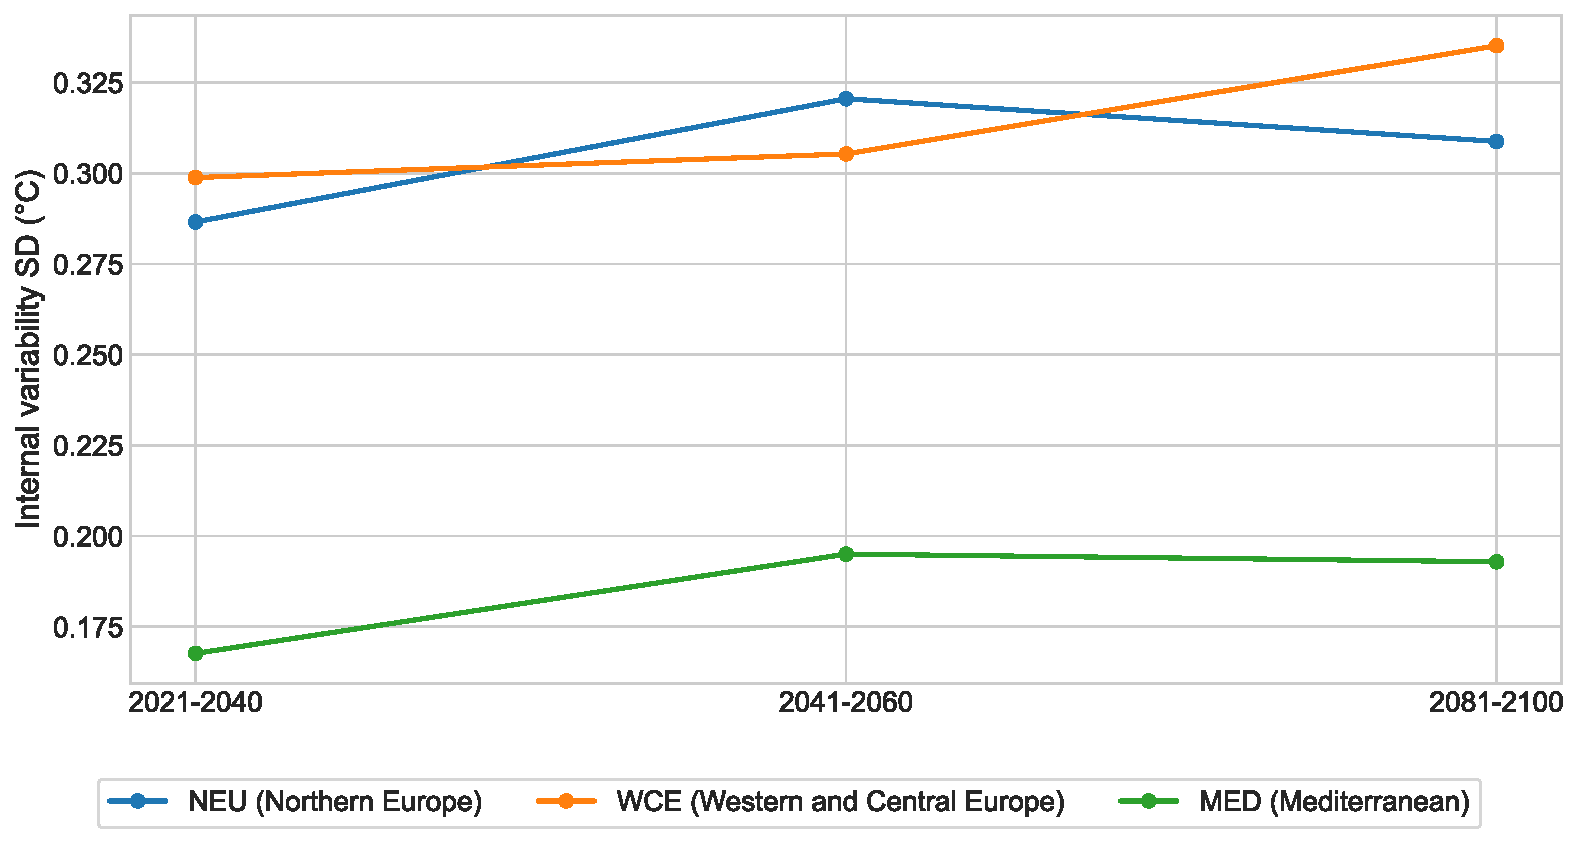
\includegraphics[width=0.7\linewidth]{work/01-climate_uncertainty/figures/fig12_regional_temporal_internal_sd} 

}

\caption{Regional and temporal comparison of internal standard deviation in 20-year mean JJA warming.}\label{fig:unc-appendix-internal-sd}
\end{figure}

\begin{figure}

{\centering 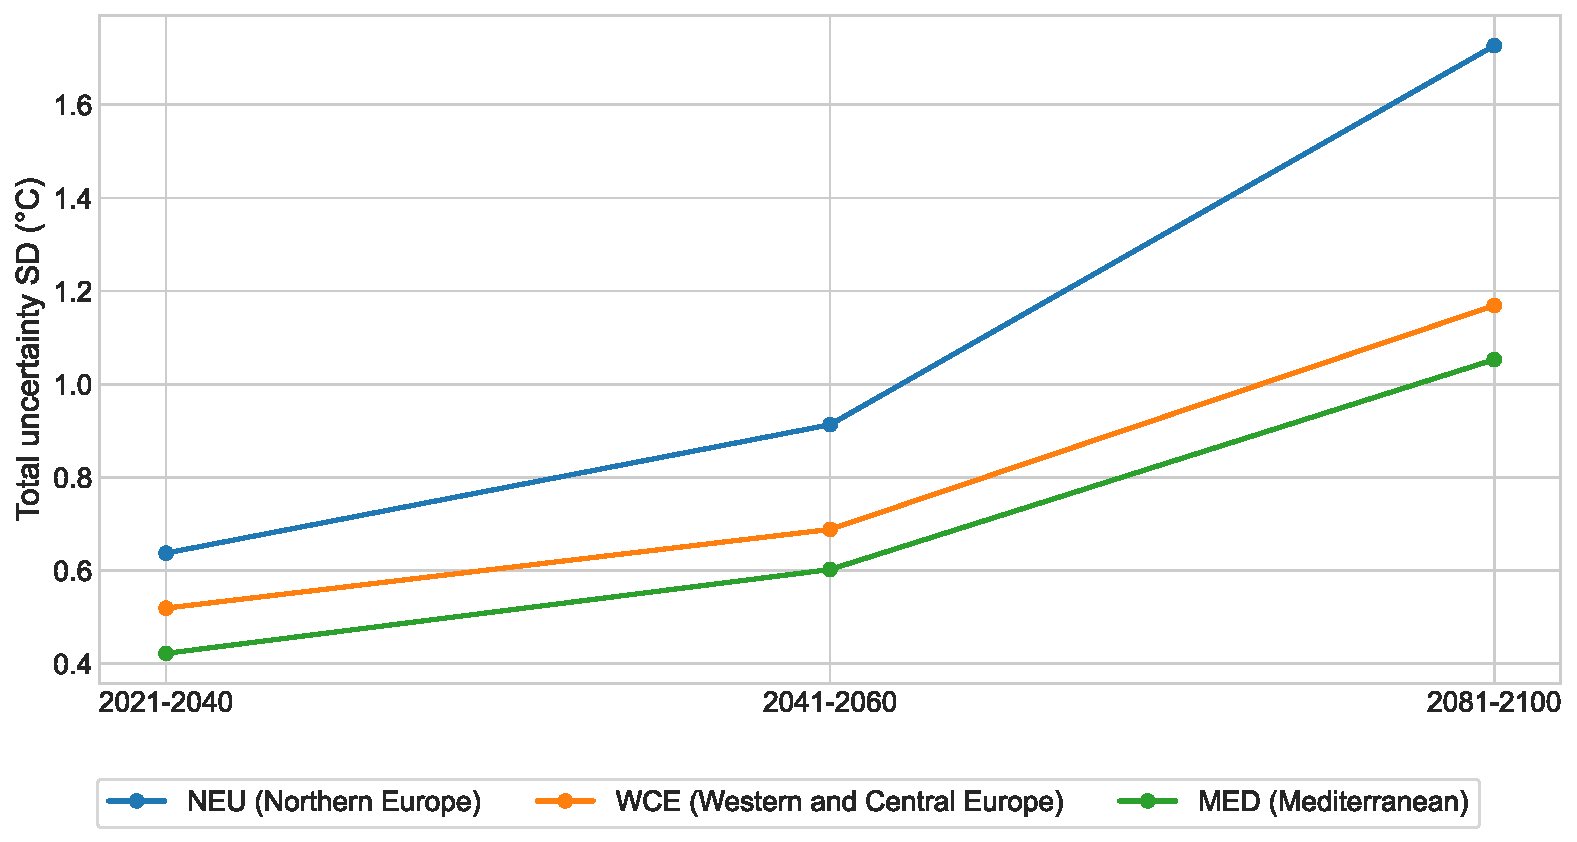
\includegraphics[width=0.7\linewidth]{work/01-climate_uncertainty/figures/fig13_regional_temporal_total_sd} 

}

\caption{Regional and temporal comparison of total fixed-scenario projection standard deviation.}\label{fig:unc-appendix-total-sd}
\end{figure}

\begin{figure}

{\centering 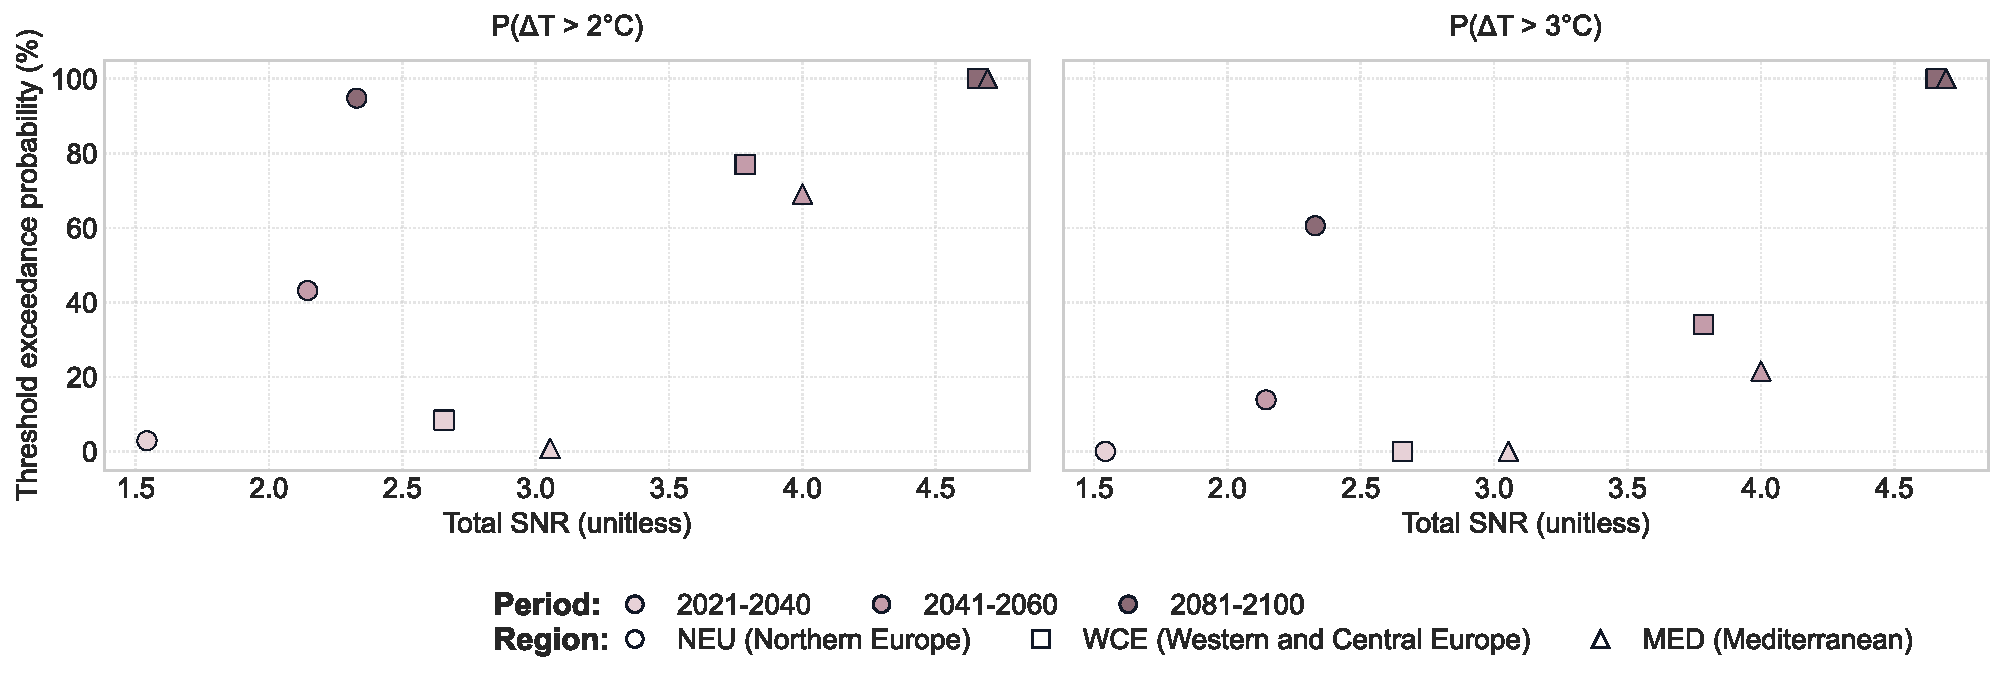
\includegraphics[width=1\linewidth]{work/01-climate_uncertainty/figures/fig15a_threshold_centered_snr_exceedance_probability} 

}

\caption{Relationship between Total SNR and Threshold Exceedance Probability.}\label{fig:unc-appendix-snr-threshold}
\end{figure}

\subsection{Appendix C. Robustness Diagnostics}\label{appendix-c.-robustness-diagnostics}

\textbf{Table C.1. Average width of the 95\% hierarchical-bootstrap percentile interval by metric.}

\begin{table}[!h]
\centering\begingroup\fontsize{10}{12}\selectfont

\resizebox{\ifdim\width>\linewidth\linewidth\else\width\fi}{!}{
\begin{tabular}{lr}
\toprule
Metric & Mean 95\% CI width\\
\midrule
exceedance\_probability\_2c & 0.266\\
exceedance\_probability\_3c & 0.259\\
internal\_contribution & 0.519\\
internal\_sd & 0.124\\
internal\_snr & 8.167\\
\addlinespace
model\_contribution & 0.519\\
total\_sd & 0.629\\
total\_snr & 5.006\\
\bottomrule
\end{tabular}}
\endgroup{}
\end{table}

\textbf{Table C.2. Comparison of full-member and balanced 20-member-per-model estimates for total standard deviation and total signal-to-noise ratio.}

\begin{table}[!h]
\centering\begingroup\fontsize{10}{12}\selectfont

\resizebox{\ifdim\width>\linewidth\linewidth\else\width\fi}{!}{
\begin{tabular}{llrrrr}
\toprule
region & period & Full total SD & Balanced total SD & Full total SNR & Balanced total SNR\\
\midrule
MED & 2021-2040 & 0.422 & 0.423 & 3.054 & 3.050\\
MED & 2041-2060 & 0.602 & 0.601 & 4.000 & 4.013\\
MED & 2081-2100 & 1.053 & 1.054 & 4.694 & 4.691\\
NEU & 2021-2040 & 0.637 & 0.635 & 1.543 & 1.556\\
NEU & 2041-2060 & 0.913 & 0.909 & 2.145 & 2.161\\
\addlinespace
NEU & 2081-2100 & 1.727 & 1.724 & 2.329 & 2.335\\
WCE & 2021-2040 & 0.519 & 0.519 & 2.656 & 2.667\\
WCE & 2041-2060 & 0.688 & 0.685 & 3.785 & 3.809\\
WCE & 2081-2100 & 1.169 & 1.171 & 4.657 & 4.652\\
\bottomrule
\end{tabular}}
\endgroup{}
\end{table}

\chapter{Long-term drought prediction using deep neural networks based on geospatial weather data}\label{dp}

\emph{Author: Helena Veit}

\emph{Supervisor: Henri Funk}

\emph{Degree: Master}

\section{Introduction}\label{introduction-1}

Drought has no single, universally accepted definition, and which definition applies depends on the part of the water cycle and the impacts under consideration \citep{zargar2011}.
Four types are commonly distinguished (Figure \ref{fig:dp-drought-types}, adapted from \citet{nandgude2023}): in a simplified manner a precipitation deficit produces a \emph{meteorological} drought, which depletes soil moisture into an \emph{agricultural} drought, lowers streamflow and groundwater into a \emph{hydrological} drought, and finally reaches water-dependent goods as a \emph{socioeconomic} drought.



\begin{figure}

{\centering 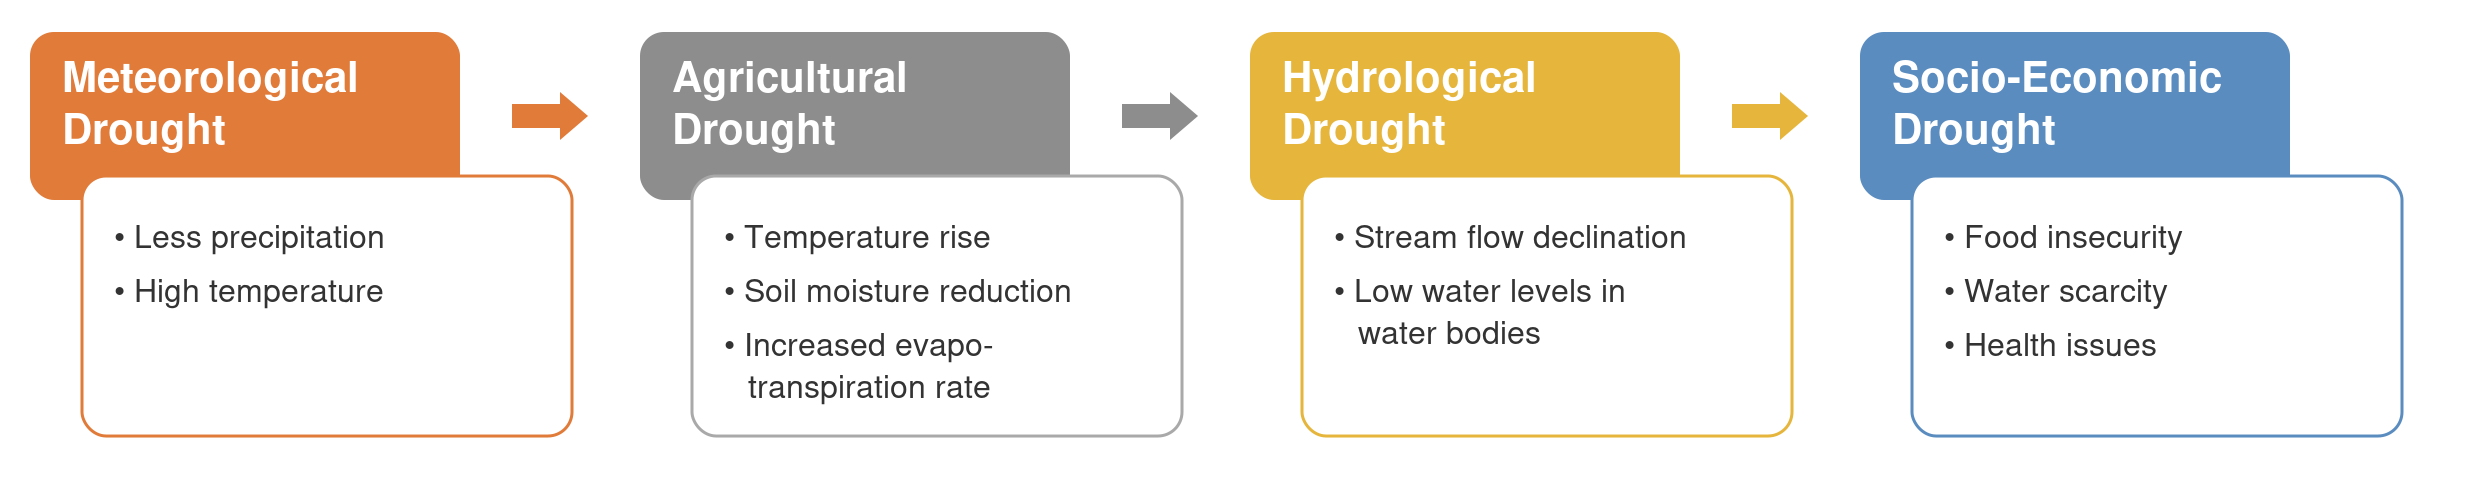
\includegraphics[width=1\linewidth]{work/02-drought_prediction/figures/general/drought_types_vector} 

}

\caption{The four drought types as a propagating cascade. The depiction is adapted from \citet{nandgude2023}.}\label{fig:dp-drought-types}
\end{figure}

This work targets \emph{meteorological drought}, the first stage and earliest signal, driven by a precipitation deficit together with high evapotranspiration.
It can be quantified with various indices, of which this work uses the Standardized Precipitation Evapotranspiration Index (SPEI) \citep{vicenteserrano2010}.

Predicting such droughts well ahead of time is valuable for agriculture, water management, and planning, where early warning shapes what can be done in response.
It is also difficult, since at a lead of several months to a year the predictable signal is weak, and it is further obscured by the rising drought frequency of the last decades.

This work forecasts SPEI-1 over the Alpine region one year into the future from thirty-six months of history, using a convolutional LSTM (ConvLSTM) that treats spatial and temporal structure jointly.
Rather than search for a single best model, it asks which design choices actually shape performance, comparing training losses and how global and static features are supplied to the network.
Three research questions guide this work:

\begin{itemize}
\tightlist
\item
  \textbf{RQ1 (loss):} How does the choice of loss function affect drought detection in a regression setting?
\item
  \textbf{RQ2 (global features):} How can dynamic global features be integrated into the ConvLSTM architecture?
\item
  \textbf{RQ3 (static features):} How can static spatial features be integrated into the ConvLSTM architecture?
\end{itemize}

Answering these questions is the main contribution: a controlled comparison of loss and feature-injection choices for long-term drought prediction.

\section{Related Work}\label{related-work}

Drought prediction has moved from simple baselines such as logistic regression and gradient-boosted trees (see e.g. \citet{marusov2024}) toward machine and deep learning \citep{nandgude2023}.
The task is both temporal, inferring a future drought from past conditions, and spatial, since nearby locations are not independent. Approaches mainly differ in how they handle the two.
Models from the LSTM family capture the temporal side well but treat space only through their inputs or not at all \citep{wang2023, chen2025}, whereas graph-based and transformer models represent the spatial field more directly \citep{yu2023, gao2023, pathak2022, nguyen2023}, at the cost of model scale and compute, and without a guaranteed performance edge, since simple linear baselines can often rival transformer forecasters \citep{zeng2022}.

Across the named studies two factors stand out.
First, they mostly forecast at a short, one-month lead \citep{wang2023, chen2025, yu2023}, the main exception treating long-lead drought as a binary classification \citep{marusov2024}.
Second, evaluation usually falls on one side of a divide, a continuous index scored by average error or discrete categories scored by classification metrics.
The loss function and the handling of input features are usually fixed rather than compared accross different options.

This work directly predicts SPEI-1 at a twelve-month lead over the entire Alpine region, evaluates it for both point accuracy and severe-drought detection skill, and studies how the choice of loss and the injection strategies for global and static features shape the trade-off between them.

\section{Data and Task}\label{data-and-task}

\subsection{Domain and source}\label{domain-and-source}

The study region is the Alpine region at a monthly resolution from 1971 to 2024 (648 months).
The data is derived from the ERA5-Land data set, regridded to a 12kmx12km resolution.
A fixed mask marks the valid Alpine cells, shown outlined against the surrounding European topography in Figure \ref{fig:dp-al-topography-latex}.

\subsection{Variables}\label{variables}

The inputs fall into three groups.

The \emph{dynamic spatial} variables, which vary in both space and time. They include the SPEI (the target, also supplied as history, also seen in Figure \ref{fig:dp-spei-snapshots}), precipitation, near-surface temperature, surface pressure, and water balance.

The \emph{dynamic global} variables, which vary in time only and capture the large-scale drivers of European moisture and its seasonality: the North Atlantic Oscillation index \citep{hurrell1995}, grouped Mediterranean sea-surface temperatures (SST), and a cyclical month encoding.
The fourteen Mediterranean basins are aggregated into three regional means \citep{millot2005, lionello2006} (Figure \ref{fig:dp-med-slt}).

\clearpage
And the \emph{static spatial} input, which varies in space only: the topography, whose elevation strongly shapes Alpine precipitation and temperature.

\begin{figure}[htbp]

{\centering 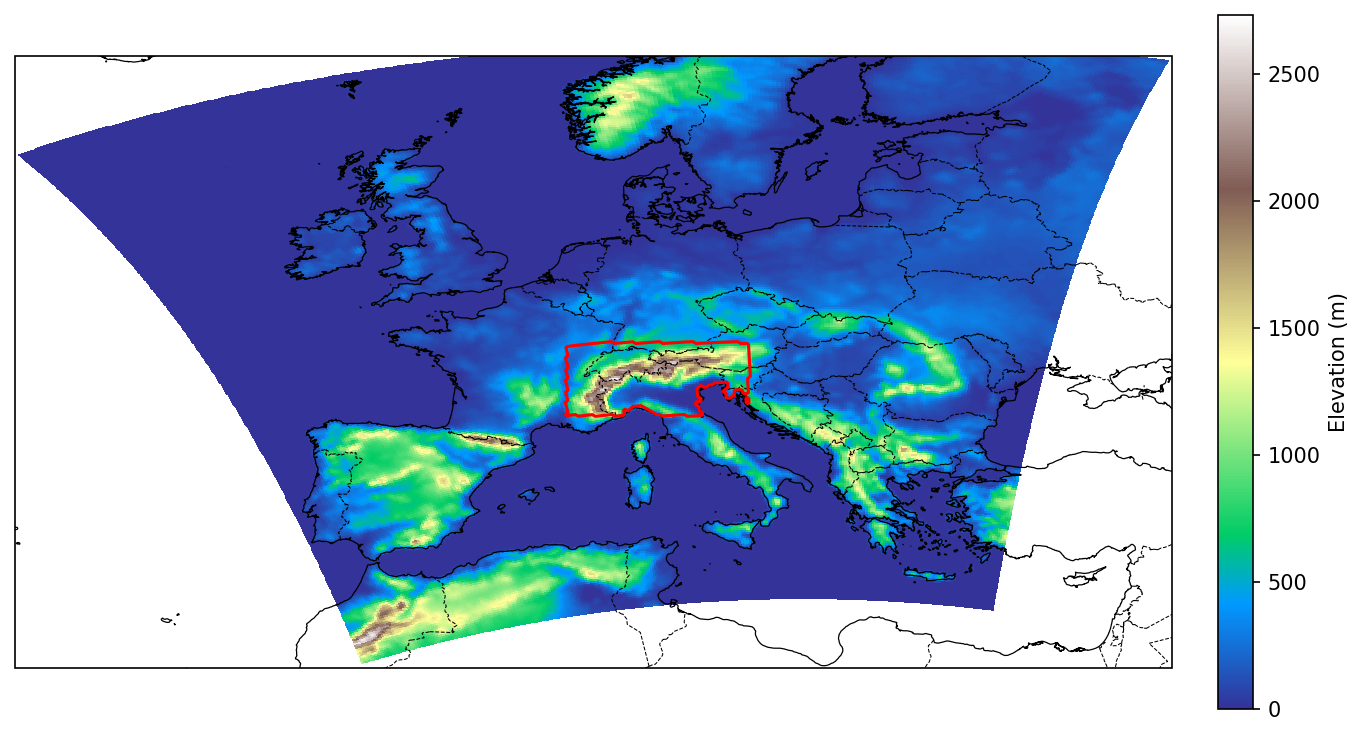
\includegraphics[width=0.7\linewidth]{work/02-drought_prediction/figures/raw/topography} 

}

\caption{Topography over Europe. The red outline marks the Alpine study domain.}\label{fig:dp-al-topography-latex}
\end{figure}

\begin{figure}[htbp]

{\centering 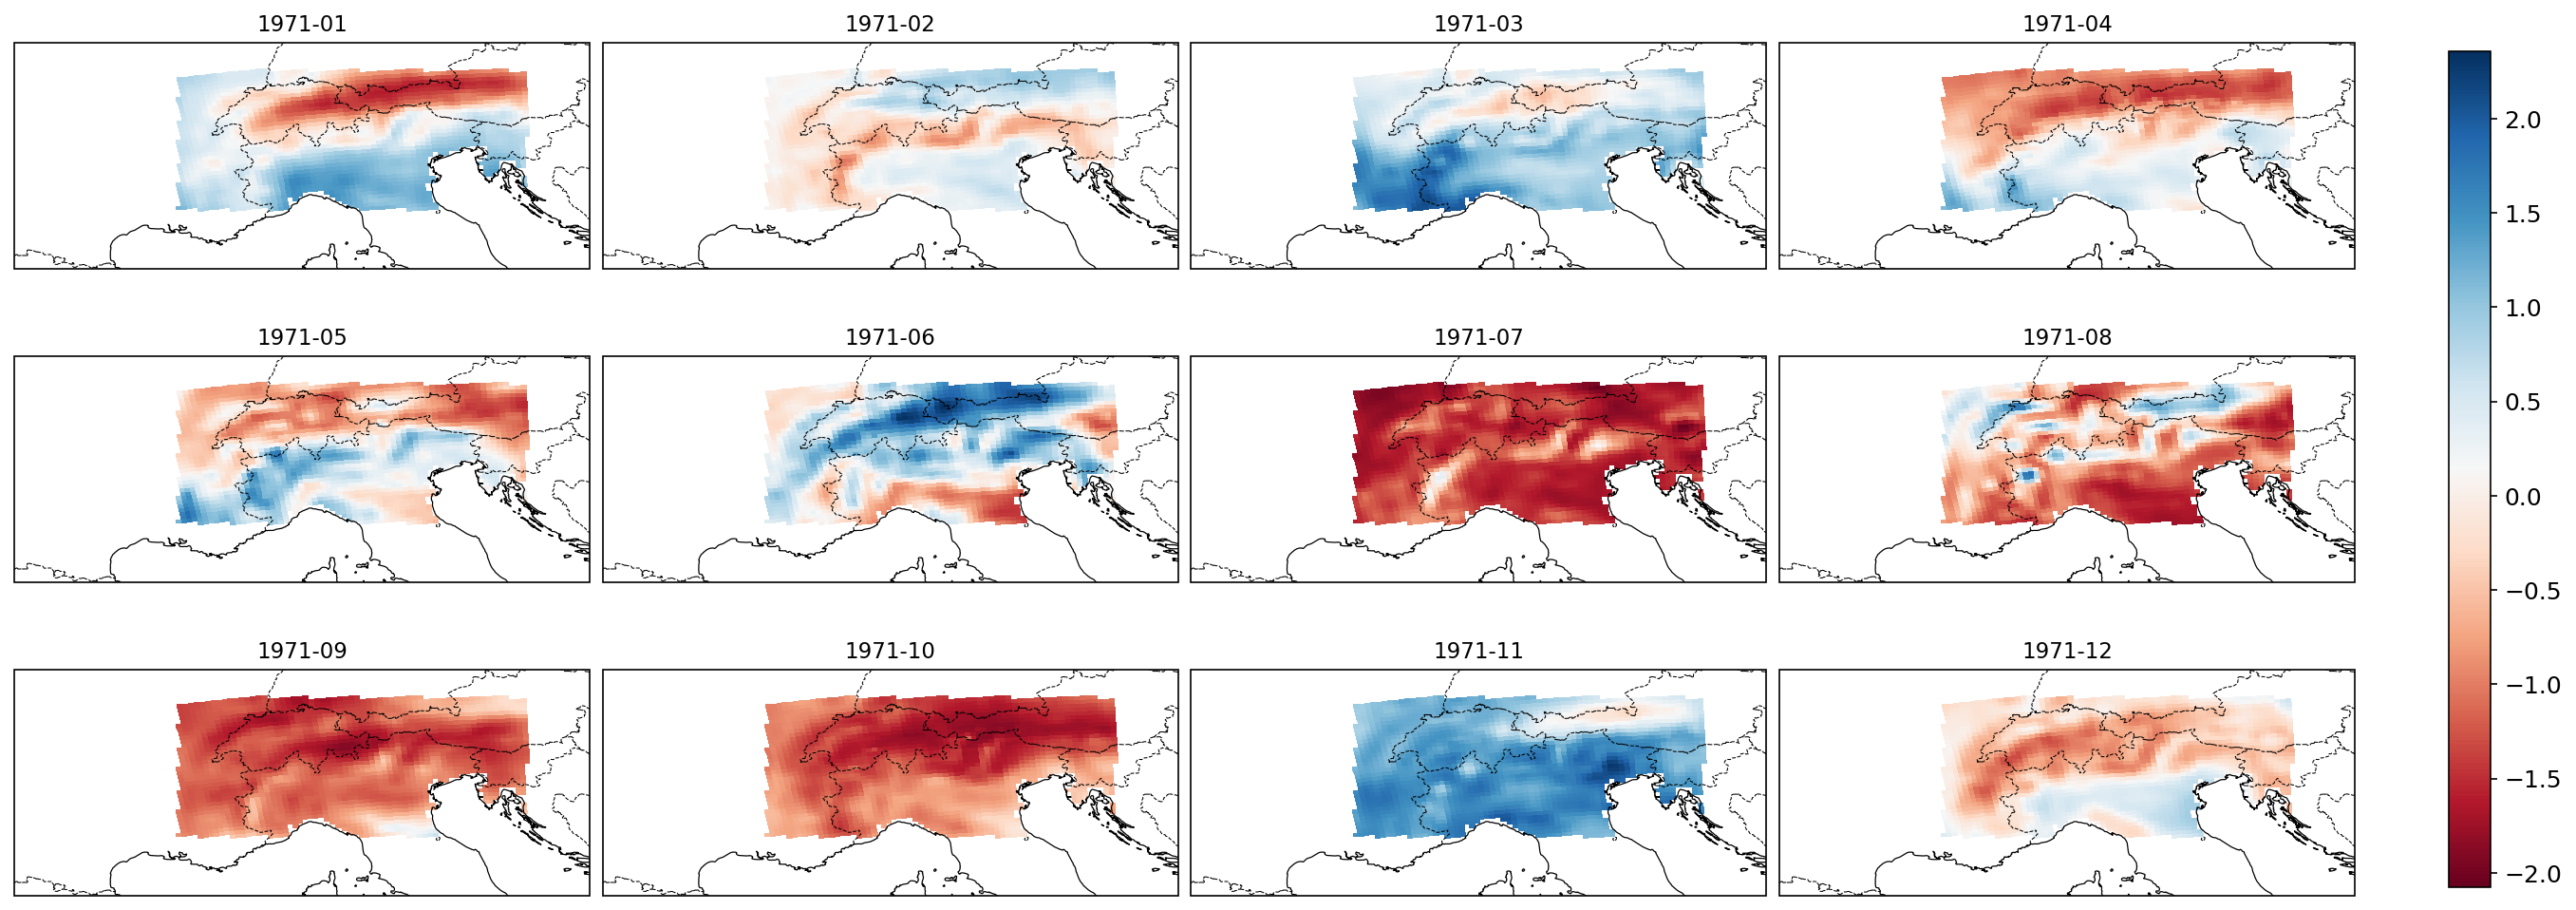
\includegraphics[width=1\linewidth]{work/02-drought_prediction/figures/raw/al/spei} 

}

\caption{SPEI over the Alpine domain across 1971.}\label{fig:dp-spei-snapshots}
\end{figure}

\begin{figure}[htbp]

{\centering 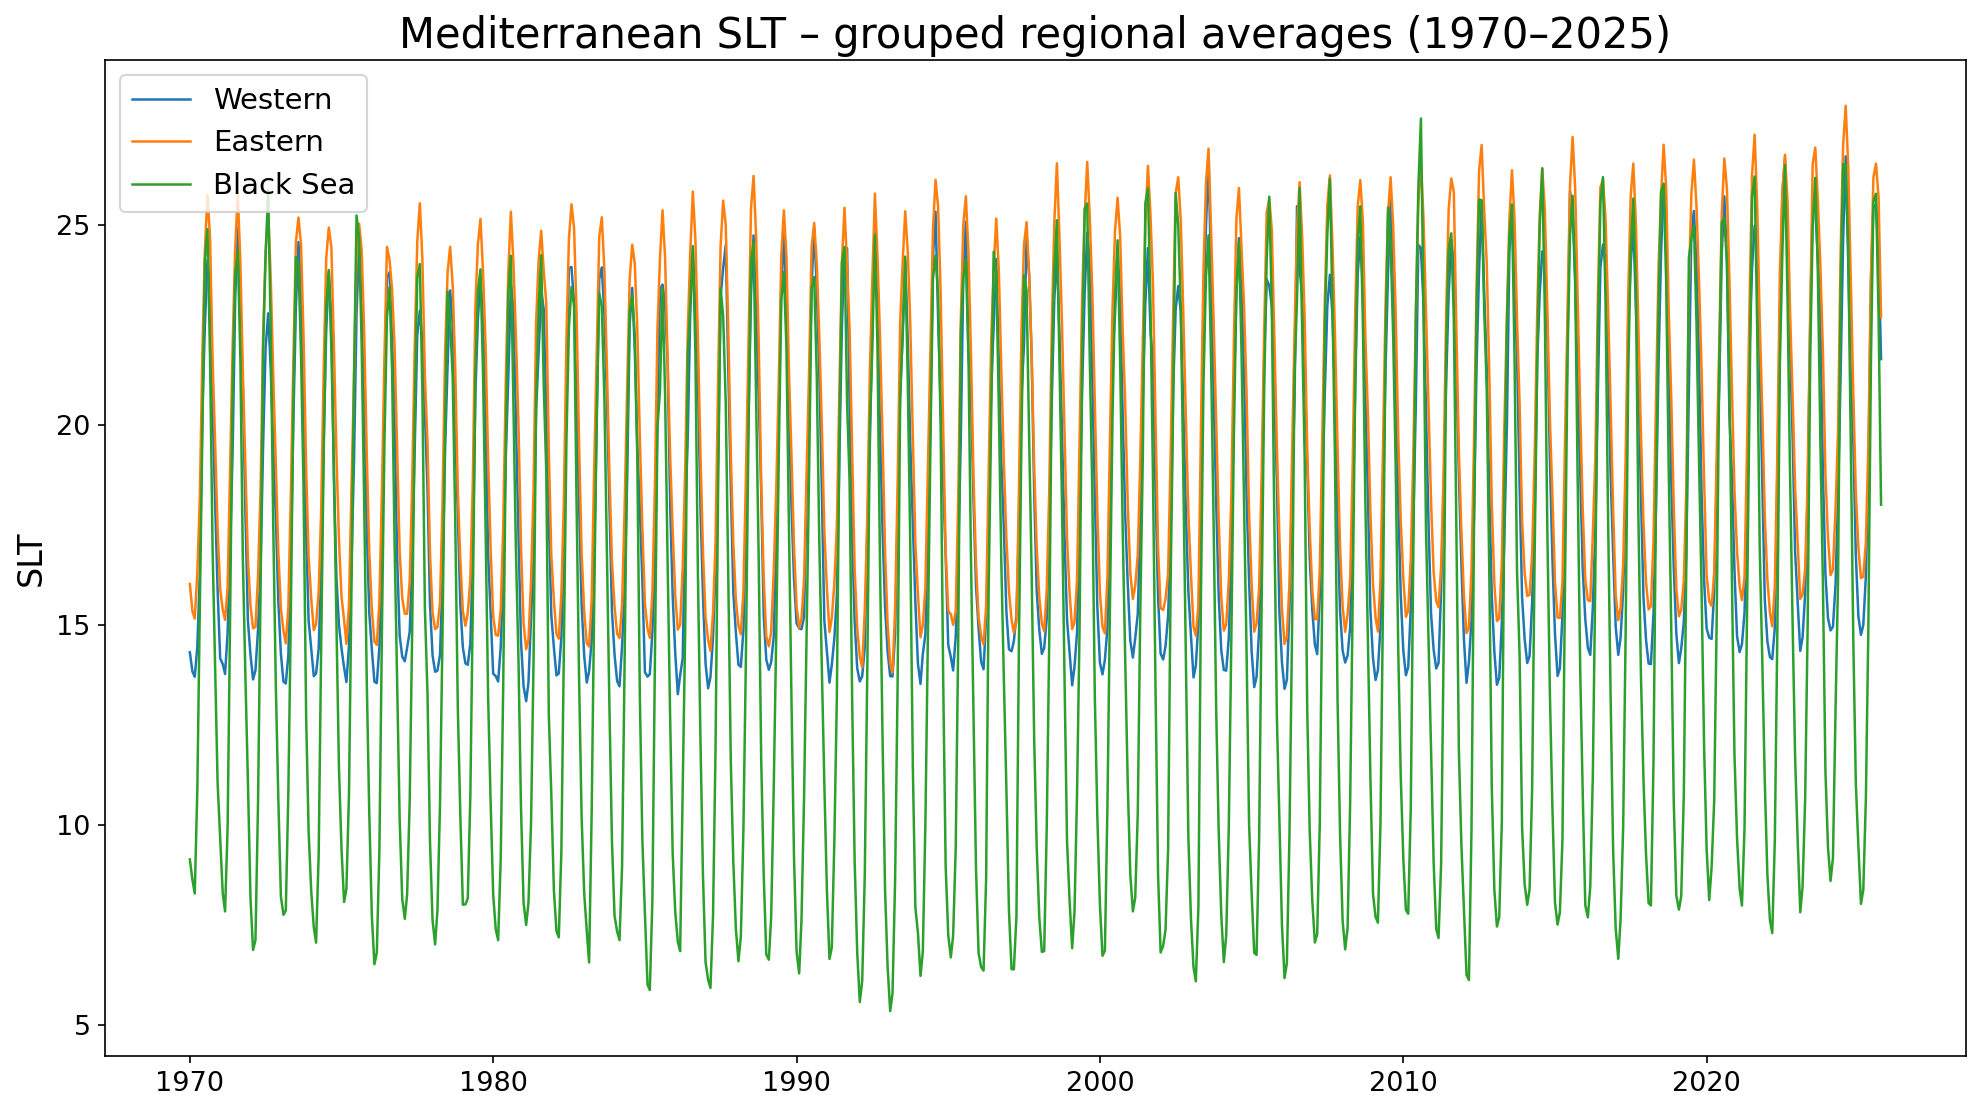
\includegraphics[width=1\linewidth]{work/02-drought_prediction/figures/raw/slides/mediterranean_slt} 

}

\caption{Mediterranean SST, 1971--2024, aggregated into three regional groups (western Mediterranean, eastern Mediterranean, Black Sea).}\label{fig:dp-med-slt}
\end{figure}

\clearpage

\subsection{Drought definition: SPEI}\label{drought-definition-spei}

The Standardized Precipitation Evapotranspiration Index (SPEI) \citep{vicenteserrano2010} extends the precipitation-only Standardized Precipitation Index (SPI) \citep{mckee1993} by using the water balance, so that temperature enters through evapotranspiration, which can better account for rising temperatures under climate change.

The SPEI is built on the water balance,

\[D = P - PET, \qquad \begin{cases} D > 0 & \text{water surplus} \\ D < 0 & \text{water deficit} \end{cases}\]

where \(P\) is precipitation and \(PET\) is potential evapotranspiration.

SPEI is defined at a chosen timescale \(k\): the monthly water balance is summed over a rolling window of the preceding \(k\) months, and the accumulated series is fitted to a distribution and standardized.
Common choices are 1, 3, 6, 12, and 24 months.
Short timescales respond to rapid, month-to-month deficits and longer ones to slower, accumulated dryness.
This work uses SPEI-1, so each value uses the water balance of one month expressed in standard deviations from the local mean.
The index is computed as in \citet{funk2026}, with a three-parameter gamma fit calibrated over 1990 to 2019.

\subsection{Preprocessing}\label{preprocessing}

Cells outside the Alpine mask are filled and excluded from all statistics.
All variables, including SPEI, are standardized to zero mean and unit variance using training-years statistics over valid cells only.
Because SPEI is also the prediction target, this same training-period standardization sets the units of the target, so predictions, the reported RMSE, and the SPEI \(\le -1.5\) detection threshold are all expressed in training-period standardized units.

\subsection{Split and nonstationarity}\label{split-and-nonstationarity}

The data is split chronologically: training on 1971 to 2004, validation on 2005 to 2014, and testing on 2015 to 2024.
Because the split is by time rather than at random, the periods differ in climate.
The average severe-drought frequency rises across them, from 0.53 to 0.62 to 1.04 events per cell per year, so the test period is substancially drier than the training period, as shown in Figure \ref{fig:dp-drought-freq-severe}.

\begin{figure}

{\centering 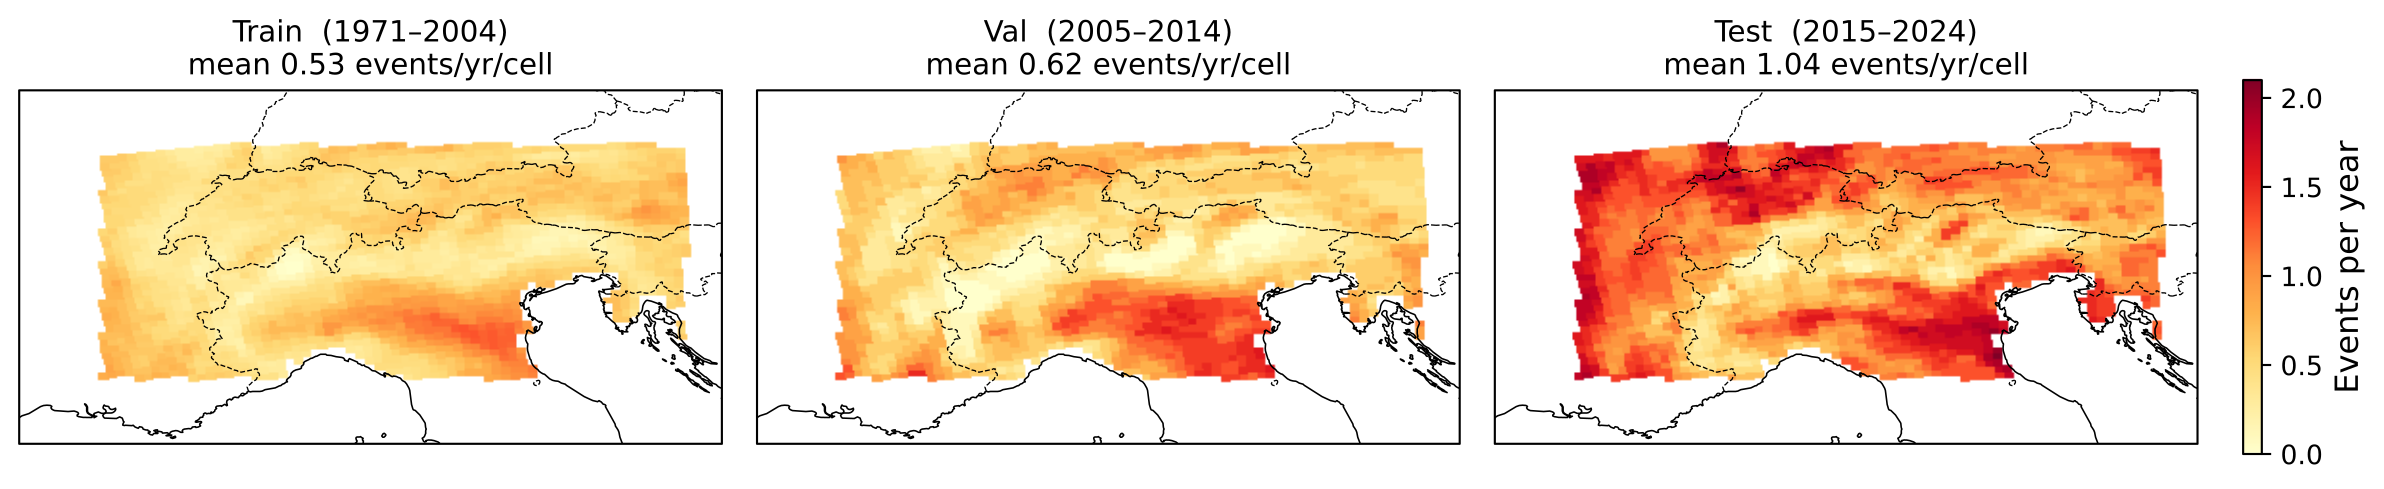
\includegraphics[width=1\linewidth]{work/02-drought_prediction/figures/processed/exploratory/drought_frequency_severe} 

}

\caption{Severe-drought (SPEI $\le -1.5$) frequency by split.}\label{fig:dp-drought-freq-severe}
\end{figure}

\subsection{Task \& Model}\label{task-model}

The forecasting task is a continuous, per-cell regression of SPEI-1.
Given thirty-six months of history, the model predicts a single SPEI-1 map at a twelve-month lead.
It is a direct forecast, the horizon is predicted in one step rather than iterated month by month, avoiding recursive error accumulation.

The forecasting model is a Convolutional LSTM (ConvLSTM), following the variant of \citet{marusov2024}.
It replaces the matrix products in the gates of a standard LSTM \citep{hochreiter1997} with convolutions, so the input \(x_t\), hidden state \(h_t\), and cell state \(c_t\) are three-dimensional feature maps rather than vectors, which preserves spatial structure.
Figure \ref{fig:dp-convlstm-schematic} shows the resulting cell.



\begin{figure}[htbp]

{\centering 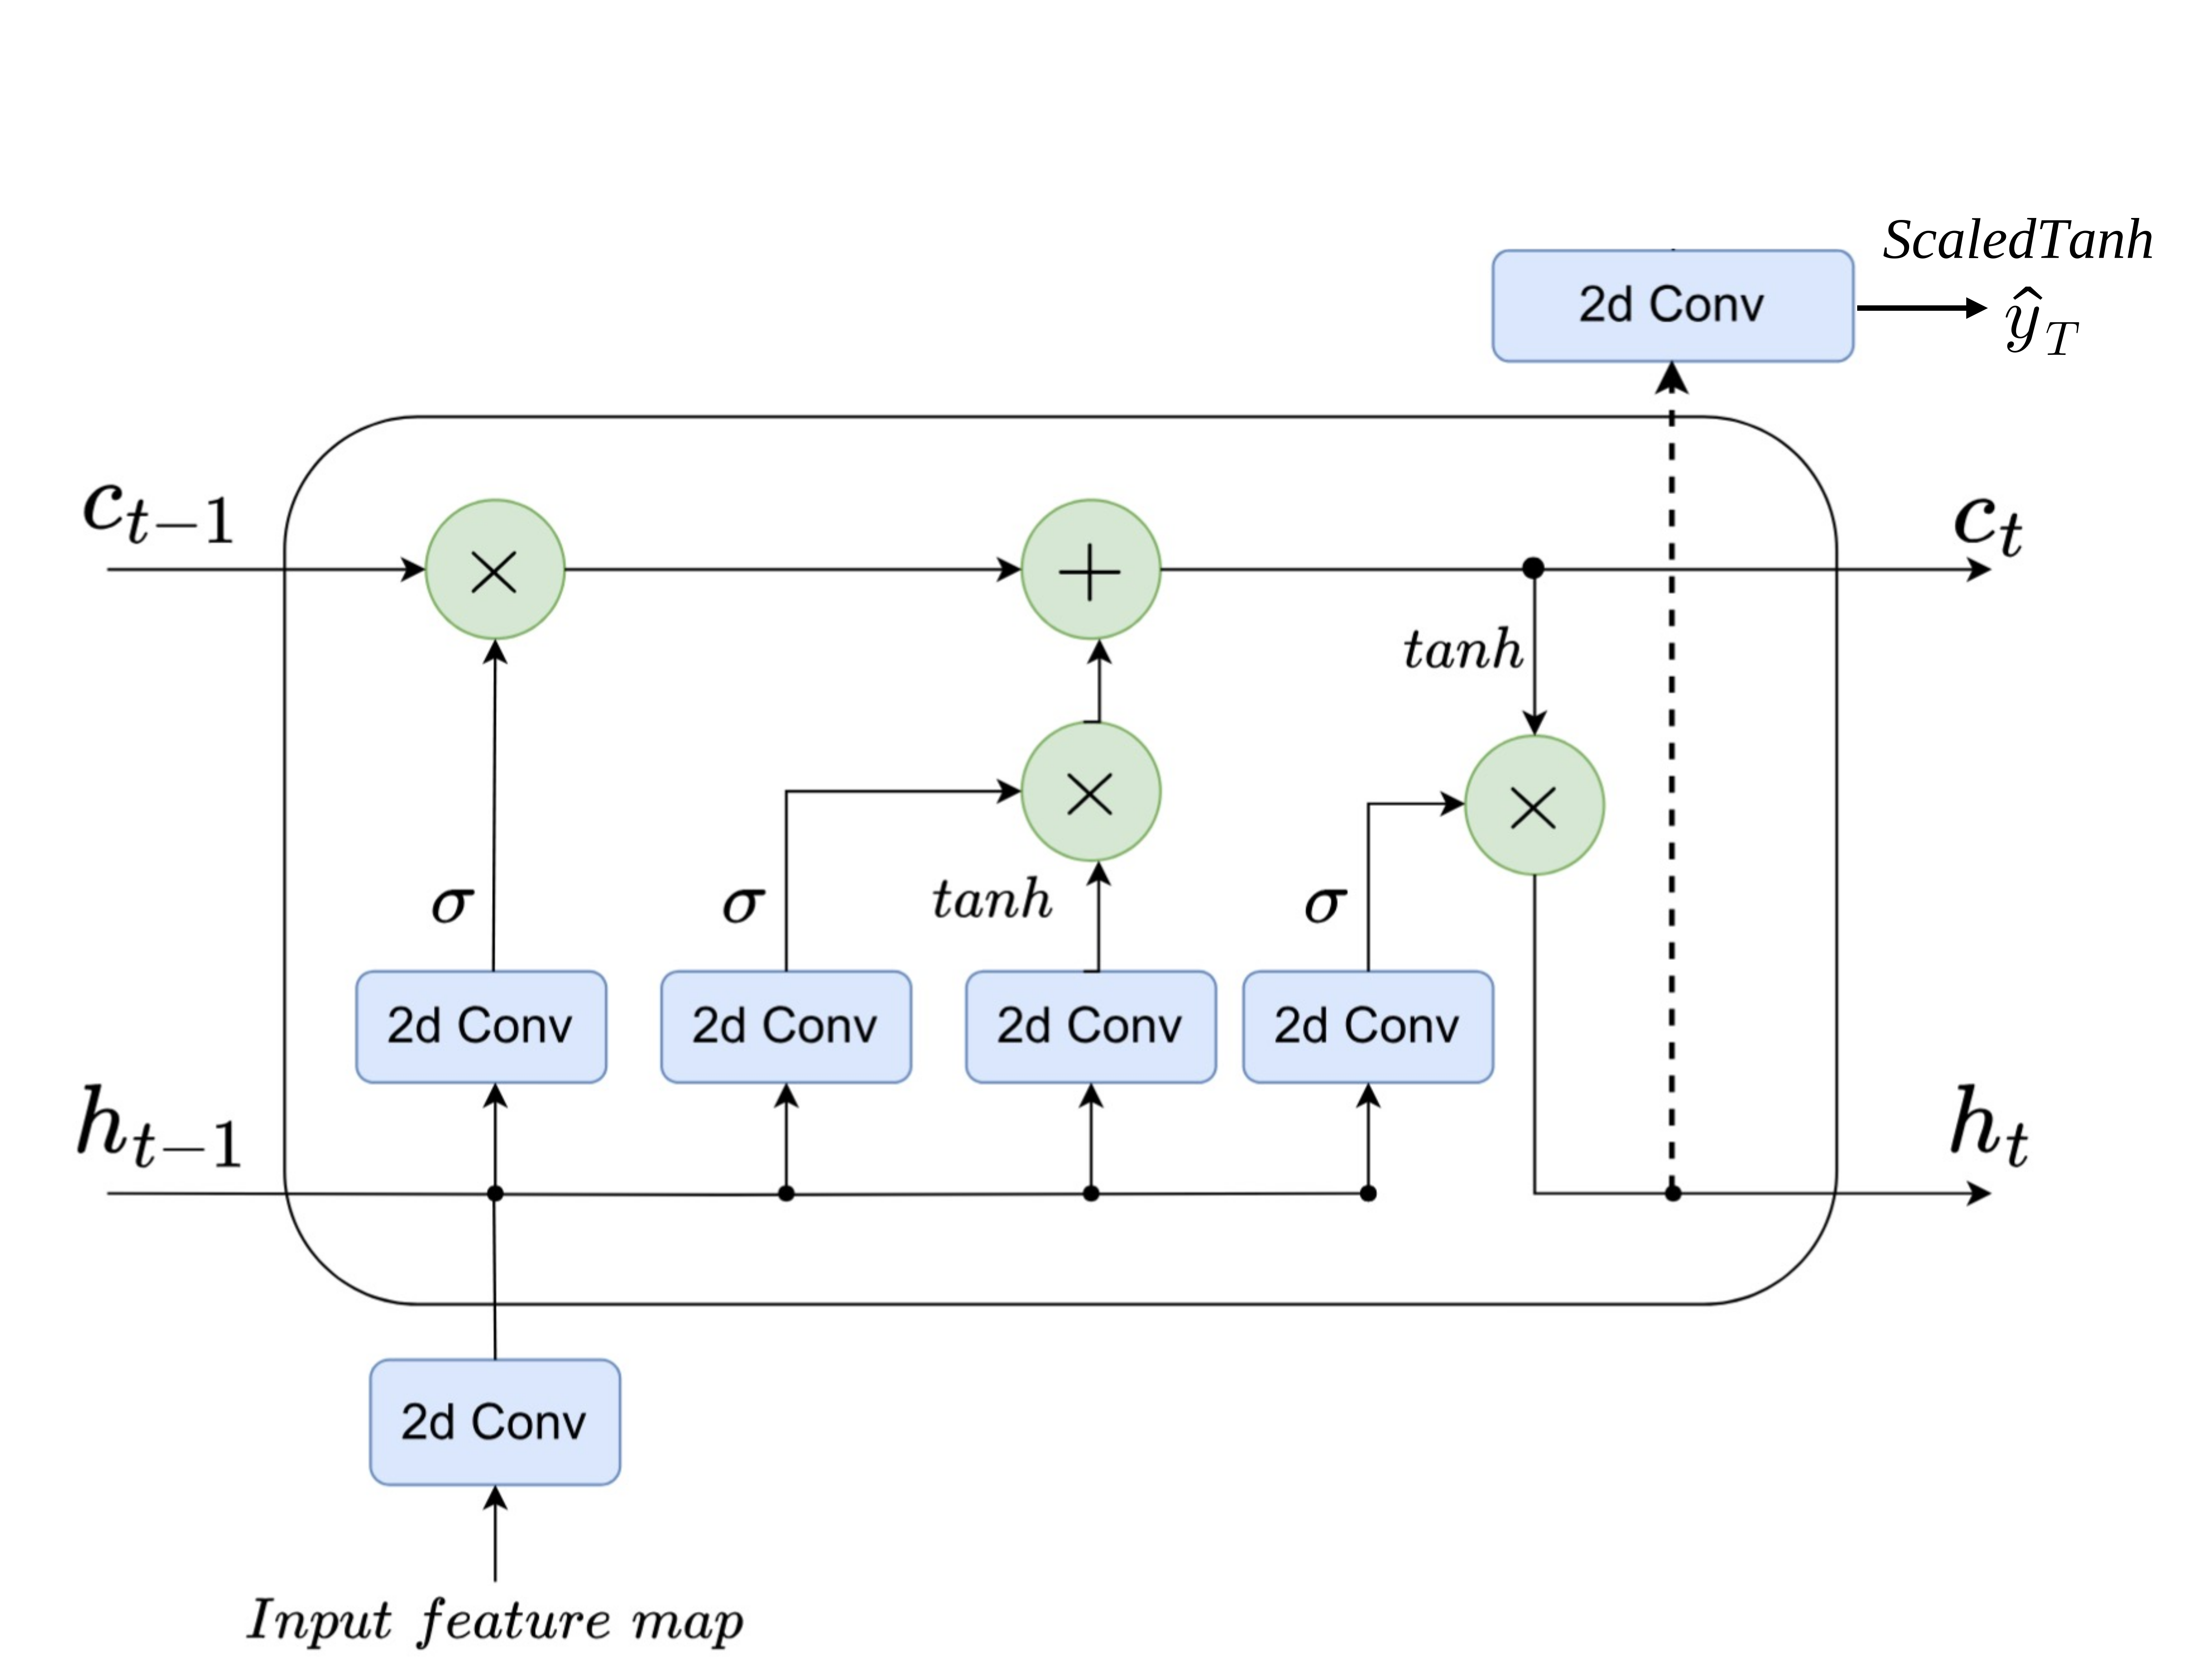
\includegraphics[width=0.75\linewidth]{work/02-drought_prediction/figures/architecture/ConvLSTM} 

}

\caption{ConvLSTM cell. The depiction is by \citet{marusov2024}.}\label{fig:dp-convlstm-schematic}
\end{figure}

Each gate applies a convolution followed by batch normalization, whose affine shift replaces the additive bias,

\[
\begin{aligned}
f_t &= \sigma(\mathrm{BN}(W_f \ast x_t + U_f \ast h_{t-1})), & i_t &= \sigma(\mathrm{BN}(W_i \ast x_t + U_i \ast h_{t-1})), \\
\tilde{c}_t &= \tanh(\mathrm{BN}(W_c \ast x_t + U_c \ast h_{t-1})), & o_t &= \sigma(\mathrm{BN}(W_o \ast x_t + U_o \ast h_{t-1})),
\end{aligned}
\]

and the cell and hidden states are updated as

\[c_t = f_t \odot c_{t-1} + i_t \odot \tilde{c}_t, \qquad h_t = o_t \odot \tanh(c_t),\]

where \(\ast\) denotes convolution, \(\odot\) the elementwise product, and \(\sigma\) the sigmoid.

The final hidden state is mapped to the predicted SPEI map by a bounded regression head,

\[\hat{y}_T = \lambda \tanh(W_{\text{out}} \ast h_T),\]

where the scaled \(\tanh\) keeps the output within \([-\lambda, \lambda]\), with \(\lambda = 10\).

\section{Methods}\label{methods-1}

Each of the three research questions is treated as one axis of variation, as defined below.

\subsection{RQ1: Loss functions}\label{rq1-loss-functions}

The loss sets how strongly errors on dry cells are weighted, and how hard the model is pushed to predict droughts.
Three families are compared, each averaged over valid cells, with \(y\) the observed and \(\hat{y}\) the predicted SPEI.

\textbf{\textcolor[HTML]{3C3C3C}{Mean squared error}} is the symmetric baseline,

\[\mathcal{L}_{\text{MSE}} = (\hat{y} - y)^2.\]

\begin{center}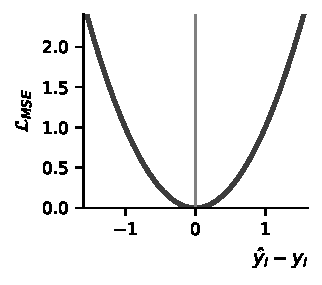
\includegraphics[width=0.33\linewidth]{work/02-drought_prediction/reports/figures/mse} \end{center}

\textbf{\textcolor[HTML]{286EA0}{Hinge-weighted MSE}} keeps the squared error but up-weights cells on the dry side of normal,

\[\begin{aligned}
\mathcal{L}_{\text{hwMSE}} &= w\,(\hat{y} - y)^2, \\
w &= 1 + \alpha \max(0, -y), \quad \alpha \in \{1, 5\},
\end{aligned}\]

so a given error costs more the drier the observed cell.

\begin{center}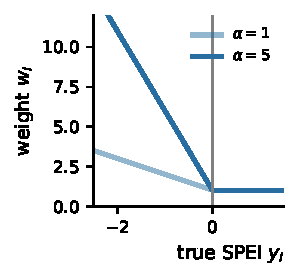
\includegraphics[width=0.33\linewidth]{work/02-drought_prediction/reports/figures/hinge_weight} 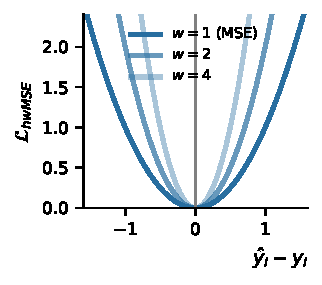
\includegraphics[width=0.33\linewidth]{work/02-drought_prediction/reports/figures/hinge_loss} \end{center}

\textbf{\textcolor[HTML]{C6402A}{Pinball (quantile) loss}} at \(\tau = 0.20\) is asymmetric,

\[\mathcal{L}_{\text{pin}} = \begin{cases} \tau\,(y - \hat{y}) & \hat{y} \le y, \\ (1-\tau)\,(\hat{y} - y) & \hat{y} > y, \end{cases}\]

penalizing over-prediction (too wet, missing a drought) by a factor \(\tfrac{1-\tau}{\tau}=4\) over under-prediction, biasing the model toward the dry tail.

\begin{center}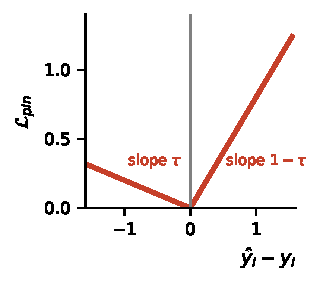
\includegraphics[width=0.33\linewidth]{work/02-drought_prediction/reports/figures/pinball} \end{center}

\subsection{RQ2: Dynamic global features}\label{rq2-dynamic-global-features}

Two ways of feeding the global features into the ConvLSTM are compared (Figure \ref{fig:dp-naive-vs-film}).
The naive baseline broadcasts each global scalar across the grid as an extra input channel.



\begin{figure}[htbp]

{\centering 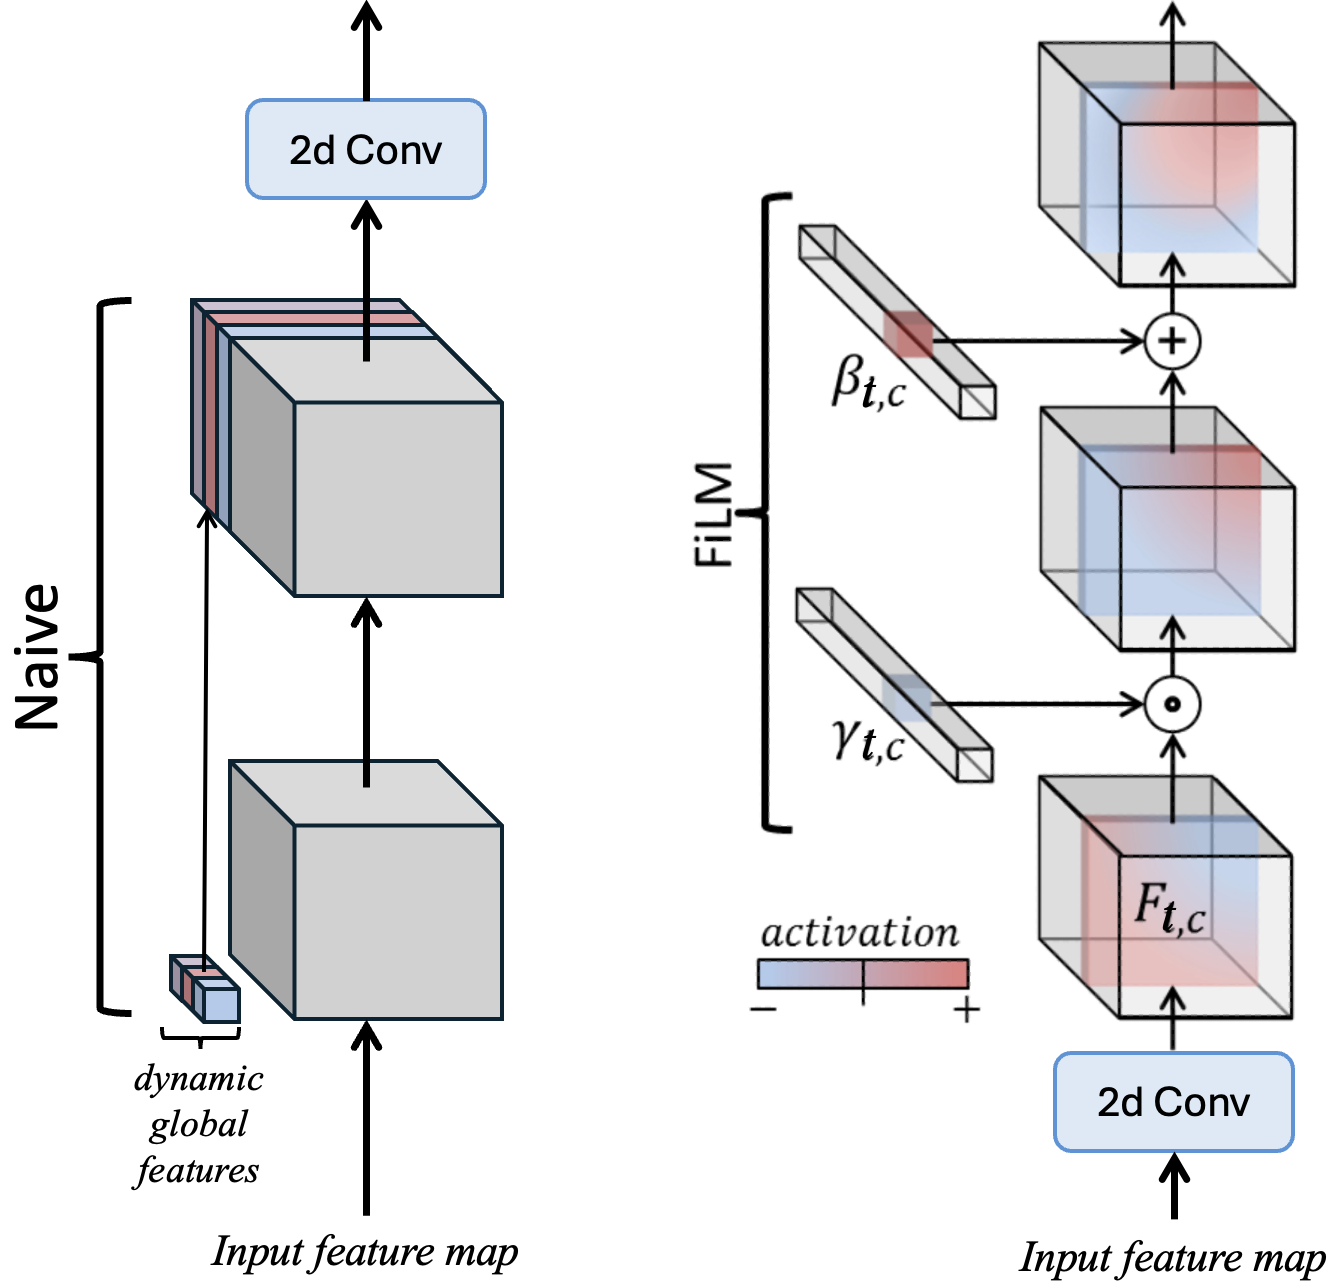
\includegraphics[width=0.6\linewidth]{work/02-drought_prediction/figures/architecture/Naive_vs_film} 

}

\caption{Dynamic global feature injection strategies. Naive injection is on the left and FiLM on the right. The FiLM depiction is by \citet{perez2018}.}\label{fig:dp-naive-vs-film}
\end{figure}

FiLM (feature-wise linear modulation) \citep{perez2018} instead conditions the network by applying a per-channel affine transform to the feature maps,

\[\mathrm{FiLM}(F_c) = \gamma_c\, F_c + \beta_c, \qquad \gamma_c = f_c(x_t), \; \beta_c = h_c(x_t),\]

where \(F_c\) is the activation of channel \(c\) and the scale \(\gamma_c\) and shift \(\beta_c\) are learned functions \(f_c, h_c\) of the global features \(x_t\), produced together by a small shared MLP.
Rather than adding channels, FiLM lets the global state reshape the existing ones in an interaction-like manner. Figure \ref{fig:dp-convlstm-film} shows where this conditioning enters the ConvLSTM cell introduced above.



\begin{figure}[htbp]

{\centering 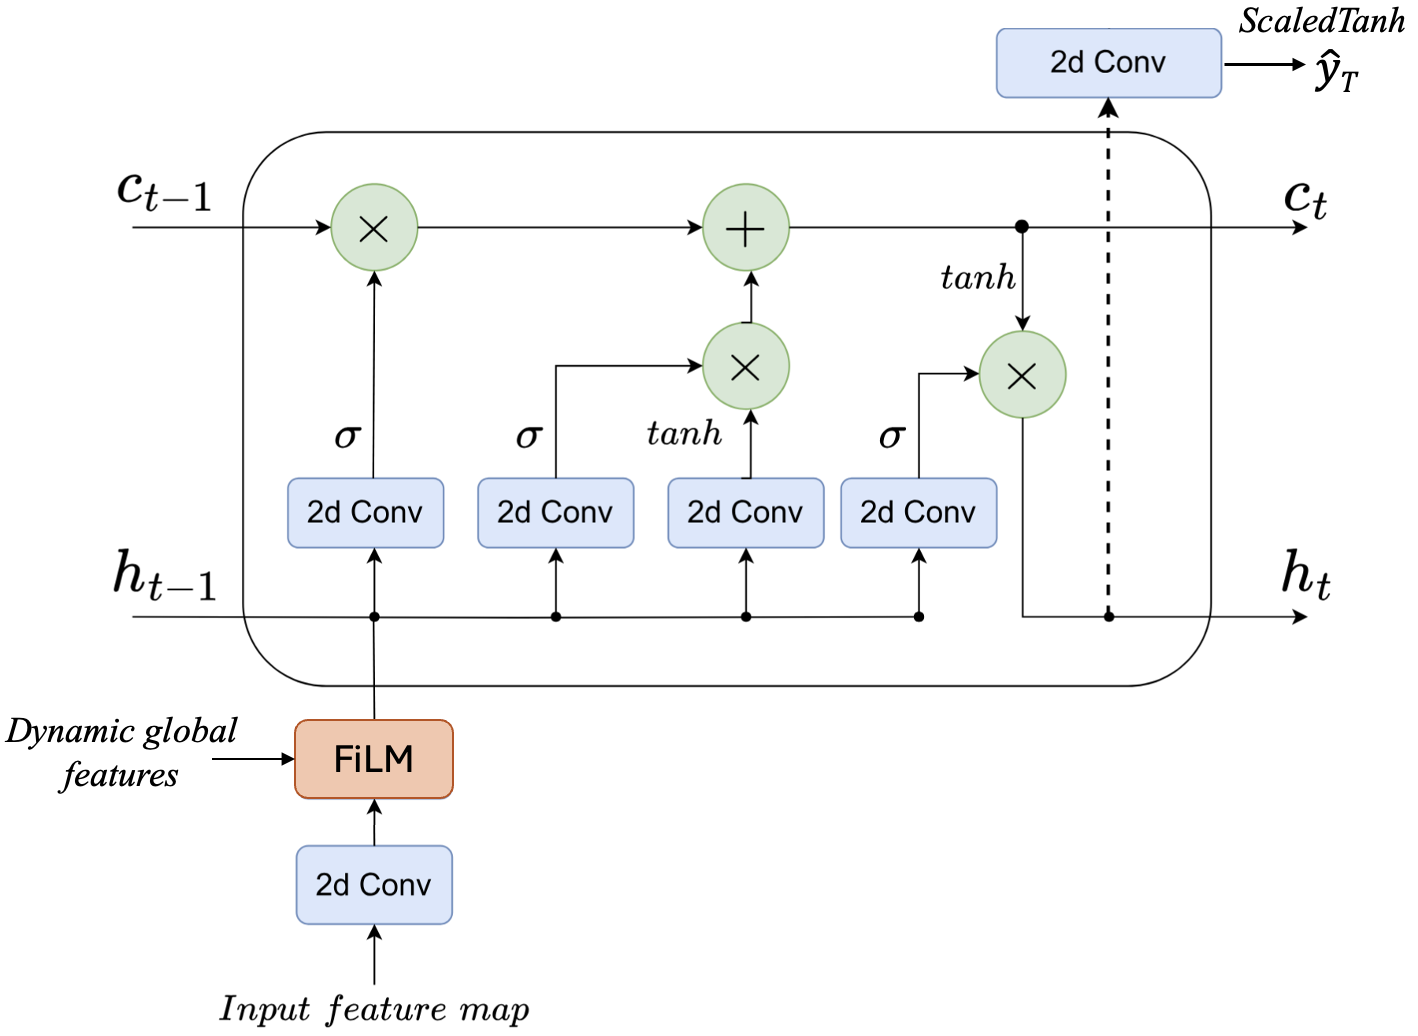
\includegraphics[width=0.75\linewidth]{work/02-drought_prediction/figures/architecture/ConvLSTM_FiLM} 

}

\caption{Where FiLM sits inside the ConvLSTM cell: it conditions the embedded input feature map before the gate convolutions. The ConvLSTM cell depiction is by \citet{marusov2024}.}\label{fig:dp-convlstm-film}
\end{figure}

\clearpage

\subsection{RQ3: Static spatial features}\label{rq3-static-spatial-features}

Three ways of incorporating the static topography are compared, contrasted in Figure \ref{fig:dp-naive-vs-static-encoder}.
The naive baseline appends the raw static field repeatedly at each time step, treating it the same as a dynamic spatial feature.

\begin{figure}[htbp]

{\centering 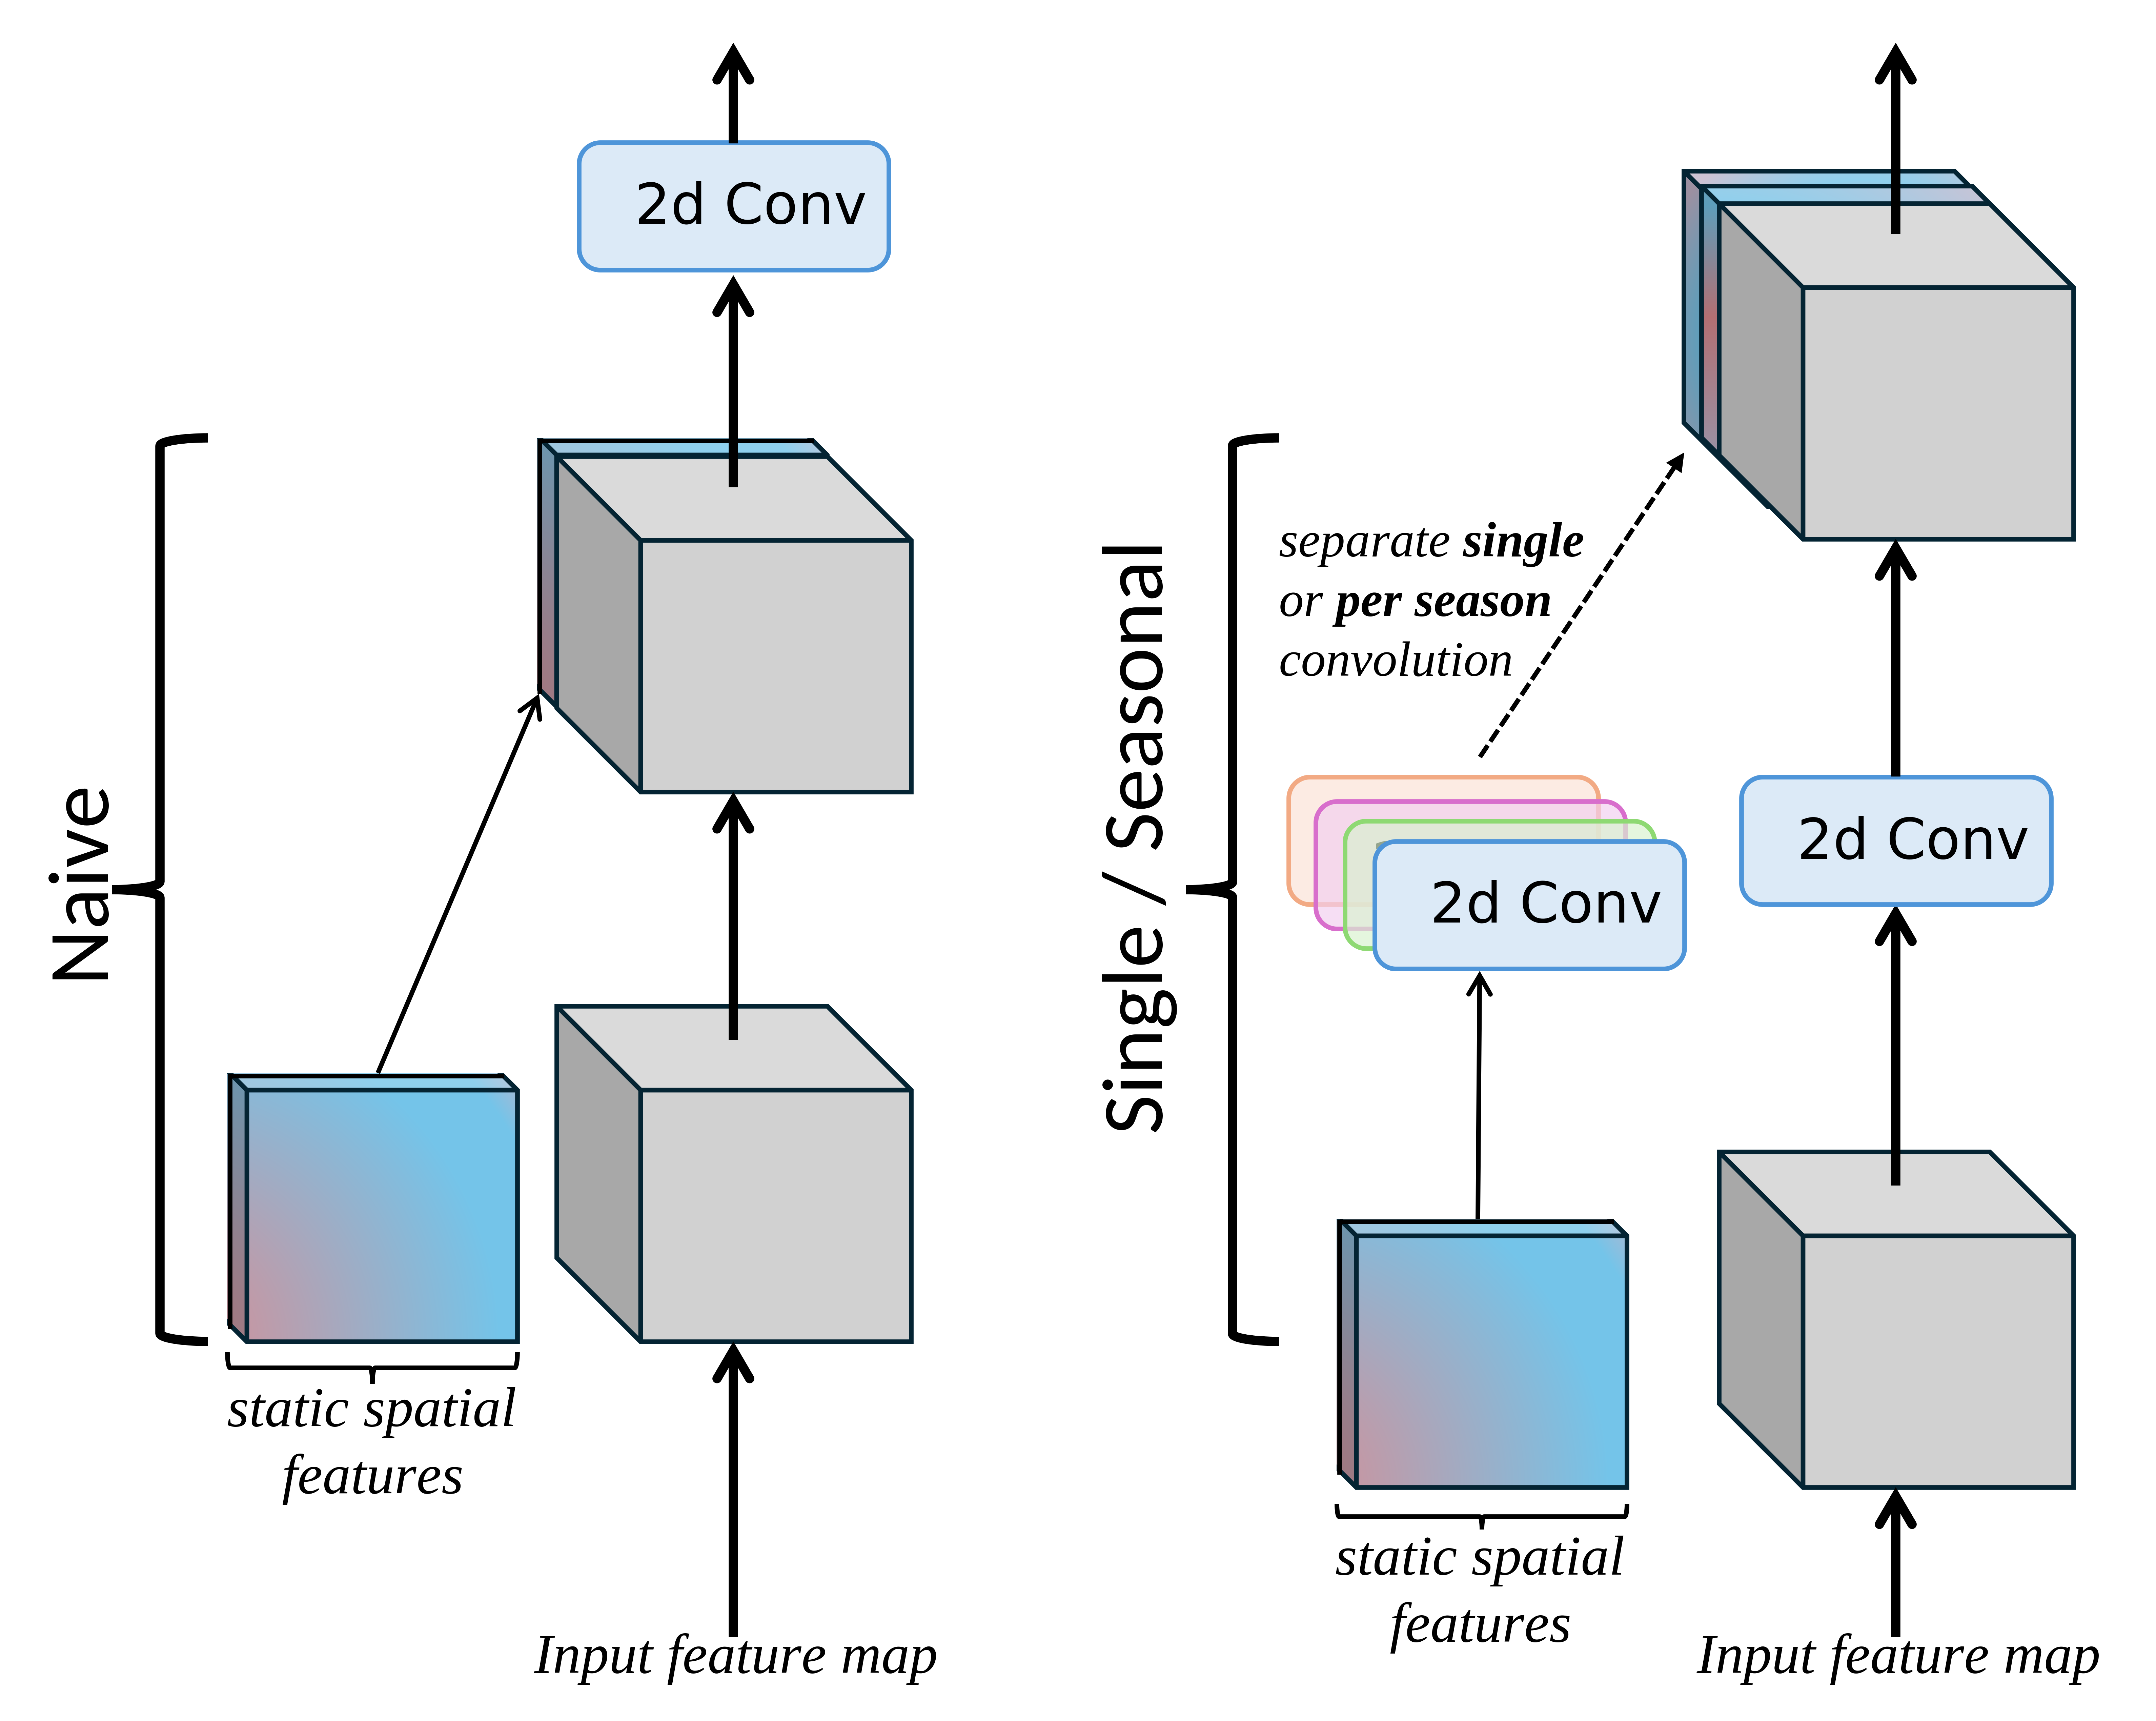
\includegraphics[width=0.6\linewidth]{work/02-drought_prediction/figures/architecture/Naive_vs_single_seasonal} 

}

\caption{Static spatial feature injection strategies. Naive injection is on the left and the learned encoder on the right (single and seasonal variants).}\label{fig:dp-naive-vs-static-encoder}
\end{figure}

The other two learn a seperate static encoding through a small convolutional network,

\[E(S) = \mathrm{ReLU}(W_2 \ast \mathrm{ReLU}(W_1 \ast S)),\]

with static features \(S\) and convolutional kernels \(W_1, W_2\) (each with batch normalization), whose output is concatenated to the embedding \(x_t^{\text{emb}}\) at every timestep.
The \emph{single} variant uses one shared encoder, giving \([\,x_t^{\text{emb}}, E(S)\,]\), while the \emph{seasonal} variant uses four encoders, one per meteorological season, selected by the season \(s(m_t)\) of the target month, giving \([\,x_t^{\text{emb}}, E_{s(m_t)}(S)\,]\). Figure \ref{fig:dp-convlstm-static} shows where the resulting encoder output enters the cell.



\begin{figure}[htbp]

{\centering 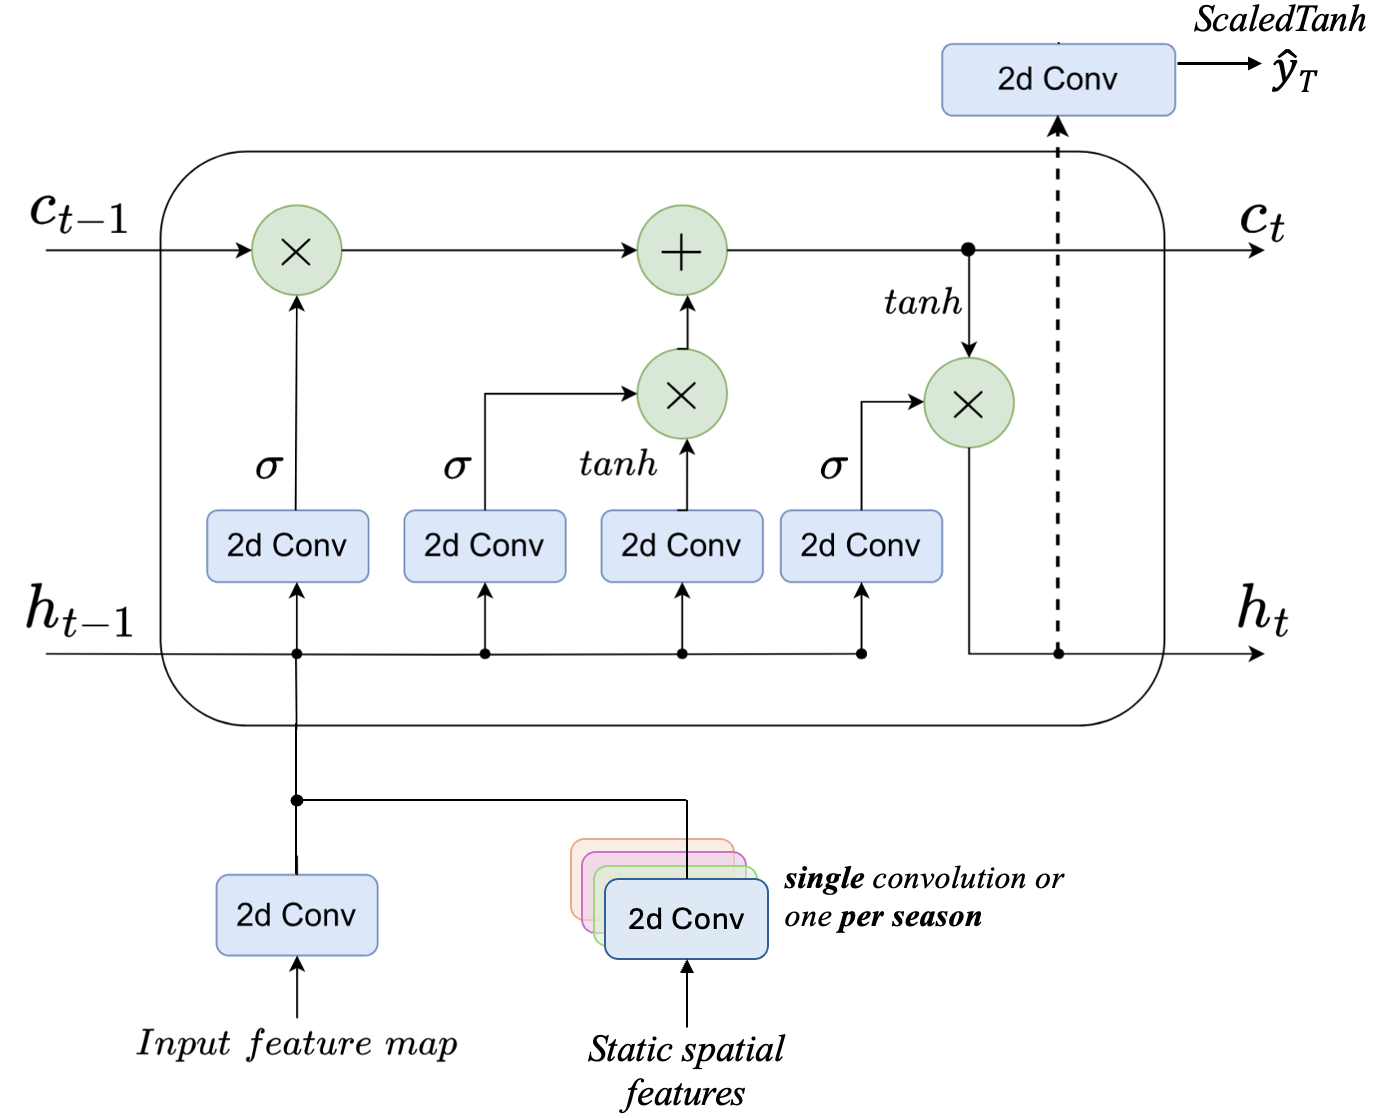
\includegraphics[width=0.75\linewidth]{work/02-drought_prediction/figures/architecture/ConvLSTM_static} 

}

\caption{Where the static encoder sits inside the ConvLSTM cell: it concatenates its output to the embedded input feature map before the gate convolutions. The ConvLSTM cell depiction is by \citet{marusov2024}.}\label{fig:dp-convlstm-static}
\end{figure}

\clearpage

\subsection{Experimental setup}\label{experimental-setup}

The three axes are crossed into a full grid of \(4 \times 2 \times 3 = 24\) configurations: four losses, by two global-feature strategies, by three static-feature strategies.
All configurations share a single random seed (42) and the same training protocol: an Adam optimizer with batch size 32, up to 50 epochs with early stopping based on the validation RMSE, and the learning rate reduced on plateau.
Learning rate, dropout, and weight decay received limited tuning on the validation set.

\subsection{Evaluation}\label{evaluation}

All metrics are computed on the test period (2015--2024), over all valid cells and test months.
Point accuracy is measured by the RMSE of the predicted SPEI,

\[\mathrm{RMSE} = \sqrt{\frac{1}{T G}\sum_{t=1}^{T}\sum_{g=1}^{G}\left(\hat{y}_{g,t} - y_{g,t}\right)^2},\]

over \(T\) test months and \(G\) valid cells.

Detection is evaluated at the severe-drought cutoff \(c = -1.5\), with observed and predicted indicators \(d_{g,t} = \mathbb{1}\{y_{g,t} \le c\}\) and \(\hat{d}_{g,t} = \mathbb{1}\{\hat{y}_{g,t} \le c\}\) at cell \(g\) and month \(t\).
The true positives, false positives, and false negatives are pooled over all valid cells and test months into a single confusion matrix, rather than a per-cell or per-month average, giving the true positive rate (TPR) and F1,

\[\mathrm{TPR} = \frac{TP}{TP + FN}, \qquad \mathrm{F1} = \frac{2\,TP}{2\,TP + FP + FN}.\]

\section{Results}\label{results-1}

\subsection{Baselines}\label{baselines}

Three reference forecasts are evaluated on the test period (2015--2024): persistence (the last observed SPEI carried forward twelve months), climatology (the training-period cell mean), and a per-cell linear trend extrapolated from the training years to the test years \citep{wilks2011, jolliffe2003}.
They are evaluated in Table \ref{tab:dp-baselines}.
The trend gives the lowest baseline RMSE (1.065), just ahead of climatology (1.077), but neither ever predicts a severe drought, so both score zero on detection.
Persistence is the only baseline that detects drought (F1 0.290, TPR 0.281), at a substantially higher RMSE (1.349).
The trend therefore sets the bar to beat on RMSE, and persistence the bar to beat on detection.

\begin{table}[!h]
\centering
\caption{\label{tab:dp-baselines}Baseline performance on the test set.}
\centering
\fontsize{9}{11}\selectfont
\begin{tabular}[t]{llccc}
\toprule
Baseline & Forecast & RMSE & F1 & TPR\\
\midrule
Persistence & last SPEI carried forward 12 months & 1.349 & \textbf{0.290} & \textbf{0.281}\\
Climatology & per-cell training-period mean & 1.077 & 0.000 & 0.000\\
Trend & per-cell linear-trend extrapolation & \textbf{1.065} & 0.000 & 0.000\\
\bottomrule
\end{tabular}
\end{table}

\subsection{RQ1: Loss functions}\label{rq1-loss-functions-1}

Holding both static spatial feature injection and dynamic global feature injection at the naive strategy, the loss alone shapes a trade-off between accuracy and detection (Table \ref{tab:dp-loss-results}).
MSE and the \(w=1\) hinge-weighted MSE loss attain the lowest RMSE (0.965 and 0.962), both beating the trend floor, but MSE's detection collapses to F1 0.115, far below persistence: minimizing squared error pulls predictions toward the mean and away from the dry tail.
This mean-pulling is most pronounced for MSE and the \(w=1\) hinge, which still closely resembles a plain MSE, although even that mild weighting already improves detection markedly, doubling or even tripling both detection metrics.
Raising the hinge weight to \(w=5\) buys some detection capability at the cost of RMSE (1.028), althoug it is only a slight improvement over \(w=1\) in detection.
Pinball performs best on both detection metrics and is the only loss to beat persistence on both F1 (0.384) and TPR (0.327), but it carries the highest RMSE (1.155), above the trend floor.
Accuracy and detection thus generally move in opposite directions as the loss shifts from MSE to Pinball.

\begin{table}[!h]
\centering
\caption{\label{tab:dp-loss-results}Loss function performance on the test set.}
\centering
\fontsize{9}{11}\selectfont
\begin{tabular}[t]{lcccc}
\toprule
Loss & F1 & TPR & RMSE & Trend RMSE $-$ model RMSE\\
\midrule
\textcolor[HTML]{3C3C3C}{\textbf{$\mathrm{MSE}$}} & 0.115 & 0.064 & 0.965 & \textcolor[HTML]{005028}{+0.100}\\
\textcolor[HTML]{6EA5C8}{\textbf{$\mathrm{hwMSE}_{w=1}$}} & 0.277 & 0.192 & \textbf{0.962} & \textcolor[HTML]{005028}{+0.103}\\
\textcolor[HTML]{286EA0}{\textbf{$\mathrm{hwMSE}_{w=5}$}} & 0.297 & 0.208 & 1.028 & \textcolor[HTML]{005028}{+0.037}\\
\textcolor[HTML]{C6402A}{\textbf{$\mathrm{Pinball}_{\tau=0.2}$}} & \textbf{0.384} & \textbf{0.327} & 1.155 & \textcolor[HTML]{781414}{-0.090}\\
Persistence & 0.290 & 0.281 & 1.349 & ---\\
\bottomrule
\end{tabular}
\end{table}

\subsection{RQ2: Global features}\label{rq2-global-features}

With the static features held at naive injection, naive injection and FiLM conditioning are compared for the global features (Table \ref{tab:dp-film-results}).
The effect is again loss-dependent.
Under MSE and the hinge-weighted MSE losses, FiLM reduces detection, sharply for the lighter losses (MSE and the \(w=1\) hinge), while RMSE hardly moves.
Only under Pinball does FiLM improve detection, raising F1 by 0.064 and TPR by 0.131.
FiLM therefore does not help uniformly. It reshapes the accuracy-detection balance in a loss-dependent way, improving detection only under Pinball while barely changing accuracy.

\begin{table}[!h]
\centering
\caption{\label{tab:dp-film-results}Global-feature injection performance on the test set. $\Delta$ is FiLM minus naive.}
\centering
\resizebox{\ifdim\width>\linewidth\linewidth\else\width\fi}{!}{
\fontsize{9}{11}\selectfont
\begin{tabular}[t]{lccccccccc}
\toprule
\multicolumn{1}{c}{ } & \multicolumn{3}{c}{F1} & \multicolumn{3}{c}{TPR} & \multicolumn{3}{c}{RMSE} \\
\cmidrule(l{3pt}r{3pt}){2-4} \cmidrule(l{3pt}r{3pt}){5-7} \cmidrule(l{3pt}r{3pt}){8-10}
Loss & Naive & FiLM & $\Delta$ & Naive & FiLM & $\Delta$ & Naive & FiLM & $\Delta$\\
\midrule
\textcolor[HTML]{3C3C3C}{\textbf{$\mathrm{MSE}$}} & 0.115 & 0.008 & \textcolor[HTML]{781414}{-0.107} & 0.064 & 0.004 & \textcolor[HTML]{781414}{-0.060} & 0.965 & 0.943 & \textcolor[HTML]{005028}{-0.022}\\
\textcolor[HTML]{6EA5C8}{\textbf{$\mathrm{hwMSE}_{w=1}$}} & 0.277 & 0.094 & \textcolor[HTML]{781414}{-0.183} & 0.192 & 0.051 & \textcolor[HTML]{781414}{-0.142} & 0.962 & 0.948 & \textcolor[HTML]{005028}{-0.014}\\
\textcolor[HTML]{286EA0}{\textbf{$\mathrm{hwMSE}_{w=5}$}} & 0.297 & 0.261 & \textcolor[HTML]{781414}{-0.035} & 0.208 & 0.167 & \textcolor[HTML]{781414}{-0.041} & 1.028 & 1.055 & \textcolor[HTML]{781414}{+0.027}\\
\textcolor[HTML]{C6402A}{\textbf{$\mathrm{Pinball}_{\tau=0.2}$}} & 0.384 & 0.448 & \textcolor[HTML]{005028}{+0.064} & 0.327 & 0.459 & \textcolor[HTML]{005028}{+0.131} & 1.155 & 1.160 & \textcolor[HTML]{781414}{+0.005}\\
\bottomrule
\end{tabular}}
\end{table}

FiLM does not act uniformly across the SPEI range either, as Table \ref{tab:dp-film-stratified-main} shows.
Its benefit is largely concentrated in the two drought categories the \(-1.5\) detection threshold covers, severe (\(-2 <\) SPEI \(\le -1.5\)) and extreme (SPEI \(\le -2\)).
FiLM lowers RMSE in both categories, and the reduction grows with drought severity and as the loss pushes harder toward the tail, reaching \(-0.10\) in the extreme category under Pinball.
Because the severe and extreme categories together cover under a tenth of the test distribution, these gains carry little weight in the pooled RMSE, which worsens by just \(+0.005\) under Pinball.
Under MSE, which weights the tail least, the reduction is negligible, \(0.01\) or less in both categories.

\begin{table}[!h]
\centering
\caption{\label{tab:dp-film-stratified-main}Per-category RMSE on the test set. $\Delta$ is FiLM minus naive. Severe: $-2 <$ SPEI $\le -1.5$ (18,572 cell-occurrences). Extreme: SPEI $\le -2$ (5,221 cell-occurrences).}
\centering
\fontsize{9}{11}\selectfont
\begin{tabular}[t]{lcccccc}
\toprule
\multicolumn{1}{c}{ } & \multicolumn{3}{c}{Severe} & \multicolumn{3}{c}{Extreme} \\
\cmidrule(l{3pt}r{3pt}){2-4} \cmidrule(l{3pt}r{3pt}){5-7}
Loss & Naive & FiLM & $\Delta$ & Naive & FiLM & $\Delta$\\
\midrule
\textcolor[HTML]{3C3C3C}{\textbf{$\mathrm{MSE}$}} & 1.162 & 1.162 & \textcolor[HTML]{777777}{-0.000} & 1.520 & 1.509 & \textcolor[HTML]{005028}{-0.010}\\
\textcolor[HTML]{6EA5C8}{\textbf{$\mathrm{hwMSE}_{w=1}$}} & 0.915 & 0.890 & \textcolor[HTML]{005028}{-0.025} & 1.253 & 1.181 & \textcolor[HTML]{005028}{-0.072}\\
\textcolor[HTML]{286EA0}{\textbf{$\mathrm{hwMSE}_{w=5}$}} & 0.660 & 0.621 & \textcolor[HTML]{005028}{-0.039} & 1.008 & 0.946 & \textcolor[HTML]{005028}{-0.062}\\
\textcolor[HTML]{C6402A}{\textbf{$\mathrm{Pinball}_{\tau=0.2}$}} & 0.519 & 0.475 & \textcolor[HTML]{005028}{-0.044} & 0.832 & 0.735 & \textcolor[HTML]{005028}{-0.097}\\
\bottomrule
\end{tabular}
\end{table}

\subsection{RQ3: Static features}\label{rq3-static-features}

With the global features held at naive injection, naive injection, a single encoder, and a seasonal encoder are compared for the static features (Tables \ref{tab:dp-single-results} and \ref{tab:dp-seasonal-results}).
Both encoders show the same loss-dependence and act mainly on detection, leaving RMSE broadly stable.
The single encoder improves detection only under Pinball, where it lifts TPR by 0.214 and lowers RMSE slightly, but reduces detection under the hinge losses.
The seasonal encoder also helps most under Pinball (TPR up 0.220) and, unlike the single encoder, under MSE too, yet it degrades sharply under the \(w=5\) hinge (F1 down 0.220).
Neither encoder consistently beats the other.

\begin{table}[!h]
\centering
\caption{\label{tab:dp-single-results}Static-feature encoding performance on the test set. $\Delta$ is the single encoder minus naive.}
\centering
\resizebox{\ifdim\width>\linewidth\linewidth\else\width\fi}{!}{
\fontsize{9}{11}\selectfont
\begin{tabular}[t]{lccccccccc}
\toprule
\multicolumn{1}{c}{ } & \multicolumn{3}{c}{F1} & \multicolumn{3}{c}{TPR} & \multicolumn{3}{c}{RMSE} \\
\cmidrule(l{3pt}r{3pt}){2-4} \cmidrule(l{3pt}r{3pt}){5-7} \cmidrule(l{3pt}r{3pt}){8-10}
Loss & Naive & Single & $\Delta$ & Naive & Single & $\Delta$ & Naive & Single & $\Delta$\\
\midrule
\textcolor[HTML]{3C3C3C}{\textbf{$\mathrm{MSE}$}} & 0.115 & 0.096 & \textcolor[HTML]{781414}{-0.018} & 0.064 & 0.054 & \textcolor[HTML]{781414}{-0.010} & 0.965 & 0.964 & \textcolor[HTML]{005028}{-0.001}\\
\textcolor[HTML]{6EA5C8}{\textbf{$\mathrm{hwMSE}_{w=1}$}} & 0.277 & 0.110 & \textcolor[HTML]{781414}{-0.167} & 0.192 & 0.061 & \textcolor[HTML]{781414}{-0.131} & 0.962 & 0.965 & \textcolor[HTML]{781414}{+0.004}\\
\textcolor[HTML]{286EA0}{\textbf{$\mathrm{hwMSE}_{w=5}$}} & 0.297 & 0.254 & \textcolor[HTML]{781414}{-0.042} & 0.208 & 0.180 & \textcolor[HTML]{781414}{-0.027} & 1.028 & 1.044 & \textcolor[HTML]{781414}{+0.016}\\
\textcolor[HTML]{C6402A}{\textbf{$\mathrm{Pinball}_{\tau=0.2}$}} & 0.384 & 0.438 & \textcolor[HTML]{005028}{+0.054} & 0.327 & 0.541 & \textcolor[HTML]{005028}{+0.214} & 1.155 & 1.144 & \textcolor[HTML]{005028}{-0.011}\\
\bottomrule
\end{tabular}}
\end{table}

\begin{table}[!h]
\centering
\caption{\label{tab:dp-seasonal-results}Static-feature encoding performance on the test set. $\Delta$ is the seasonal encoder minus naive.}
\centering
\resizebox{\ifdim\width>\linewidth\linewidth\else\width\fi}{!}{
\fontsize{9}{11}\selectfont
\begin{tabular}[t]{lccccccccc}
\toprule
\multicolumn{1}{c}{ } & \multicolumn{3}{c}{F1} & \multicolumn{3}{c}{TPR} & \multicolumn{3}{c}{RMSE} \\
\cmidrule(l{3pt}r{3pt}){2-4} \cmidrule(l{3pt}r{3pt}){5-7} \cmidrule(l{3pt}r{3pt}){8-10}
Loss & Naive & Seasonal & $\Delta$ & Naive & Seasonal & $\Delta$ & Naive & Seasonal & $\Delta$\\
\midrule
\textcolor[HTML]{3C3C3C}{\textbf{$\mathrm{MSE}$}} & 0.115 & 0.165 & \textcolor[HTML]{005028}{+0.051} & 0.064 & 0.099 & \textcolor[HTML]{005028}{+0.035} & 0.965 & 0.971 & \textcolor[HTML]{781414}{+0.006}\\
\textcolor[HTML]{6EA5C8}{\textbf{$\mathrm{hwMSE}_{w=1}$}} & 0.277 & 0.251 & \textcolor[HTML]{781414}{-0.026} & 0.192 & 0.176 & \textcolor[HTML]{781414}{-0.016} & 0.962 & 0.964 & \textcolor[HTML]{781414}{+0.003}\\
\textcolor[HTML]{286EA0}{\textbf{$\mathrm{hwMSE}_{w=5}$}} & 0.297 & 0.077 & \textcolor[HTML]{781414}{-0.220} & 0.208 & 0.041 & \textcolor[HTML]{781414}{-0.166} & 1.028 & 1.056 & \textcolor[HTML]{781414}{+0.028}\\
\textcolor[HTML]{C6402A}{\textbf{$\mathrm{Pinball}_{\tau=0.2}$}} & 0.384 & 0.427 & \textcolor[HTML]{005028}{+0.043} & 0.327 & 0.547 & \textcolor[HTML]{005028}{+0.220} & 1.155 & 1.142 & \textcolor[HTML]{005028}{-0.013}\\
\bottomrule
\end{tabular}}
\end{table}

\subsection{Overall}\label{overall}

Across the full grid, the 24 configurations trade accuracy against detection, and the best of them form a Pareto front (Figure \ref{fig:dp-frontier}).
Where a model lands is set almost entirely by the loss, from MSE at low RMSE and near-zero detection to Pinball at high detection and high RMSE, with the hinge losses between.
The feature-injection choices only make small, loss-specific differences, with no single configuration winning throughout, leaving the loss as the dominant control.

\begin{figure}

{\centering 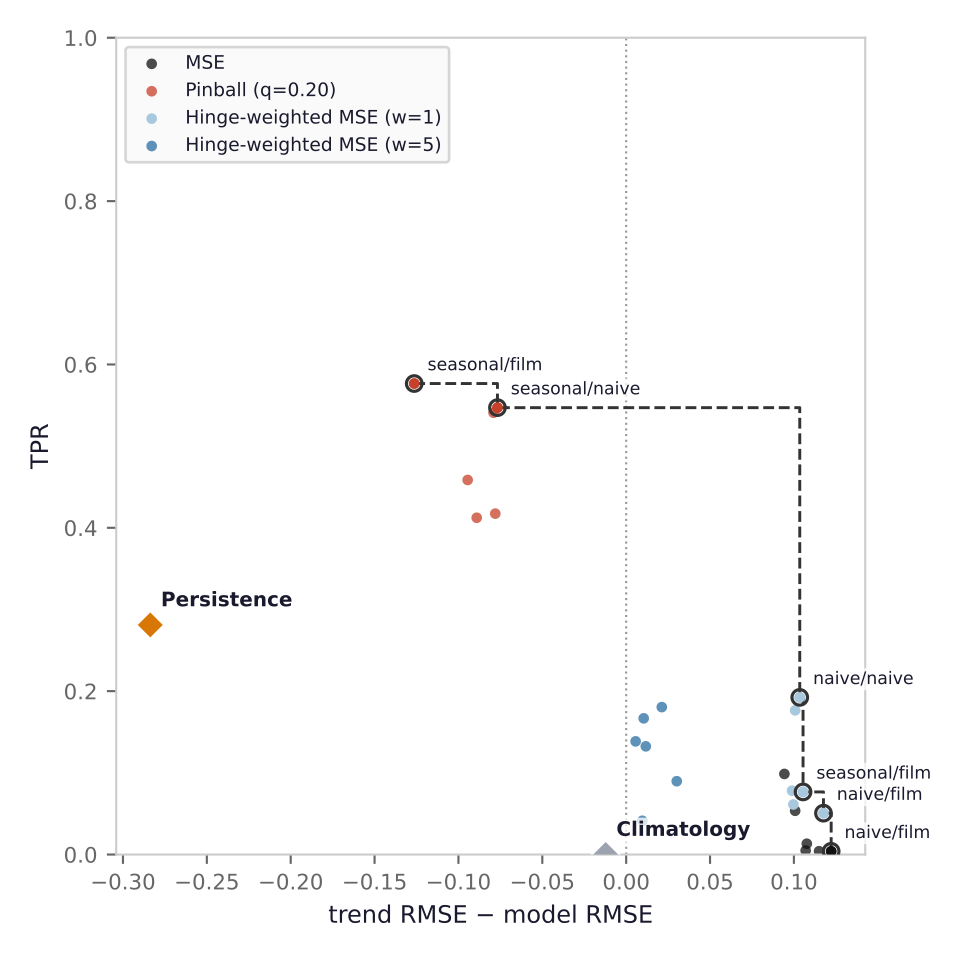
\includegraphics[width=0.48\linewidth]{work/02-drought_prediction/figures/frontier_tpr_light} 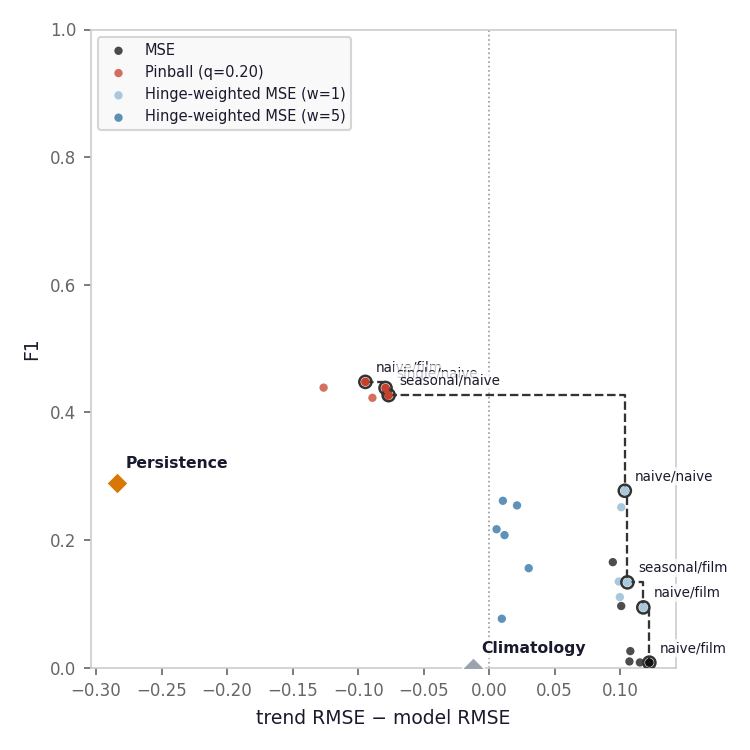
\includegraphics[width=0.48\linewidth]{work/02-drought_prediction/figures/frontier_f1_light} 

}

\caption{RMSE against drought detection, as TPR (left) and F1 (right), for all 24 configurations and the persistence and climatology baselines. The vertical line marks the linear-trend RMSE.}\label{fig:dp-frontier}
\end{figure}

\section{Discussion}\label{discussion-1}

A consistent picture emerges across the three comparisons.

\begin{itemize}
\tightlist
\item
  \textbf{RQ1:} The loss function governs the accuracy-detection trade-off more strongly than any other choice examined here: it moves a model from low RMSE and almost no detection (MSE) to high detection and high RMSE (Pinball).
\item
  \textbf{RQ2:} FiLM conditioning on the global dynamic variables helps only conditionally. It improves detection as compared to naive injection only under Pinball but costs detection under the other losses. In the drought tail it lowers error across the severe and extreme categories under every loss.
\item
  \textbf{RQ3:} Neither the learned single nor the seasonal topography encoder reliably improves on naive injection: both act mainly on detection in a similar loss-dependent way, and neither is consistently ahead.
\end{itemize}

Across the full grid of configurations the loss is the main lever, and no single setup dominates the Pareto front.

At a twelve-month lead in a complex region like the Alps, the task itself is hard.
Some of the models beat the simple linear-trend baseline on RMSE, but only by a small margin, and no configuration pulls far ahead.
The loss acts less as a way to extract more skill than as a way to choose an operating point on this trade-off, moving the model toward lower RMSE or toward higher detection.
Together, these factors could also explain why the feature-injection choices, which barely affect this basic tension, only move models short distances along the trade-off.

Because Pinball shifts predictions toward the dry tail, part of its detection edge could come from that shift, though it also wins on F1, which penalises false alarms, so it is not merely predicting more droughts blindly.
Nevertheless, its detection gains are best read together with the RMSE they cost.
The limited impact of the injection strategies may also be a reflection of the usefulness of the features themselves, since the achievable gains are bounded by how informative the injected features are.
Further analysis of feature importance is given in the appendix.

These conclusions should be seen in light of several limitations.
Each configuration was trained once, so the reported differences carry no estimate of run-to-run variance, and the smaller gaps should be read cautiously.
This work also only covers a single region, a single lead time, a single drought index (SPEI-1), and one fixed set of input features, so how far the loss-dominance and the feature-injection comparisons generalize is unclear.
The chronological split also leaves the test period drier than the training period, as severe-drought frequency rises across time, so the models are evaluated under a distribution shift rather than on identically distributed data.

\section{Conclusion}\label{conclusion-1}

This work compared loss functions and feature-injection strategies for a ConvLSTM forecasting SPEI-1 one year ahead over the Alps.
The main finding is that the loss is the dominant lever, fixing where the model sits on a trade-off between point accuracy and severe-drought detection, while the global and static feature injection strategies only change model performance marginally.
Future work should investigate whether these findings hold across multiple seeds or ensembles, more regions, shorter and more predictable forecasting horizons, and richer or differently chosen conditioning features.

\section*{Appendix: AI Declaration}\label{appendix-ai-declaration}


I hereby declare that this seminar thesis is my own work and that I have used no sources or aids other than those acknowledged.

During the preparation of this manuscript, generative AI tools were used in a supportive and transparent manner, in accordance with the guidelines of the Institute of Statistics at LMU Munich.
Specifically, Claude was used to assist with language formulation, stylistic refinement, and clarity of presentation across the whole manuscript.
All suggested formulations were critically reviewed and, where adopted, revised by me.

In addition, Claude and Claude Code were used selectively for programming support, including as a coding aid, for debugging assistance, and for minor refactoring suggestions.
All code was fully understood, tested, and validated by me, and I retain full responsibility for its correctness and functionality.

All scientific content, methodological decisions, analyses, and interpretations were developed by me, and I take full responsibility for the integrity and correctness of the work.

\section*{Appendix: SPEI drought classification}\label{appendix-spei-drought-classification}


SPEI values map onto standard drought categories (Table \ref{tab:dp-spei-grades}).
The severe and extreme categories, at the \(-1.5\) threshold and below, are the ones this work targets.

\begin{longtable}[]{@{}cll@{}}
\caption{\label{tab:dp-spei-grades} SPEI drought classification \citep{vicenteserrano2010, chen2025}.}\tabularnewline
\toprule\noalign{}
Grade & Category & SPEI range \\
\midrule\noalign{}
\endfirsthead
\toprule\noalign{}
Grade & Category & SPEI range \\
\midrule\noalign{}
\endhead
\bottomrule\noalign{}
\endlastfoot
1 & No drought & \(-0.5 < \text{SPEI}\) \\
2 & Light drought & \(-1.0 < \text{SPEI} \le -0.5\) \\
3 & Moderate drought & \(-1.5 < \text{SPEI} \le -1.0\) \\
4 & Severe drought & \(-2.0 < \text{SPEI} \le -1.5\) \\
5 & Extreme drought & \(\text{SPEI} \le -2.0\) \\
\end{longtable}

\section*{Appendix: Feature importance}\label{appendix-feature-importance}


Each input was occluded in turn (set to its training mean) and the frozen Pinball model re-scored on the test set \citep{zeiler2013}.
Inputs are occluded rather than permuted because the driver fields are correlated \citep{hooker2021}.

The left panel of Figure \ref{fig:dp-feat-importance} shows that point accuracy is unmovable, as every bar sits near zero and no input shifts the pooled RMSE by more than 0.06 in any configuration.
Detection (right panel) rests on a few inputs.
The Mediterranean SST is the strongest driver where no static encoder is present (the grey bars).
Adding a single or seasonal encoder raises the importance of near-surface temperature and lowers the SST's, though the two become comparable rather than temperature fully taking over.
FiLM changes this less than the static encoder does, though without an encoder it slightly deepens reliance on the global drivers it conditions on, lengthening the Mediterranean SST and month bars (the darker shade in each pair).
Topography is the one input whose removal raises TPR, and the remaining fields barely move it.

\begin{figure}

{\centering 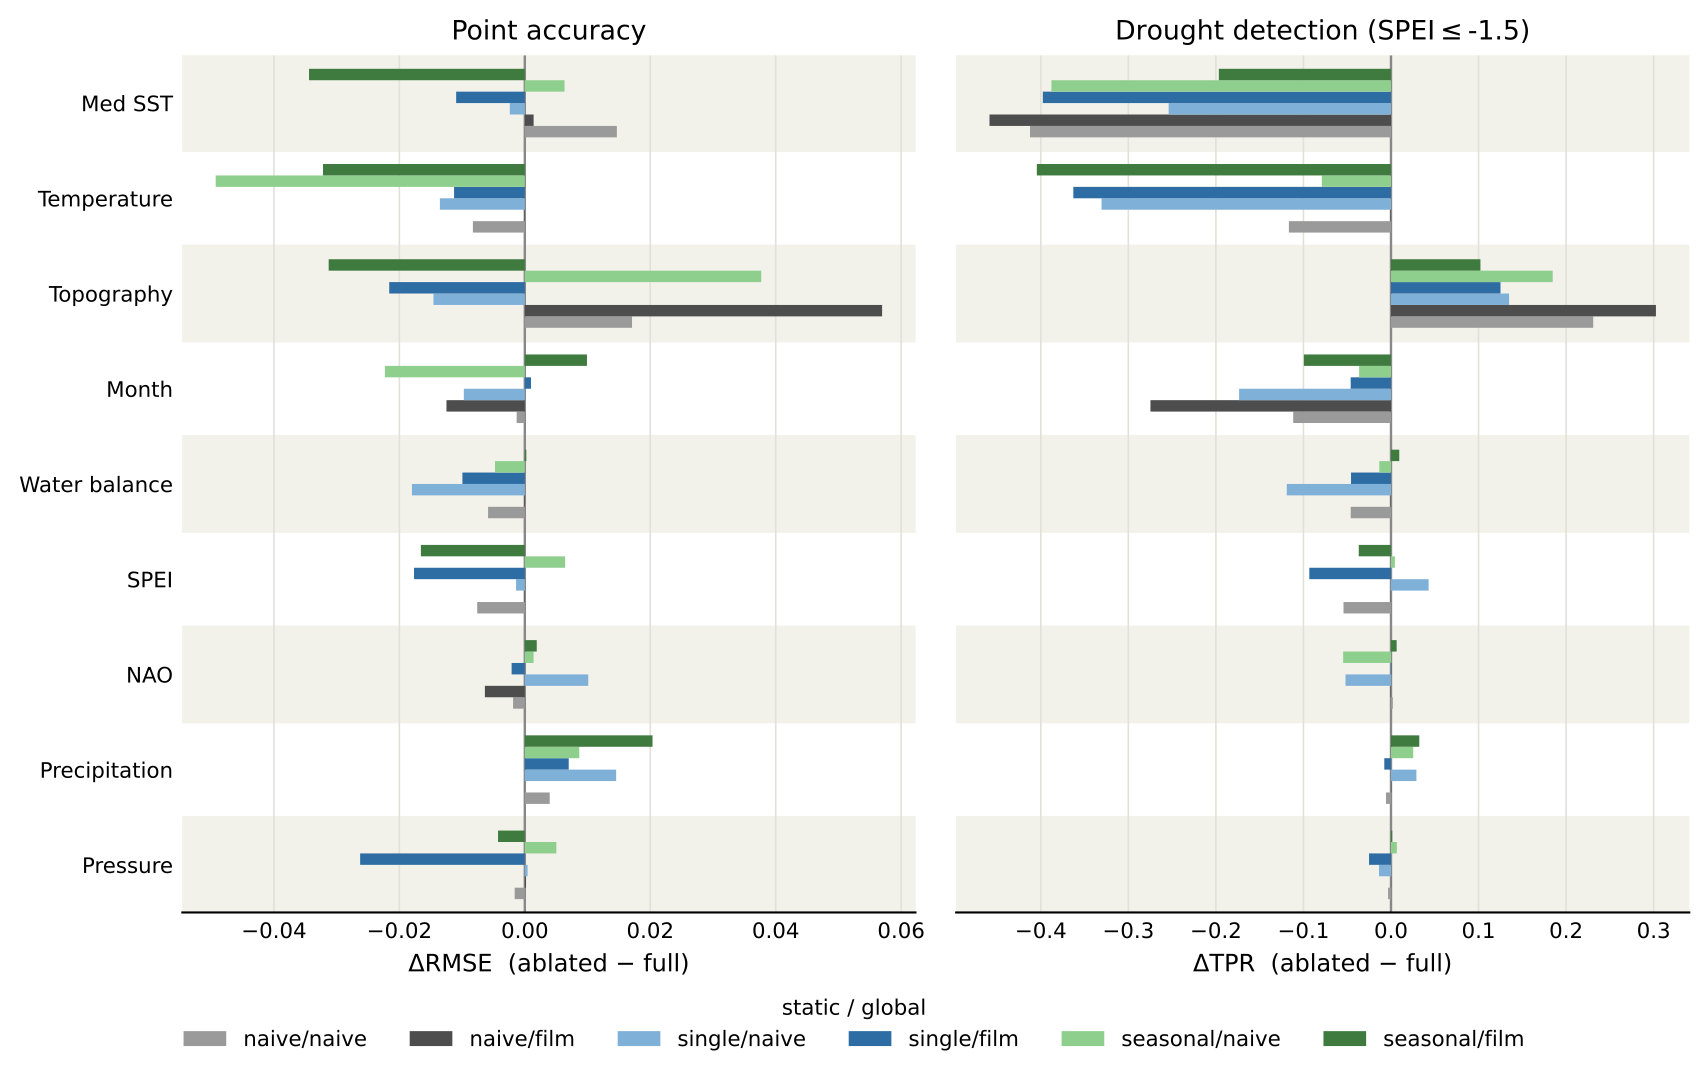
\includegraphics[width=0.95\linewidth]{work/02-drought_prediction/figures/interpretability/feature_importance_across_conditions} 

}

\caption{Occlusion feature importance for the Pinball models across all six architecture conditions. Change in pooled RMSE (left) and drought TPR (right) when each input is set to its training mean on the test set, configurations labelled static / global.}\label{fig:dp-feat-importance}
\end{figure}

\section*{Appendix: Implementation details}\label{appendix-implementation-details}


The two feature groups can either be appended to the input or routed through a learned pathway, which changes how many channels the ConvLSTM input \(x\) carries (Table \ref{tab:dp-input-channels}).

\begin{longtable}[]{@{}lcl@{}}
\caption{\label{tab:dp-input-channels} Input channels per configuration, from a dynamic base of five gridded variables. Naive injection appends features as channels, while the learned encoders (static CNN, FiLM) route them into a dedicated pathway.}\tabularnewline
\toprule\noalign{}
Static / global & \(x\) channels & Injected \\
\midrule\noalign{}
\endfirsthead
\toprule\noalign{}
Static / global & \(x\) channels & Injected \\
\midrule\noalign{}
\endhead
\bottomrule\noalign{}
\endlastfoot
naive / naive & 13 & +2 static, +6 global \\
single / naive & 11 & +6 global \\
seasonal / naive & 11 & +6 global \\
naive / FiLM & 7 & +2 static \\
single / FiLM & 5 & --- \\
seasonal / FiLM & 5 & --- \\
\end{longtable}

Beyond the protocol given in the main text, the initial embedding uses 16 channels and the ConvLSTM hidden state 32.
Early stopping monitors the validation RMSE median with patience 5 and a minimum delta of 0.003, and the learning rate follows ReduceLROnPlateau with patience 3.
The static encoder maps the two static channels to 16.

\chapter{Hydrology under Climate Change}\label{hyd}

\emph{Author: Rong Bao}

\emph{Supervisor: Henri Funk}

\emph{Degree: Bachelor}

\section{Abstract}\label{abstract-1}

Streamflow integrates the weather, geology and land cover of an entire catchment into a single measured quantity, which makes it a natural indicator of hydrological change. At the same time, rivers are noisy: they swing between wet and dry years on their own, and this natural variability can mask a slow climate-driven trend for decades. This chapter asks when, where, and in which seasons the climate-change signal in Swiss river flows becomes detectable above natural variability --- the \emph{time of emergence} (ToE) \citep{hawkins2012} --- and whether flow is increasing or decreasing. Using observed daily discharge from 209 quality-controlled catchments of the CAMELS-CH dataset (1981--2020) \citep{hoege2023}, the climate signal is separated from noise with a robust STL decomposition \citep{cleveland1990}, and emergence is declared when the signal-to-noise ratio (SNR) permanently exceeds a threshold of 1 (lenient) or 2 (strict). By 2020 only 19 of 209 rivers have emerged at the lenient threshold; extrapolating the robust Theil--Sen trend \citep{sen1968} suggests a median emergence year around 2046, while 73 rivers never emerge by 2100. Emergence is spatially structured: the low-elevation Jura and Plateau lead, while high Alpine regions are delayed in the annual analysis because winter increases and summer decreases partly cancel. A complementary per-season analysis shows that spring and summer are the sentinel seasons (about 70 \% of rivers emerged by 2100), and reveals a seasonal redistribution of water: winter flows predominantly rise while summer flows predominantly fall. Estimated emergence years carry substantial uncertainty and should be read as indicative; the direction, ordering and spatial-seasonal pattern of change are the robust results.

\section{Introduction}\label{introduction-2}

Hydrology is the study of water moving through the landscape: rain and snow fall, water is stored in soil, snowpack and glaciers, and eventually reaches the rivers. Streamflow --- the amount of water in a river --- is special among climate indicators because it aggregates the meteorological forcing and physical properties of a whole catchment into one number that is measured operationally, often for many decades.

One difficulty runs through any attempt to detect climate change in river flow: rivers are noisy. Even without any external forcing, discharge fluctuates strongly between wet and dry years and between decades. Natural variability in this sense is the year-to-year and decade-to-decade swing a river shows on its own; it has no long-term trend and averages to zero over time. A forced climate signal only becomes \emph{detectable} once it has grown large relative to this background --- the concept of the time of emergence, introduced for temperature by \citet{hawkins2012} and since applied across climate variables.

The way around the noisiness of individual records is scale: analysing not one river but hundreds at once. This is exactly what the recent \emph{large-sample hydrology} datasets enable. The research question of this chapter is therefore:

\begin{quote}
\textbf{When, where, and in which seasons does the climate-change signal in Swiss streamflow become detectable above natural variability --- and is the flow increasing or decreasing?}
\end{quote}

\section{Data}\label{data}

\subsection{The CAMELS family}\label{the-camels-family}

Large-sample hydrology requires data for hundreds of catchments in one consistent format. CAMELS (``Catchment Attributes and MEteorology for Large-sample Studies'') datasets package, for every gauged catchment in a region, three matched data types: (i) daily streamflow at the gauge, (ii) catchment-averaged meteorology (precipitation, temperature, potential evapotranspiration), and (iii) static attributes describing topography, climate, soil, geology and land cover \citep{addor2017}. Following the original US dataset, national versions exist for Great Britain \citep{coxon2020}, Brazil \citep{chagas2020}, Central Europe \citep{klingler2021} and North America \citep{arsenault2020}, among others, and the Caravan initiative merges them into a global community dataset \citep{kratzert2023}.

\subsection{CAMELS-CH and the case for Switzerland}\label{camels-ch-and-the-case-for-switzerland}

CAMELS-CH is the Swiss member of this family \citep{hoege2023}. It covers 331 catchments in hydrologic Switzerland over 40 years (1981--2020); about one third of the catchments extend into neighbouring countries. This chapter uses two components: the \textbf{observed} daily specific discharge (mm d\textsuperscript{-1}) --- simulated series are deliberately excluded, because the goal is to identify emergence directly from observations --- and the catchment boundary polygons, needed to assign every gauge to a reporting region.

Switzerland is a natural laboratory for this question. It is often called the ``water tower of Europe'', holding the largest share of the Alpine glacier mass, and change is already visible throughout its water cycle: Alpine snow cover has declined by more than 8 \% per decade since the early 1970s \citep{matiu2021}, glaciers have lost about half of their volume since 1931 \citep{mannerfelt2022}, flood frequency has increased in parts of the country since around 1970 \citep{schmockerfackel2010}, and the Alps are literally turning greener \citep{rumpf2022}. The broader water cycle is clearly changing; the precise question here is when that change becomes statistically visible in river discharge itself.

\subsection{Regions and preprocessing}\label{regions-and-preprocessing}

For reporting, catchments are grouped into the seven official FOEN bio-geographic regions (Fig. \ref{fig:hyd-regions}): Jura, the Black Forest border area, the Plateau, and the four Alpine regions Alps North, West, South and East. This grouping matters because Switzerland is not hydrologically uniform --- a low-elevation Plateau river and a high Alpine snowmelt river can respond very differently to warming. Regions are assigned by spatial overlay of the official region polygons with the CAMELS-CH catchment polygons; each catchment is assigned to the region covering the largest share of its area. About 20 \% of catchments cross a regional boundary.

\begin{figure}

{\centering 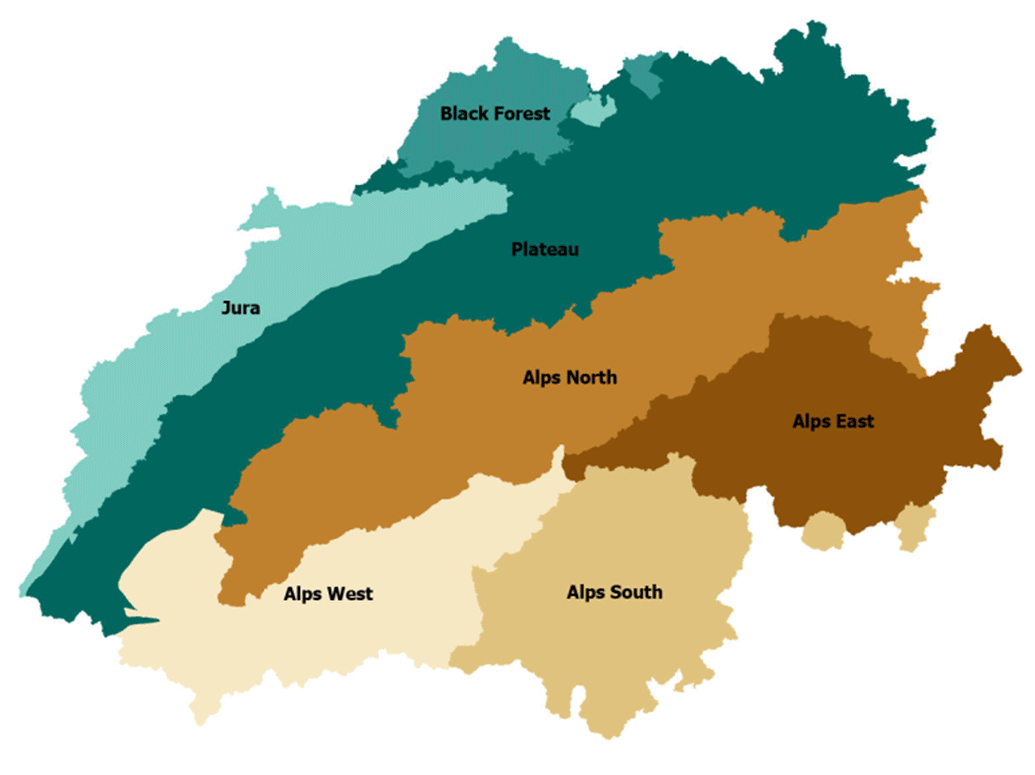
\includegraphics[width=0.85\linewidth]{work/03-hydrology_cc/figures/regions_of_swiss_map} 

}

\caption{The seven FOEN bio-geographic regions of Switzerland used for reporting. Adapted from @hoege2023 (Fig. 4); region polygons: Swiss Federal Office for the Environment (FOEN).}\label{fig:hyd-regions}
\end{figure}

Three preparation steps precede the analysis. First, daily discharge is aggregated to quarterly means using climatological seasons (DJF, MAM, JJA, SON; December is assigned to the following year's winter). Second, quality control: a quarter with more than 5 \% of daily values missing is dropped, and a station is excluded entirely if any of its seasonal series is more than 20 \% incomplete. After filtering, \textbf{209 of the 331 rivers} remain. Third, the regional assignment described above.

\section{Methods}\label{methods-2}

\subsection{Signal versus noise}\label{signal-versus-noise}

Any observed change in river flow can be decomposed into a forced, climate-related \textbf{signal} and \textbf{noise} --- natural variability including wet and dry years and extreme events that are not part of the long-term trend. A signal is detectable only when it is large compared with the noise, which motivates a signal-to-noise framework.

\subsection{STL decomposition}\label{stl-decomposition}

Alpine rivers have a strong seasonal cycle --- high flow in the melt season, low flow in winter --- which would dominate the analysis and inflate the noise if left in the series. STL (Seasonal-Trend decomposition using Loess) \citep{cleveland1990} writes the observed quarterly flow \(Y_t\) as three additive components,

\[
Y_t = T_t + S_t + R_t,
\]

where \(T_t\) is the slowly varying \textbf{trend} (used as the signal), \(S_t\) the regular within-year \textbf{seasonal cycle}, and \(R_t\) the \textbf{remainder} (used to estimate the noise).

STL assumes no parametric model; every component is built from one smoother, loess, applied inside two nested loops. Loess estimates the value at a target time \(x\) by taking the \(q\) nearest observations, scaling their distances by \(\lambda_q(x)\), the distance to the \(q\)-th nearest neighbour, down-weighting more distant points, and fitting a locally weighted regression. The \textbf{inner loop} alternates between updating the seasonal component --- smoothing each seasonal subseries (all winters together, all springs together, \ldots) and removing leftover trend with a low-pass filter --- and updating the trend by smoothing the deseasonalised series. The \textbf{outer loop} makes the procedure robust: points with extreme remainders receive small (or zero) robustness weights before the inner loop is repeated. This matters hydrologically because flood and drought years are real but should not bend the long-term trend; here the outer loop is iterated 15 times.

\subsection{Signal, noise, and time of emergence}\label{signal-noise-and-time-of-emergence}

The reference period is \textbf{1981--2000} (80 quarterly values), treated as the pre-change baseline. The signal at time \(t\) is the STL trend relative to its baseline mean, and the noise \(\sigma_N\) is the standard deviation of the STL remainder over the same period, so every river is scaled by its own baseline variability:

\[
\mathrm{SNR}(t) \;=\; \frac{T_t - \overline{T}_{\mathrm{ref}}}{\sigma_N},
\qquad
\sigma_N = \mathrm{sd}\!\left(R_t \,\middle|\, t \in \text{1981–2000}\right).
\]

The \textbf{time of emergence} is the first year in which \(|\mathrm{SNR}(t)|\) crosses a threshold and stays beyond it until the end of the record. Two thresholds are reported, following the time-of-emergence literature \citep{hawkins2012}: a lenient level \(|\mathrm{SNR}| \ge 1\) and a strict level \(|\mathrm{SNR}| \ge 2\).

To extend the analysis beyond 2020, the trend is extrapolated with the \textbf{Theil--Sen slope} \citep{sen1968}: the median of the slopes between all pairs of time points (12,720 pairwise slopes for 160 quarters). The median is stable because a single extreme event can affect some pairs but cannot easily control the middle of the distribution.

\subsection{A worked example}\label{a-worked-example}

Figures \ref{fig:hyd-stl-overlay} and \ref{fig:hyd-stl-snr} illustrate the pipeline for gauge 2219. The observed quarterly series (grey) is strongly seasonal and noisy; STL separates the seasonal cycle (pink: trend + seasonality) from the smooth trend (blue). For this river the baseline trend mean is 5.40 mm d\textsuperscript{-1} and the baseline noise is 0.89 mm d\textsuperscript{-1}. The Theil--Sen slope is positive, about +0.22 mm d\textsuperscript{-1} per decade, so this river is getting wetter in the trend component. By 2020 the SNR reaches 0.67 --- below the lenient threshold, so the signal has not yet emerged within the observed record; extrapolation puts lenient emergence at 2034 and strict emergence at 2073.

\begin{figure}

{\centering 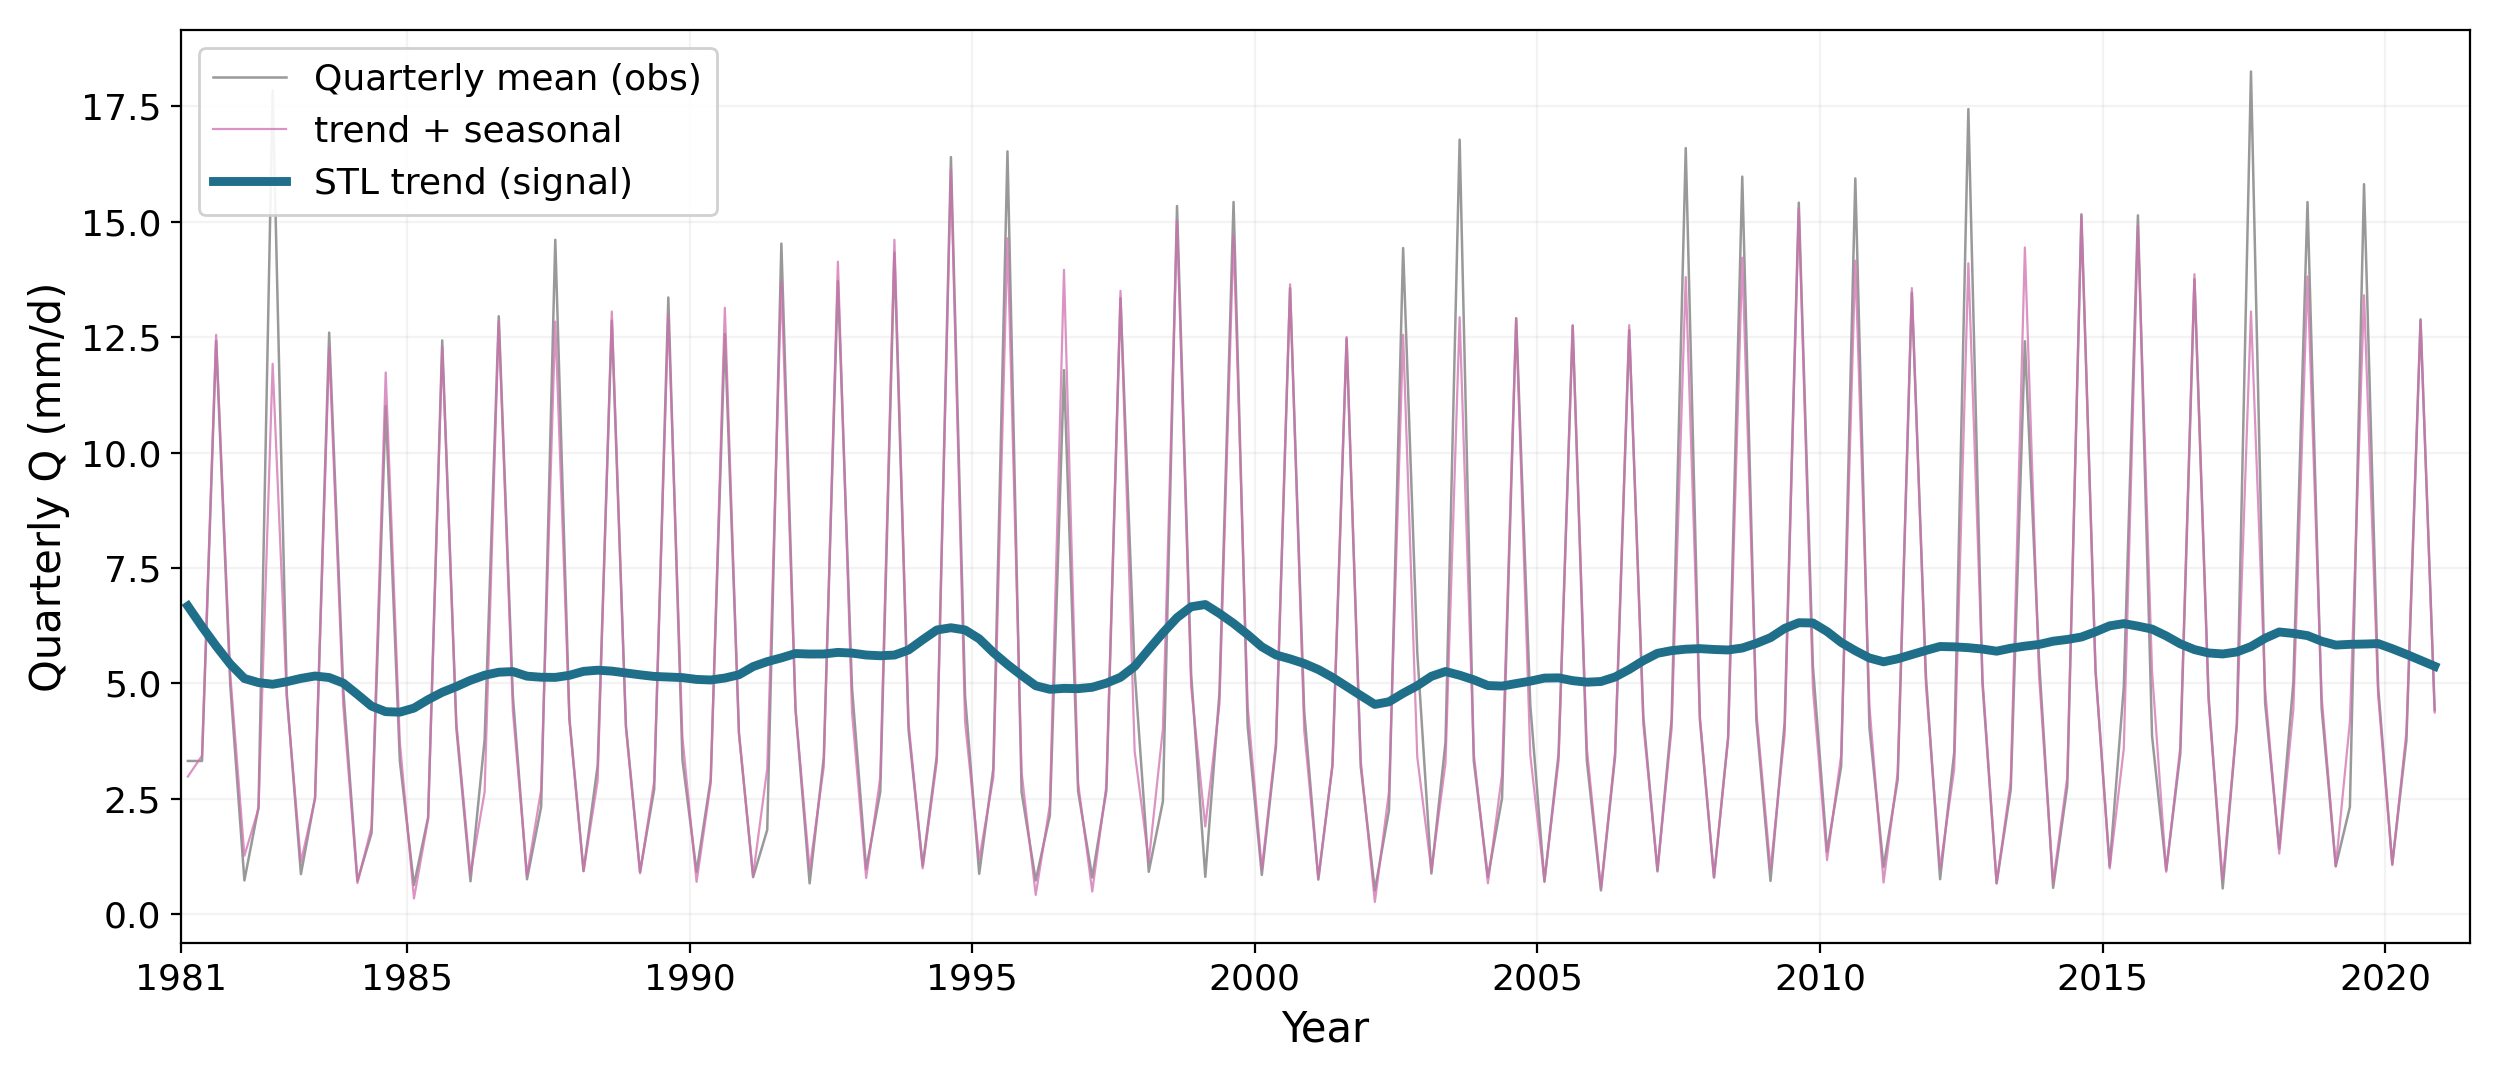
\includegraphics[width=0.9\linewidth]{work/03-hydrology_cc/figures/stl_example_overlay} 

}

\caption{Worked example (gauge 2219): observed quarterly flow (grey), STL trend plus seasonality (pink) and STL trend (blue).}\label{fig:hyd-stl-overlay}
\end{figure}

\begin{figure}

{\centering 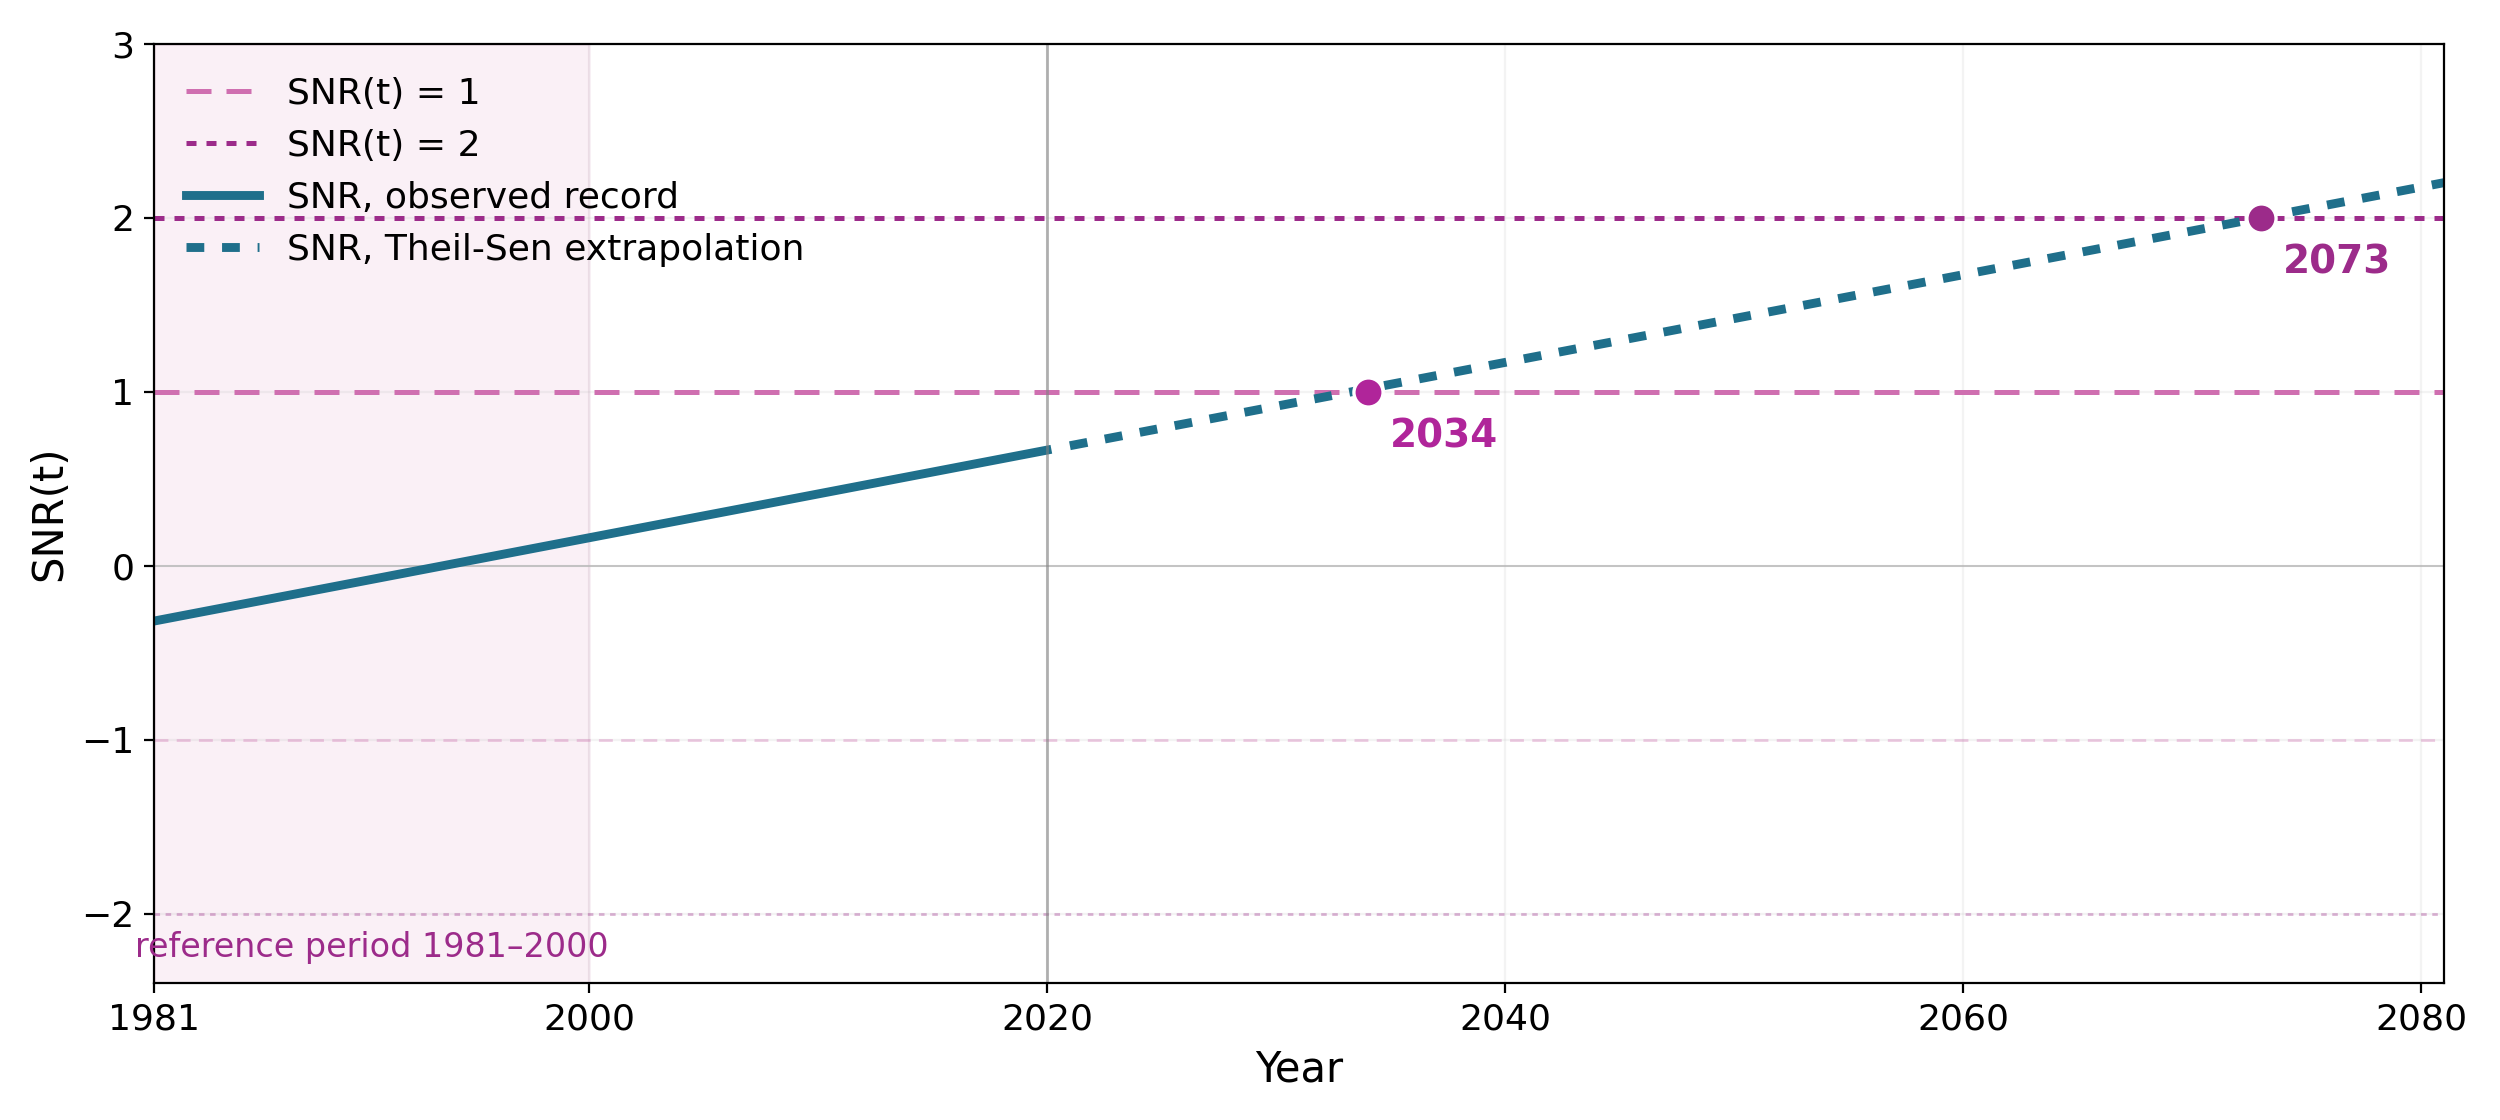
\includegraphics[width=0.9\linewidth]{work/03-hydrology_cc/figures/stl_example_snr} 

}

\caption{Worked example (gauge 2219): the trend standardised by baseline noise, with the lenient and strict emergence thresholds and the extrapolated Theil–Sen trend.}\label{fig:hyd-stl-snr}
\end{figure}

\section{Results}\label{results-2}

\subsection{Annual emergence and threshold sensitivity}\label{annual-emergence-and-threshold-sensitivity}

Across all 209 analysable rivers, the choice of threshold matters greatly for the numbers but not for the conclusion (Table \ref{tab:hyd-thresholds}). At the lenient threshold, 19 rivers have already emerged by 2020, another 117 are projected to emerge by 2100 (median emergence year around 2046), and 73 never emerge by 2100. At the strict threshold only 2 rivers have emerged, 71 are projected to emerge, and 136 never do. Either way, most annual-flow emergence is not yet visible in 2020 --- it happens after mid-century.

\begin{table}

\caption{\label{tab:hyd-thresholds}Threshold sensitivity of annual emergence (209 rivers).}
\centering
\begin{tabular}[t]{lrrr}
\toprule
Threshold & Emerged by 2020 & Projected 2021--2100 & Never by 2100\\
\midrule
Lenient ($\lvert\mathrm{SNR}\rvert \ge 1$) & 19 & 117 & 73\\
Strict ($\lvert\mathrm{SNR}\rvert \ge 2$) & 2 & 71 & 136\\
\bottomrule
\end{tabular}
\end{table}

How certain are these years? Of the 136 rivers that emerge at the lenient threshold, only 19 do so within the observed record; all other years are extrapolations. Each estimated year therefore carries an error bar --- formally about ±5 years, realistically 10--20 years, widening into the future (Fig. \ref{fig:hyd-uncertainty}). The direction and the \emph{ordering} of emergence are trustworthy; any single year should be read as ±a decade, and anything past 2080 as indicative only.

\begin{figure}

{\centering 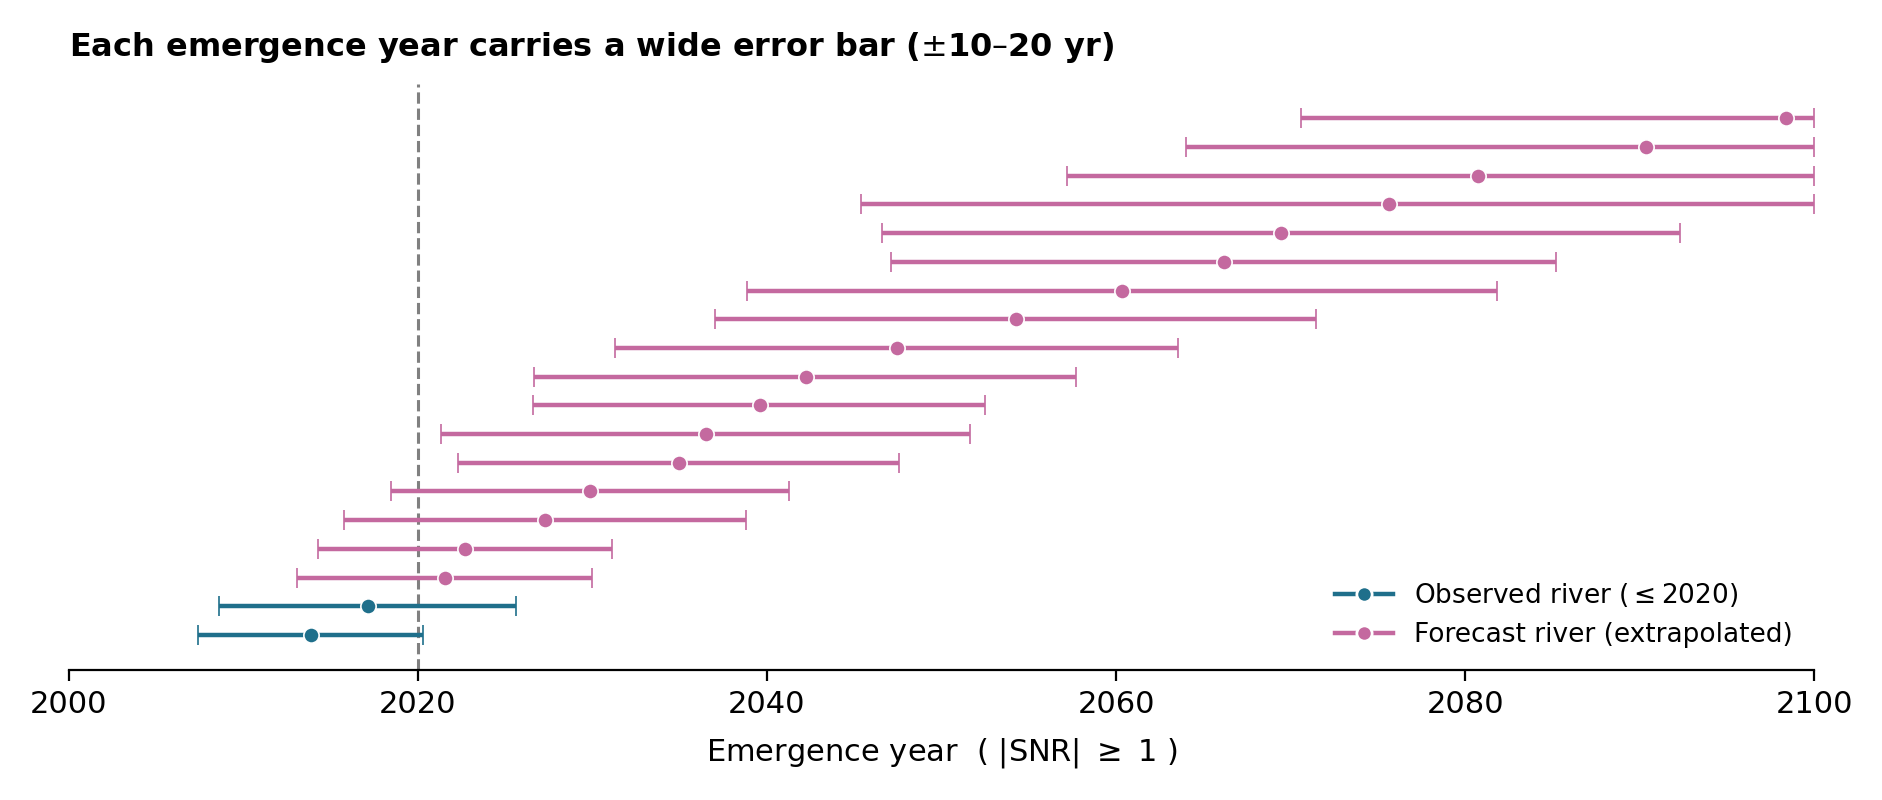
\includegraphics[width=0.9\linewidth]{work/03-hydrology_cc/figures/emergence_year_uncertainty} 

}

\caption{Uncertainty of estimated emergence years: the dark band shows the formal range (about $\pm$5 years), the pale band a realistic range (10--20 years), widening into the future.}\label{fig:hyd-uncertainty}
\end{figure}

\subsection{Regional patterns: low elevations lead}\label{regional-patterns-low-elevations-lead}

Emergence is spatially structured (Fig. \ref{fig:hyd-extent-region}). The low-to-mid elevation regions climb fastest: by 2050 the Jura reaches 78 \% emerged and the Plateau 62 \%. The high Alpine regions are slower --- Alps North, East and South reach only about 40--60 \% by 2100, with Alps South slowest at roughly 40 \%. This may seem surprising given how strongly the Alps are affected by warming, but in high Alpine catchments winter \emph{increases} and summer \emph{decreases} can partly cancel in the annual mean, delaying annual emergence --- a first hint that the annual perspective hides the real fingerprint.

\begin{figure}

{\centering 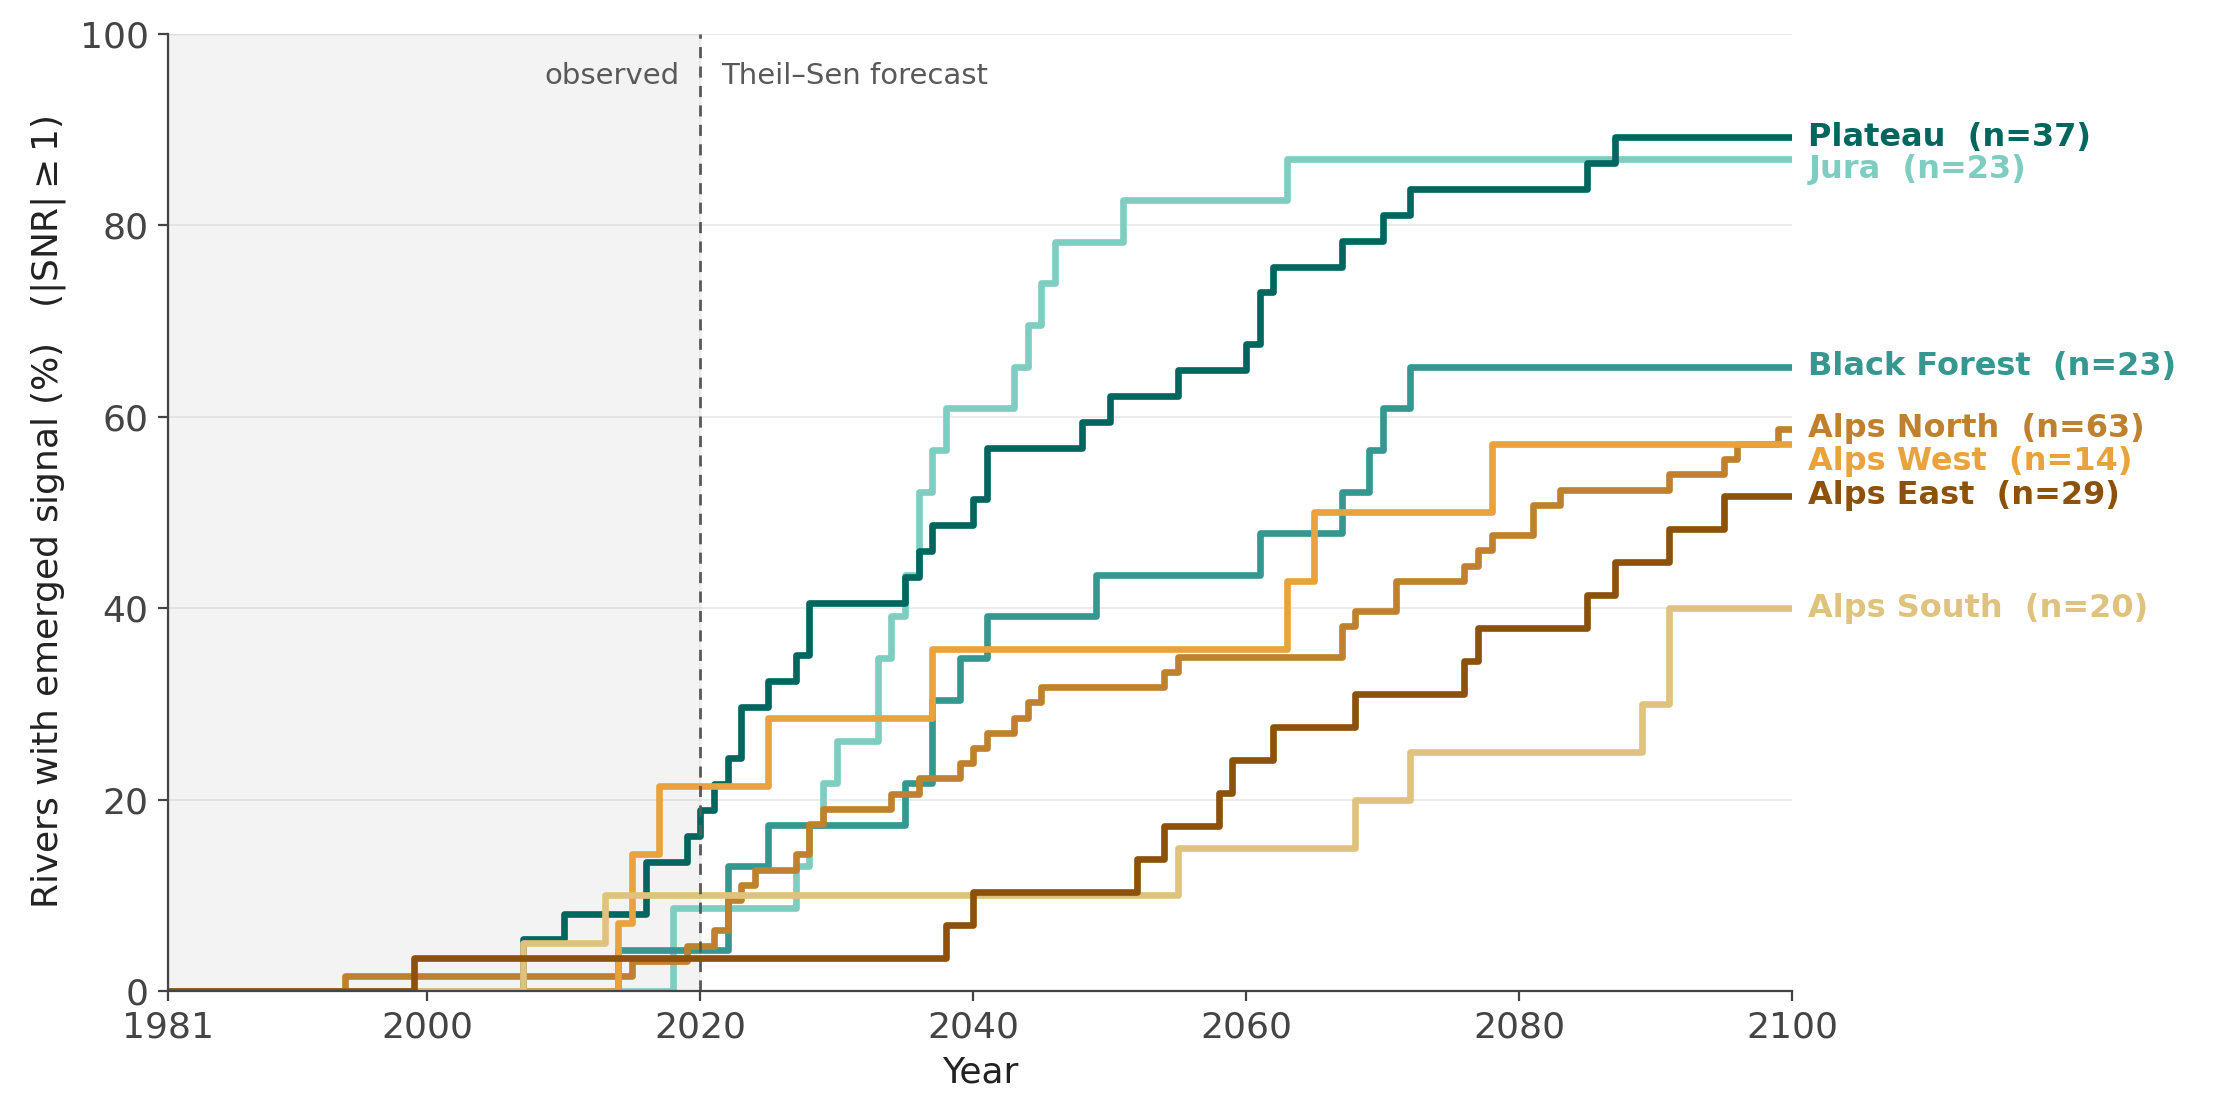
\includegraphics[width=0.95\linewidth]{work/03-hydrology_cc/figures/emergence_extent_by_region} 

}

\caption{Cumulative share of rivers with an emerged annual signal over time, by bio-geographic region (lenient threshold).}\label{fig:hyd-extent-region}
\end{figure}

\subsection{Seasonal analysis: spring and summer as sentinels}\label{seasonal-analysis-spring-and-summer-as-sentinels}

Climate change in Alpine hydrology has a seasonal fingerprint: snow storage, snowmelt timing, glacier melt and rainfall affect different seasons differently. For each gauge, four annual series are built (one value per year for DJF, MAM, JJA, SON). Since each series has one value per year, no within-year cycle remains and STL is not re-applied; instead the signal is a Theil--Sen robust line, the noise is the standard deviation of detrended residuals over 1981--2000, and the emergence rule is unchanged.

By 2020 the emerged share is still around 10 \% in every season; the seasons then separate (Fig. \ref{fig:hyd-seasonal-curves}). By 2050 spring, summer and autumn reach about 40--44 \% while winter lags at 31 \%; by 2100 spring reaches 71 \% and summer 70 \%, against 59 \% in autumn and 53 \% in winter. \textbf{Spring and summer are the sentinel seasons} --- not the only seasons changing, but those where emergence becomes most widespread.

\begin{figure}

{\centering 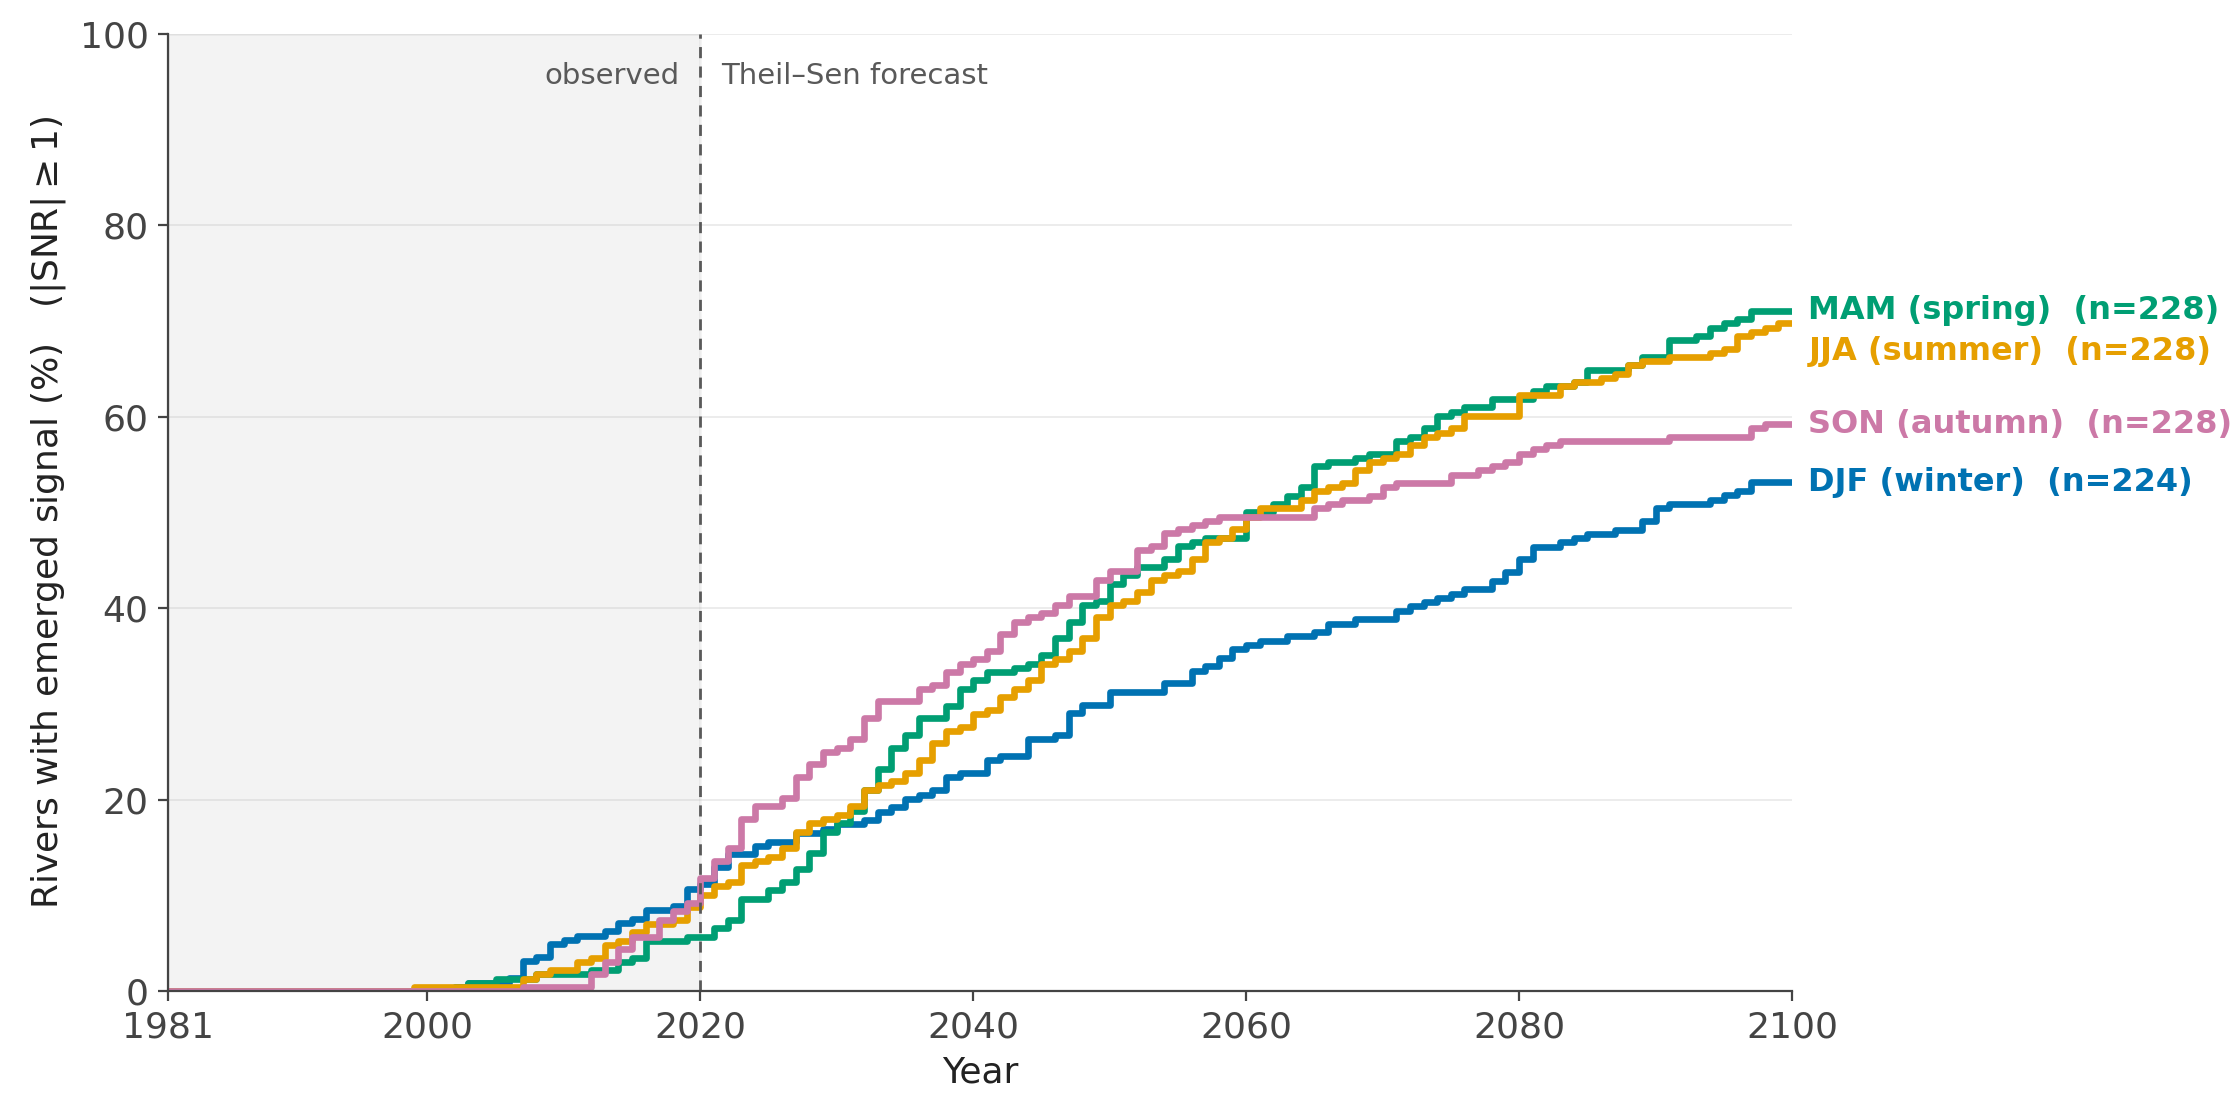
\includegraphics[width=0.95\linewidth]{work/03-hydrology_cc/figures/seasonal_emergence_extent_curves} 

}

\caption{Emerged share of rivers over time for each season (lenient threshold).}\label{fig:hyd-seasonal-curves}
\end{figure}

\subsection{Direction of change: winter up, summer down}\label{direction-of-change-winter-up-summer-down}

The directional split is clean (Fig. \ref{fig:hyd-direction-bars}). Winter is the only season where rises dominate: 39 \% of winter rivers show a rising signal by 2100 against 14 \% falling. Every other season is dominated by declines, most extremely summer, where 64 \% of rivers decline and only 6 \% rise. A plausible mechanism is the classic Alpine fingerprint: warming turns winter snowfall into rain and shifts snowmelt earlier, so more water leaves in winter and less meltwater remains for summer. The data thus show a \emph{seasonal redistribution} of water --- more flow in winter, less in the rest of the year --- which is partly hidden in annual averages.

\begin{figure}

{\centering 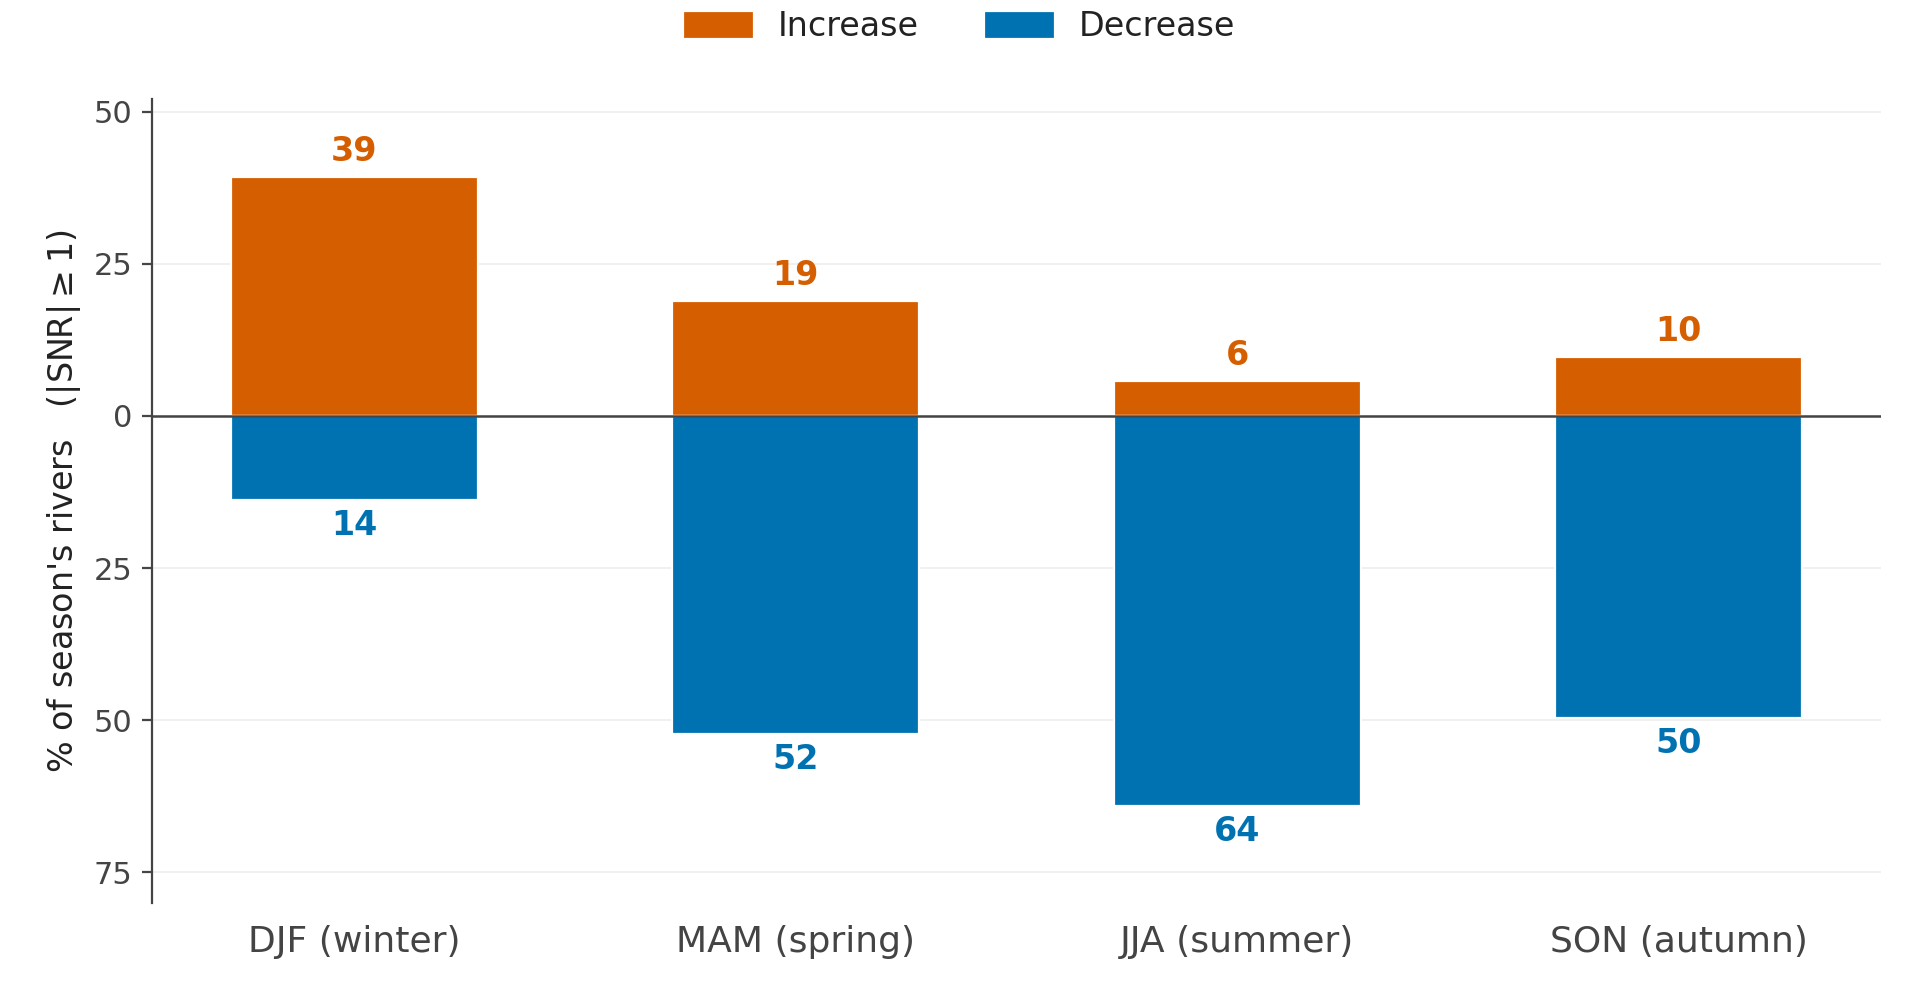
\includegraphics[width=0.9\linewidth]{work/03-hydrology_cc/figures/seasonal_direction_bars} 

}

\caption{Share of rivers per season whose signal emerges by 2100 with rising versus falling direction (lenient threshold); the gap to 100\% corresponds to rivers that never emerge.}\label{fig:hyd-direction-bars}
\end{figure}

The direction also varies systematically by region (Fig. \ref{fig:hyd-direction-region}). Winter increases are concentrated in the high Alps (86 \% of emerged rivers rising in Alps South, 80 \% in Alps East), while low regions are mixed. In summer, declines dominate everywhere (83 \% in Alps East, 76 \% in Alps West, 71 \% in Alps North, 60 \% on the Plateau). Spring shows the sharpest contrast: strongly decreasing in the low regions (Jura 96 \%, Plateau 76 \%, Black Forest 71 \%) while the western, southern and eastern Alps retain 43--47 \% increasing shares. In autumn, decreases dominate almost everywhere (Jura 100 \%, Alps West 88 \%, Plateau 67 \%). The winter-up signal is an Alpine signal; the decreases appear first and most completely in the low regions.

\begin{figure}

{\centering 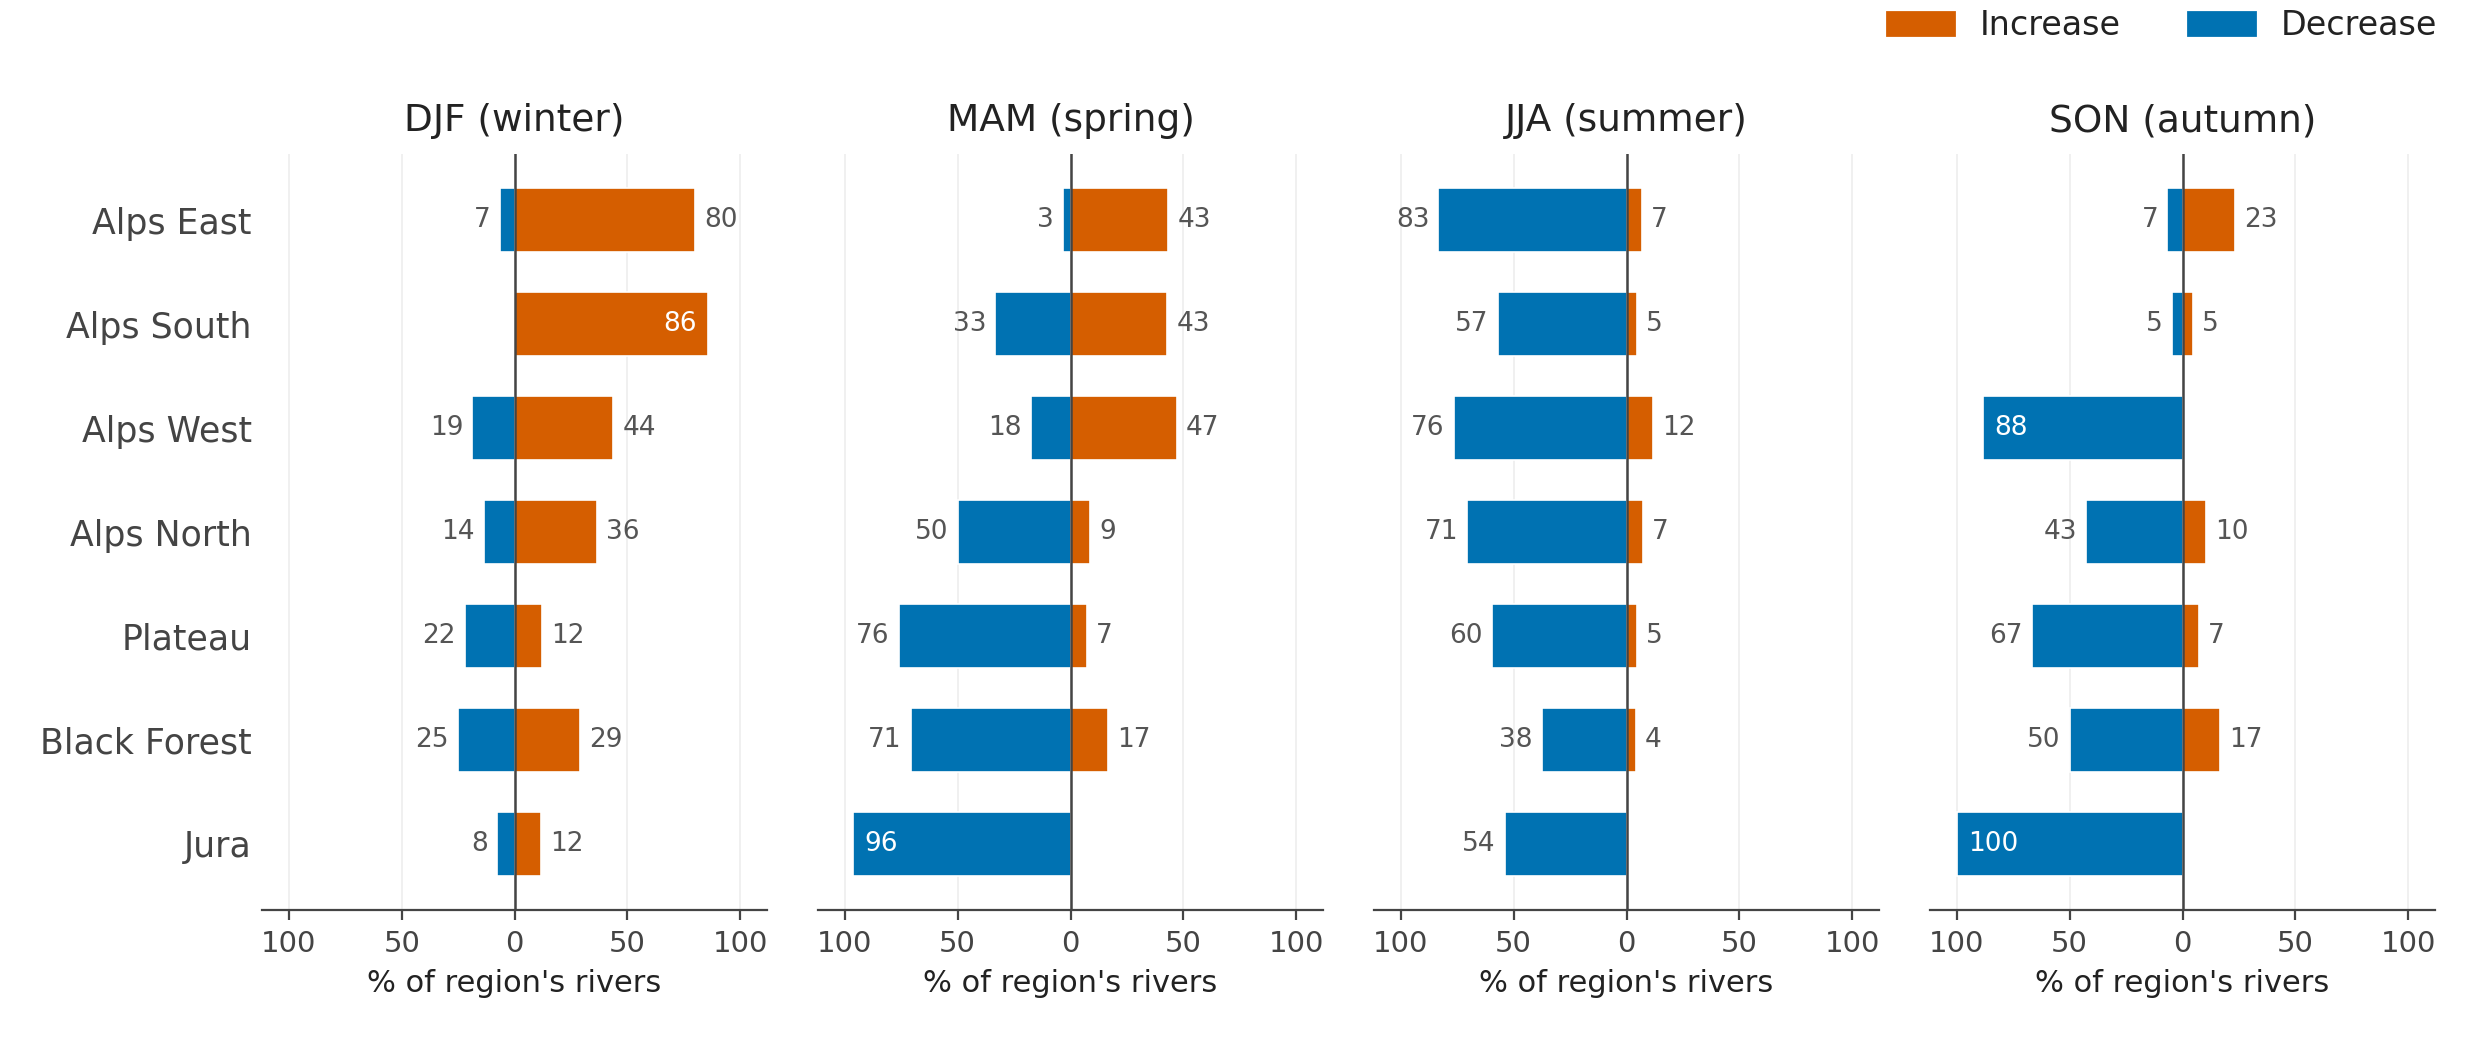
\includegraphics[width=0.95\linewidth]{work/03-hydrology_cc/figures/seasonal_direction_by_region} 

}

\caption{Direction of the emerged signal by 2100, split by season and bio-geographic region: share of emerged rivers with rising (red) versus falling (blue) flow.}\label{fig:hyd-direction-region}
\end{figure}

Finally, the season-by-region heatmap (Fig. \ref{fig:hyd-heatmap}) gives the fine structure of emergence extent by 2100. In winter, emergence climbs with elevation, from 19 \% in the Jura to 86--87 \% in Alps South and East. Spring is almost the mirror image, strongest in the low regions (Jura 96 \%, Black Forest 88 \%, Plateau 83 \%) and weakest in Alps East (47 \%). Summer peaks in the Alps (Alps East 90 \%, Alps West 88 \%, Alps North 78 \%), and autumn is the most uneven row (Jura 100 \%, Alps West 88 \%, but Alps South only 10 \%). Every region has at least one season with high emergence --- but \emph{which} season differs systematically.

\begin{figure}

{\centering 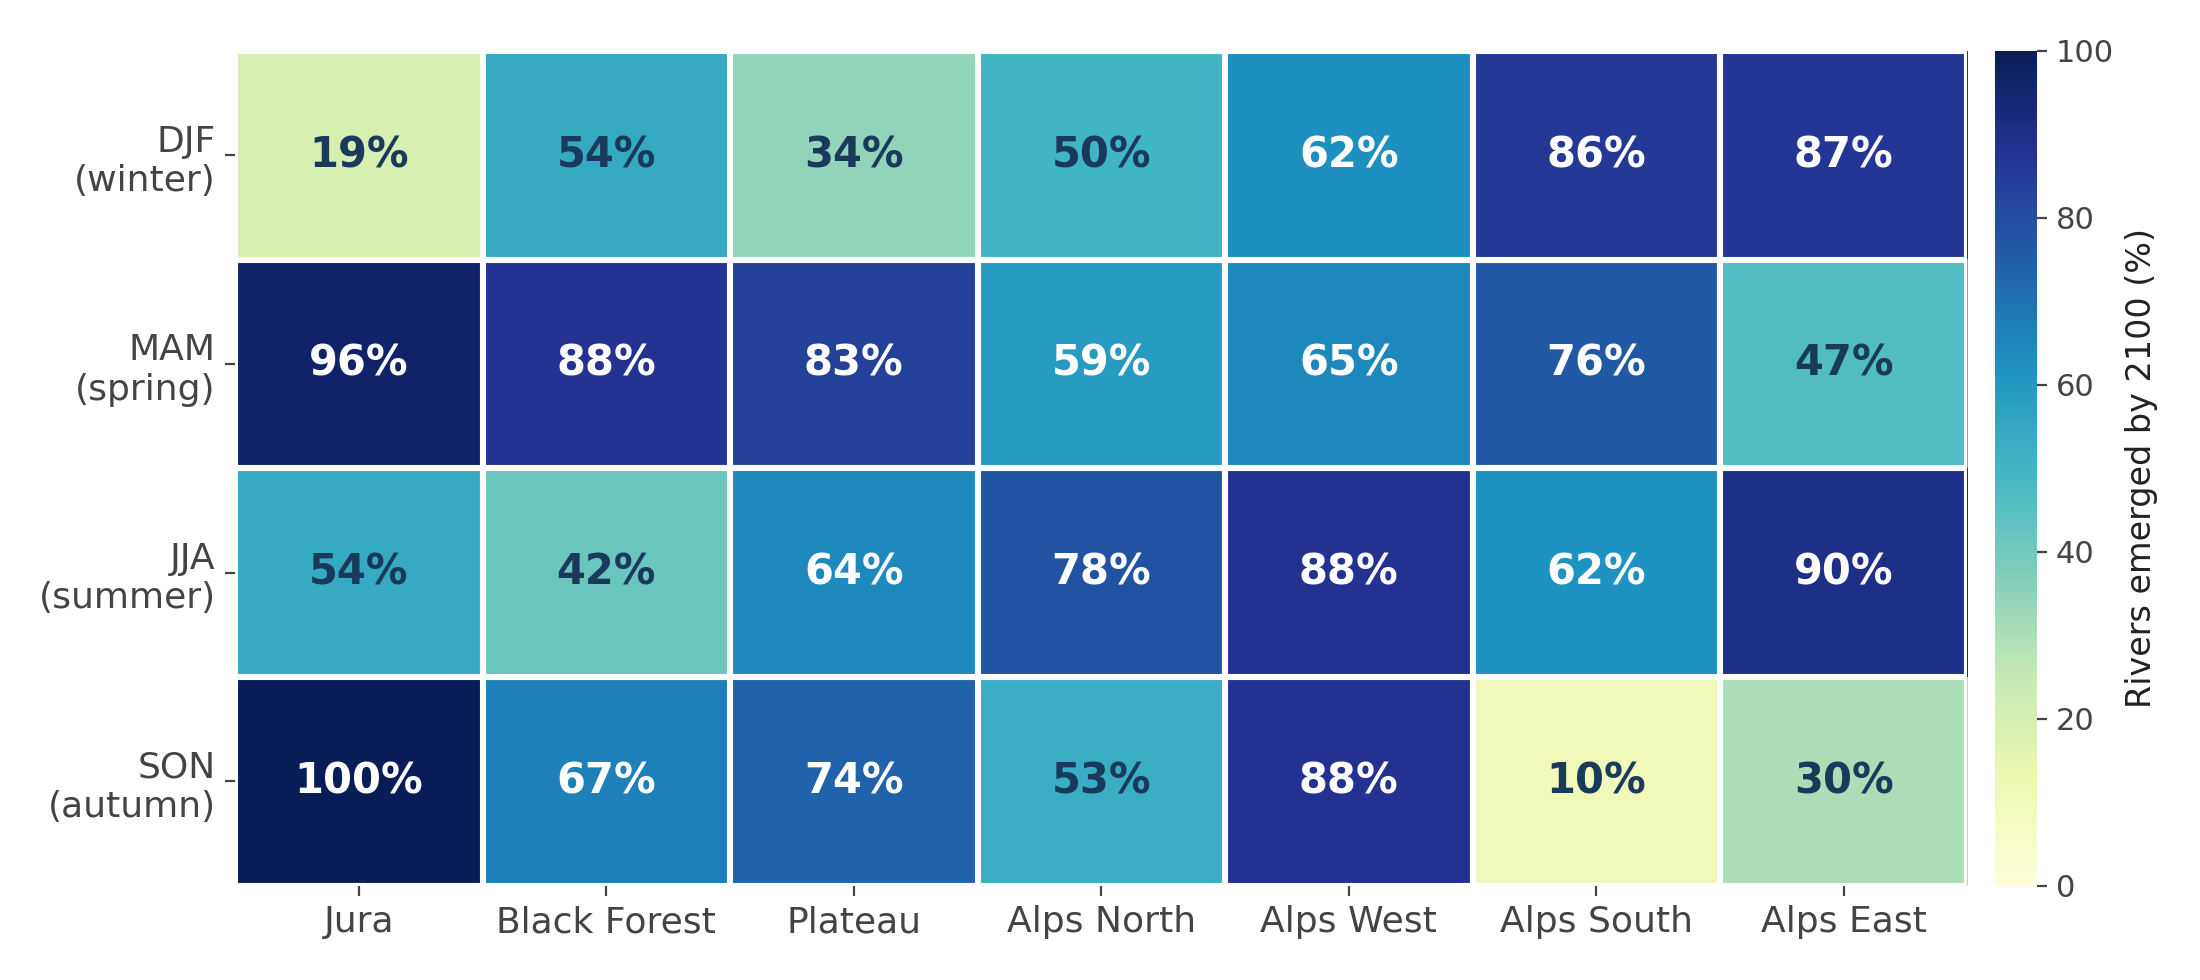
\includegraphics[width=0.95\linewidth]{work/03-hydrology_cc/figures/seasonal_emergence_heatmap} 

}

\caption{Season-by-region heatmap: share of rivers whose signal emerges by 2100 at the lenient threshold, in either direction.}\label{fig:hyd-heatmap}
\end{figure}

\section{Conclusion}\label{conclusion-2}

Five points summarise this chapter. \textbf{Method}: the signal is the STL trend relative to the 1981--2000 baseline, scaled by baseline noise; emergence is the first lasting crossing of an SNR threshold. \textbf{Timing}: of 209 rivers, only 19 have emerged by 2020 at the lenient threshold; the median projected emergence year is around 2046, and 73 rivers never emerge by 2100. \textbf{Geography}: the Jura and Plateau lead (62--78 \% emerged by 2050), while the high Alpine regions are slower in the annual analysis. \textbf{Season}: spring and summer are the sentinel seasons, each reaching about 70 \% of rivers emerged by 2100. \textbf{Direction}: winter up, summer down --- winter is the only season where rises dominate (39 \% of rivers), while summer declines most (64 \% falling).

The strength of this analysis lies in the direction, the spatial and seasonal pattern, and the \emph{relative} timing of change --- which regions and seasons emerge earlier than others. The specific emergence years are estimates with substantial error bars; their value is comparative, not predictive. A useful monitoring strategy for Swiss rivers should therefore be seasonal and regional, not only national and annual.

\chapter{Neural Hydrology}\label{nh-neural-hydrology}

\emph{Author: Yuxin Qiu}\\
\emph{Supervisor: Henri Funk}\\
\emph{Degree: Bachelor}

\section{Abstract}\label{nh-abstract}

Hydrological prediction under climate variability is a central challenge in environmental
statistics, especially when regional observations are limited and hydro-climatic
conditions deviate from historical norms. This chapter presents a detailed investigation
of neural hydrology, with emphasis on recurrent deep learning architectures and transfer
learning strategies for streamflow forecasting. We first position neural methods in
relation to classical process-based models, then formalize sequence-learning principles
that allow Long Short-Term Memory (LSTM) networks to represent delayed catchment memory
effects. We further examine physically informed variants, including mass-conserving
architectures, as mechanisms to improve structural plausibility under distributional
shift.

The empirical component uses CAMELS-US data and a three-way comparison framework across
local-from-scratch training, global pretraining, and global-to-local fine-tuning over
18 geographic groups. Results are analyzed with basin-weighted NSE and KGE, group-level
contrasts, basin-level distributional diagnostics, and architecture cross-checks. Across
evaluation views, fine-tuning provides consistent gains over local-only baselines and
additional improvement over zero-shot global inference in this benchmark setting.
Interpretation is framed through bias-variance trade-offs, representation reuse, and
regional adaptation dynamics.

Overall, the chapter argues that neural hydrology should be understood not merely as a
high-performance forecasting tool, but as a statistical modeling framework where
data-driven representation learning, physical constraints, and transfer protocols can be
jointly optimized for robust prediction under non-stationary climate conditions.

\section{Introduction}\label{nh-introduction}

Streamflow prediction, that is, estimating river discharge from meteorological forcings,
is one of the oldest and most consequential tasks in hydrology. Accurate forecasts are
critical for flood early-warning systems, reservoir operation, drought monitoring, and
hydropower planning. Under climate change, this task becomes harder because forcing
regimes are increasingly non-stationary: precipitation intensity distributions,
temperature seasonality, and snowmelt timing all shift over time \citep{ipcc2021carbon}.

This chapter reviews the emergence of deep learning as the leading paradigm for
data-driven streamflow modelling, introduces the \textbf{NeuralHydrology} Python library,
discusses architectures that embed physical constraints into neural networks, and
explores strategies for transfer learning in a non-stationary climate.

From a statistical perspective, the central object is a conditional forecasting function
\(f_\theta\) that maps a multivariate hydro-meteorological history and static basin
descriptors to a discharge distribution:

\[
\hat{q}_{t+\tau} \sim f_\theta\Big(\mathbf{x}_{1:t}, \mathbf{z}, \tau\Big),
\]

where \(\mathbf{x}_{1:t}\) denotes dynamic forcings up to time \(t\), \(\mathbf{z}\) denotes
time-invariant basin attributes, and \(\tau\) is the lead-time index. In deterministic
setups, one models the conditional mean \(\mathbb{E}[q_{t+\tau}\mid\mathbf{x}_{1:t},\mathbf{z}]\);
in probabilistic setups, one models the full predictive density
\(p(q_{t+\tau}\mid\mathbf{x}_{1:t},\mathbf{z})\).

The hydrological difficulty is that this map is high-dimensional, nonlinear, delayed,
and non-stationary. Hence, the chapter emphasizes three scientific questions:

\begin{enumerate}
\def\labelenumi{\arabic{enumi}.}
\tightlist
\item
  How can sequence models approximate memory-dependent rainfall-runoff dynamics?
\item
  How can physical constraints improve plausibility under extrapolation?
\item
  How can transfer learning reduce estimation variance in data-scarce regions?
\end{enumerate}

\begin{center}\rule{0.5\linewidth}{0.5pt}\end{center}

\section{Background: From Process-Based to Data-Driven Models}\label{nh-background}

\subsection{Traditional Process-Based Models}\label{traditional-process-based-models}

Classical hydrological models describe catchment behaviour through systems of differential
equations representing physical processes: precipitation infiltration, evapotranspiration,
soil moisture routing, and channel flow. Well-known examples include:

\begin{itemize}
\tightlist
\item
  \textbf{HBV} (Hydrologiska Byrans Vattenbalansavdelning) - a bucket-type conceptual model
\item
  \textbf{VIC} (Variable Infiltration Capacity) - a distributed land-surface model
\item
  \textbf{SAC-SMA} (Sacramento Soil Moisture Accounting) - used operationally by NOAA
\end{itemize}

These models are physically interpretable and operate well in data-sparse settings.
However, they suffer from three fundamental limitations:

\begin{enumerate}
\def\labelenumi{\arabic{enumi}.}
\tightlist
\item
  \textbf{Parameter estimation} - many parameters (soil depth, hydraulic conductivity,
  recession coefficients) cannot be measured directly and must be calibrated
  separately for each catchment.
\item
  \textbf{Spatial heterogeneity} - parameter sets calibrated for one catchment cannot be
  directly transferred to ungauged basins.
\item
  \textbf{Non-stationarity} - parameters calibrated under historical climate conditions may
  not hold under future climate forcing \citep{milly2008}.
\end{enumerate}

\subsection{Process-Based Formulation and Structural Error}\label{process-based-formulation-and-structural-error}

For a conceptual catchment model, storage dynamics can be represented generically as:

\[
S_{t+1} = S_t + P_t - ET_t - Q_t - L_t,
\]

where \(S_t\) is catchment storage, \(P_t\) precipitation input, \(ET_t\) evapotranspiration,
\(Q_t\) discharge, and \(L_t\) unobserved losses (deep percolation, abstraction, or closure
error). Practical model implementations replace these terms with parameterized
constitutive relationships, for example:

\[
Q_t = g_\phi(S_t, \mathbf{u}_t), \quad ET_t = h_\psi(S_t, T_t, R_t, V_t),
\]

with calibration parameters \((\phi,\psi)\) and meteorological covariates \(\mathbf{u}_t\).
Calibration thus solves an inverse problem that is often ill-posed: multiple parameter
sets can yield similar hydrographs (equifinality), while parameter meaning can vary with
the chosen process simplifications.

This generates two conceptually different errors:

\begin{enumerate}
\def\labelenumi{\arabic{enumi}.}
\tightlist
\item
  \textbf{Parametric uncertainty}: insufficient data to identify parameters uniquely.
\item
  \textbf{Structural uncertainty}: omitted or misspecified process mechanisms.
\end{enumerate}

Deep learning approaches primarily target structural flexibility by reducing the need to
prescribe low-dimensional process forms a priori.

\subsection{The Deep Learning Breakthrough}\label{the-deep-learning-breakthrough}

The pivotal step came in 2018 when \citet{kratzert2018} demonstrated that a standard
Long Short-Term Memory (LSTM) network, trained on the
\textbf{CAMELS-US} dataset \citep{addor2017} of 241 catchments, outperformed all
individually calibrated conceptual models - without any catchment-specific calibration.
The LSTM's ability to learn temporal dependencies, coupled with its capacity to exploit
information from hundreds of basins simultaneously, created a step change in the field.

\begin{center}\rule{0.5\linewidth}{0.5pt}\end{center}

\section{LSTM-Based Methods for Streamflow Modelling}\label{nh-lstm-methods}

\subsection{The LSTM Architecture}\label{nh-lstm-arch}

The LSTM \citep{hochreiter1997} maintains a \textbf{cell state} \(\mathbf{c}_t\) as an internal
memory and uses three gating mechanisms to regulate information flow:

\[\mathbf{i}_t = \sigma(\mathbf{W}_i [\mathbf{h}_{t-1}, \mathbf{x}_t] + \mathbf{b}_i)\]
\[\mathbf{f}_t = \sigma(\mathbf{W}_f [\mathbf{h}_{t-1}, \mathbf{x}_t] + \mathbf{b}_f)\]
\[\mathbf{g}_t = \tanh(\mathbf{W}_g [\mathbf{h}_{t-1}, \mathbf{x}_t] + \mathbf{b}_g)\]
\[\mathbf{o}_t = \sigma(\mathbf{W}_o [\mathbf{h}_{t-1}, \mathbf{x}_t] + \mathbf{b}_o)\]
\[\mathbf{c}_t = \mathbf{f}_t \odot \mathbf{c}_{t-1} + \mathbf{i}_t \odot \mathbf{g}_t\]
\[\mathbf{h}_t = \mathbf{o}_t \odot \tanh(\mathbf{c}_t)\]

where \(\mathbf{i}_t\), \(\mathbf{f}_t\), \(\mathbf{o}_t\) are the input, forget, and output
gates respectively; \(\sigma\) is the sigmoid function; and \(\odot\) denotes element-wise
multiplication. At each time step the model receives a vector of dynamic inputs
(precipitation, temperature, solar radiation) as \(\mathbf{x}_t\) and the previous
hidden state \(\mathbf{h}_{t-1}\).

Crucially, the \textbf{forget gate} \(\mathbf{f}_t\) allows the network to selectively retain
long-term memory - enabling it to capture multi-month hydrological memory effects such
as groundwater recharge and snowpack accumulation, which are notoriously difficult to
represent in conceptual models.

\subsection{Optimization Objective and Gradient Flow}\label{optimization-objective-and-gradient-flow}

Given a training sample \(\mathcal{D}=\{(\mathbf{x}^{(n)}_{1:T}, q^{(n)}_{1:T})\}_{n=1}^N\),
LSTM training minimizes an empirical risk:

\[
\min_\theta \; \frac{1}{N}\sum_{n=1}^N \mathcal{L}\big(q^{(n)}_{1:T}, f_\theta(\mathbf{x}^{(n)}_{1:T})\big) + \lambda\,\Omega(\theta),
\]

where \(\mathcal{L}\) may be MSE/NSE-related and \(\Omega\) denotes regularization
(e.g., dropout-induced stochastic regularization and implicit optimizer bias). The LSTM
cell-state pathway improves gradient transport because
\(\partial \mathbf{c}_t / \partial \mathbf{c}_{t-1} = \mathbf{f}_t\), allowing long-range
credit assignment when forget-gate activations remain away from zero. In hydrology,
this is directly relevant for delayed runoff generation and snow-storage dynamics.

From a system-identification viewpoint, the recurrent state acts as a latent storage
vector whose components are not physically named but can encode multi-timescale memory.
This latent-state interpretation is one reason LSTMs outperform short-memory models in
daily rainfall-runoff tasks.

\subsection{From Single-Basin to Multi-Basin: EA-LSTM}\label{nh-ea-lstm}

\citet{kratzert2019} extended the single-basin LSTM to \textbf{simultaneous multi-basin training}
using the Entity-Aware LSTM (EA-LSTM). The key modification is that the \textbf{input gate}
is conditioned on \emph{static} catchment attributes \(\mathbf{x}_s\) (soil type, terrain
slope, land cover, climate indices) rather than the dynamic sequence:

\[\mathbf{i}_t = \sigma(\mathbf{W}_i \mathbf{x}_s + \mathbf{b}_i)\]

This allows the same model to adapt its memory behaviour to each catchment's physical
characteristics, effectively learning a \emph{regional} function that maps catchment
attributes to hydrological response. In the benchmark on 531 CAMELS-US basins, the
EA-LSTM substantially outperformed the best process-based baseline
(SAC-SMA), indicating a clear performance advantage in this benchmark setting.

\subsection{Hierarchical Interpretation of EA-LSTM}\label{hierarchical-interpretation-of-ea-lstm}

EA-LSTM can be interpreted as a hierarchical model with partial pooling across basins.
Dynamic parameters are globally shared, while the static-attribute-conditioned gate
induces basin-specific modulation. In that sense, EA-LSTM approximates a data-driven
random-effects structure:

\[
f_{\theta}(\mathbf{x}_{1:t}, \mathbf{z}) = f_{\theta_g,\theta_b(\mathbf{z})}(\mathbf{x}_{1:t}),
\]

where \(\theta_g\) are global sequence parameters and \(\theta_b(\mathbf{z})\) are
attribute-conditioned adjustments. This architecture balances bias and variance more
effectively than independent local calibration in low-sample basins.

\subsection{Evaluation Metrics: NSE and KGE}\label{evaluation-metrics-nse-and-kge}

We evaluate predictive skill using two complementary metrics. The
\textbf{Nash-Sutcliffe Efficiency} (NSE) is defined as:

\[
  \text{NSE} = 1 - \frac{\sum_{t=1}^{T}(\hat{q}_t - q_t)^2}{\sum_{t=1}^{T}(\bar{q} - q_t)^2}.
\]

An NSE of 1 indicates a perfect model; NSE = 0 means the model is no better than the
climatological mean; negative NSE indicates the model is worse than the mean.

To complement NSE, we report the \textbf{Kling-Gupta Efficiency} (KGE):

\[
  \text{KGE} = 1 - \sqrt{(r-1)^2 + (\alpha-1)^2 + (\beta-1)^2},
\]

where

\[
r = \mathrm{corr}(\hat{q}, q), \qquad
\alpha = \frac{\sigma_{\hat{q}}}{\sigma_q}, \qquad
\beta = \frac{\mu_{\hat{q}}}{\mu_q}.
\]

Using both NSE and KGE reduces the risk of over-interpreting a single metric and helps
separate timing, variability, and bias effects.

\begin{center}\rule{0.5\linewidth}{0.5pt}\end{center}

\section{NeuralHydrology: A Python Library for Deep Learning in Hydrology}\label{nh-lib}

\textbf{NeuralHydrology} \citep{kratzert2022joss} is an open-source Python library developed at
the Institute for Machine Learning, Johannes Kepler University Linz, built on top of
PyTorch. Its design philosophy emphasises \emph{modularity}: new datasets, model
architectures, loss functions, and training strategies can be added without modifying
the core framework.

\subsection{Key Features}\label{key-features}

\begin{itemize}
\tightlist
\item
  \textbf{Configuration-file driven} - experiments are fully specified in \texttt{.yml} files,
  enabling reproducibility without touching source code.
\item
  \textbf{Model zoo} - a diverse set of pre-implemented architectures (see Section \ref{nh-modelzoo}).
\item
  \textbf{Dataset zoo} - native support for CAMELS-US, CAMELS-GB, CAMELS-DE, CAMELS-AUS,
  CAMELS-CL, LamaH, Caravan, and a generic interface for custom datasets.
\item
  \textbf{Evaluation} - built-in NSE, KGE, MSE, RMSE and signature-based metrics.
\item
  \textbf{Probabilistic heads} - GMM, CMAL, UMAL for uncertainty quantification.
\end{itemize}

From a computational reproducibility standpoint, the configuration-driven interface is
scientifically important: it creates explicit, versionable experiment declarations.
This improves methodological traceability and reduces hidden researcher degrees of
freedom during iterative experimentation.

\subsection{Model Zoo}\label{nh-modelzoo}

{\def\LTcaptype{none} % do not increment counter
\begin{longtable}[]{@{}
  >{\raggedright\arraybackslash}p{(\linewidth - 4\tabcolsep) * \real{0.2333}}
  >{\raggedright\arraybackslash}p{(\linewidth - 4\tabcolsep) * \real{0.4333}}
  >{\raggedright\arraybackslash}p{(\linewidth - 4\tabcolsep) * \real{0.3333}}@{}}
\toprule\noalign{}
\begin{minipage}[b]{\linewidth}\raggedright
Model
\end{minipage} & \begin{minipage}[b]{\linewidth}\raggedright
Architecture
\end{minipage} & \begin{minipage}[b]{\linewidth}\raggedright
Key Idea
\end{minipage} \\
\midrule\noalign{}
\endhead
\bottomrule\noalign{}
\endlastfoot
\textbf{CudaLSTM} & Standard LSTM & Baseline; uses CUDA-optimised PyTorch implementation \\
\textbf{EA-LSTM} & Entity-Aware LSTM & Static features condition input gate \citep{kratzert2019} \\
\textbf{MC-LSTM} & Mass-Conserving LSTM & Precipitation mass budget enforced \citep{hoedt2021} \\
\textbf{MTS-LSTM} & Multi-Timescale LSTM & Joint training at daily and hourly resolution \citep{gauch2021} \\
\textbf{ODE-LSTM} & ODE-based LSTM & Continuous-time dynamics for irregular sampling \\
\textbf{Transformer} & Self-attention & Captures global temporal dependencies \\
\textbf{Mamba} & State-space model & Linear-time sequence modelling \citep{gu2023} \\
\textbf{xLSTM} & Extended LSTM & Exponential gating \citep{beck2024} \\
\textbf{HybridModel} & LSTM + conceptual & Neural parameterisation of process models \\
\end{longtable}
}

A minimal training configuration looks as follows:

\begin{Shaded}
\begin{Highlighting}[]
\CommentTok{\# config.yml  {-}  single basin LSTM example}
\FunctionTok{experiment\_name}\KeywordTok{:}\AttributeTok{ camels\_us\_lstm\_demo}
\FunctionTok{model}\KeywordTok{:}\AttributeTok{ cudalstm}
\FunctionTok{hidden\_size}\KeywordTok{:}\AttributeTok{ }\DecValTok{256}
\FunctionTok{initial\_forget\_bias}\KeywordTok{:}\AttributeTok{ }\DecValTok{3}
\FunctionTok{output\_dropout}\KeywordTok{:}\AttributeTok{ }\FloatTok{0.4}
\FunctionTok{loss}\KeywordTok{:}\AttributeTok{ NSE}
\FunctionTok{optimizer}\KeywordTok{:}\AttributeTok{ Adam}
\FunctionTok{learning\_rate}\KeywordTok{:}
\AttributeTok{  }\FunctionTok{0}\KeywordTok{:}\AttributeTok{ }\FloatTok{1e{-}3}
\AttributeTok{  }\FunctionTok{10}\KeywordTok{:}\AttributeTok{ }\FloatTok{5e{-}4}
\FunctionTok{epochs}\KeywordTok{:}\AttributeTok{ }\DecValTok{30}
\FunctionTok{seq\_length}\KeywordTok{:}\AttributeTok{ }\DecValTok{365}
\FunctionTok{dataset}\KeywordTok{:}\AttributeTok{ camels\_us}
\FunctionTok{dynamic\_inputs}\KeywordTok{:}
\AttributeTok{  }\KeywordTok{{-}}\AttributeTok{ PRCP(mm/day)\_nldas}
\AttributeTok{  }\KeywordTok{{-}}\AttributeTok{ tmax(C)\_daymet}
\AttributeTok{  }\KeywordTok{{-}}\AttributeTok{ tmin(C)\_daymet}
\AttributeTok{  }\KeywordTok{{-}}\AttributeTok{ srad(W/m2)\_daymet}
\AttributeTok{  }\KeywordTok{{-}}\AttributeTok{ vp(Pa)\_daymet}
\FunctionTok{target\_variables}\KeywordTok{:}
\AttributeTok{  }\KeywordTok{{-}}\AttributeTok{ QObs(mm/d)}
\end{Highlighting}
\end{Shaded}

Training is launched from the command line:

\begin{Shaded}
\begin{Highlighting}[]
\ExtensionTok{uv}\NormalTok{ run nh{-}run train }\AttributeTok{{-}{-}config{-}file}\NormalTok{ config.yml}
\end{Highlighting}
\end{Shaded}

In reproducible workflows, this CLI-level specification should be complemented with
fixed random seeds, logged software versions, and immutable run directories. Together,
these reduce procedural variance when comparing architectures or transfer settings.

\begin{center}\rule{0.5\linewidth}{0.5pt}\end{center}

\section{Transfer Learning in a Changing Climate}\label{nh-transfer}

\subsection{Motivation}\label{motivation}

Under climate change, hydrological systems are subject to \textbf{non-stationarity}: the
statistical relationship between climate forcing and streamflow may shift due to
changing land cover, permafrost thaw, or altered precipitation seasonality
\citep{milly2008}. A model trained on historical data may fail under future conditions if it
has over-fitted to the historical distribution.

Transfer learning offers a principled solution: pre-train a model on a large, diverse
dataset, then adapt it to a target domain or future scenario with limited additional
data.

\subsection{Transfer Learning as Risk Decomposition}\label{transfer-learning-as-risk-decomposition}

Let \(\mathcal{R}_T(\theta)\) be expected target-domain risk. Transfer learning seeks a
parameter initialization \(\theta_0\) from source-domain training such that fine-tuned
optimization reaches a low-risk basin for \(\mathcal{R}_T\) with fewer target samples.
Intuitively, pretraining reduces estimation variance by starting from a representation
already aligned with hydrological structure (seasonality, recession behavior, storage
memory), while fine-tuning reduces target-domain bias.

This yields a practical bias-variance trade-off:

\begin{enumerate}
\def\labelenumi{\arabic{enumi}.}
\tightlist
\item
  local-from-scratch: low transfer bias potential, high variance;
\item
  global zero-shot: low variance, possibly higher target bias;
\item
  global + fine-tune: compromise with lower variance and reduced target bias.
\end{enumerate}

\subsection{Pre-Train on Large-Sample Data}\label{nh-pretrain}

The first step is training on the full CAMELS dataset (531 basins across the
continental United States, or multi-country datasets like Caravan \citep{kratzert2023caravan}
with \textgreater6000 basins). This exposes the model to a wide range of climates, soils, and
land covers, building a general-purpose hydrological encoder.

\subsection{Fine-Tuning Strategies}\label{nh-finetune}

NeuralHydrology supports fine-tuning via the configuration:

\begin{Shaded}
\begin{Highlighting}[]
\FunctionTok{finetune\_modules}\KeywordTok{:}
\AttributeTok{  }\KeywordTok{{-}}\AttributeTok{ head}
\FunctionTok{finetune\_epoch}\KeywordTok{:}\AttributeTok{ }\DecValTok{30}
\FunctionTok{base\_run\_dir}\KeywordTok{:}\AttributeTok{ /path/to/pretrained/run}
\end{Highlighting}
\end{Shaded}

Three strategies are commonly used:

\begin{enumerate}
\def\labelenumi{\arabic{enumi}.}
\tightlist
\item
  \textbf{Head-only fine-tuning} - freeze the LSTM body, retrain only the linear output head on target-basin data. Fast; suitable for small data budgets.
\item
  \textbf{Full fine-tuning} - unfreeze all layers, fine-tune with a small learning rate. Higher capacity; risk of catastrophic forgetting.
\item
  \textbf{Layer-wise fine-tuning} - unfreeze layers progressively from output to input. Balances adaptation and retention of general features.
\end{enumerate}

In small-sample hydrology, catastrophic forgetting is a concrete concern. If learning
rates are too high or too many layers are unfrozen immediately, basin-specific updates
can overwrite globally useful runoff representations. Layer-wise schedules and reduced
fine-tuning rates are therefore not just engineering heuristics, but stability controls
for representation retention.

\citet{frame2022} showed that LSTMs pre-trained on multi-basin data and fine-tuned on a single
target basin significantly outperform models trained from scratch on the target basin
alone, even when the target basin lies in a climate zone absent from pre-training data.

\subsection{Climate Change Scenarios}\label{nh-climate-scenarios}

For future projections, one strategy is \textbf{delta-change forcing}: apply projected
changes from a GCM (e.g., CMIP6 precipitation and temperature anomalies) on top of
historical forcing before feeding into the pre-trained neural model. The key challenge
is that the model may extrapolate poorly to precipitation intensities or temperature
regimes outside its training distribution.

\citet{hoedt2021} argue that \textbf{physically consistent architectures} (such as MC-LSTM) are
inherently more robust to distributional shift, because the mass conservation
constraint prevents unphysical predictions even under novel forcing conditions.

A useful formal perspective is covariate shift:

\[
p_{\text{train}}(\mathbf{x}) \neq p_{\text{test}}(\mathbf{x}), \quad p(q\mid\mathbf{x}) \approx \text{partially shifted},
\]

where climate change modifies forcing distributions (extremes, seasonality,
co-occurrence structure). Architectures with structural priors can reduce error growth
under such shifts by preventing implausible state transitions.

\begin{center}\rule{0.5\linewidth}{0.5pt}\end{center}

\section{Empirical Study: Regional Transfer Learning Under Data Scarcity}\label{nh-case-study}

\subsection{Study Design and Data}\label{study-design-and-data}

To move beyond conceptual discussion, we evaluate transfer learning in a controlled,
three-way comparison benchmark built on CAMELS-US and implemented with NeuralHydrology.

The design intentionally separates three distinct learning regimes:

\begin{enumerate}
\def\labelenumi{\arabic{enumi}.}
\tightlist
\item
  \textbf{Local (from scratch)}: train only on target-group basins with random
  initialization.
\item
  \textbf{Global (zero-shot)}: evaluate the globally pre-trained model directly on each
  target group.
\item
  \textbf{Global + Fine-tune}: initialize from global weights and adapt on target-group
  basins.
\end{enumerate}

The benchmark covers \textbf{18 geographic groups} and \textbf{531 basins} in total. Dynamic
inputs are Daymet forcing variables and the target is daily streamflow.

Temporal splitting follows a non-contiguous design to stress out-of-distribution
generalization:

\begin{itemize}
\tightlist
\item
  Train: 1999-10-01 to 2008-09-30
\item
  Validation: 1980-10-01 to 1989-09-30
\item
  Test: 1989-10-01 to 1999-09-30
\end{itemize}

This split choice is important. It avoids a trivial near-contiguous interpolation
setting and creates a more realistic temporal domain shift scenario for climate-impact
applications.

\subsection{Statistical Framing of the Three-Way Comparison}\label{statistical-framing-of-the-three-way-comparison}

Define basin-weighted group means \(\bar{m}_{\text{Local}}\),
\(\bar{m}_{\text{Global}}\), and \(\bar{m}_{\text{FT}}\) for metric \(m\) (NSE or KGE):

\[
\bar{m}_{\cdot} = \frac{\sum_{g=1}^{G} n_g m_{g,\cdot}}{\sum_{g=1}^{G} n_g},
\]

where \(n_g\) is basin count in group \(g\). The principal contrasts are:

\[
\Delta_{\text{FT-Local}} = \bar{m}_{\text{FT}} - \bar{m}_{\text{Local}}, \qquad
\Delta_{\text{FT-Global}} = \bar{m}_{\text{FT}} - \bar{m}_{\text{Global}}.
\]

Positive values for both contrasts indicate that fine-tuning adds value relative to
both local-only learning and zero-shot transfer.

\subsection{Reproducible Analysis Setup}\label{reproducible-analysis-setup}

This section uses pre-computed experiment outputs rather than re-training models inside
the document build. The rationale is methodological separation: model fitting is
performed in the dedicated experiment pipeline, while this chapter performs transparent
secondary analysis of frozen outputs. This improves reproducibility because the exact
result tables are versioned and can be re-audited independently of the prose.

The training protocol behind these result files is summarized as follows:

\begin{enumerate}
\def\labelenumi{\arabic{enumi}.}
\tightlist
\item
  \textbf{Global pretraining} on 531 CAMELS-US basins to learn transferable runoff
  representations.
\item
  \textbf{Local baseline training} per group from random initialization using only group
  basins.
\item
  \textbf{Fine-tuning} initialized from the global checkpoint with lower learning rate and
  group-specific adaptation.
\end{enumerate}

All three arms are evaluated on the same temporal test period and reported with unified
NSE/KGE metrics. Therefore, between-arm differences can be interpreted as training
strategy effects rather than differences in data split or metric definition.

\subsection{Aggregate Performance}\label{aggregate-performance}

Table \ref{tab:nh-transfer-overall-table} reports basin-weighted overall metrics.

\begin{table}

\caption{\label{tab:nh-transfer-overall-table}Basin-weighted overall performance for the EA-LSTM transfer-learning benchmark.}
\centering
\begin{tabular}[t]{ll}
\toprule
Metric & Value\\
\midrule
Scope & Basin-weighted over 18 groups\\
Basins & 531\\
NSE Local & 0.281\\
NSE Global & 0.565\\
NSE Fine-tune & 0.589\\
\addlinespace
Delta NSE FT-Local & 0.308\\
Delta NSE FT-Global & 0.023\\
KGE Local & 0.191\\
KGE Global & 0.485\\
KGE Fine-tune & 0.535\\
\bottomrule
\end{tabular}
\end{table}

At aggregate scale, Fine-tune ranks first for both NSE and KGE. In practical terms,
the model benefits from both broad hydrological priors (global pretraining) and
region-specific adaptation (local fine-tuning).

From an inferential perspective, the aggregate table establishes effect direction but
not effect homogeneity. Therefore, all subsequent figures are designed to answer a
second question: are gains concentrated in a few groups/basins, or distributed broadly
across the sample?

\subsection{Group-Wise Structure of Improvement}\label{group-wise-structure-of-improvement}

The next two figures move from overall averages to group-level contrasts. The first
shows absolute performance per group and model arm; the second shows paired deltas,
which are easier to interpret as treatment effects of adaptation.

\begin{center}
\includegraphics[width=\linewidth]{book_files/figure-latex/nh-transfer-by-group-nse-1} \end{center}

In this plot, the key visual test is rank stability within each group. If fine-tuning
is consistently useful, the fine-tune bar should dominate local and usually global bars
for most groups. This is exactly what is observed in the present run.

\begin{center}
\includegraphics[width=\linewidth]{book_files/figure-latex/nh-transfer-delta-bars-1} \end{center}

The dashed zero line is the decision boundary. Bars above zero imply positive transfer
effect relative to the chosen comparator. The persistence of positive values across
groups indicates that gains are structural rather than isolated accidents.

The group-level signal is clear: Fine-tune exceeds Local for all groups on NSE, and
also exceeds Global at group mean level in all groups in this run. This pattern is
consistent with a transfer-learning interpretation rather than isolated outliers.

\subsection{Basin-Level Distributional Evidence}\label{basin-level-distributional-evidence}

Group means can hide within-group variance. The next figures therefore analyze basin-
level distributions to test whether improvements are broad-based at the individual basin
scale.

\begin{center}
\includegraphics[width=\linewidth]{book_files/figure-latex/nh-transfer-basin-box-ecdf-1} \end{center}

The boxplot compares medians, interquartile ranges, and tails between Local and
Fine-tune. A simultaneous upward shift in median and upper quartiles supports a genuine
distributional improvement rather than a change driven by few extreme basins.

\begin{center}
\includegraphics[width=\linewidth]{book_files/figure-latex/nh-transfer-basin-ecdf-1} \end{center}

The ECDF provides a stricter dominance check: if the fine-tune curve is shifted toward
higher NSE across most quantiles, then improvement is robust across weak, medium, and
strong basins simultaneously.

Distributional diagnostics show that the benefit is broad-based: performance shifts
are observed across quantiles rather than being concentrated in a few extreme basins.

\subsection{Internal Validity Checks}\label{internal-validity-checks}

To strengthen internal validity, this chapter uses concordant evidence across multiple
diagnostic views:

\begin{enumerate}
\def\labelenumi{\arabic{enumi}.}
\tightlist
\item
  aggregate weighted means (global effect size);
\item
  group-level contrasts (regional consistency);
\item
  basin-level distributions (heterogeneity and outlier sensitivity);
\item
  architecture cross-check (EA-LSTM vs CudaLSTM directional agreement).
\end{enumerate}

Agreement across these views reduces the probability that conclusions arise from a
single aggregation artifact.

\subsection{Interpretation and Scientific Implications}\label{interpretation-and-scientific-implications}

The empirical results support three claims.

First, \textbf{transfer learning is robustly beneficial} under regional data limitations.
The Fine-tune arm consistently improves upon purely local training.

Second, \textbf{global pretraining alone is strong but not sufficient}. Zero-shot Global
already outperforms Local on average, but additional local adaptation yields further
improvements in most practical settings.

Third, \textbf{benefits are heterogeneous but systematic}. Groups with weaker local baselines
tend to show larger transfer gains, which is consistent with the hypothesis that shared
cross-basin representations are especially valuable in information-scarce regimes.

This pattern is theoretically plausible: when local sample size is limited, local
estimators have high variance and under-constrained dynamics. Global pretraining
provides a regularized prior over runoff behavior, and fine-tuning then performs
targeted correction toward regional specifics.

\subsection{Spatial Coverage and Group Heterogeneity}\label{spatial-coverage-and-group-heterogeneity}

Before interpreting transfer gains as generalizable, one must verify spatial and sample
coverage. The following figures therefore document where basins are located and how
unevenly groups are represented.

\begin{center}
\includegraphics[width=\linewidth]{book_files/figure-latex/nh-transfer-map-by-group-book-1} \end{center}

This map shows that groups are geographically dispersed rather than confined to a single
hydro-climatic regime. Consequently, the transfer-learning conclusions are evaluated
under substantial regional heterogeneity.

The basin map confirms broad spatial representation and substantial hydro-climatic
heterogeneity, which is a prerequisite for meaningful transfer-learning evaluation.

\begin{center}
\includegraphics[width=\linewidth]{book_files/figure-latex/nh-transfer-coverage-bars-book-1} \end{center}

Coverage imbalance is important for interpretation. Groups with fewer basins generally
have higher estimation variance, and thus are expected to benefit more from pretraining.
This expectation is later cross-checked against observed gain patterns.

\begin{center}
\includegraphics[width=\linewidth]{book_files/figure-latex/nh-transfer-group-size-dist-book-1} \end{center}

The histogram confirms non-uniform group sizes, which motivates basin-weighted
aggregation in all headline statistics.

\subsection{Additional Diagnostic Plots}\label{additional-diagnostic-plots}

\begin{center}
\includegraphics[width=\linewidth]{book_files/figure-latex/nh-transfer-overall-nse-bars-book-1} \end{center}

This bar chart restates Table \ref{tab:nh-transfer-overall-table} in visual form and makes
the between-strategy NSE gaps easier to compare.

\begin{center}
\includegraphics[width=\linewidth]{book_files/figure-latex/nh-transfer-overall-kge-bars-book-1} \end{center}

Consistent ordering under KGE supports the same conclusion as NSE and strengthens
cross-metric robustness.

\begin{center}
\includegraphics[width=\linewidth]{book_files/figure-latex/nh-transfer-delta-kge-bars-book-1} \end{center}

Group-level KGE deltas show whether transfer gains persist once correlation,
variability, and bias are considered jointly.

\begin{center}
\includegraphics[width=\linewidth]{book_files/figure-latex/nh-transfer-local-ft-scatter-book-1} \end{center}

Points above the 1:1 line indicate groups where fine-tuning beats local training;
bubble size indicates how many basins each group contains.

\begin{center}
\includegraphics[width=\linewidth]{book_files/figure-latex/nh-transfer-local-vs-gain-book-1} \end{center}

The negative slope indicates diminishing headroom: groups with stronger local baselines
typically show smaller fine-tuning gains.

\subsection{Architecture Comparison: EA-LSTM vs CudaLSTM}\label{architecture-comparison-ea-lstm-vs-cudalstm}

This comparison addresses model dependence of conclusions. If transfer benefits only
appear in one architecture, practical recommendations should be narrowed. If the effect
direction is stable across architectures, conclusions are more robust.

\begin{center}
\includegraphics[width=\linewidth]{book_files/figure-latex/nh-transfer-arch-nse-book-1} \end{center}

While absolute performance differs between architectures, the ordering by training
strategy remains consistent, supporting a strategy-level interpretation rather than an
architecture-specific anomaly.

Across both architectures, transfer-learning ranking remains stable. EA-LSTM and
CudaLSTM differ in absolute values, but both support the same directional conclusion:
fine-tuning dominates local-only training.

\subsection{Group 05 Diagnostic Snapshot (EA-LSTM)}\label{group-05-diagnostic-snapshot-ea-lstm}

This subsection provides a concrete group-level case study. Group 05 is used as an
illustrative diagnostic example because it exhibits clear but non-extreme transfer
effects, making it suitable for discussing both mean-level and basin-level behavior.

\begin{table}

\caption{\label{tab:nh-transfer-group05-table-book}Group 05 mean NSE under the EA-LSTM three-way comparison framework}
\centering
\begin{tabular}[t]{l|r}
\hline
Setting & Mean\_NSE\\
\hline
Global (EA-LSTM) & 0.608\\
\hline
Local (EA-LSTM) & 0.437\\
\hline
Fine-tune (EA-LSTM) & 0.638\\
\hline
\end{tabular}
\end{table}

Fine-tune minus Local = 0.201; Fine-tune minus Global = 0.030.

The table summarizes central tendency. However, mean effects can still mask local
heterogeneity; therefore a basin-level bar decomposition is provided next.

\begin{center}
\includegraphics[width=\linewidth]{book_files/figure-latex/nh-transfer-group05-bars-book-1} \end{center}

Sorting basins by fine-tuned NSE highlights whether gains are widespread or restricted
to selected stations. The observed pattern supports broad within-group benefit.

\subsection{Practical Synthesis}\label{practical-synthesis}

From an operational perspective, the extended slide-derived analyses reinforce a clear
deployment rule: pre-train globally, then fine-tune locally. This recommendation is
supported by aggregate metrics, group-level consistency, and basin-level distributional
evidence.

For scientific reporting, this recommendation should be stated with scope conditions:
it is supported for daily CAMELS-US settings, the examined feature space, and the
current training budgets. Extrapolation to other hydro-climatic domains should be
treated as a hypothesis to be tested rather than assumed.

\begin{center}\rule{0.5\linewidth}{0.5pt}\end{center}

\section{Discussion and Outlook}\label{nh-discussion}

This case study confirms that pretrain-and-adapt pipelines are a strong default for
regional streamflow prediction. Nevertheless, several methodological limits remain.

\begin{enumerate}
\def\labelenumi{\arabic{enumi}.}
\tightlist
\item
  \textbf{Single-seed uncertainty}: the current benchmark is seed-fixed and should be
  extended with multi-seed confidence intervals.
\item
  \textbf{Geographic scope}: evidence is currently from CAMELS-US; external validity should
  be tested on broader multi-region datasets such as Caravan.
\item
  \textbf{Metric scope}: NSE and KGE summarize predictive skill but do not fully capture
  hydrograph signatures (e.g., peak timing and recession behavior).
\item
  \textbf{Climate extrapolation}: transfer robustness under stronger future forcing shifts
  remains an open challenge.
\end{enumerate}

Methodologically, the next step is a factorial sensitivity design varying pretraining
budget, fine-tuning depth (head-only vs full), and climate-region holdout strategy.
Scientifically, integrating physical constraints (e.g., MC-LSTM style mass-consistency)
with transfer adaptation is a promising direction for robust climate-stress scenarios.

\subsection{Toward Publication-Grade Extensions}\label{toward-publication-grade-extensions}

To meet stronger inferential standards, future work should include:

\begin{enumerate}
\def\labelenumi{\arabic{enumi}.}
\tightlist
\item
  \textbf{multi-seed uncertainty quantification} (bootstrap or hierarchical intervals for
  \(\Delta_{\text{FT-Local}}\) and \(\Delta_{\text{FT-Global}}\));
\item
  \textbf{extreme-event conditioned evaluation} (high-flow quantiles and event timing
  metrics);
\item
  \textbf{domain-shift protocols} (climate-region holdout and synthetic forcing perturbation);
\item
  \textbf{ablation on adaptation depth} (head-only vs partial vs full fine-tuning);
\item
  \textbf{physics-transfer interaction tests} (EA-LSTM vs MC-LSTM transfer robustness).
\end{enumerate}

These steps would convert the current strong empirical pattern into a more comprehensive
causal argument about why and when transfer learning works in hydrology.

\begin{center}\rule{0.5\linewidth}{0.5pt}\end{center}

\section{Summary}\label{nh-summary}

Neural hydrology has evolved from proof-of-concept LSTM experiments to a mature
experimental ecosystem where physically informed design and transfer learning can be
tested at scale. In this chapter, the transfer-learning benchmark provides direct empirical evidence
that global pretraining followed by regional fine-tuning improves predictive skill in
both aggregate and distributional views. The practical implication is straightforward:
when local observations are limited, transfer learning should be treated as a default
baseline rather than an optional enhancement.

At the same time, the chapter emphasizes that scientific robustness requires both
predictive accuracy and structural credibility. The long-term research opportunity is
therefore not a binary choice between process-based and data-driven paradigms, but a
principled integration: physically informed sequence models trained with explicit
cross-domain transfer objectives under non-stationary climate conditions.

\chapter{Riverine Heatwaves}\label{rh}

\emph{Author: Tom Baumann}

\emph{Supervisor: Henri Funk}

\emph{Degree: Bachelor}

\section{Abstract}\label{abstract-2}

Riverine Heatwaves, which are prolonged periods of exceptionally high water temperatures in river systems, are a
hydrological phenomenon, that is expected to gain considerable importance throughout the next years, also due to their
link to climate change. The following paper will give an introduction to the precise definition of riverine heatwaves,
as well as explain its drivers and impacts. Furthermore, it will focus on the methodology used to detect riverine
heatwaves from temperature time series, and how their development, both spatially and temporally, can be quantified. Applying these methods on a dataset from Main river system in Bavaria delivered a significant increase in frequency over time, while increasing temporal trends in duration and intensity were insignificant. Also linear trends between river kilometer and the heatwave metrics could not be verified. However, the dataset only included a relatively short time period, therefore a larger data size might lead to more precise results.

\section{Introduction}\label{introduction-3}

\subsection{Overview}\label{overview}

In contrast to air, lake and ocean heatwaves, research on river heatwaves is still just emerging. However it is a topic
that is only projected to become more relevant over time, as increasing water temperatures in rivers are closely linked
to climate change, and also riverine heatwaves are expected to become more frequent, long and intense. In fact, they are
even projected to increase more rapidly than air heatwaves \citep{sadayappan2025}. To research riverine heatwaves, it is
important to understand precisely how they are defined, how they can be quantified, and what sort of data is required
for their analysis. Also the drivers and impacts of riverine heatwaves need to be examined, to understand their
appearance, and how they can be mitigated. Lastly, it is important to be able to forecast and predict riverine
heatwaves, which requires the construction of reliable models.
This paper is going to give an overview on the topic of riverine heatwaves, by introducing their definition, drivers and
impacts. This will be helpful, to gain a better understanding of riverine heatwaves. Furthermore it will give a baseline on how riverine heatwaves can be detected from temperature time series, and what metrics can be used to quantify them. Later
these methods will be used to perform an exploratory analysis on a data set of water temperature data from Main river
system, focusing on the evolution of riverine heatwaves over time and the differences between stations.

\subsection{Definition}\label{definition}

Riverine Heatwaves are defined similarly to atmospheric heatwaves, as periods where daily mean water temperature
exceeds a local seasonally varying percentile based threshold for a prolonged period of time. For riverine heatwaves,
usually a 90th percentile threshold and a 5 day period are used \citep{vanhamel2025}.
Although their definitions are similar, riverine heatwaves and atmospheric heatwaves behave differently, as riverine
heatwaves tend to be more rare, but more persistent, than atmospheric heatwaves \citep{sadayappan2025}.

\subsection{Drivers}\label{drivers}

As riverine heatwaves are a phenomenon that has not gained much attention so far, its drivers are not fully understood
yet. We know that river temperature in general is controlled by a variety of factors. There are the atmospheric
conditions like air temperature, wind, rainfall and solar radiation, the hydrologic conditions which means the
discharge, how the river interacts with different water bodies within its proximity and processes at the water stream
bed interface, for example the interaction of the river with ground water. On top of that, the water temperature can be
influenced by its environment, for example by the amount of vegetation and shading, by impervious surfaces nearby or by
the presence of thermal effluents from near industries or human waste water \citep{vanhamel2025}.

However, so far little is known on how specifically riverine heatwaves are caused. From literature we know, that
riverine heatwaves are primarely driven by climate drivers. These include air temperature, while especially trends of
minimum and maximum temperature play a role, and trends in low discharge. Also the contribution of groundwater, winter
precipitation percentage and trends of snow water play a role, as these help to buffer the impact of extremely hot air
temperatures on river temperature \citep{sadayappan2025}. Behind climate drivers, there are also direct anthropogenic
drivers, such as river dams, which typically tend to elongate riverine heatwaves \citep{sadayappan2025}. Nevertheless, the
processes that cause riverine heatwaves are still not fully understood.

\subsection{Impacts}\label{impacts}

The appearance of riverine heatwaves can have both ecological and socioeconomic impacts. These can be parted into
different layers. Firstly there are the immediate effects of prolonged periods of high water temperature. The higher
temperature could lead to an increased rate of open water evaporation. Moreover, they might lead to an increased spread
of diseases, harmful algee bloom and a decrease in water quality in general. This in turn can reduce the availability
of drinking water or the possibility of recreational activities and be harmful to flora and fauna living in, or close by
the river systems. Also the prolonged high temperatures can cause thermal stress on fish and other aquatic species
\citep{vanhamel2025}. Together this is threatening fishing and aquaculture which is a vital source of food for a large part of
the population \citep{chen2026}. Moreover, high water temperatures can also negatively impact energy production, as nuclear
power production often relies on cooling water from close by river system, which already has been unavailable due to
riverine heatwaves in some cases \citep{vanhamel2025}.

\section{Data}\label{data-1}

\subsection{Data Set}\label{data-set}

For the analysis a dataset of longitudinal temperature data from 14 gauges at Main river system in Bavaria was used.
The data set includes eight measurements of water temperature per day over a time period of 5 to 20 years between 2000
and 2020.
According to the literature, the analysis of riverine heatwaves requires time series of at least 10, ideally 30 years with
at least daily data and not more than 50 percent, ideally not more than 25 percent of missing data \citep{vanhamel2025} . Also for this
analysis it is necessary to have a common time period for all stations, to obtain comparable results between
stations. As many of the stations do not cover a common time period, and as some of the stations have a high amount of
missing data for some years, the analysis was limited to six of the stations to guarantee these standards. Excluding
the other stations gave us a 15 year common period time series of daily water temperature, with almost no missing
values (not more than ten percent per yearly station specific time series). The used stations are marked in figure \ref{fig:rh-stations-map}, which also shows their position along the main river system.

\subsection{Locations}\label{locations}

\begin{figure}

{\centering 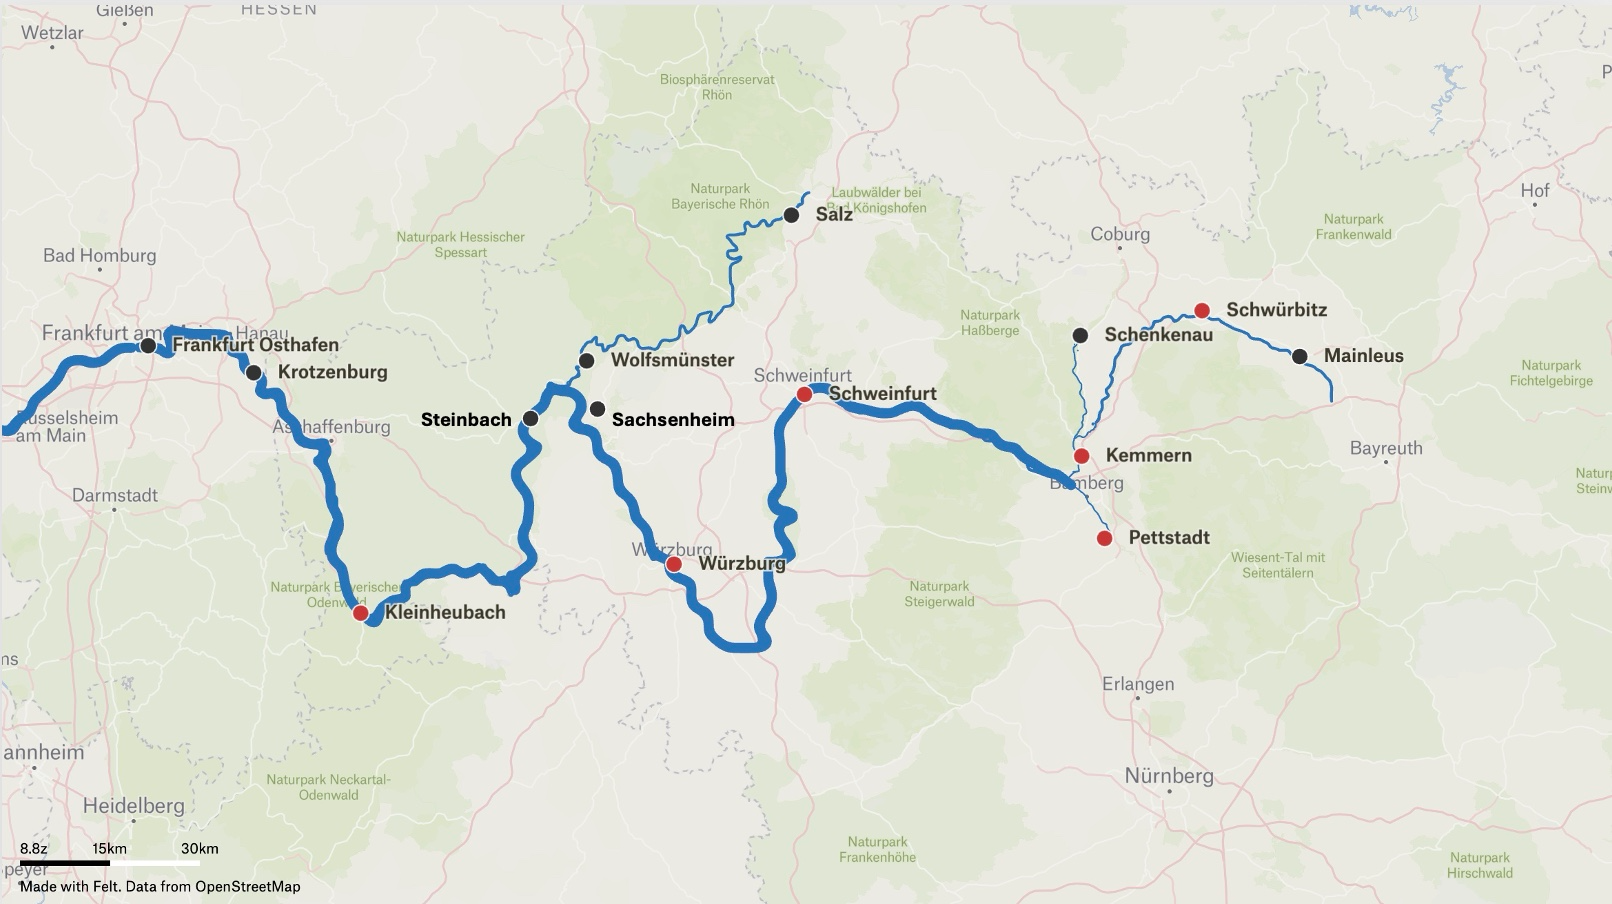
\includegraphics[width=0.8\linewidth]{work/05-riverine_heat/figures/05-stations_map} 

}

\caption{Map of Main river systen. The station included in the analysis are marked red.}\label{fig:rh-stations-map}
\end{figure}

\section{Methods}\label{methods-3}

\subsection{Threshold}\label{threshold}

The threshold which classifies riverine heatwaves has to be precisely defined. This paper uses the definition
of marine heatwaves by Hobday. Although it was originally defined for marine heatwaves, it has since been used on many
different studies about riverine heatwaves as well.

The definition of marine heatwaves by Hobday uses a 90th percentile seasonally varying threshold, which is also varying
with location and therefore calculated separately for each station. To calculate the seasonally varying threshold, for
each day the historical temperature measurements, as well as the historical measurements from a 11 day surrounding
window are taken. From these data points, the 90 percent quantile is taken. The exact formula for this calculation is
depicted below, where y is the year variable, d is the day variable and j is the day for the considered temperature \eqref{eq:rh-threshold}. \(Y_s\) and \(y_e\) are the years that mark the beginning and end of the baseline period, \(P_{90}(X)\) is the 90 percent
quantile of \(X\) . This procedure will be repeated for each day of year, until the threshold for the entire year is
completed \citep{hobday2016}.

\begin{equation}
T_{90}(j) = P_{90}(X),
\quad \text{where}
\quad
X = \left\{T(y,d)\;\middle|\; y_s \le y \le y_e,\; j-5 \le d \le j+5 \right\}
\label{eq:rh-threshold}
\end{equation}

Usually, for this a historical baseline period is used. But since here the data set only covers a relatively short time
period, the same time period was used for the calculation of the threshold and the analysis. Even if the same threshold
definition is used, comparing results from different studies on riverine heatwaves has to be treated carefully. It can
be problematic to compare exact numbers for metrics between studies with different baseline periods, as climate change
suggests a temperature biased over time. However, as in this paper the focus is only to demonstrate how heatwaves evolve
relatively to another over time by looking for general trends rather than comparing exact metrics with other studies.
And since in this paper only measurements from the same stations with the same baseline period were compared, this
approach also suffices.

Resulting from this procedure, for each station a threshold is obtained, that can be used for comparison with the time
series of each year. In figure \ref{fig:rh-threshold-kemmern} an example of this is shown for the Kemmern station and the
year 2018. Heatwaves can then be detected, by firstly marking all potential candidates, which are all days exceeding the
thresholds. After, the time series are examined for events of at least five consecutive days exceeding the threshold.
These are marked as heatwaves and given an ID, while all shorter events are discarded. When there is a gap of only one
or two days between two or more heatwaves that have a duration of at least five days each, the heatwaves, are
merged into one heatwave.

\subsection{Threshold example: Main data (Kemmern, 2018)}\label{threshold-example-main-data-kemmern-2018}

\begin{figure}

{\centering 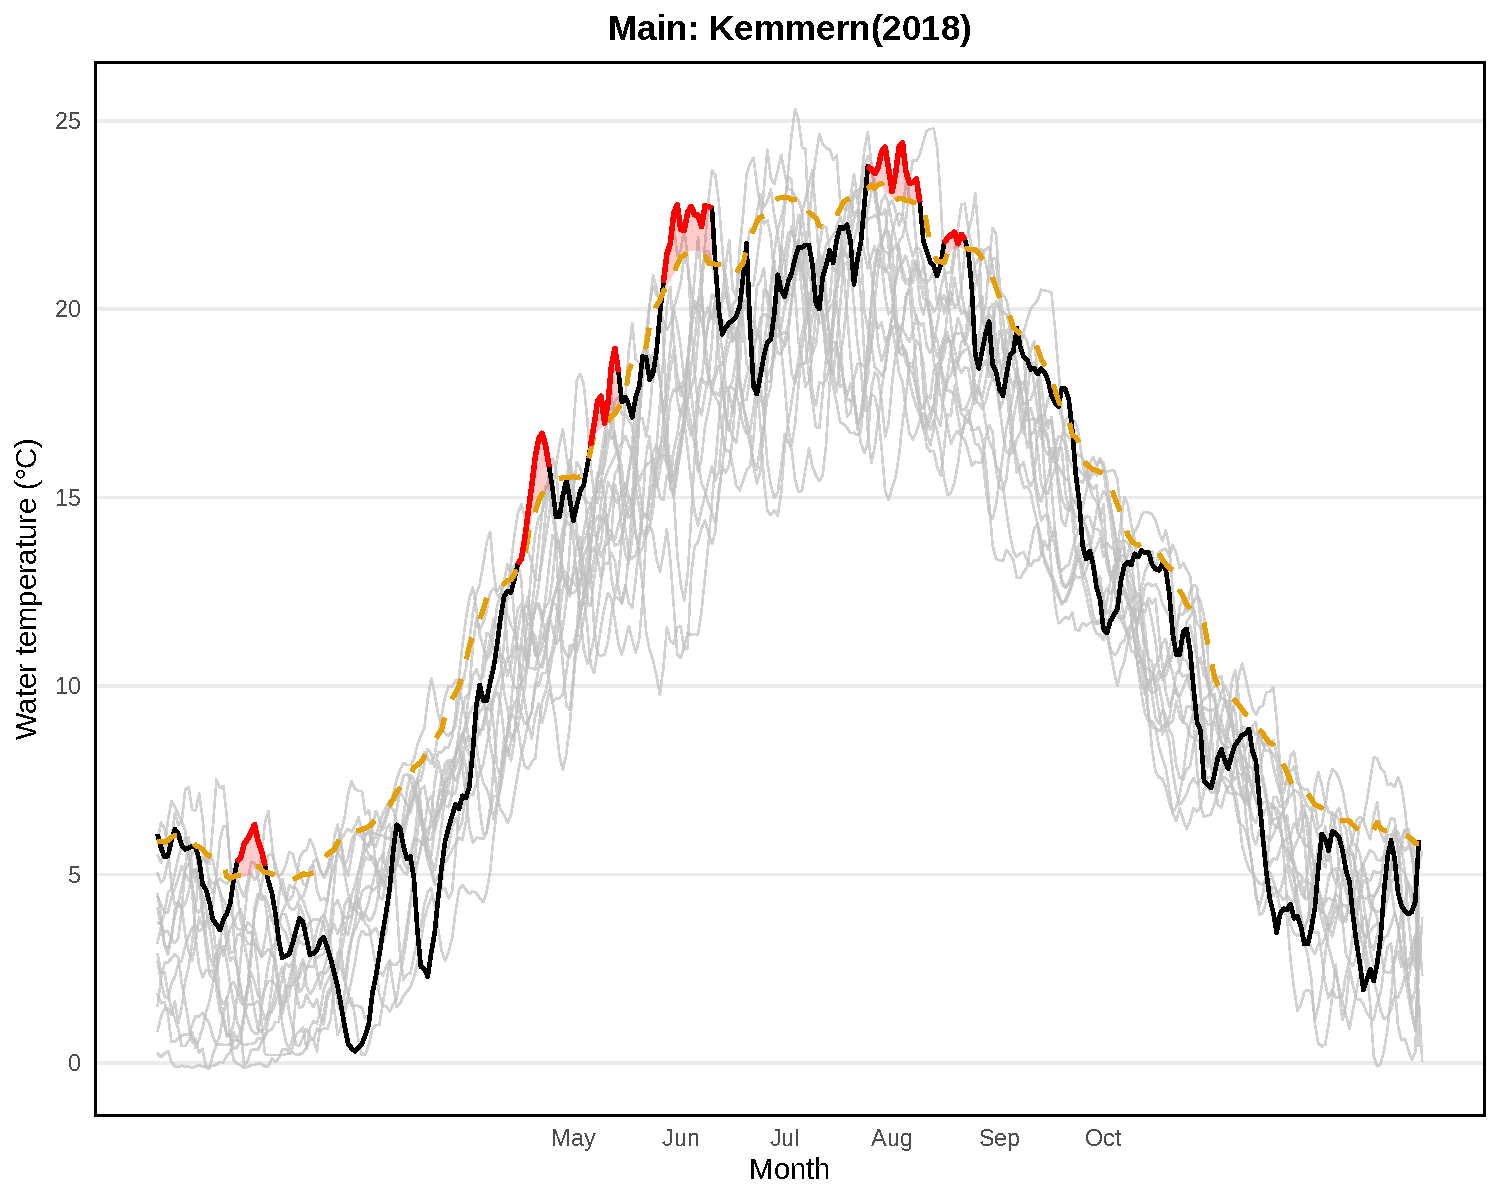
\includegraphics[width=0.7\linewidth]{work/05-riverine_heat/figures/05-threshold_kemmern} 

}

\caption{Temperature time series for Main Kemmern in 2018 (black line). The dotted orage line represents the heatwave threshold for Kemmern station. The red areas mark heatwaves in that year for Kemmern station. The light grey lines represent all temperature time series of Kemmern station for the baseline period.}\label{fig:rh-threshold-kemmern}
\end{figure}

\subsection{Metrics used}\label{metrics-used}

This paper focuses on three primary metrics, that are used to quantify the evolution of riverine heatwaves. A frequency
metric, a duration metric and an intensity metric were used, to describe the evolution under different aspects.

To quantify the evolution of frequency the number of heatwave events per year is used. For this, the number of different
heatwaves IDs are being counted per year and station.

Furthermore, the duration of a heatwave is considered. This is calculated using the first and last day of each
heatwave \eqref{eq:rh-duration} \citep{hobday2016}. The duration plays an important role, as especially longer heatwaves can have more severe
impacts.

\begin{equation}
D = t_e - t_s
\label{eq:rh-duration}
\end{equation}

Lastly, intensity is used, to assess the amount of the heat spike. The original definition by Hobday suggests to to define it as the temperature by which the climatological mean is exceeded. However, most literature on riverine heatwaves define intensity as the exceendance of the 90th percentile threshold \citep{sadayappan2025} \citep{chen2026}. Therefore this was also adopted for this paper. Also in this paper intensity is defined, as the mean of the daily temperature exceedance per heatwave\eqref{eq:rh-intensity}.

\begin{equation}
i_{\mathrm{mean}}
=
\overline{T(t)-T_{90}(j)}
\label{eq:rh-intensity}
\end{equation}

These metrics can also be used to summarize two or more of these characteristics. For example, the heatwave events can
be multiplied with the mean annual duration, to obtain the number of heatwave days per year. Or the duration of a
heatwave can be multiplied with its mean intensity, to obtain its mean severity.

\subsection{Research Question}\label{research-question}

This paper examines the evolution of riverine heatwaves during climate change. Therefore, its focus lies primarily on the development of the three previously defined metrics over time by posing the following questions:

\begin{enumerate}
\def\labelenumi{\arabic{enumi}.}
\item
  How has the frequency of riverine heatwaves changed over time?
\item
  How has the duration of riverine heatwaves changed over time?
\item
  How has the intensity of riverine heatwaves changed over time?
\end{enumerate}

Given the availability of stations with different locations along the same river system, it was also looked into how
the metrics differ between the stations. To answer these research questions, an exploratory analysis was performed
on the heatwave data, examining it for differences between stations and years. Also linear and quasi poisson modells
were fitted on the data, to look for significant temporal and spatial trends.

\section{Results}\label{results-3}

\subsection{Frequency}\label{frequency}

Figure \ref{fig:rh-heatwave-events-overview} shows the distribution of the number of heatwave events per year for each
station, with the stations being ordered by their position along the river from downstream to upstream. The plot shows, that
for each station the mean number of heatwave events lies between 2.5 and 3. Both its mean and its variance seem to
slightly increase in a downstream direction. To investigate this more thoroughly, a linear model between the mean
number of heatwave events per station, and the river kilometer was used. The river kilometer is a static variable that describes, the stations distance to the river mouth in kilometers. The model indicated a decreasing, however insignificant trend of -0.001935 events / year
with a p value of 0.197. As Pettstadt station lies on an inflow river and not directly on Main, it was excluded from
this model.

To examine the temporal trend of frequency, the heatwave events were grouped by their station, and a quasi poisson model
was used, to look for correlation between the frequency and year. Fitting a model for each individual station led only
to 1 significant and 5 insignificant results. Furthermore a common temporal trend quasi poisson model of frequency and
year was used, to examine the general temporal frequency trend. An analysis-of-deviance F-test was used to assess
whether including a year x station interaction significantly improved the quasi poisson model compared with a model
containing only year and station main effects. The year × station interaction did not significantly improve model fit (analysis of deviance F-test: F(5, 78) = 0.737, p = 0.598), indicating no statistical evidence that temporal trends
differed among stations.Therefore, the model with station as a fixed effect and a common temporal trend was used for the
analysis.
This resulted into a significant positive trend over time (slope: 0.05350, p value : 0.002), which indicates an increase
of heatwave events by 5.5 \% per year. The common quasi poisson is depicted in figure \ref{fig:rh-heatwave-events-plot}
where it is plotted into the frequency distribution of each station individually. The offset represents the intercept of
the station effect, as the frequency of heatwaves differs from station to station.

\begin{figure}

{\centering 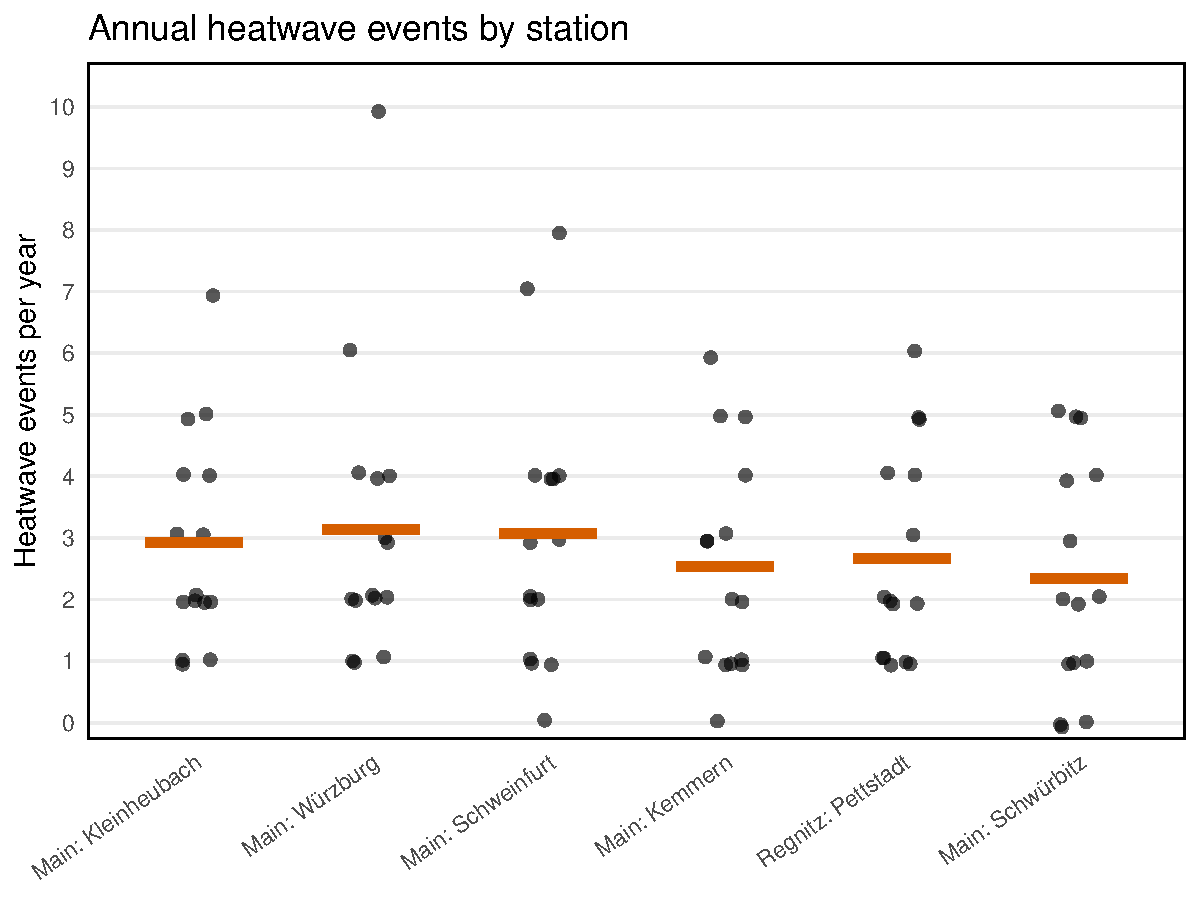
\includegraphics[width=0.8\linewidth]{work/05-riverine_heat/figures/05-heatwave_events_overview} 

}

\caption{Frequency distribution over all stations. The orange square signifies station mean value.}\label{fig:rh-heatwave-events-overview}
\end{figure}

\begin{figure}

{\centering 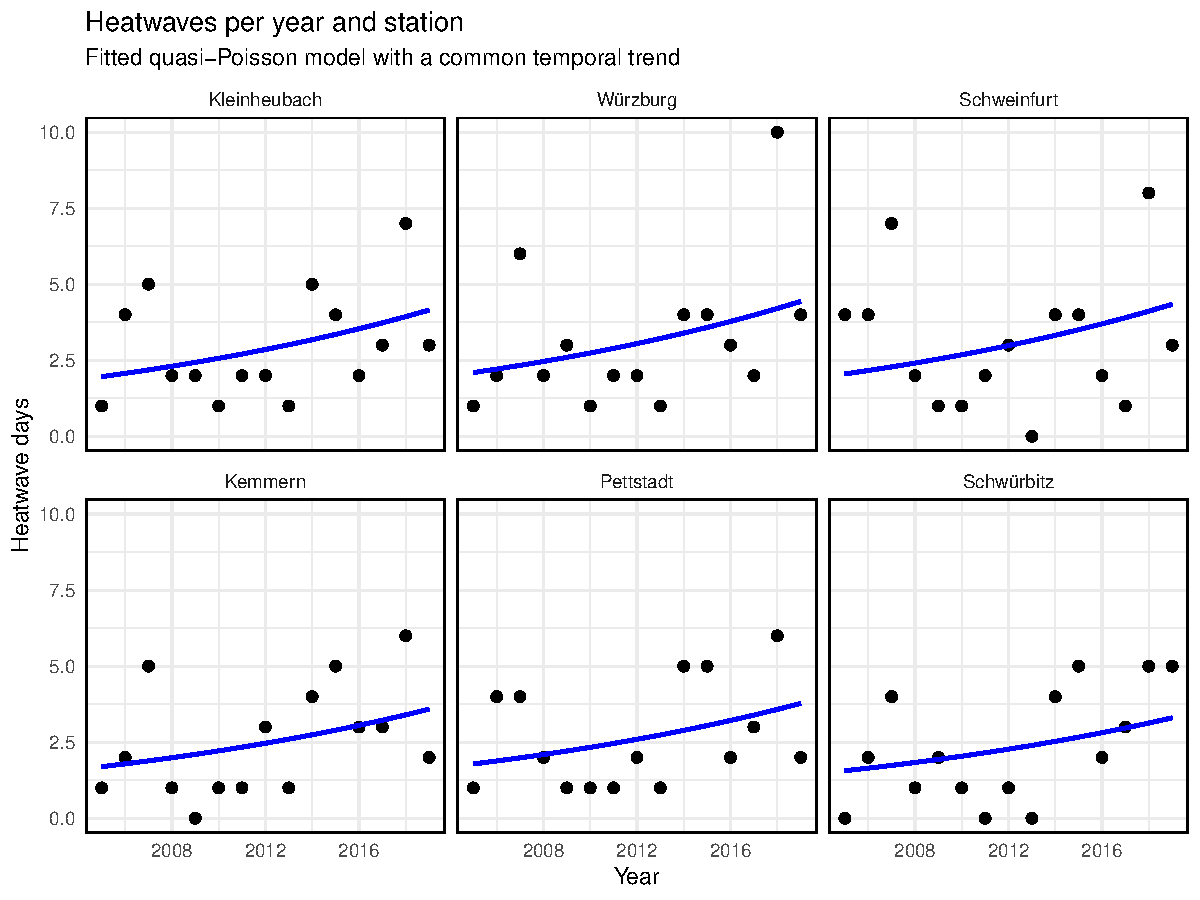
\includegraphics[width=0.8\linewidth]{work/05-riverine_heat/figures/05-heatwave_events_plot} 

}

\caption{Temporal development of heatwave events by station. The blue line shows the common temporal trend quasi poisson model.}\label{fig:rh-heatwave-events-plot}
\end{figure}

\subsection{Duration}\label{duration}

The durations of heatwaves of Main river in the considered period lay between 5 and 28, with averages between 8 and
10 days. Again the stations were placed according to their order along the
river, and while the mean stays consistent, the variance seems to increase downstream \ref{fig:rh-mean-duration-overview}. Also extremely long heatwaves
seem more common at the downstream stations. Again there was a model fitted between the mean duration of each station
and the river kilometer, this time a linear model was used, however it showed no significant trend
(slope: -0.002058 days / km, p value: 0.459). Another idea would be to examine the mean of the yearly maximum duration
of each station and look for a downstream trend. However, for this data set, this approach also did not deliver a
significant result (slope: -0.002475 days / km, p value: 0.616 ).

For the temporal trend a similar approach was used. The yearly mean durations for each station were plotted \ref{fig:rh-duration-plot}, and for each a linear model was fitted. Four of the six stations showed a positive trend, with only one of them being
significant, while the other stations showed a insignificant negative trend. To fit a linear model for the common
temporal duration trend, again the model with year x station interaction was tested against the model including only the
main effects, analogously to the frequency trend, this time using a analysis of variance F-Test. Again there was no indication for significantly differing trends between station, therefore the model with only the main effects was chosen. This resulted in a increasing, however insignificant, temporal trend of duration (slope: 0.08490 days / year, p value: 0.217).

\begin{figure}

{\centering 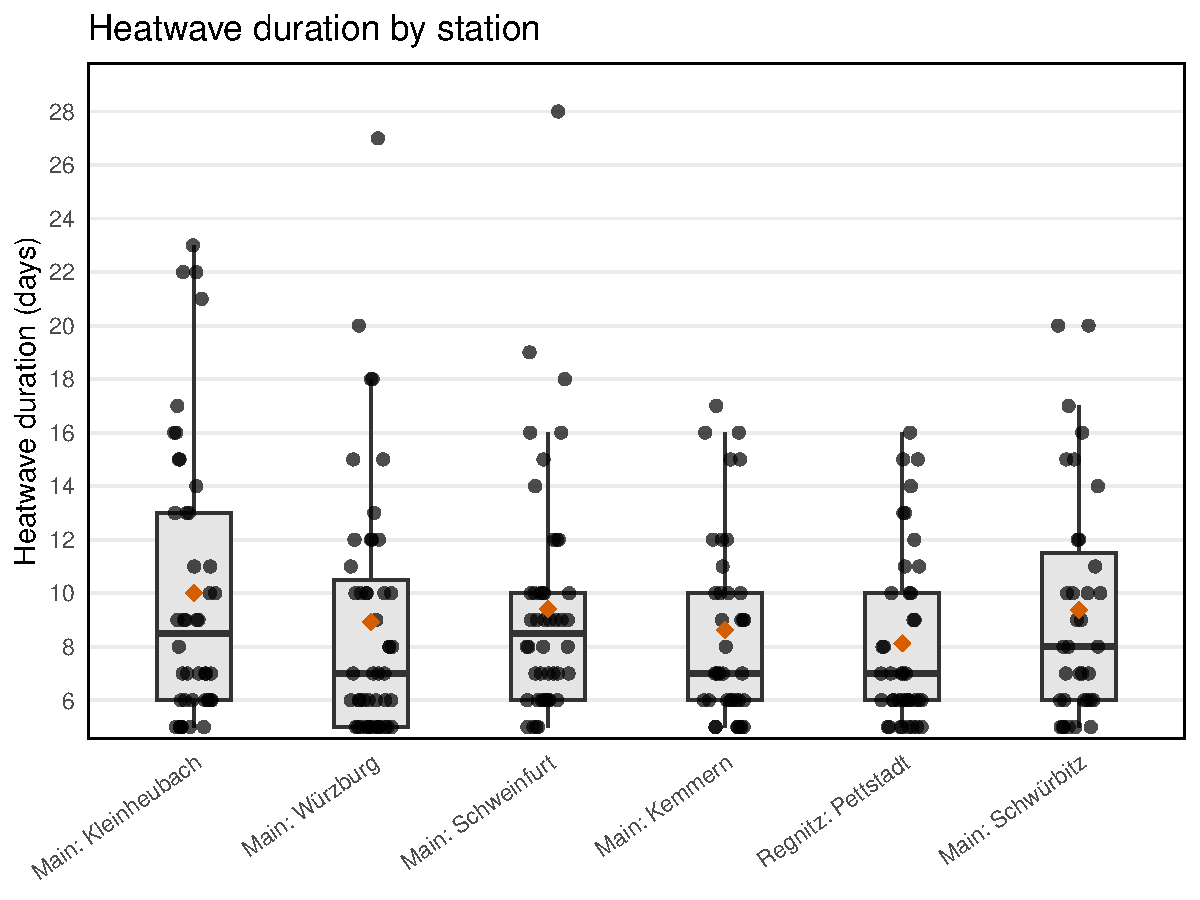
\includegraphics[width=0.8\linewidth]{work/05-riverine_heat/figures/05-mean_duration_overview} 

}

\caption{Distribution of mean duration for all stations. Each point signifies a single heatwave. The orange square signifies the average duration per station.}\label{fig:rh-mean-duration-overview}
\end{figure}

\begin{figure}

{\centering 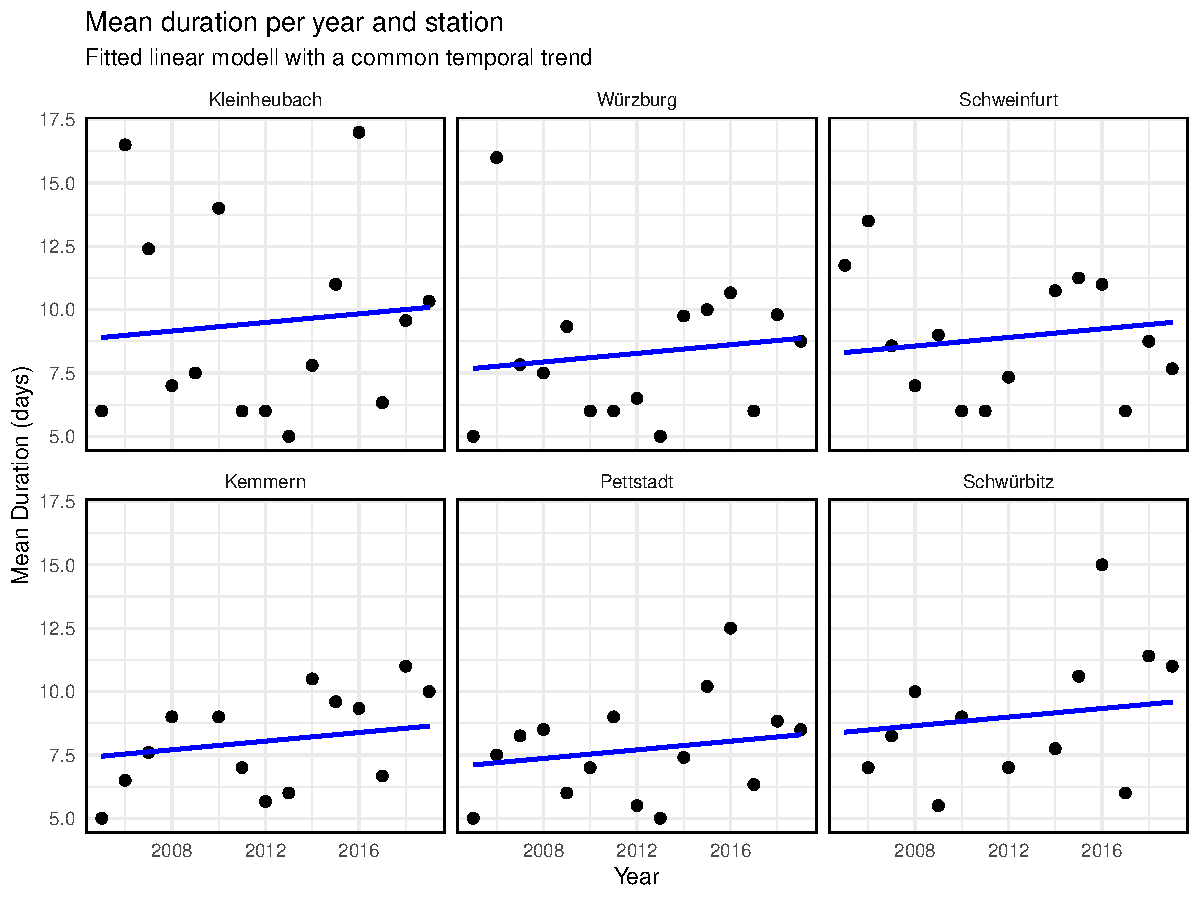
\includegraphics[width=0.8\linewidth]{work/05-riverine_heat/figures/05-duration_plot} 

}

\caption{Temporal development of mean heatwave duration by station. Each point signifies the annual mean duration for the considered station. The blue line shows the common temporal trend linear model.}\label{fig:rh-duration-plot}
\end{figure}

\subsection{Intensity}\label{intensity}

The intensity lies between 0 and 2 degrees celsius over the threshold, with the stations means laying between 0.5 and
0.8 degrees Celsius. Again the plot \ref{fig:rh-mean-intensity-overview} suggests a trend between the location of the
stations, it seems like the mean intensity and its variance decrease stream downwards. To capture this trend, a linear
model was used, which gave a slope of 0.0011531 °C per km, however again this result was not significant for the 95
percent confidence level with a p value of 0.059.

Looking at the yearly data \ref{fig:rh-intensity-plot}, the plots again reflect the higher variance for upstream stations
Schwürbitz, Schweinfurt and Kemmern, however a clear temporal trend is not visible. Also neither the station specific
linear models, nor the common temporal trend model showed a significant trend. The result of the common model was a slope 0.008265 °C per year with a p value of 0.187, while the individual models showed no significant trend for any of the stations. The common temporal trend model was fitted and tested analogously to the model for duration.

\begin{figure}

{\centering 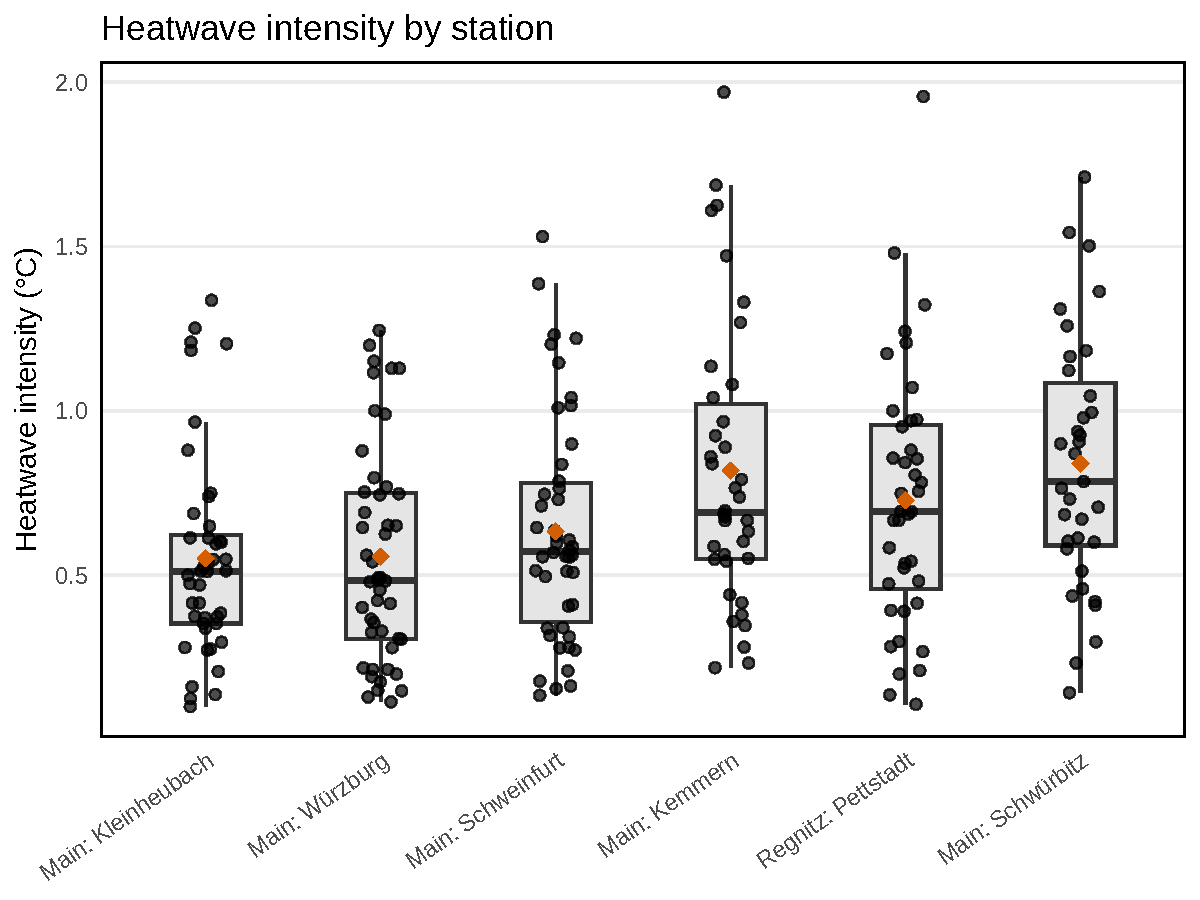
\includegraphics[width=0.8\linewidth]{work/05-riverine_heat/figures/05-mean_intensity_overview} 

}

\caption{Distribution of heatwave intensity by station. Each point represents the intensity of one heatwave. The orange square signifies the mean heatwave intensity for each station}\label{fig:rh-mean-intensity-overview}
\end{figure}

\begin{figure}

{\centering 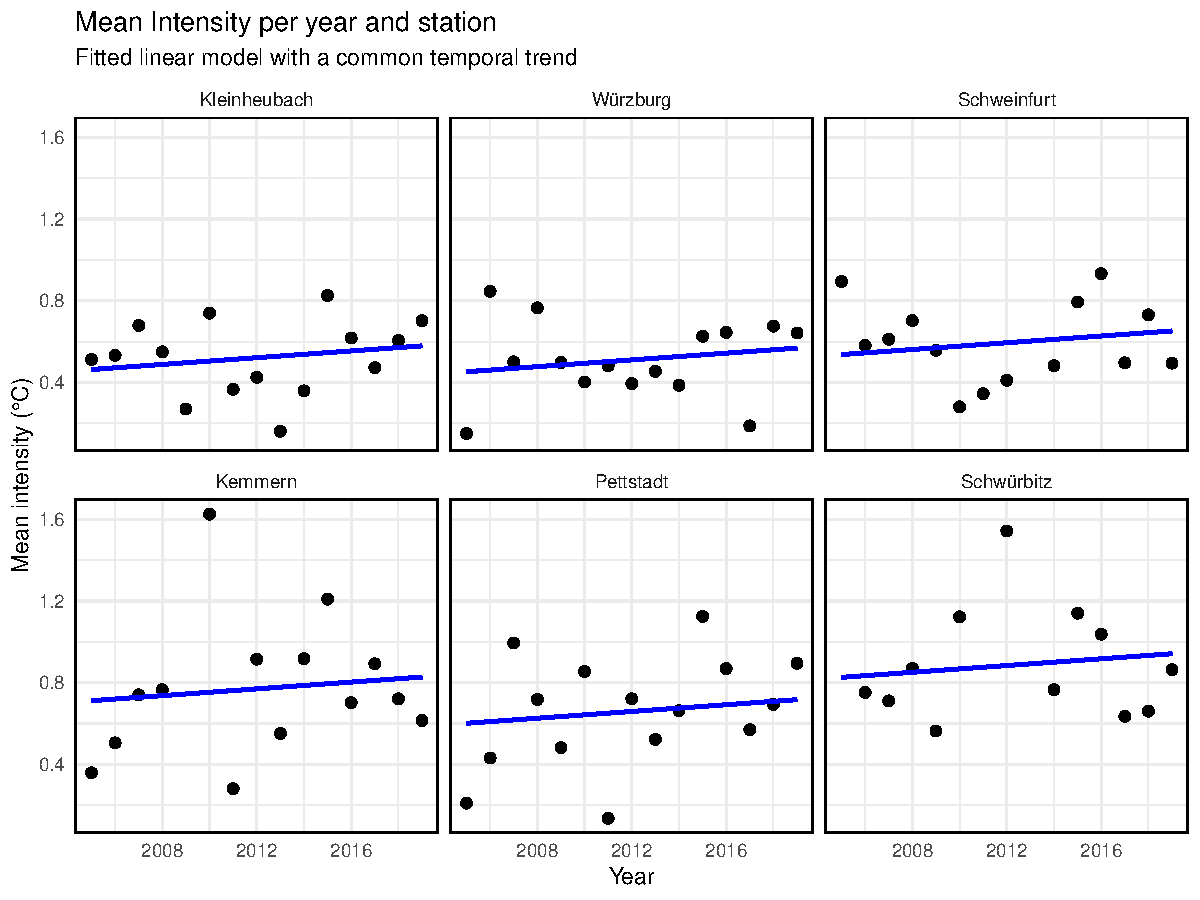
\includegraphics[width=0.8\linewidth]{work/05-riverine_heat/figures/05-intensity_plot} 

}

\caption{Temporal development of mean heatwave intensity by station. Each point signifies the annual mean heatwave intensity for the considered station. The blue line shows the common temporal trend linear model.}\label{fig:rh-intensity-plot}
\end{figure}

\section{Discussion}\label{discussion-2}

\subsection{Overview of trends common models}\label{overview-of-trends-common-models}

\begin{figure}

{\centering 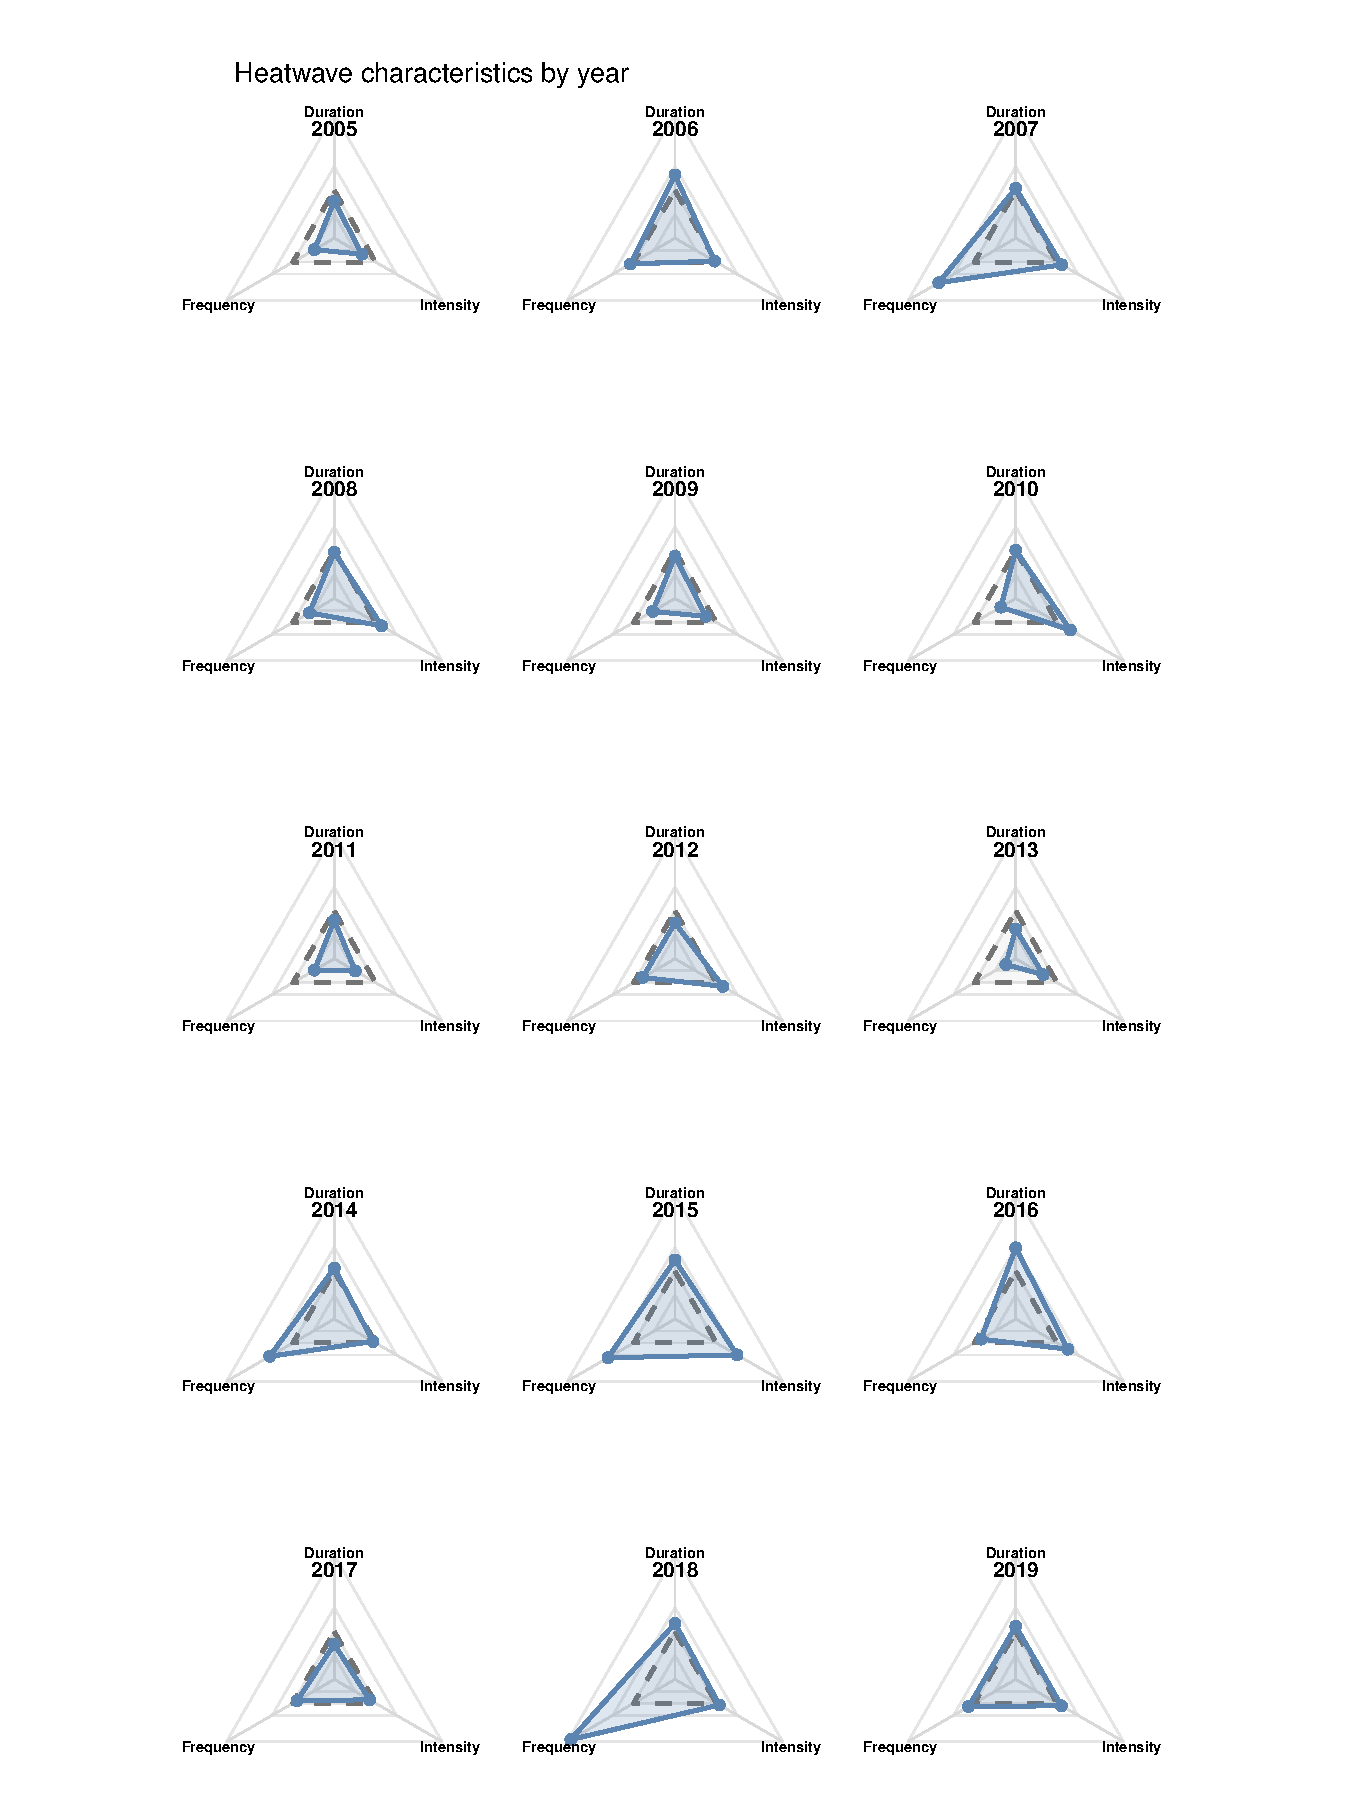
\includegraphics[width=0.8\linewidth]{work/05-riverine_heat/figures/05-polygon_temporal} 

}

\caption{All three heatwave metrics by year. Values are expressed relative to the mean across years (1.0 = overall mean); the dashed grey triangle indicates the overall mean.}\label{fig:rh-polygon-temporal}
\end{figure}

The observed results of all three metrics are summarized for the temporal trends in figure \ref{fig:rh-polygon-temporal}
and for the differences between stations in figure \ref{fig:rh-polygon-spatial}. From the literature a increasing trend
over time for all three metrics would be expected \citep{chen2026} \citep{sadayappan2025}. This analysis only reflects a significant increasing trend for
frequency, while duration and intensity also show increasing, but insignificant trends. However, the recommended data
size of time series with a length of ideally at least 30 years were not met, as only a period of 15 years was
considered. Also there was no historical period used to calculate the heatwave threshold. This might explain the
insignificance of the duration and intensity trend. Moreover, only data from one river was considered, and a trend of
one river does not necessarily match the global trend of riverine heatwave increase. With a longer time series it might
be possible to obtain significant results for the temporal trends of duration and intensity, or it might be possible to
have a larger confidence that there is no significant temporal trend for these metrics in Main river system.

However, finding usable data for the analysis of riverine heatwaves is difficult, as due to the suspected climate
change bias it is not always reasonable to use a long period of historical data as a baseline. With the temperatures
being in general a lot higher than in the past, a historical threshold would not be able to capture heatwaves anymore,
as a too large amount of temperatures would exceed it. Leading to permanent heatwave states, which would make the
examination of frequency and duration meaningless, and a temporal trend would not be able to be detected. An idea to
account for the temporal bias in temperature data would be to use simulated data. By using simulated data, longer time
series could be used, the climate change bias would be incorporated in the threshold calculation, and predictions for
future development of riverine heatwaves would be possible.

\begin{figure}

{\centering 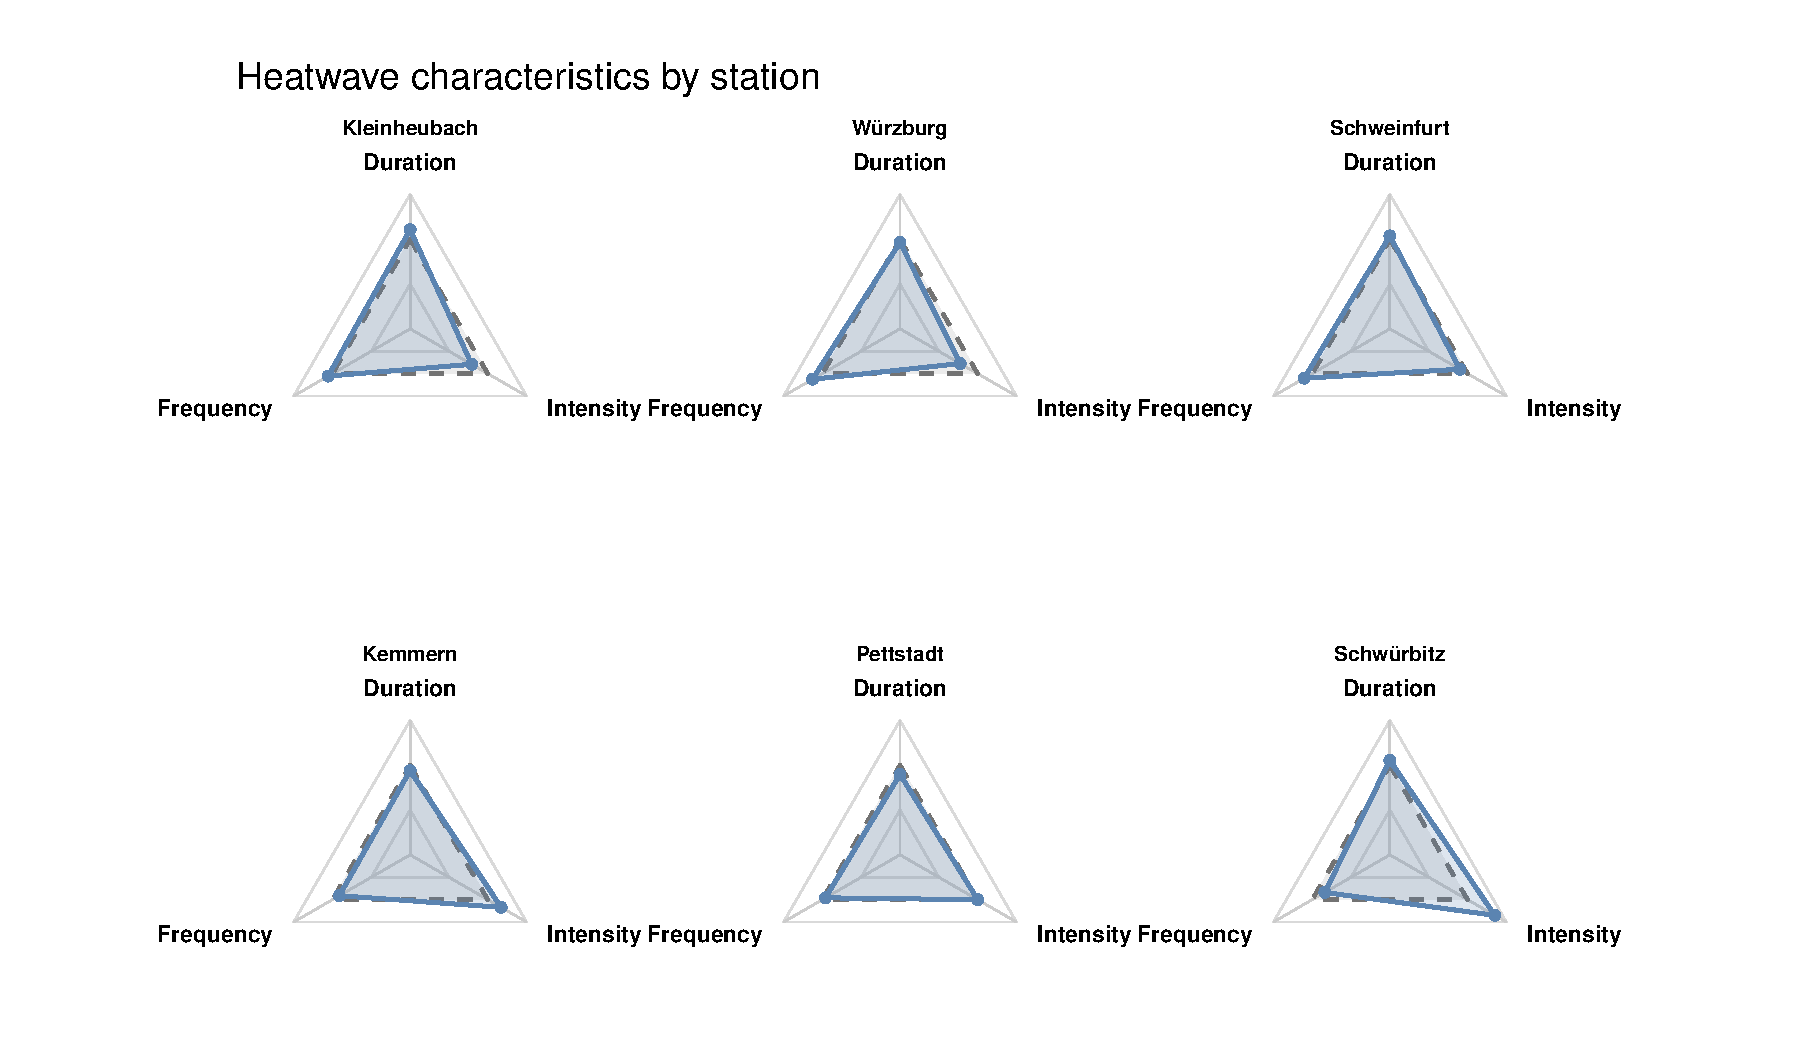
\includegraphics[width=\linewidth]{work/05-riverine_heat/figures/05-polygon_spatial} 

}

\caption{All three heatwave metrics by station. Values are expressed relative to the mean across all stations (1.0 = overall mean); the dashed grey triangle indicates the overall mean.}\label{fig:rh-polygon-spatial}
\end{figure}

The plots indicated, that there was a correlation between frequency and intensity and the river kilometer. The
implication was, that the frequency of heatwaves increase downstream ward, while their intensity decreases. These trends
however could not be verified using linear models, which did not deliver significant results. However, it could be
interesting to perfom further examinations on this trends, using longer time series, or a larger number of stations along
the same river, maybe also on a different river with a denser network of gauges. The frequency trend might indicate,
that there is a downstream movement of riverine heatwaves, that might explain the higher frequency downstream wards.
This could be interesting to make predictions on the appearance of heatwaves downstreams, after one has appeared further
upstream.

The results, in a way, show the difficulties of data scarcities when working on temporal trend analysis with riverine
heatwaves during climate change. This underlines the importance of constructing a dense network of temperature data,
perhaps with the help of simulated data. Although a significant temporal trend was only detected for frequency, there
were some implications for increasing trends from the other metrics, which, as potential trends between the river
kilometer and frequency and intensity, might be an interesting relation to examine in a larger data set. In conclusion
riverine heatwaves remain a relevant phenomenon, during climate change, that still offers many interesting research
possibilities.

\chapter{Interpretable Riverine Heatwaves}\label{irh}

\emph{Author: }

\emph{Supervisor: Henri Funk}

\emph{Degree: Bachelor/Master}

\section{Abstract}\label{abstract-3}

Lorem ipsum dolor sit amet, consectetur adipiscing elit. Sed do eiusmod tempor incididunt ut labore et dolore magna aliqua. Ut enim ad minim veniam, quis nostrud exercitation ullamco laboris nisi ut aliquip ex ea commodo consequat. Duis aute irure dolor in reprehenderit in voluptate velit esse cillum dolore eu fugiat nulla pariatur. Excepteur sint occaecat cupidatat non proident, sunt in culpa qui officia deserunt mollit anim id est laborum.

\section{Introduction}\label{introduction-4}

\chapter{Changepoint analysis is statistics}\label{cs}

\emph{Author: }

\emph{Supervisor: Helmut Küchenhoff}

\emph{Degree: Bachelor/Master}

\section{Abstract}\label{abstract-4}

Lorem ipsum dolor sit amet, consectetur adipiscing elit. Sed do eiusmod tempor incididunt ut labore et dolore magna aliqua. Ut enim ad minim veniam, quis nostrud exercitation ullamco laboris nisi ut aliquip ex ea commodo consequat. Duis aute irure dolor in reprehenderit in voluptate velit esse cillum dolore eu fugiat nulla pariatur. Excepteur sint occaecat cupidatat non proident, sunt in culpa qui officia deserunt mollit anim id est laborum.

\section{Introduction}\label{introduction-5}

\chapter{Uncertainty of tipping points in climate research}\label{utp}

\emph{Author: }

\emph{Supervisor: Helmut Küchenhoff}

\emph{Degree: Bachelor/Master}

\section{Abstract}\label{abstract-5}

Lorem ipsum dolor sit amet, consectetur adipiscing elit. Sed do eiusmod tempor incididunt ut labore et dolore magna aliqua. Ut enim ad minim veniam, quis nostrud exercitation ullamco laboris nisi ut aliquip ex ea commodo consequat. Duis aute irure dolor in reprehenderit in voluptate velit esse cillum dolore eu fugiat nulla pariatur. Excepteur sint occaecat cupidatat non proident, sunt in culpa qui officia deserunt mollit anim id est laborum.

\section{Introduction}\label{introduction-6}

\chapter{Tipping Points in Climate Research: An Overview}\label{tp-overview}

\emph{Author: Chengyuan Ou}

\emph{Supervisor: Prof.~Dr.~Helmut Küchenhoff}

\emph{Degree: Bachelor}

\section{Abstract}\label{abstract-6}

A climate tipping point is a critical threshold beyond which a component of
the Earth system shifts into a qualitatively different state, often abruptly
and with limited reversibility. This chapter reviews the definition of
tipping points, summarises the 16 major tipping elements assessed by
\citet{armstrongmckay2022}, and outlines how their temperature thresholds are
estimated and why those estimates remain uncertain. It then turns to Early
Warning Signals (EWS): statistical indicators based on critical slowing
down that can be computed from observed time series without prior knowledge
of the threshold. The approach is illustrated for the Central-Western
Greenland ice sheet by reproducing the statistical analysis of \citet{boers2021}
from the authors' publicly released data. The chapter ends with the main
limitations of EWS, following \citet{rietkerk2025}.

\section{Introduction}\label{introduction-7}

The term ``tipping point'' entered climate science when \citet{lenton2008} used it
for large Earth-system components---tipping elements---that can be driven
past a critical threshold by anthropogenic warming. Once the threshold is
crossed, the system may change state on a timescale short relative to the
forcing, and the change may be hard or impossible to reverse. Because such
transitions would affect sea level, regional climate and ecosystems,
identifying tipping elements, estimating their thresholds and monitoring
their approach have become central research questions.

Section \ref{tp-definition} states a formal definition. Section
\ref{tp-elements} summarises the 16 tipping elements currently assessed
in the literature. Section \ref{tp-thresholds} covers threshold estimation and the main
sources of uncertainty. Section \ref{tp-ews}
introduces the statistical theory of Early Warning Signals, and Section
\ref{tp-case} applies it to Central-Western Greenland, including an
independent reproduction of the statistical analysis. Section
\ref{tp-limits} discusses the limitations of the EWS approach.

\section{Definition of a Climate Tipping Point}\label{tp-definition}

\citet{lenton2008} define a tipping element as a climate subsystem with a critical
threshold in some control parameter \(\rho\), such that a small push beyond
that threshold produces a disproportionately large change in a system
feature \(F\). Formally, a tipping transition occurs if, for a given time
horizon \(T\),

\[
|F(\rho \geq \rho_{\text{crit}} + \delta\rho \mid T) - F(\rho_{\text{crit}} \mid T)| \geq \hat{F} > 0 ,
\]

where \(\rho_{\text{crit}}\) is the critical value of the control parameter,
\(\delta\rho\) an arbitrarily small excess forcing, and \(\hat{F}\) a change in
\(F\) that is large relative to ordinary variability.

The system can be thought of as starting in a stable state A. As \(\rho\)
increases past \(\rho_{\text{crit}}\), state A loses stability and the
system moves, often rapidly, into an alternative stable state B. For most
of the elements discussed below, Global Mean Surface Temperature (GMST)
above pre-industrial levels is used as the control parameter. GMST does
not act directly on every subsystem; it alters local temperature,
precipitation or salinity, which then drive the feature of interest (ice
volume, forest cover, overturning strength, and so on). Using GMST
nonetheless allows thresholds for physically very different systems to be
compared on a common scale.

\begin{figure}

{\centering 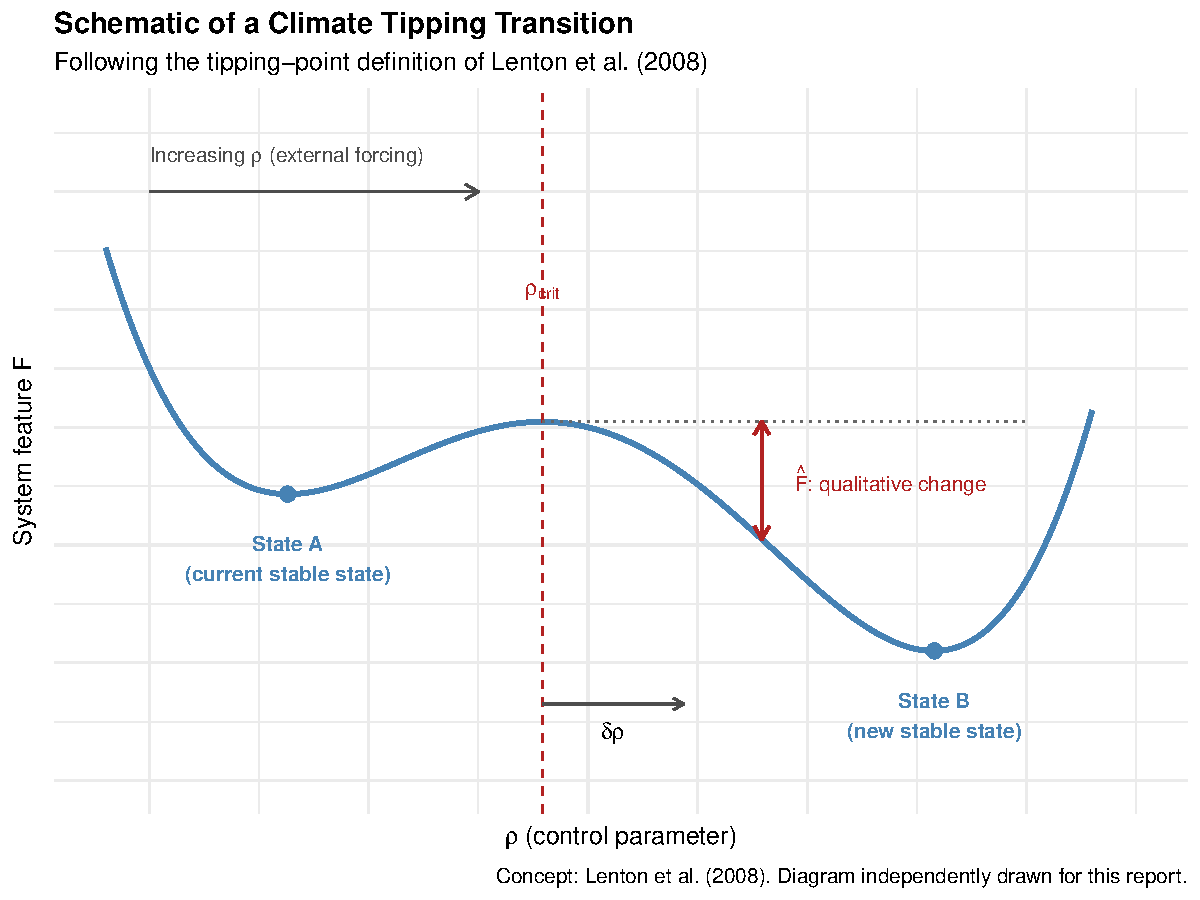
\includegraphics[width=0.85\linewidth]{work/09-tp-overview/figures/tp_tipping_point_schematic} 

}

\caption{Schematic of a climate tipping transition, following the tipping-point definition of Lenton et al. (2008).}\label{fig:tp-schematic}
\end{figure}

\section{Overview of the 16 Tipping Elements}\label{tp-elements}

\citet{armstrongmckay2022} identify 16 tipping elements and give temperature
thresholds relative to pre-industrial levels. The elements span several
geographical domains: the Greenland and Antarctic ice sheets; Atlantic
overturning and subpolar convection; the Amazon basin; Arctic sea ice and
boreal permafrost and forest; tropical coral reefs; mountain glaciers; and
the West African monsoon. They are grouped by the spatial scale of their
expected impacts.

\textbf{Global core} elements are those whose tipping would have severe effects
well beyond the region of origin, for example through multi-metre sea-level
rise or large-scale disruption of atmospheric circulation (Table
\ref{tab:tp-elements-global}).

\begin{table}[!h]
\centering
\caption{\label{tab:tp-elements-global}Global core tipping elements and their estimated temperature thresholds above pre-industrial levels. Source: Armstrong McKay et al. (2022), Table 1.}
\centering
\resizebox{\ifdim\width>\linewidth\linewidth\else\width\fi}{!}{
\begin{tabular}[t]{lll}
\toprule
Element & Dynamics & Threshold range (°C)\\
\midrule
Greenland Ice Sheet & Collapse & 0.8 - 3.0\\
West Antarctic Ice Sheet & Collapse & 1.0 - 3.0\\
Labrador-Irminger Seas / SPG Convection & Collapse & 1.1 - 3.8\\
Atlantic Meridional Overturning Circulation (AMOC) & Collapse & 1.4 - 8.0\\
Amazon Rainforest & Dieback & 2.0 - 6.0\\
\addlinespace
Boreal Permafrost & Collapse & 3.0 - 6.0\\
East Antarctic Subglacial Basins & Collapse & 2.0 - 6.0\\
Arctic Winter Sea Ice & Collapse & 4.5 - 8.7\\
East Antarctic Ice Sheet & Collapse & 5.0 - 10.0\\
\bottomrule
\end{tabular}}
\end{table}

\textbf{Regional-impact} elements mainly affect the region in which they are
located (Table \ref{tab:tp-elements-regional}). Boreal permafrost
appears in both tables because \citet{armstrongmckay2022} distinguishes two modes:
gradual collapse with large carbon release (global core) and abrupt thaw
with more localised impacts (regional). The temperature ranges therefore
refer to different processes, not to a duplicated entry.

\begin{table}[!h]
\centering
\caption{\label{tab:tp-elements-regional}Regional-impact tipping elements and their estimated temperature thresholds above pre-industrial levels. Source: Armstrong McKay et al. (2022), Table 1.}
\centering
\resizebox{\ifdim\width>\linewidth\linewidth\else\width\fi}{!}{
\begin{tabular}[t]{lll}
\toprule
Element & Dynamics & Threshold range (°C)\\
\midrule
Low-latitude Coral Reefs & Die-off & 1.0 - 2.0\\
Boreal Permafrost & Abrupt thaw & 1.0 - 2.3\\
Barents Sea Ice & Abrupt loss & 1.5 - 1.7\\
Mountain Glaciers & Loss & 1.5 - 3.0\\
Sahel and West African Monsoon & Greening & 2.0 - 3.5\\
\addlinespace
Boreal Forest (south) & Dieback & 1.4 - 5.0\\
Boreal Forest (north) & Expansion & 1.5 - 7.2\\
\bottomrule
\end{tabular}}
\end{table}

The 2015 Paris Agreement aims to keep global warming well below 2°C above
pre-industrial levels, and preferably to 1.5°C. Several estimated threshold
ranges in the tables above already fall within or near this interval,
including those for the Greenland and West Antarctic ice sheets,
Labrador-Irminger Seas convection, low-latitude coral reefs and boreal
permafrost under abrupt thaw. Tipping risk is therefore already relevant at
warming levels still treated as policy targets.

\section{Threshold Estimation and Uncertainty}\label{tp-thresholds}

\subsection{Threshold estimation}\label{threshold-estimation}

The ranges in Tables \ref{tab:tp-elements-global} and
\ref{tab:tp-elements-regional} are not taken from a single study.
They are compiled from three types of evidence:

\begin{enumerate}
\def\labelenumi{\arabic{enumi}.}
\tightlist
\item
  \textbf{System-specific models}, which estimate when a given system loses
  stability (for example ice-sheet models for Greenland).
\item
  \textbf{Paleoclimate records}, which document system states at known past
  temperatures. For Greenland, the MIS-11 interglacial (about 400,000
  years ago) is a key reference: temperatures of roughly 1.5°C above
  pre-industrial levels coincided with substantially reduced ice extent.
\item
  \textbf{Theoretical constraints and earlier assessments}, carried over from
  previous reviews.
\end{enumerate}

Expert judgement then combines these sources into, for each element, a
maximum threshold, a best (``likely'') estimate and a minimum (``possible'')
threshold. The Greenland Ice Sheet illustrates the procedure. Model
estimates range from about 1.5--1.6°C \citep{robinson2012} to
\(2.7\pm0.2\)°C \citep{noel2021}, while MIS-11 evidence points near 1.5°C.
Putting these together yields a best estimate of 1.5°C and a plausible
range of 0.8°C to 3.0°C.

\subsection{Sources of uncertainty}\label{sources-of-uncertainty}

The spread of such estimates is large. Four sources of uncertainty are
particularly important:

\begin{itemize}
\tightlist
\item
  \textbf{Definitional differences.} Studies do not always use the same
  criterion for ``tipping'', nor do they always track the same system
  feature. Changing either can shift the reported threshold.
\item
  \textbf{Model and process representation.} Models differ in how they
  represent feedbacks such as ice-elevation feedback or ocean--atmosphere
  coupling, and therefore disagree on when stability is lost.
\item
  \textbf{Observational and paleoclimate constraints.} Proxies are sparse and
  indirect, and are subject to dating and interpretation error, so the
  past temperatures and ice extents used as anchors remain uncertain.
\item
  \textbf{Tipping cascades.} Elements are not independent. Collapse of AMOC,
  for example, could alter the effective threshold for the Amazon
  rainforest. Thresholds estimated for isolated systems should therefore
  be read as approximate, not as fixed values.
\end{itemize}

\section{Early Warning Signals (EWS)}\label{tp-ews}

Because exact thresholds are hard to pin down in advance, a parallel line
of work asks whether the approach of a tipping point can be seen in the
data themselves. The underlying idea is critical slowing down (CSD).

Near a tipping point, the dynamics of a feature \(x\) around its equilibrium
\(x^*\) can be approximated by the linear stochastic equation

\[
\frac{d(x - x^*)}{dt} = \lambda (x - x^*) + \eta(t),
\]

where \(\lambda < 0\) is the restoring rate and \(\eta(t)\) is stochastic
forcing. As the tipping point is approached, the restoring force weakens
and \(\lambda \to 0\). Two statistical consequences follow.

First, lag-1 autocorrelation (AC1) rises. Discretising the equation with
time step \(\Delta t\) yields an AR(1) process with coefficient

\[
\text{AC1} = \alpha = e^{\lambda \Delta t} \longrightarrow 1 \quad \text{as } \lambda \to 0,
\]

so past perturbations persist longer before the system relaxes.

Second, variance increases. Under the same approximation, the stationary
variance of fluctuations around equilibrium behaves as

\[
\sigma^2 \propto \frac{1}{1-\alpha^2} \longrightarrow \infty \quad \text{as } \alpha \to 1,
\]

so fluctuations accumulate rather than being damped.

In applications, both indicators are estimated in a sliding window on a
detrended series; a significant upward trend is then read as an early
warning signal \citep{rietkerk2025}. Section \ref{tp-case} applies this
procedure to observational melt data.

\section{Case Study: Central-Western Greenland Ice Sheet}\label{tp-case}

\subsection{Background}\label{background}

The Central-Western Greenland (CWG) sector lies on the western margin of
the Greenland Ice Sheet, where surface melt is strong and the
melt--elevation feedback is particularly relevant: lowering of the ice
surface exposes it to warmer air, which further increases melt. \citet{boers2021}
ask whether this region shows signs of approaching a tipping point.
Detrended CWG melt rates exhibit rising variance and lag-1 autocorrelation,
consistent with critical slowing down. Such trends alone could, however,
have other causes.

The authors therefore link the statistical signal to a physical mechanism.
They reconstruct the ice-sheet height anomaly \(\Delta h\) from the melt
series and fit a melt-elevation feedback (MEF) model,

\[
C \frac{d\Delta h}{dt} = -p_0 (\Delta h^m - p_1) + p_2 (\Delta h - p_1) - (T - p_3) + \eta(t),
\]

in which \(C\) is a heat-capacity factor, \(m\) a nonlinearity exponent,
\(T\) local summer temperature, and \(p_0,\dots,p_3\) fitted parameters that
control feedback strength. The reconstructed height tracks the model's
equilibrium closely (\(R^2 = 0.94\)), and the fluctuations around that
equilibrium behave as predicted: variance and autocorrelation both
increase with temperature.

The MEF model is not an independent second data set. It shows that the
rising variance and autocorrelation correspond to a weakening restoring
force as temperature rises---the mechanism CSD is meant to capture. The
reproduction below concerns only the statistical part of the argument: the
signal in the melt series itself.

\subsection{Data and Methods}\label{data-and-methods}

The analysis is reproduced in R from the melt record released with the
paper (\texttt{github.com/niklasboers/GrIS-EWS}, file
\texttt{CWG\_NU\_melt\_jja\_temp.txt}), covering the CWG stack melt series from 1650
to 2013. The original data are not stored in this repository; the
reproduction script reads them from the authors' public GitHub page.
Code is in \texttt{work/09-tp-overview/R/tp\_ews\_reproduction.R}.

As in the original study, the series is restricted to 1855--2013; earlier
years were excluded there as noisier and less reliable. The steps are as
follows.

\begin{enumerate}
\def\labelenumi{\arabic{enumi}.}
\item
  \textbf{Log-transformation.} Let \(m_t\) denote the CWG melt rate in year \(t\).
  Because melt rates vary over a large range, the analysis uses
  \(x_t = \log(m_t - \min_s m_s + 1)\). The shift keeps all arguments of the
  logarithm strictly positive; the transform reduces heteroscedasticity
  before detrending.
\item
  \textbf{Gaussian detrending.} A slow trend \(\tilde x_t\) is estimated by a
  Gaussian-weighted moving average of the neighbouring values of \(x_t\),
  with bandwidth \(\sigma = 30\) years:
  \[
  \tilde x_t = \sum_{k} w_k x_{t+k}, \qquad
  w_k \propto \exp\!\left(-\frac{k^2}{2\sigma^2}\right),
  \]
  after normalising the weights to sum to one. Near the ends of the
  record the series is reflected so that the smoother is well defined.
  The residual \(r_t = x_t - \tilde x_t\) is the detrended series used
  below; it isolates shorter-term fluctuations from the long-term
  warming-related rise in melt.
\item
  \textbf{Sliding-window estimation.} A trailing window of width \(w = 70\)
  years is used, consistent with \citet{boers2021} (Fig. 1 D/E). For each end
  year \(t\) for which the preceding \(w\) observations are available, the
  sample variance and the lag-1 autocorrelation of \(\{r_s\}\) are computed
  on \(\{r_{t-w+1},\ldots,r_t\}\). This yields two indicator series, one for
  variance and one for AC1, each indexed by the window end year.
\item
  \textbf{Trend estimation.} Each indicator series \(Y_t\) is modelled as
  \(Y_t = \beta_0 + \beta_1 t + \varepsilon_t\). The slope \(\beta_1\) is
  estimated by ordinary least squares (OLS) and measures the linear
  change of the indicator over the analysis period. Under standard
  regression assumptions, a \(t\)-test of \(H_0\!:\,\beta_1 = 0\) yields an
  associated \(p\)-value. Successive window estimates are serially
  dependent, so these \(p\)-values are reported as indicative. The
  parameter choices \(\sigma = 30\) and \(w = 70\) match one of the
  combinations shown in the main figure of \citet{boers2021}; that study also
  reports robustness for detrending bandwidths of 20--60 years and
  windows of 40--120 years, and assesses trend significance with a
  Fourier phase-surrogate test.
\end{enumerate}

\subsection{Results}\label{results-4}

\begin{figure}

{\centering 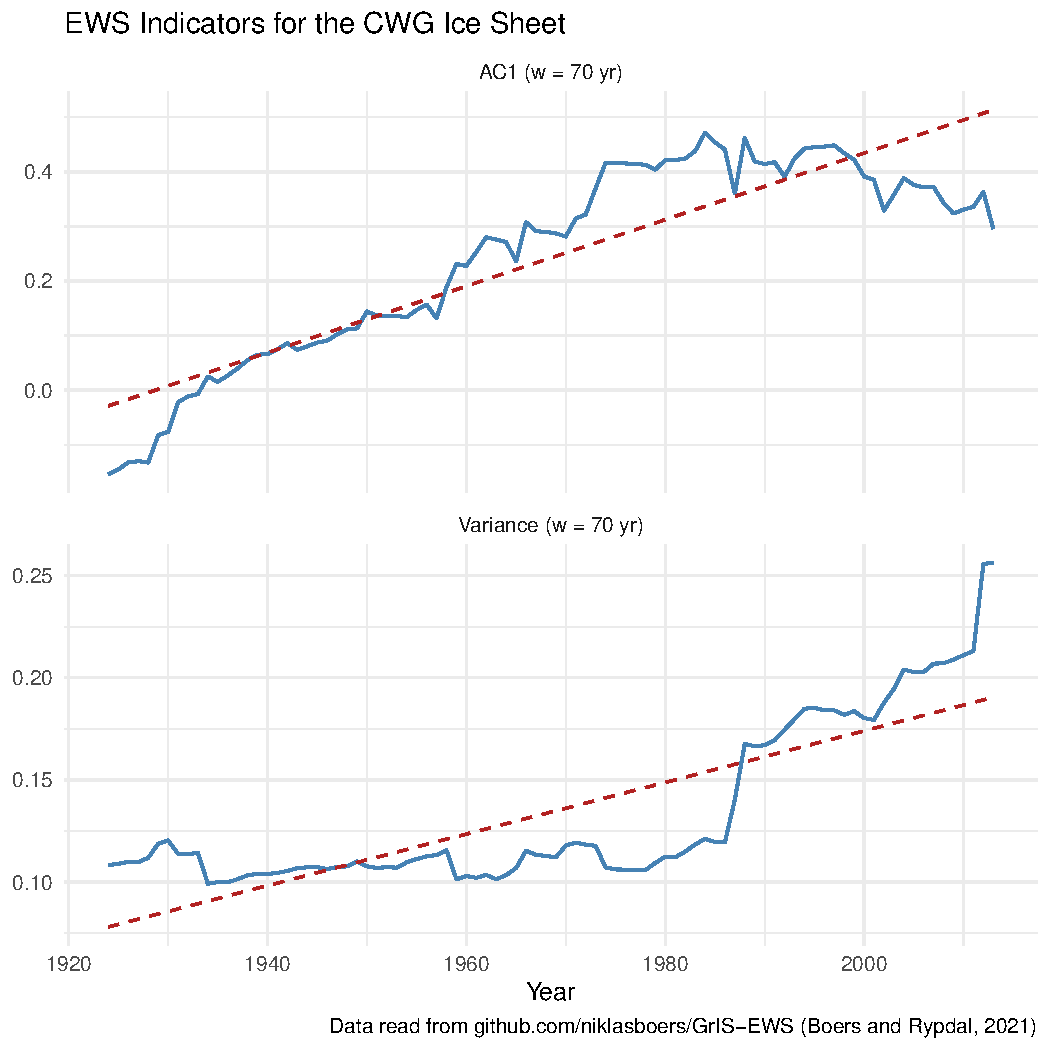
\includegraphics[width=0.85\linewidth]{work/09-tp-overview/figures/tp_ews_reproduction_plot} 

}

\caption{Reproduced variance and AC1 trends for the Central-Western Greenland melt record, following the method of Boers and Rypdal (2021).}\label{fig:tp-ews-plot}
\end{figure}

Figure \ref{fig:tp-ews-plot} shows both indicators over the analysis period.
OLS fits of the windowed series on year give a variance slope of
\(1.26\times10^{-3}\) yr\(^{-1}\) and an AC1 slope of
\(6.09\times10^{-3}\) yr\(^{-1}\) (90 window end years, from 1924 to 2013).
The associated regression \(t\)-tests yield \(p \ll 0.001\); given serial
dependence in the windowed series, these \(p\)-values are indicative.
Both indicators rise over the analysis period, in line with the pattern
reported by \citet{boers2021} (Fig. 1 D/E) for the same public melt record.

\section{Limitations of Early Warning Signals}\label{tp-limits}

EWS methods do not require a known threshold, but they have clear limits,
several of which \citet{rietkerk2025} emphasise.

\begin{itemize}
\item
  \textbf{Model dependence.} A clean rise in variance and AC1 toward a
  well-defined point is typical of simple, low-dimensional models. Complex
  Earth System Models, with many interacting feedbacks and strong spatial
  heterogeneity, need not show the same pattern even when a genuine tipping
  transition is under way.
\item
  \textbf{Ambiguous interpretation.} An EWS does not prove that a tipping point
  is approaching: other processes can raise autocorrelation and variance.
  Conversely, a tipping transition can occur without a detectable EWS,
  especially if it is noise-induced rather than driven by a slowly changing
  control parameter. An EWS is therefore neither necessary nor sufficient
  for an approaching tipping point.
\item
  \textbf{Statistical artefacts.} Sample variance can increase with record
  length even without a change in stability, and uncorrected spatial
  autocorrelation in gridded data can inflate apparent significance. Both
  effects invite overconfident claims about how close a system is to
  tipping.
\end{itemize}

In short, EWS are one strand of evidence. They are most useful when read
together with process understanding and physical modelling, as in the
Greenland case above, rather than as a stand-alone detection tool.

\section{Conclusion}\label{conclusion-3}

Tipping points matter because the transitions involved can be abrupt and
difficult to reverse. According to \citet{armstrongmckay2022}, several of the 16
tipping elements have estimated thresholds near 1.5--2°C above
pre-industrial levels. On that basis, a number of these elements may be
approached within the coming decades if warming continues along pathways
still considered in climate policy. Cascade interactions imply that some
transitions could occur earlier than thresholds estimated for isolated
systems would suggest. EWS based on critical slowing down provide one means
of monitoring stability without exact knowledge of the threshold. The
reproduction for Central-Western Greenland recovers the rising variance and
AC1 reported by \citet{boers2021} from the public melt record. At the same time,
the limitations discussed above indicate that EWS alone are not a reliable
predictor. Statistical monitoring therefore needs to be combined with
physically based models, and the issues raised by \citet{rietkerk2025} still need
to be addressed.

\section*{Use of AI Tools}\label{use-of-ai-tools}


I confirm that I completed this chapter independently and am fully
responsible for its content, including the R code.

I made limited use of \textbf{Cursor} (with a large language model) for:

\begin{itemize}
\tightlist
\item
  English editing of selected paragraphs;
\item
  structuring Section \ref{tp-thresholds} (splitting threshold estimation
  and sources of uncertainty);
\item
  technical help with R Markdown and the EWS reproduction scripts.
\end{itemize}

AI output was checked and revised by me. Scientific claims and numerical
results are based on the cited literature and my own code.

\chapter{Atlantic Meridional Overturning Circulation}\label{amoc}

\emph{Author: }

\emph{Supervisor: Helmut Küchenhoff}

\emph{Degree: Bachelor/Master}

\section{Abstract}\label{abstract-7}

Lorem ipsum dolor sit amet, consectetur adipiscing elit. Sed do eiusmod tempor incididunt ut labore et dolore magna aliqua. Ut enim ad minim veniam, quis nostrud exercitation ullamco laboris nisi ut aliquip ex ea commodo consequat. Duis aute irure dolor in reprehenderit in voluptate velit esse cillum dolore eu fugiat nulla pariatur. Excepteur sint occaecat cupidatat non proident, sunt in culpa qui officia deserunt mollit anim id est laborum.

\section{Introduction}\label{introduction-8}

\chapter{Positive tipping points}\label{ptp}

\emph{Author: Emir Arif Kilic}

\emph{Supervisor: Helmut Küchenhoff}

\emph{Degree: Master}

\section*{Abstract}\label{abstract-8}


Positive tipping points describe transitions where reinforcing feedbacks make desirable change increasingly self propelling. This chapter examines whether recent wind and solar trajectories in the three study countries show patterns consistent with such dynamics. Annual wind and solar generation shares from 2000 to 2025 are modelled using logistic S curves. Their fitted inflection years are then compared with changes in the fossil share.

Monthly fossil-share data is used to calculate rolling autocorrelation and variance. Denmark and the United Kingdom provide historical benchmark cases. These are examples of transitions that are already further advanced. Spain has an estimated inflection around 2021 while Germany reaches its fitted inflection near the end of the observed period. Poland has a projected inflection around 2029. The fossil share declines in all three countries although the early warning evidence is more mixed.

\section*{Introduction}\label{introduction-9}


Climate change mitigation requires a rapid transformation of energy systems. Cleaner electricity can reduce direct power sector emissions and support electrification in transport or heating. Energy systems are more than collections of technologies because firms and consumers influence how they develop. Infrastructure and policy also shape which options can expand.

It is easy to think of an electricity transition as a simple replacement of one technology by another. In reality firms make investment decisions under uncertainty and power plants remain in operation for many years. Electricity networks are also slow to change so existing infrastructure may continue to favour established technologies even when cleaner alternatives are available. Consumers may delay adoption when alternatives remain expensive or difficult to access. These conditions can slow the beginning of technological change \citep{lenton2023, geels2023}.

Transitions do not always continue at a constant speed. Greater deployment can reduce costs through learning and attract new investment. Users also become more familiar with a technology over time. Recent research uses national growth histories to study how wind and solar trajectories develop and differ \citep{jakhmola2026}.

\section*{Positive tipping points and feedback loops}\label{positive-tipping-points-and-feedback-loops}


A tipping point is the threshold beyond which change becomes self propelling and moves the system into a meaningfully different state. Before that threshold balancing feedbacks help preserve the existing state. Reinforcing feedbacks instead amplify change. A positive tipping point occurs when the reinforcing processes become strong enough to overcome the balancing ones \citep{lenton2026}.

A low carbon transition moves an existing system toward technologies and practices with lower emissions. Positive tipping may accelerate the spread of these alternatives. It may also weaken the established fossil fuel system which is referred to here as the incumbent system. The two processes can occur together \citep{lenton2026}.

One might think that rapid growth alone demonstrates a tipping point. However the central feature is that change improves the conditions for further change. Greater adoption may lower costs through learning by doing while better performance can increase demand. Infrastructure may expand as deployment grows and social acceptance can improve at the same time. These processes create reinforcing feedbacks that can make a transition increasingly self propelling \citep{lenton2026}.

Several mechanisms can contribute to this process. Social contagion means that adoption by some actors encourages others to adopt. Increasing returns arise when greater deployment lowers costs. Coordination matters when a technology becomes more useful as related infrastructure spreads. Percolation describes change through connected groups while co evolution links technological and institutional change \citep{lenton2026}.

A socio technical system combines technology with its surrounding actors and institutions. Geels and Ayoub describe seven interacting feedback loops linking technological development with firms or consumers. Policymakers and wider publics also shape the transition \citep{geels2023}.

\begin{table}

\caption{\label{tab:ptp-feedbackloops}Seven interacting socio technical feedback loops based on Geels and Ayoub.}
\centering
\begin{tabular}[t]{l|l}
\hline
Feedback loop & Reinforcing process\\
\hline
Users and technology & Adoption supports learning, lower costs and improved performance\\
\hline
Firms, technology and users & Demand encourages investment, production and technical development\\
\hline
Firms and policymakers & Growing industries gain influence and obtain stronger policy support\\
\hline
Policymakers, technology and users & Policy supports deployment and observed outcomes support policy learning\\
\hline
Users and wider publics & Adoption increases familiarity, visibility and social acceptance\\
\hline
Wider publics and technology & Technical improvement strengthens public legitimacy and support\\
\hline
Wider publics and policymakers & Public attention encourages policy action and shapes expectations\\
\hline
\end{tabular}
\end{table}

The loops can develop in different sequences. Technological deployment may occur before major changes in political commitment while another transition may begin with policy change. Public opinion can also shift before large technical changes become visible. Positive tipping is therefore better understood as a period of interacting developments than as one perfectly observable moment \citep{geels2023}.

\section*{Diffusion of innovation theory}\label{diffusion-of-innovation-theory}


Diffusion of innovation theory explains how a new technology spreads through a population or market. Adoption often begins with innovators and early adopters who accept more uncertainty and higher initial costs. Growth remains limited while the technology is unfamiliar or difficult to access. It accelerates when its advantages become easier to observe and a wider group becomes willing to adopt \citep{rogers2003}.

The cumulative adoption path often resembles an S curve. Its lower section represents early diffusion and the steep middle section shows rapid expansion. The upper section approaches saturation meaning the long run adoption level. The inflection point is where fitted growth is fastest.

National electricity generation shares do not directly measure the adopter groups described by Rogers. The theory instead motivates the aggregate diffusion pattern used here. Because cumulative diffusion is commonly represented by an S curve, the logistic models apply this structure to national wind and solar shares. They estimate the shape and timing of each country's aggregate diffusion path. FTT Power is an example of a more detailed model of power sector change that includes induced technological development \citep{mercure2012}.

\section*{Research questions}\label{research-questions}


RQ1. Do wind and solar generation shares in the three study countries follow S shaped diffusion paths and when do their fitted inflection points occur?

RQ2. How does the fossil share evolve relative to the fitted wind and solar inflection years?

RQ3. How do rolling autocorrelation and variance in monthly fossil-share residuals evolve relative to the fitted inflection years?

At first glance wind and solar growth may seem enough to describe the transition. However renewable generation could expand without reducing the fossil share if electricity demand also rises. The first question examines renewable diffusion and the second connects it with the incumbent system. The third considers whether short term fossil-share fluctuations change during the same period.

\section*{Benchmark transition cases}\label{benchmark-transition-cases}


Denmark and the United Kingdom are used as benchmark cases. Here a benchmark is an example that helps interpret less mature transitions rather than a formal control group. Denmark represents long renewable expansion while the United Kingdom shows rapid incumbent decline. The annual electricity data comes from Ember \citep{ember2026yearly}.

\begin{figure}

{\centering 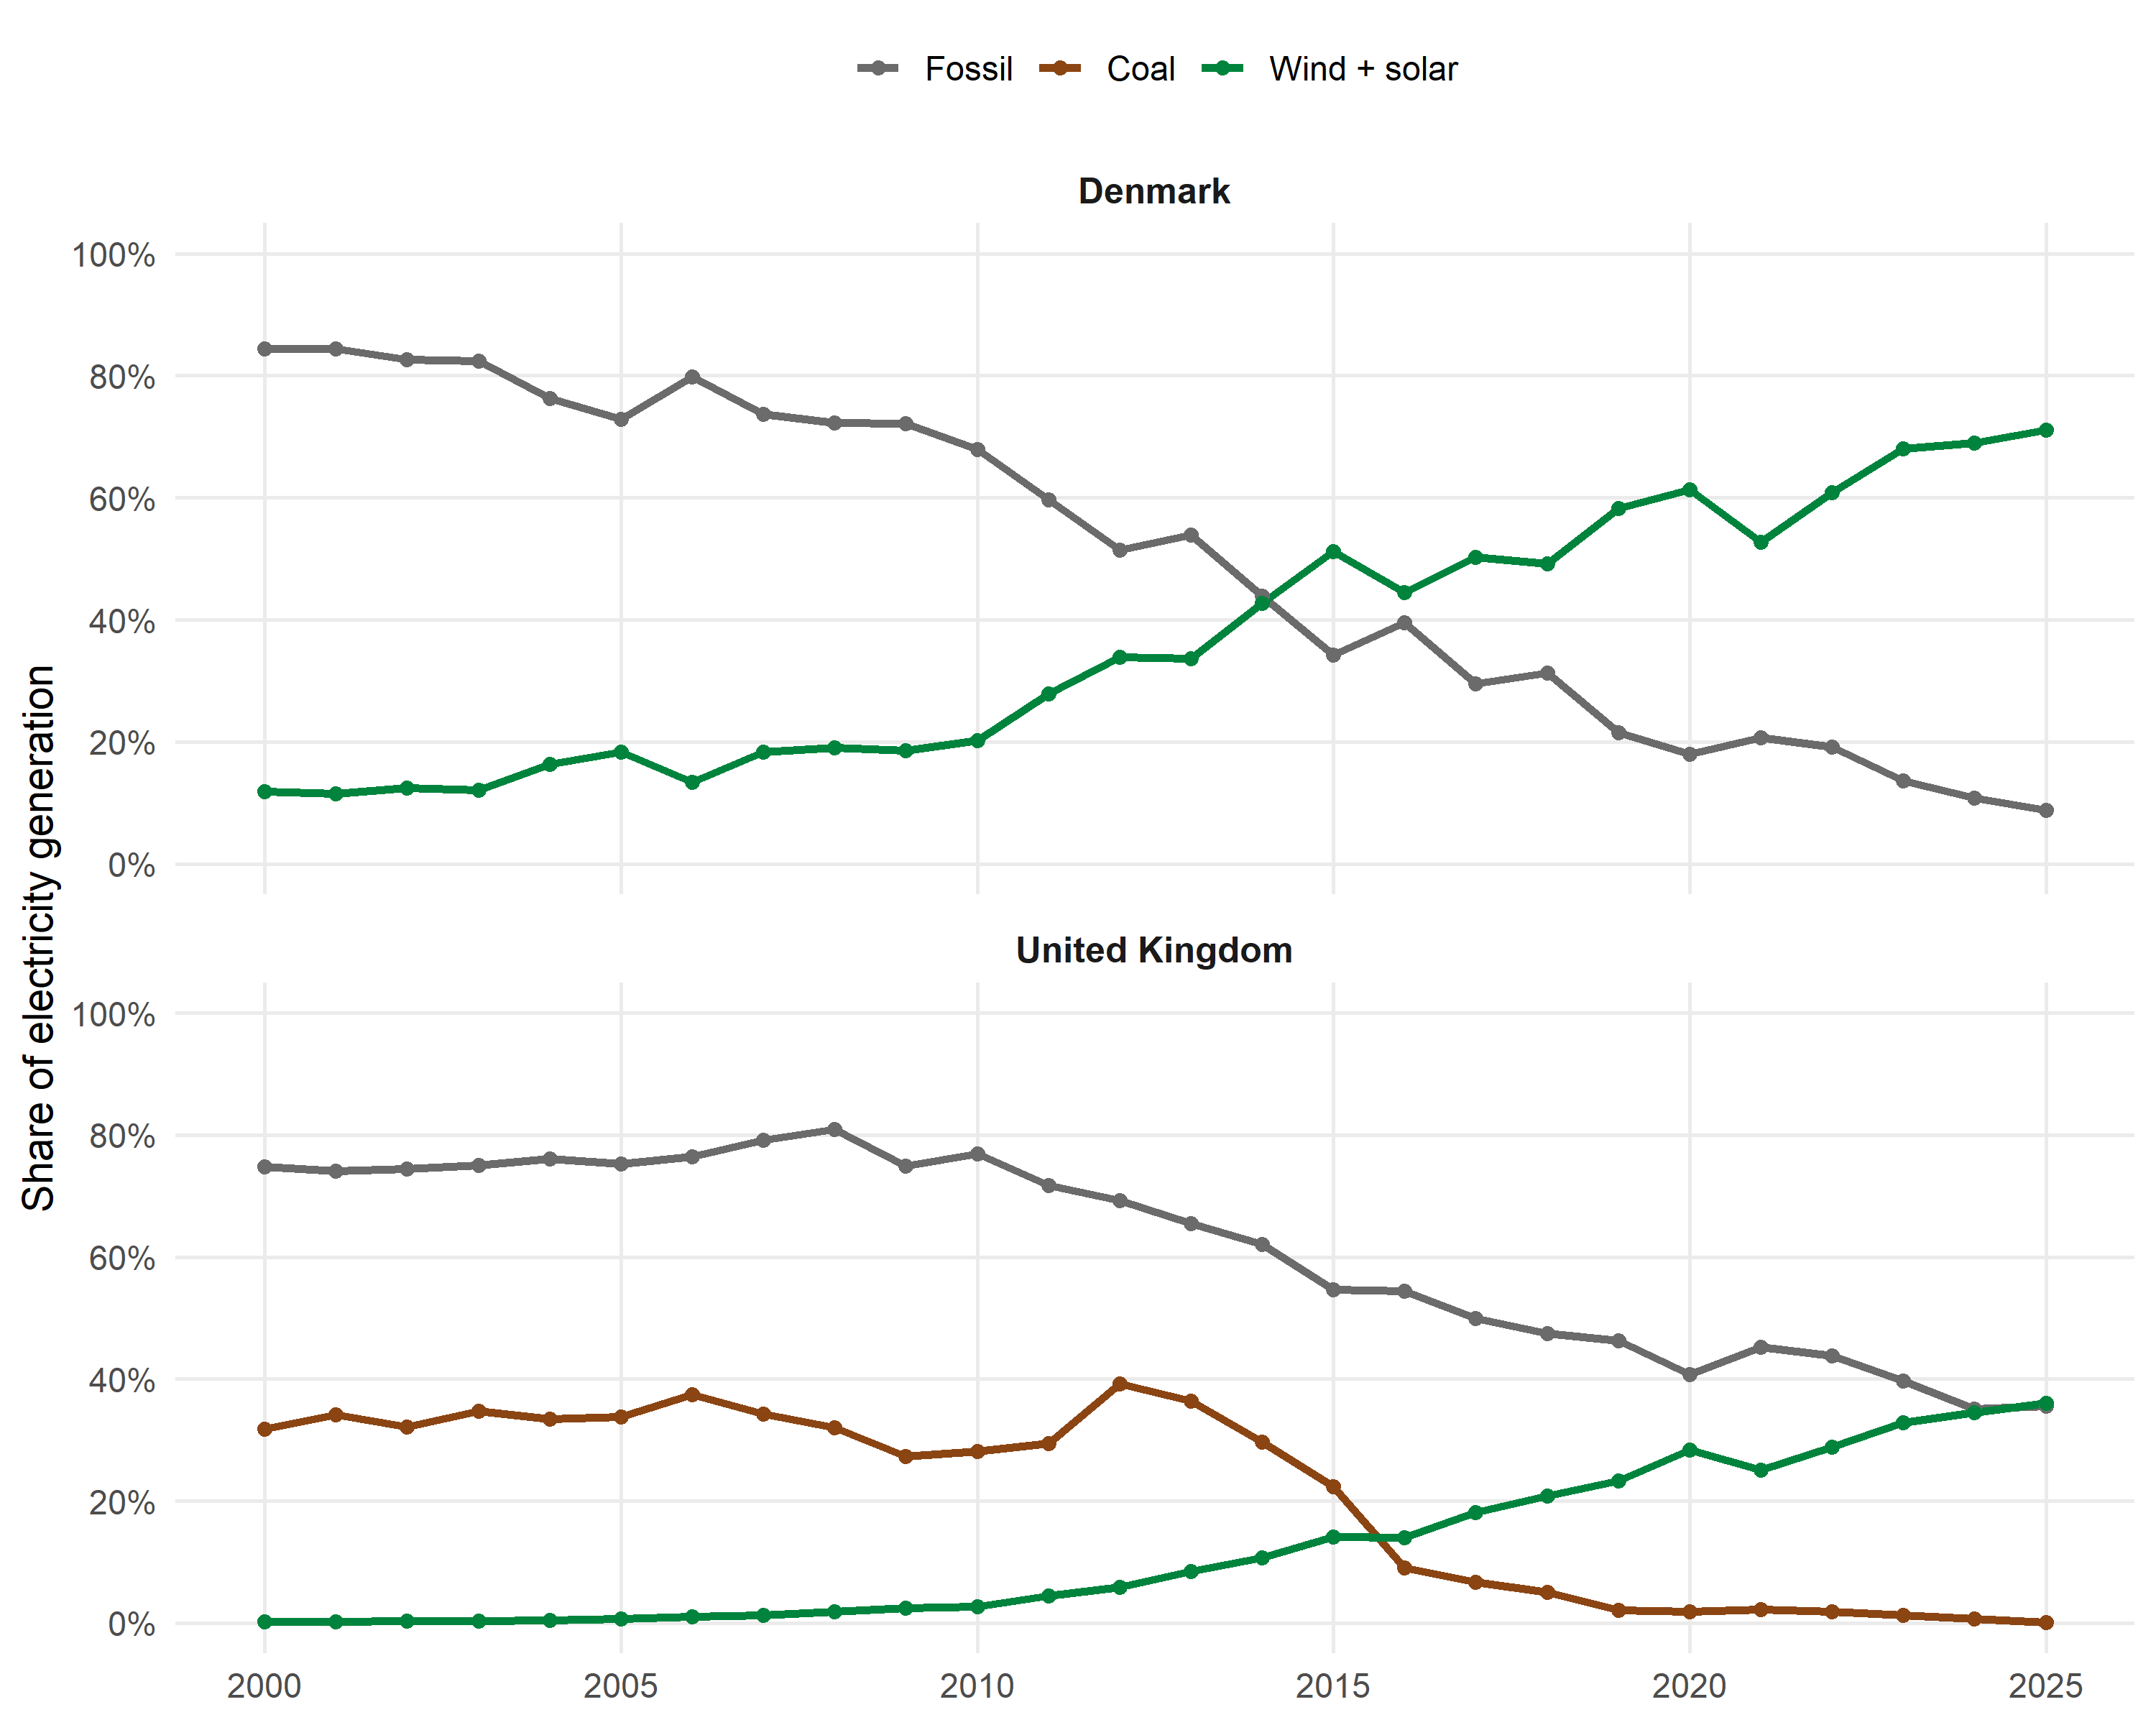
\includegraphics[width=0.9\linewidth]{work/11-positive_tp/figures/benchmark_context} 

}

\caption{Historical electricity transitions in Denmark and the United Kingdom. Coal is displayed separately for the United Kingdom.}\label{fig:ptp-benchmarkcontext}
\end{figure}

\subsection*{Denmark}\label{denmark}


Denmark's combined wind and solar share increased from around 12 percent in 2000 to more than 70 percent in 2025. The aggregate fossil share declined to around 10 percent. Growth was gradual during the early years and became stronger after 2010. Wind and solar later became the dominant part of the electricity mix. Denmark therefore represents a transition that has moved far beyond the early diffusion stage.

\subsection*{United Kingdom}\label{united-kingdom}


Wind and solar generation in the United Kingdom was close to zero in 2000 and increased rapidly after 2010. Coal is used separately for the British benchmark because the aggregate fossil category hides its unusually rapid disappearance. The clearest transition concerns coal which generated more than 30 percent of British electricity during much of the early sample. Its share declined rapidly after 2012 and reached almost zero by 2025. Carbon pricing weakened the economic position of coal and contributed to falling profitability. Plant closures then made a return to earlier coal generation levels less likely \citep{sharpe2021}.

\section*{Policy context}\label{policy-context}


The countries entered the transition with different policy ambitions.

\begin{longtable}[]{@{}
  >{\raggedright\arraybackslash}p{(\linewidth - 2\tabcolsep) * \real{0.5000}}
  >{\raggedright\arraybackslash}p{(\linewidth - 2\tabcolsep) * \real{0.5000}}@{}}
\caption{\label{tab:ptp-policycontext} Official 2030 electricity targets used as policy context.}\tabularnewline
\toprule\noalign{}
\begin{minipage}[b]{\linewidth}\raggedright
Country
\end{minipage} & \begin{minipage}[b]{\linewidth}\raggedright
Electricity target for 2030
\end{minipage} \\
\midrule\noalign{}
\endfirsthead
\toprule\noalign{}
\begin{minipage}[b]{\linewidth}\raggedright
Country
\end{minipage} & \begin{minipage}[b]{\linewidth}\raggedright
Electricity target for 2030
\end{minipage} \\
\midrule\noalign{}
\endhead
\bottomrule\noalign{}
\endlastfoot
Denmark & Renewable output covering 100 percent of electricity demand \citep{denmark2026} \\
United Kingdom & At least 95 percent clean generation \citep{govuk2024} \\
Spain & 81 percent renewable generation \citep{miteco2024} \\
Germany & 80 percent of gross electricity consumption from renewables \citep{bmwk2026} \\
Poland & At least 32 percent renewable electricity under the 2020 NECP \citep{europeancommission2020} \\
\end{longtable}

\section*{Data and country context}\label{data-and-country-context}


The analysis uses yearly and monthly electricity data from Ember \citep{ember2026yearly, ember2026monthly}. The yearly dataset covers 2000 to 2025 and the main variable is the combined wind and solar share of national electricity generation. Aggregate fossil shares describe the incumbent electricity system.

The monthly dataset covers January 2015 to December 2025 and contains aggregate fossil shares for Spain, Germany and Poland. These observations are used to construct the monthly residual series for the early warning analysis.

\begin{figure}

{\centering 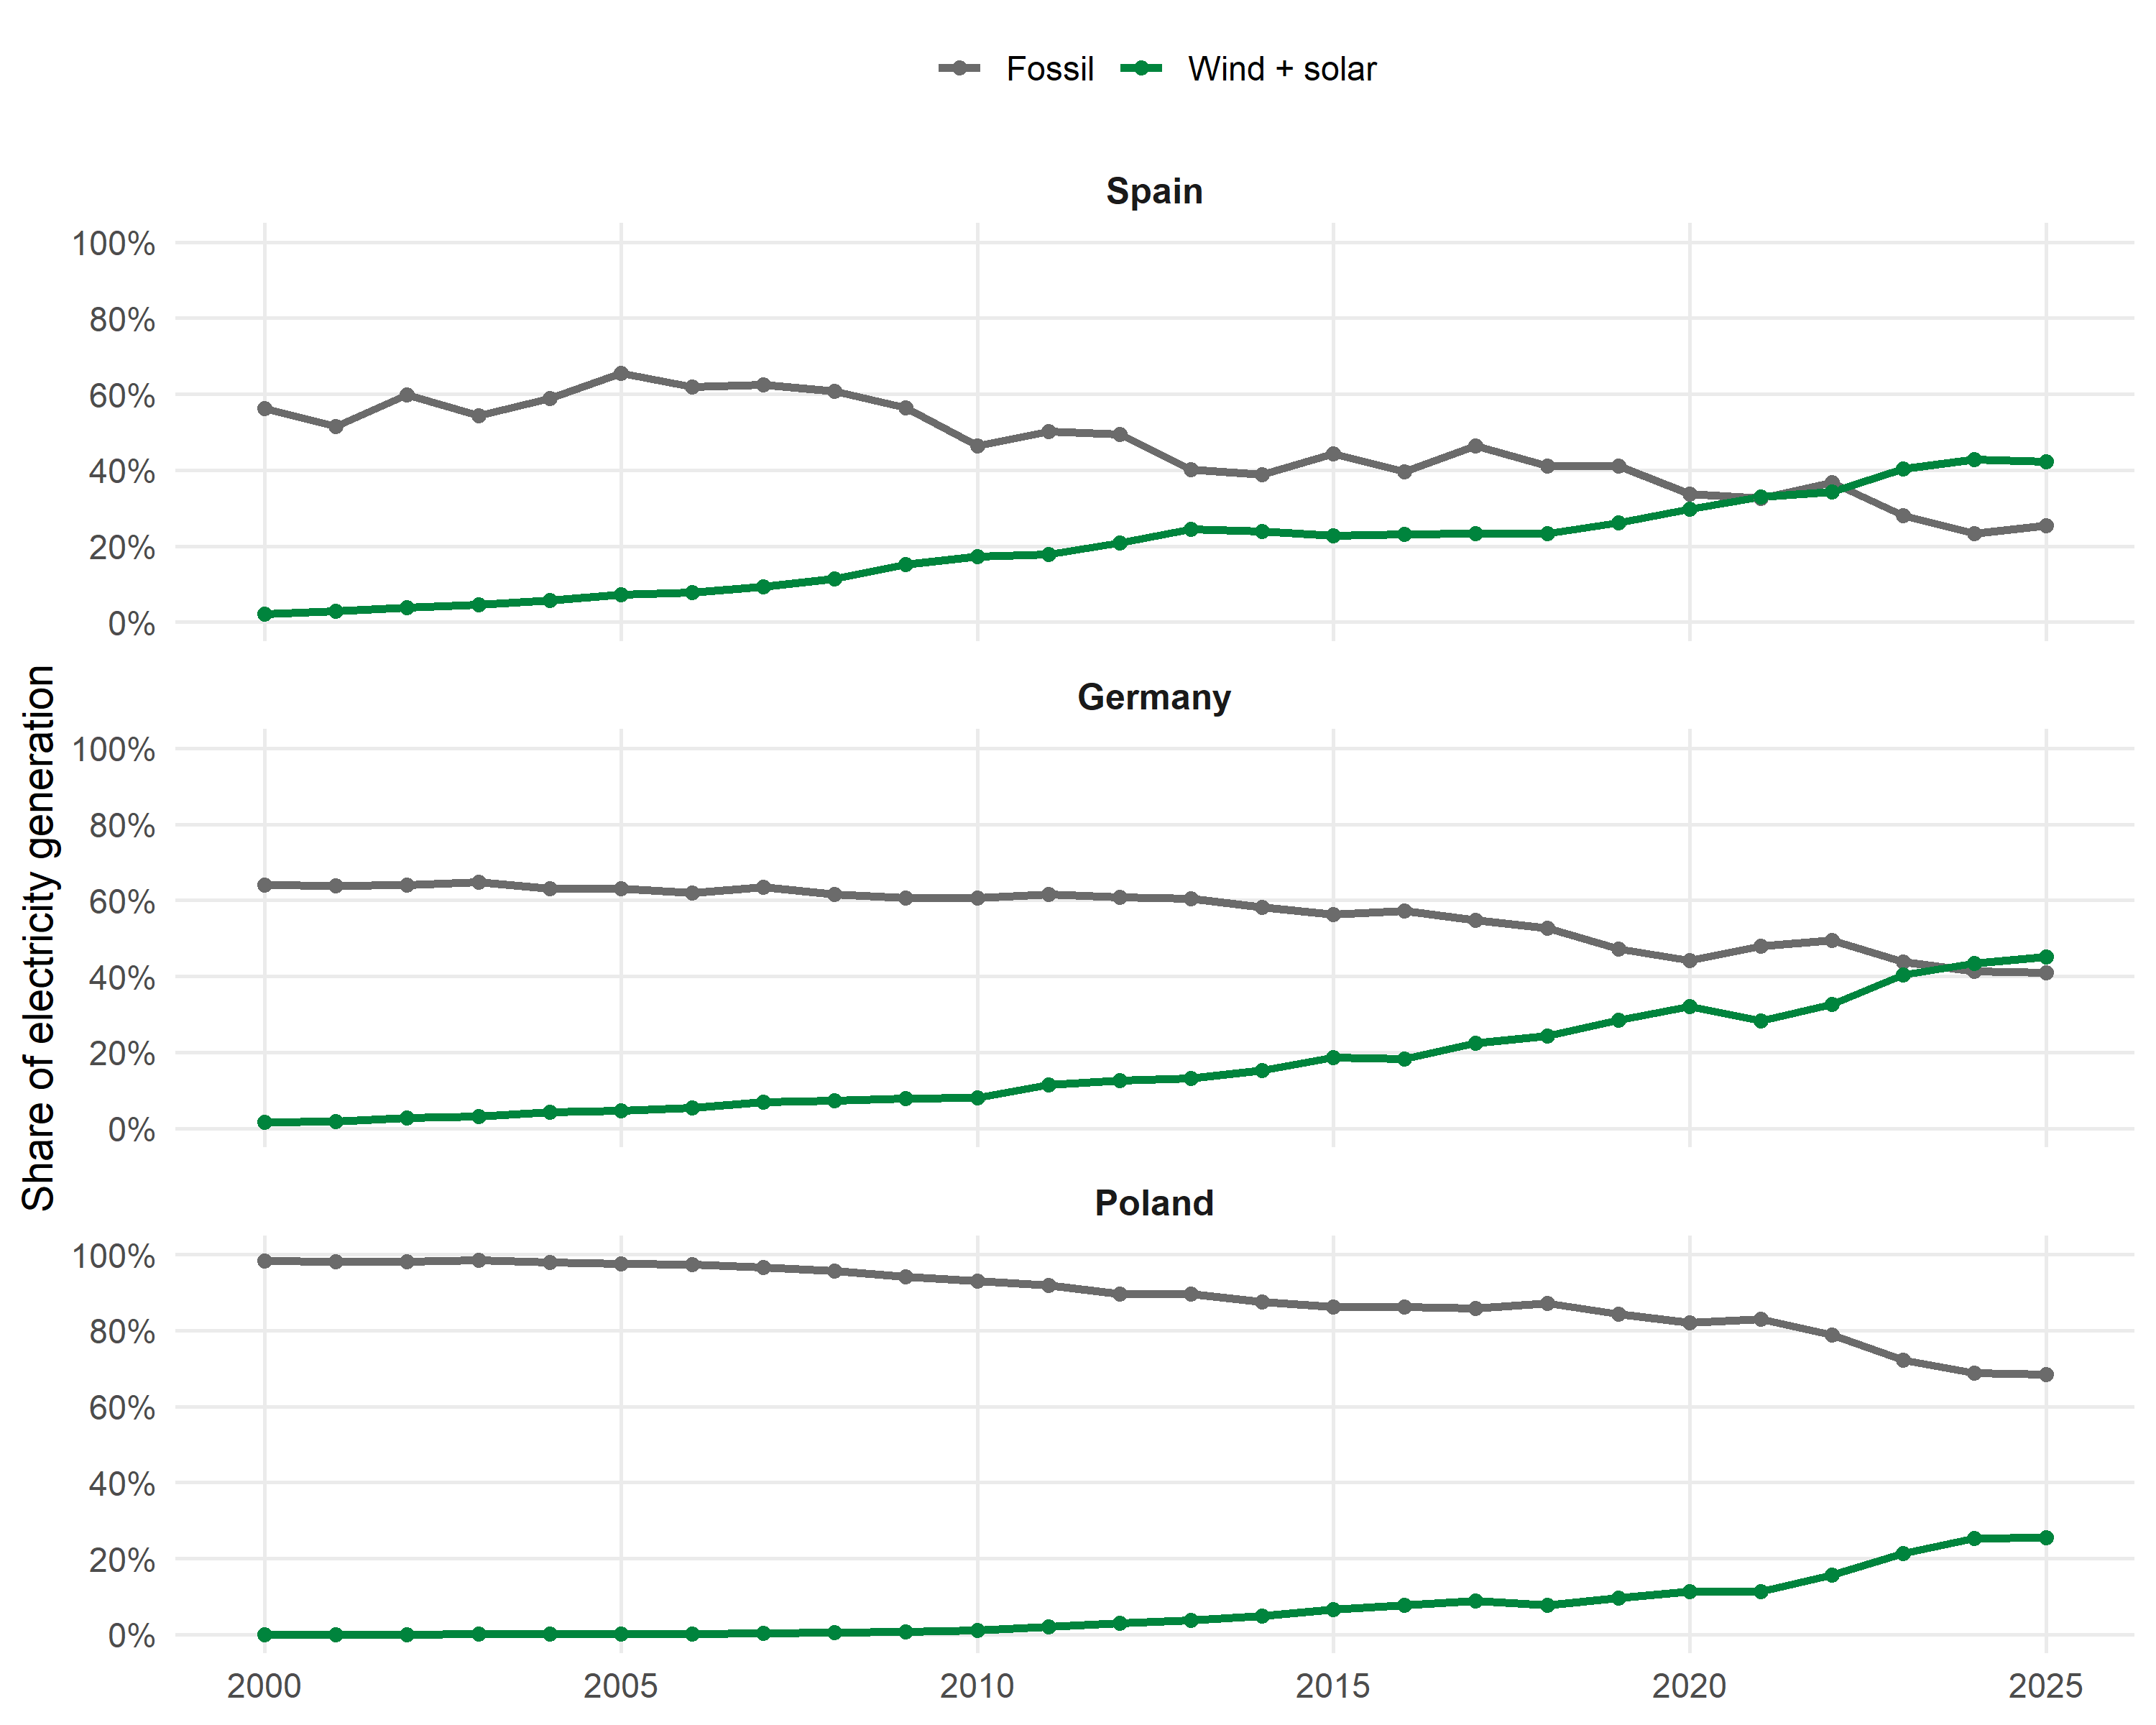
\includegraphics[width=0.9\linewidth]{work/11-positive_tp/figures/country_context} 

}

\caption{Annual fossil and wind and solar shares of electricity generation in Spain, Germany and Poland from 2000 to 2025.}\label{fig:ptp-maincontext}
\end{figure}

Spain shows the earliest convergence and the wind and solar share exceeds the fossil share near the end of the sample. Germany also approaches parity. Poland experiences rapid recent renewable growth although the fossil share remains dominant.

\section*{Statistical methods}\label{statistical-methods}


\subsection*{Logistic diffusion model}\label{logistic-diffusion-model}


The wind and solar share is represented using a logistic curve for each country.

\[
y_t =
\frac{K}
{1+e^{-r(t-t_0)}}
+\varepsilon_t.
\]

Here \(y_t\) is the wind and solar share in year \(t\). The parameter \(K\) is the saturation level and \(r\) controls the diffusion speed. The parameter \(t_0\) is the inflection year while \(\varepsilon_t\) is the difference between the observed and fitted value. At the inflection point the fitted share equals half of the saturation level.

\[
\hat{y}_{t_0}=\frac{K}{2}.
\]

The fitted trajectory grows most rapidly around \(t_0\). Parameter estimates in macro level diffusion models can change systematically as observations are added \citep{vandenbulte1997}. The model is therefore fitted over a grid of fixed saturation levels which limits instability when only part of the diffusion path is observed.

The candidate values for \(K\) begin one integer above the rounded-up observed maximum for each country and are capped at 90 percent. The preferred value of \(K\) is selected using the historical root mean squared error abbreviated as RMSE. RMSE measures the typical distance between the observed share and the fitted curve.

\[
RMSE =
\sqrt{
\frac{1}{n}
\sum_{t=1}^{n}
(y_t-\hat{y}_t)^2
}.
\]

Here \(n\) is the number of annual observations and \(\hat{y}_t\) is the fitted share. Alternative curves use saturation levels of 50 percent and 70 percent with an 80 percent curve included as well. They show how the assumed long run limit affects the projection.

\subsection*{Bootstrap bands}\label{bootstrap-bands}


A residual bootstrap represents uncertainty around the selected curve. A residual is the observed value minus the fitted value. Residuals are sampled with replacement and added to the curve. For each bootstrap sample, \(r\) and \(t_0\) are re-estimated while the selected saturation level \(K\) remains fixed. The procedure produces 200 projected paths through 2035 whose 2.5th and 97.5th percentiles form the displayed band.

\subsection*{Fossil displacement}\label{fossil-displacement}


Fossil displacement refers here to a decline in the fossil share while the wind and solar share expands. The fitted renewable inflection years are placed on national fossil-share plots. This allows the timing of renewable acceleration to be compared with the development of the incumbent electricity system. A decline around the estimated inflection provides additional descriptive evidence of wider system change.

\subsection*{Early warning indicators}\label{early-warning-indicators}


A critical transition is a large shift between system states. Systems approaching one may recover more slowly from disturbances, a process called critical slowing down. Greater persistence may appear as rising lag one autocorrelation while larger fluctuations may appear as rising variance \citep{scheffer2009}. Autocorrelation relates current and earlier residuals whereas variance measures their spread.

A simple autoregressive process can be written as

\[
x_t =
\alpha x_{t-1}
+\varepsilon_t.
\]

Here \(x_t\) is the current monthly fossil-share residual and \(x_{t-1}\) is the residual from the previous month. The parameter \(\alpha\) measures how strongly the previous disturbance remains in the system, while \(\varepsilon_t\) represents the new disturbance occurring in month \(t\). Because the data are monthly lag one corresponds to a one month gap.

\[
AR(1)=
\operatorname{corr}(x_t,x_{t-1}).
\]

The variance is

\[
\operatorname{Var}(x)=
\frac{1}{n-1}
\sum_{t=1}^{n}
(x_t-\bar{x})^2.
\]

Here \(n\) is the number of months in the rolling window and \(\bar{x}\) is the mean residual within that window. Because the residuals are measured in percentage points, variance is measured in squared percentage points.

Monthly fossil shares are separated into seasonal, trend and residual components using robust seasonal trend decomposition. The residual contains the short term fluctuations left after seasonality and trend are removed. AR(1) and variance are estimated within rolling windows of 36 months. Similar indicators have been applied to technological transitions to examine whether an incumbent technology is losing stability \citep{mercure2026}.

\section*{Results}\label{results-5}


\subsection*{Wind and solar diffusion}\label{wind-and-solar-diffusion}


\begin{table}

\caption{\label{tab:ptp-selectedmodels}Selected logistic S curve parameters based on historical RMSE.}
\centering
\begin{tabular}[t]{l|r|r|r|r}
\hline
Country & Saturation K & Diffusion rate r & Inflection year t0 & RMSE\\
\hline
Spain & 67 & 0.123 & 2021 & 2.618\\
\hline
Germany & 88 & 0.146 & 2025 & 1.380\\
\hline
Poland & 90 & 0.200 & 2029 & 1.160\\
\hline
\end{tabular}
\end{table}

Spain has a selected saturation level of 67 percent. Its estimated diffusion rate is 0.123 and the fitted inflection occurs around 2020.8. The RMSE is 2.62 percentage points. Germany has a selected saturation level of 88 percent and an estimated diffusion rate of 0.146. Its fitted inflection occurs around 2024.6 with an RMSE of 1.38 percentage points.

Poland has the fastest estimated diffusion rate at 0.200. Its fitted inflection occurs around 2029.3 and the selected saturation level reaches the imposed maximum of 90 percent. This upper boundary becomes important when interpreting the later part of the Polish projection.

\subsection*{Spain}\label{spain}


\begin{figure}

{\centering 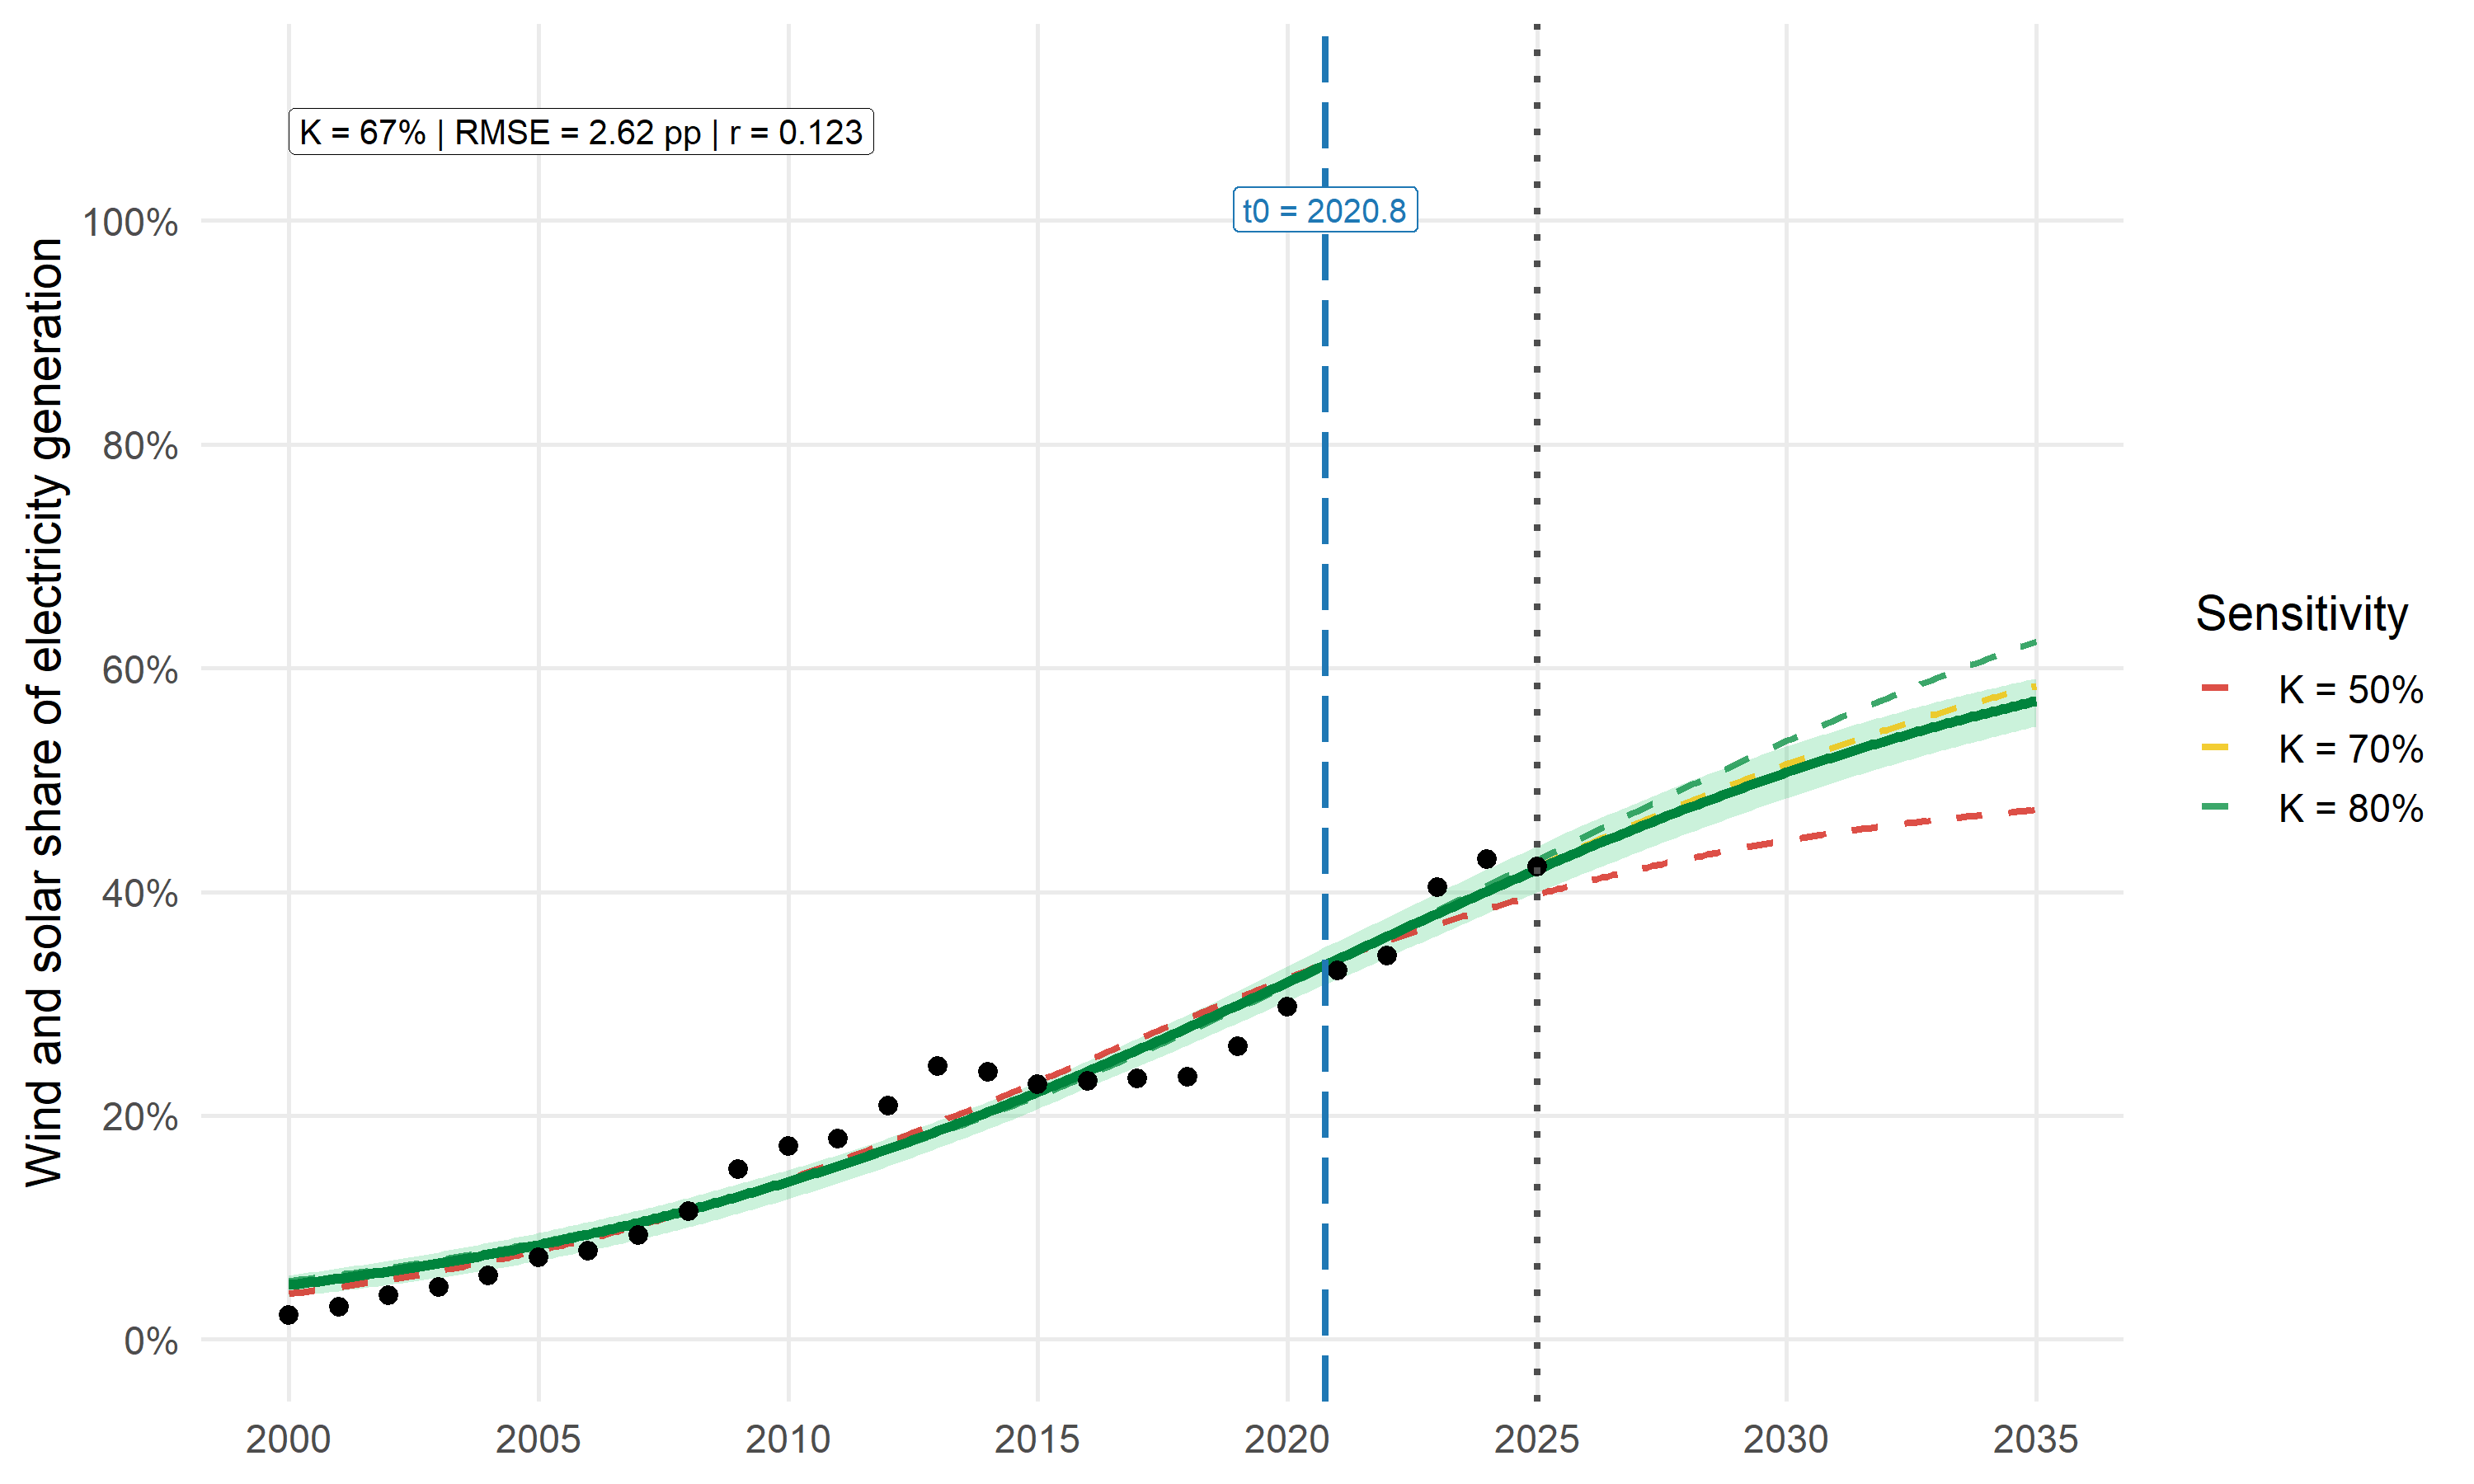
\includegraphics[width=0.9\linewidth]{work/11-positive_tp/figures/spain_scurve} 

}

\caption{Observed and fitted wind and solar electricity shares in Spain. The shaded area is the residual bootstrap band. Dashed curves use alternative saturation assumptions.}\label{fig:ptp-spainscurve}
\end{figure}

Spain shows gradual early growth followed by stronger expansion after 2010. The selected model estimates the inflection around 2020.8, which lies within the observed period, so Spain represents an observed inflection case. Similar historical fits can therefore produce different long run projections.

\subsection*{Germany}\label{germany}


\begin{figure}

{\centering 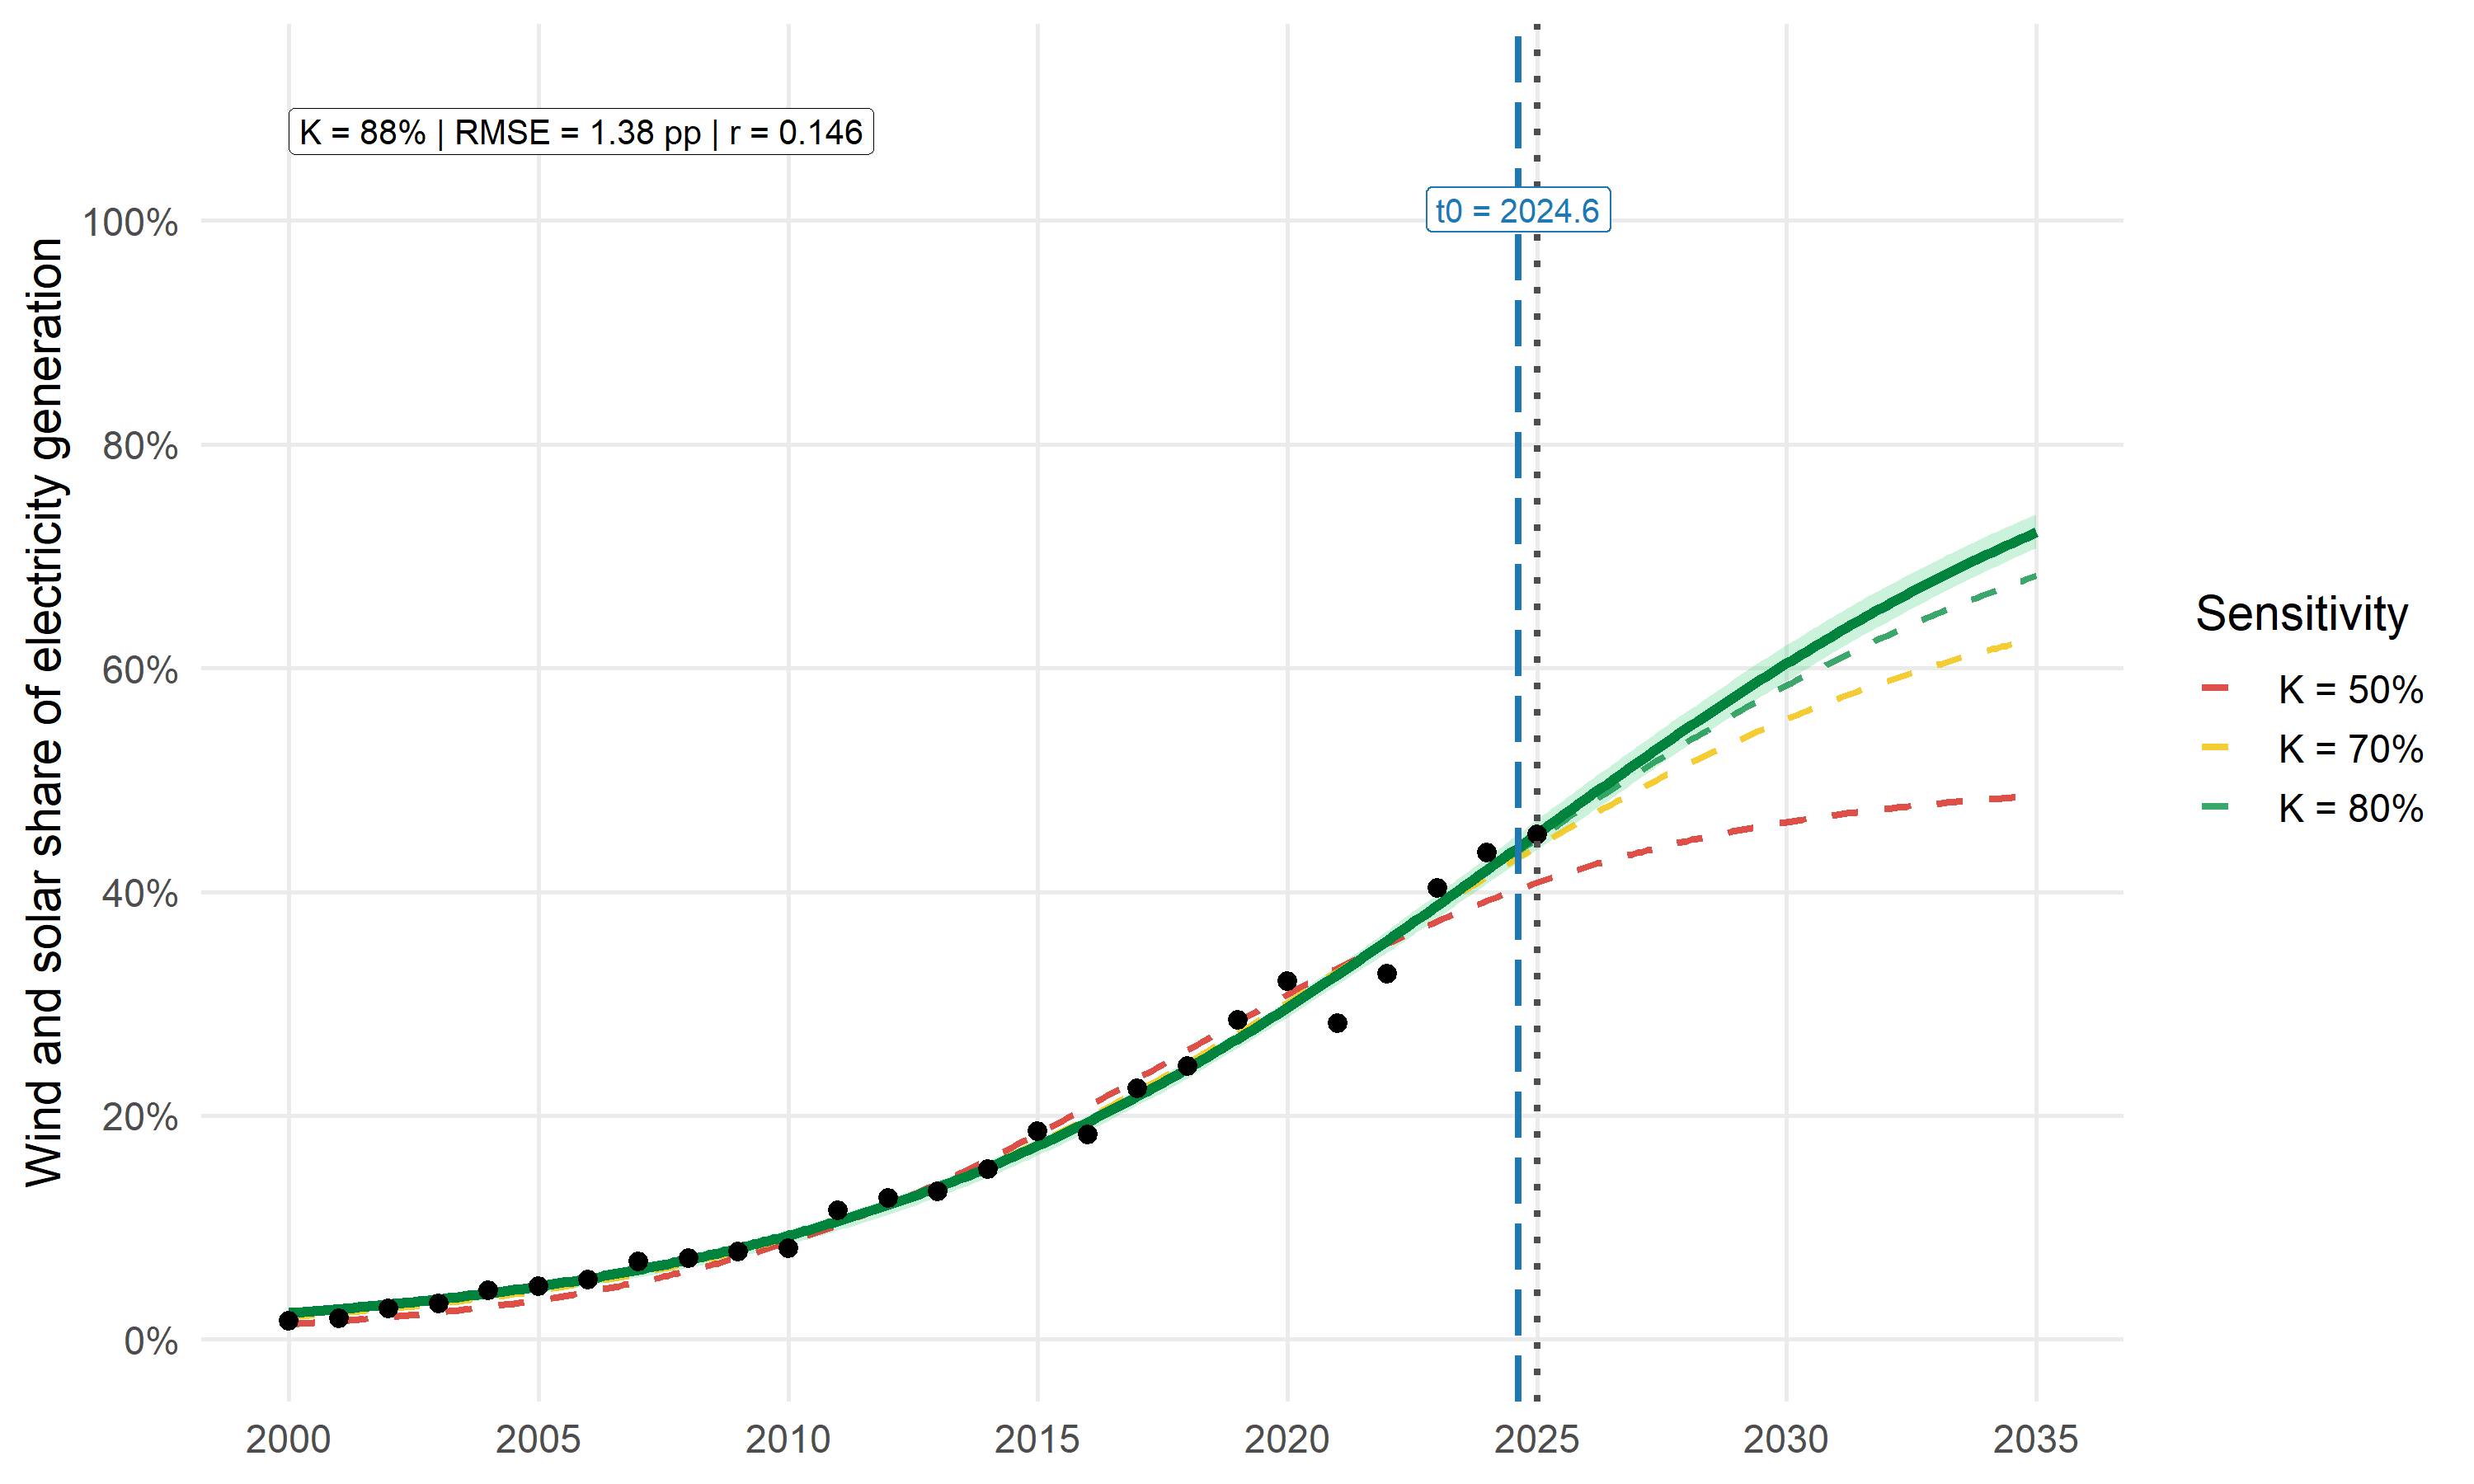
\includegraphics[width=0.9\linewidth]{work/11-positive_tp/figures/germany_scurve} 

}

\caption{Observed and fitted wind and solar electricity shares in Germany. The fitted inflection occurs near the end of the observed period.}\label{fig:ptp-germanyscurve}
\end{figure}

Germany follows the selected logistic trajectory closely. The estimated inflection year is 2024.6 and lies near the final observed year. Germany therefore represents a near term inflection case although only a short part of the trajectory after the fitted inflection is observed.

\subsection*{Poland}\label{poland}


\begin{figure}

{\centering 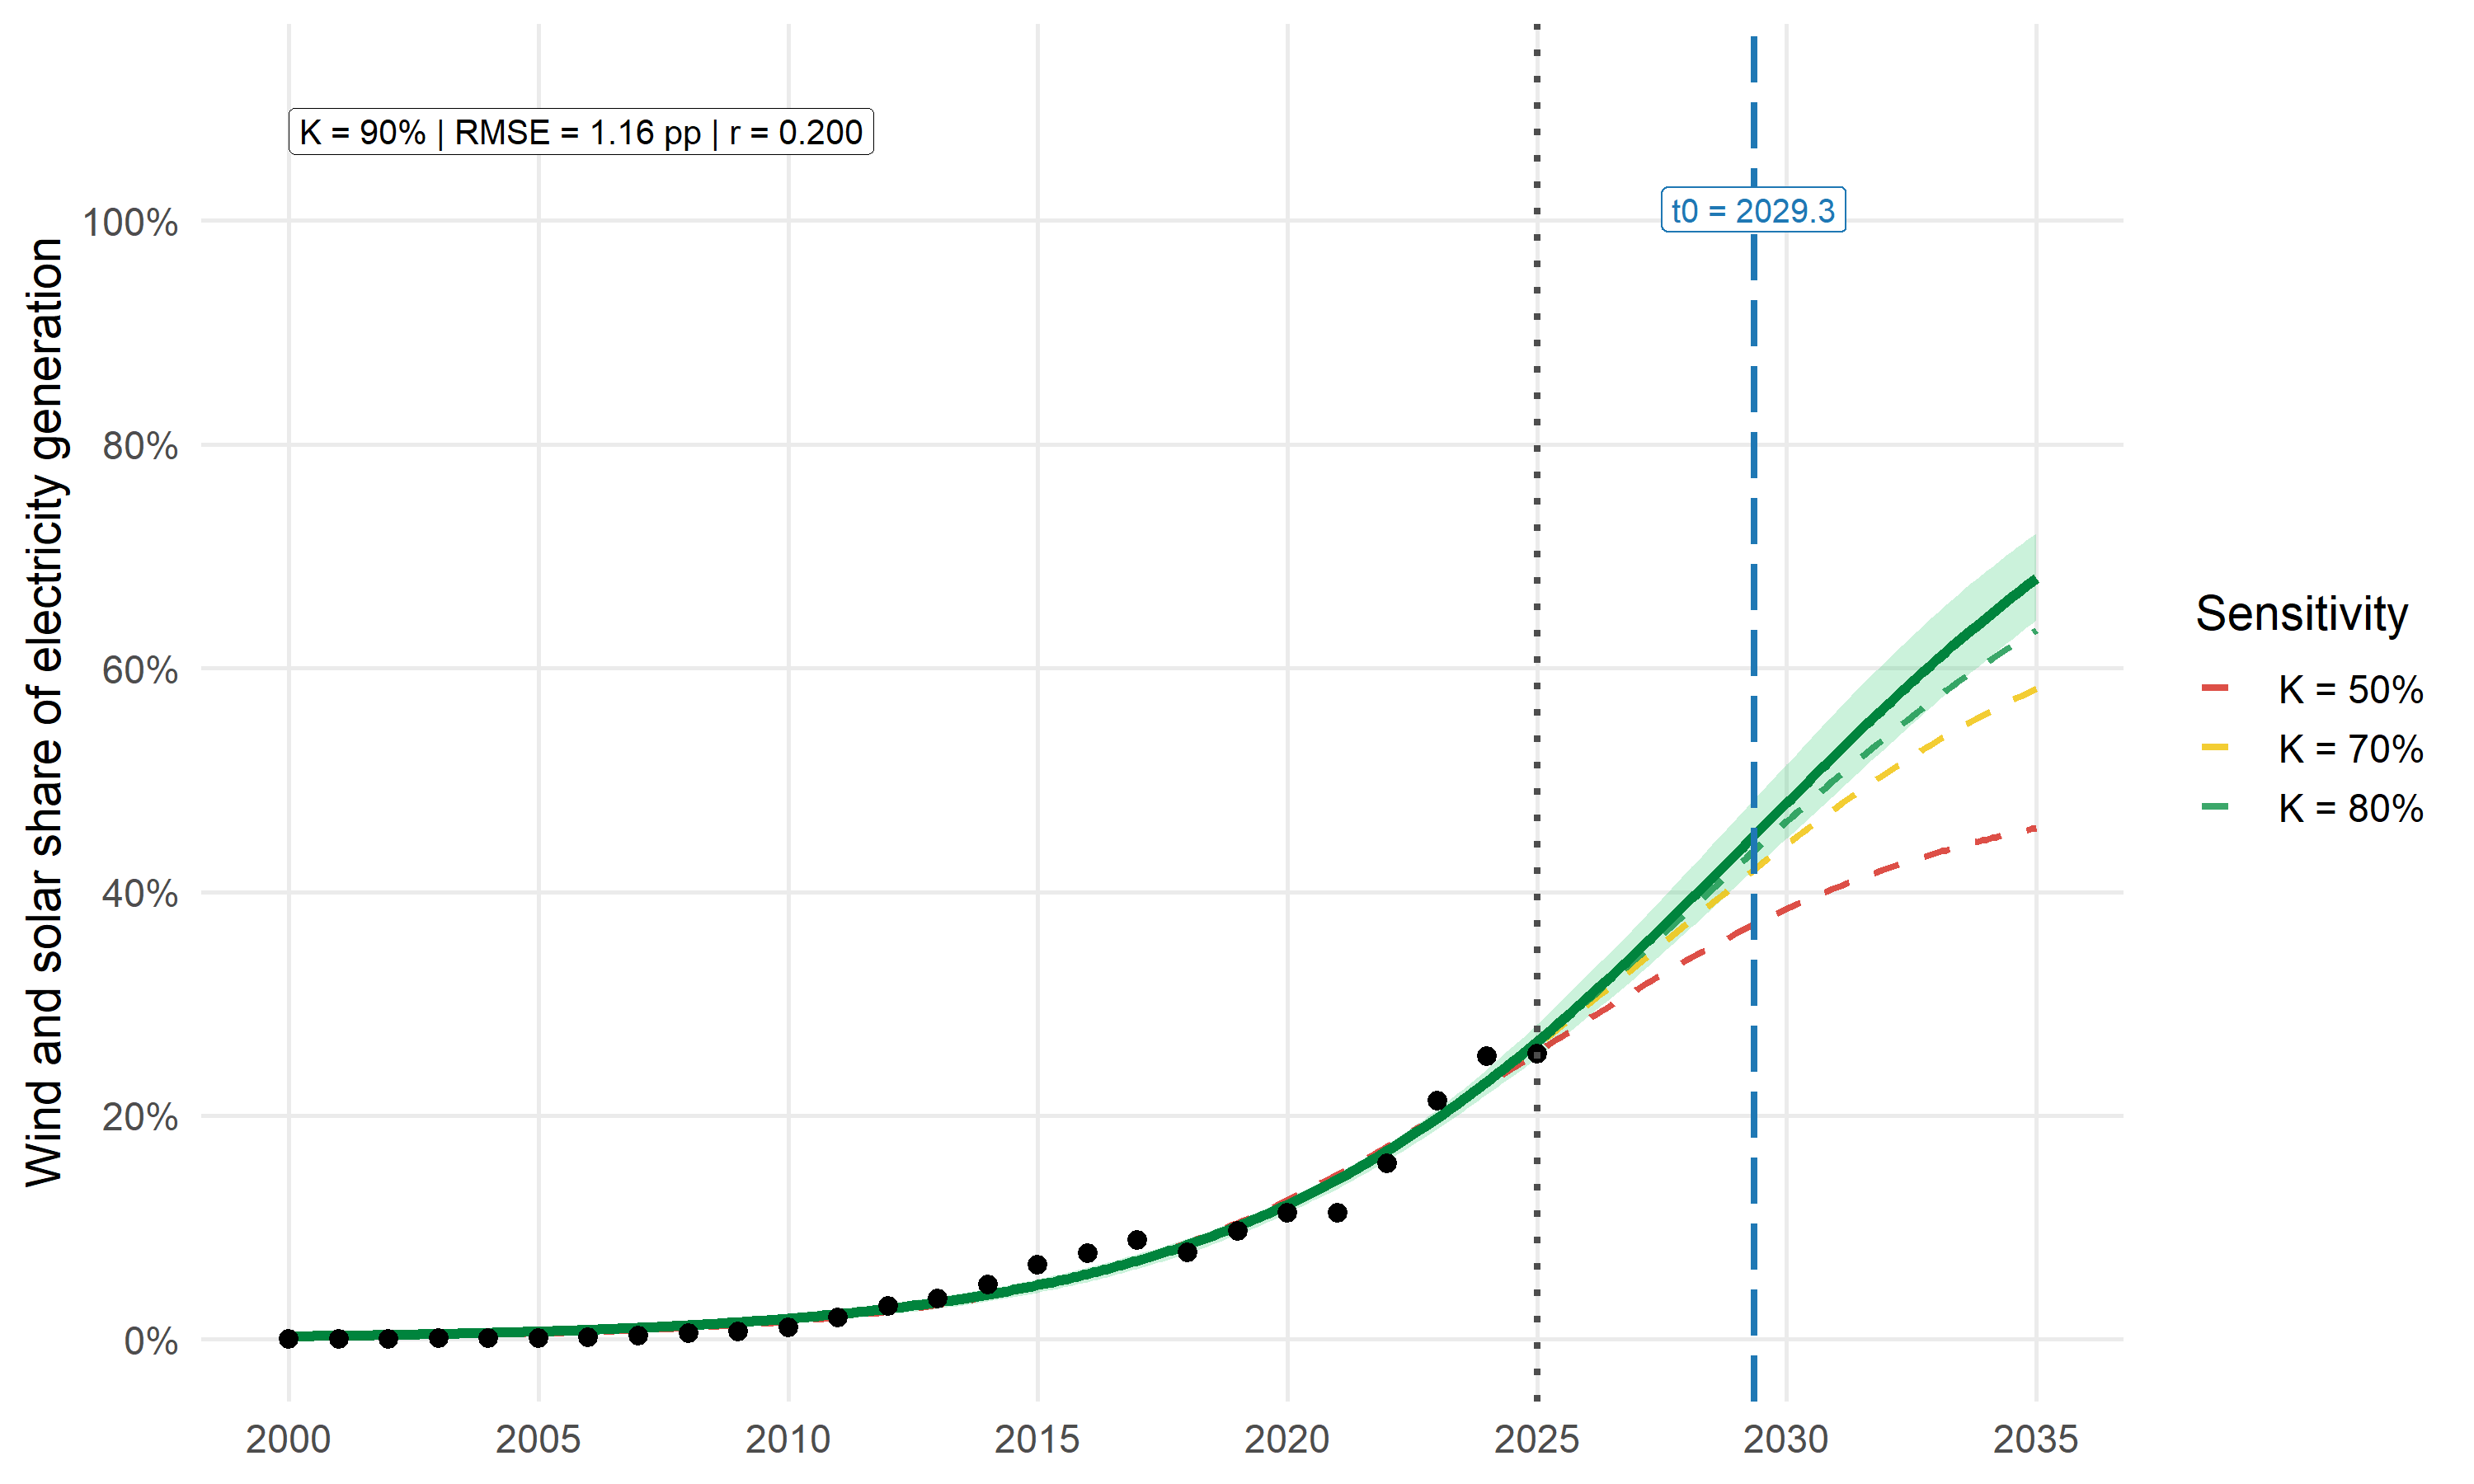
\includegraphics[width=0.9\linewidth]{work/11-positive_tp/figures/poland_scurve} 

}

\caption{Observed and fitted wind and solar electricity shares in Poland. The fitted inflection occurs after the observed period.}\label{fig:ptp-polandscurve}
\end{figure}

Poland begins with almost no wind and solar generation. Growth becomes visible after 2010 and accelerates after 2020. The projected inflection around 2029 lies outside the observed period. Its selected saturation level also reaches the maximum considered value so the later projection is especially sensitive to the assumed upper limit.

\subsection*{Fossil displacement}\label{fossil-displacement-1}


\begin{figure}

{\centering 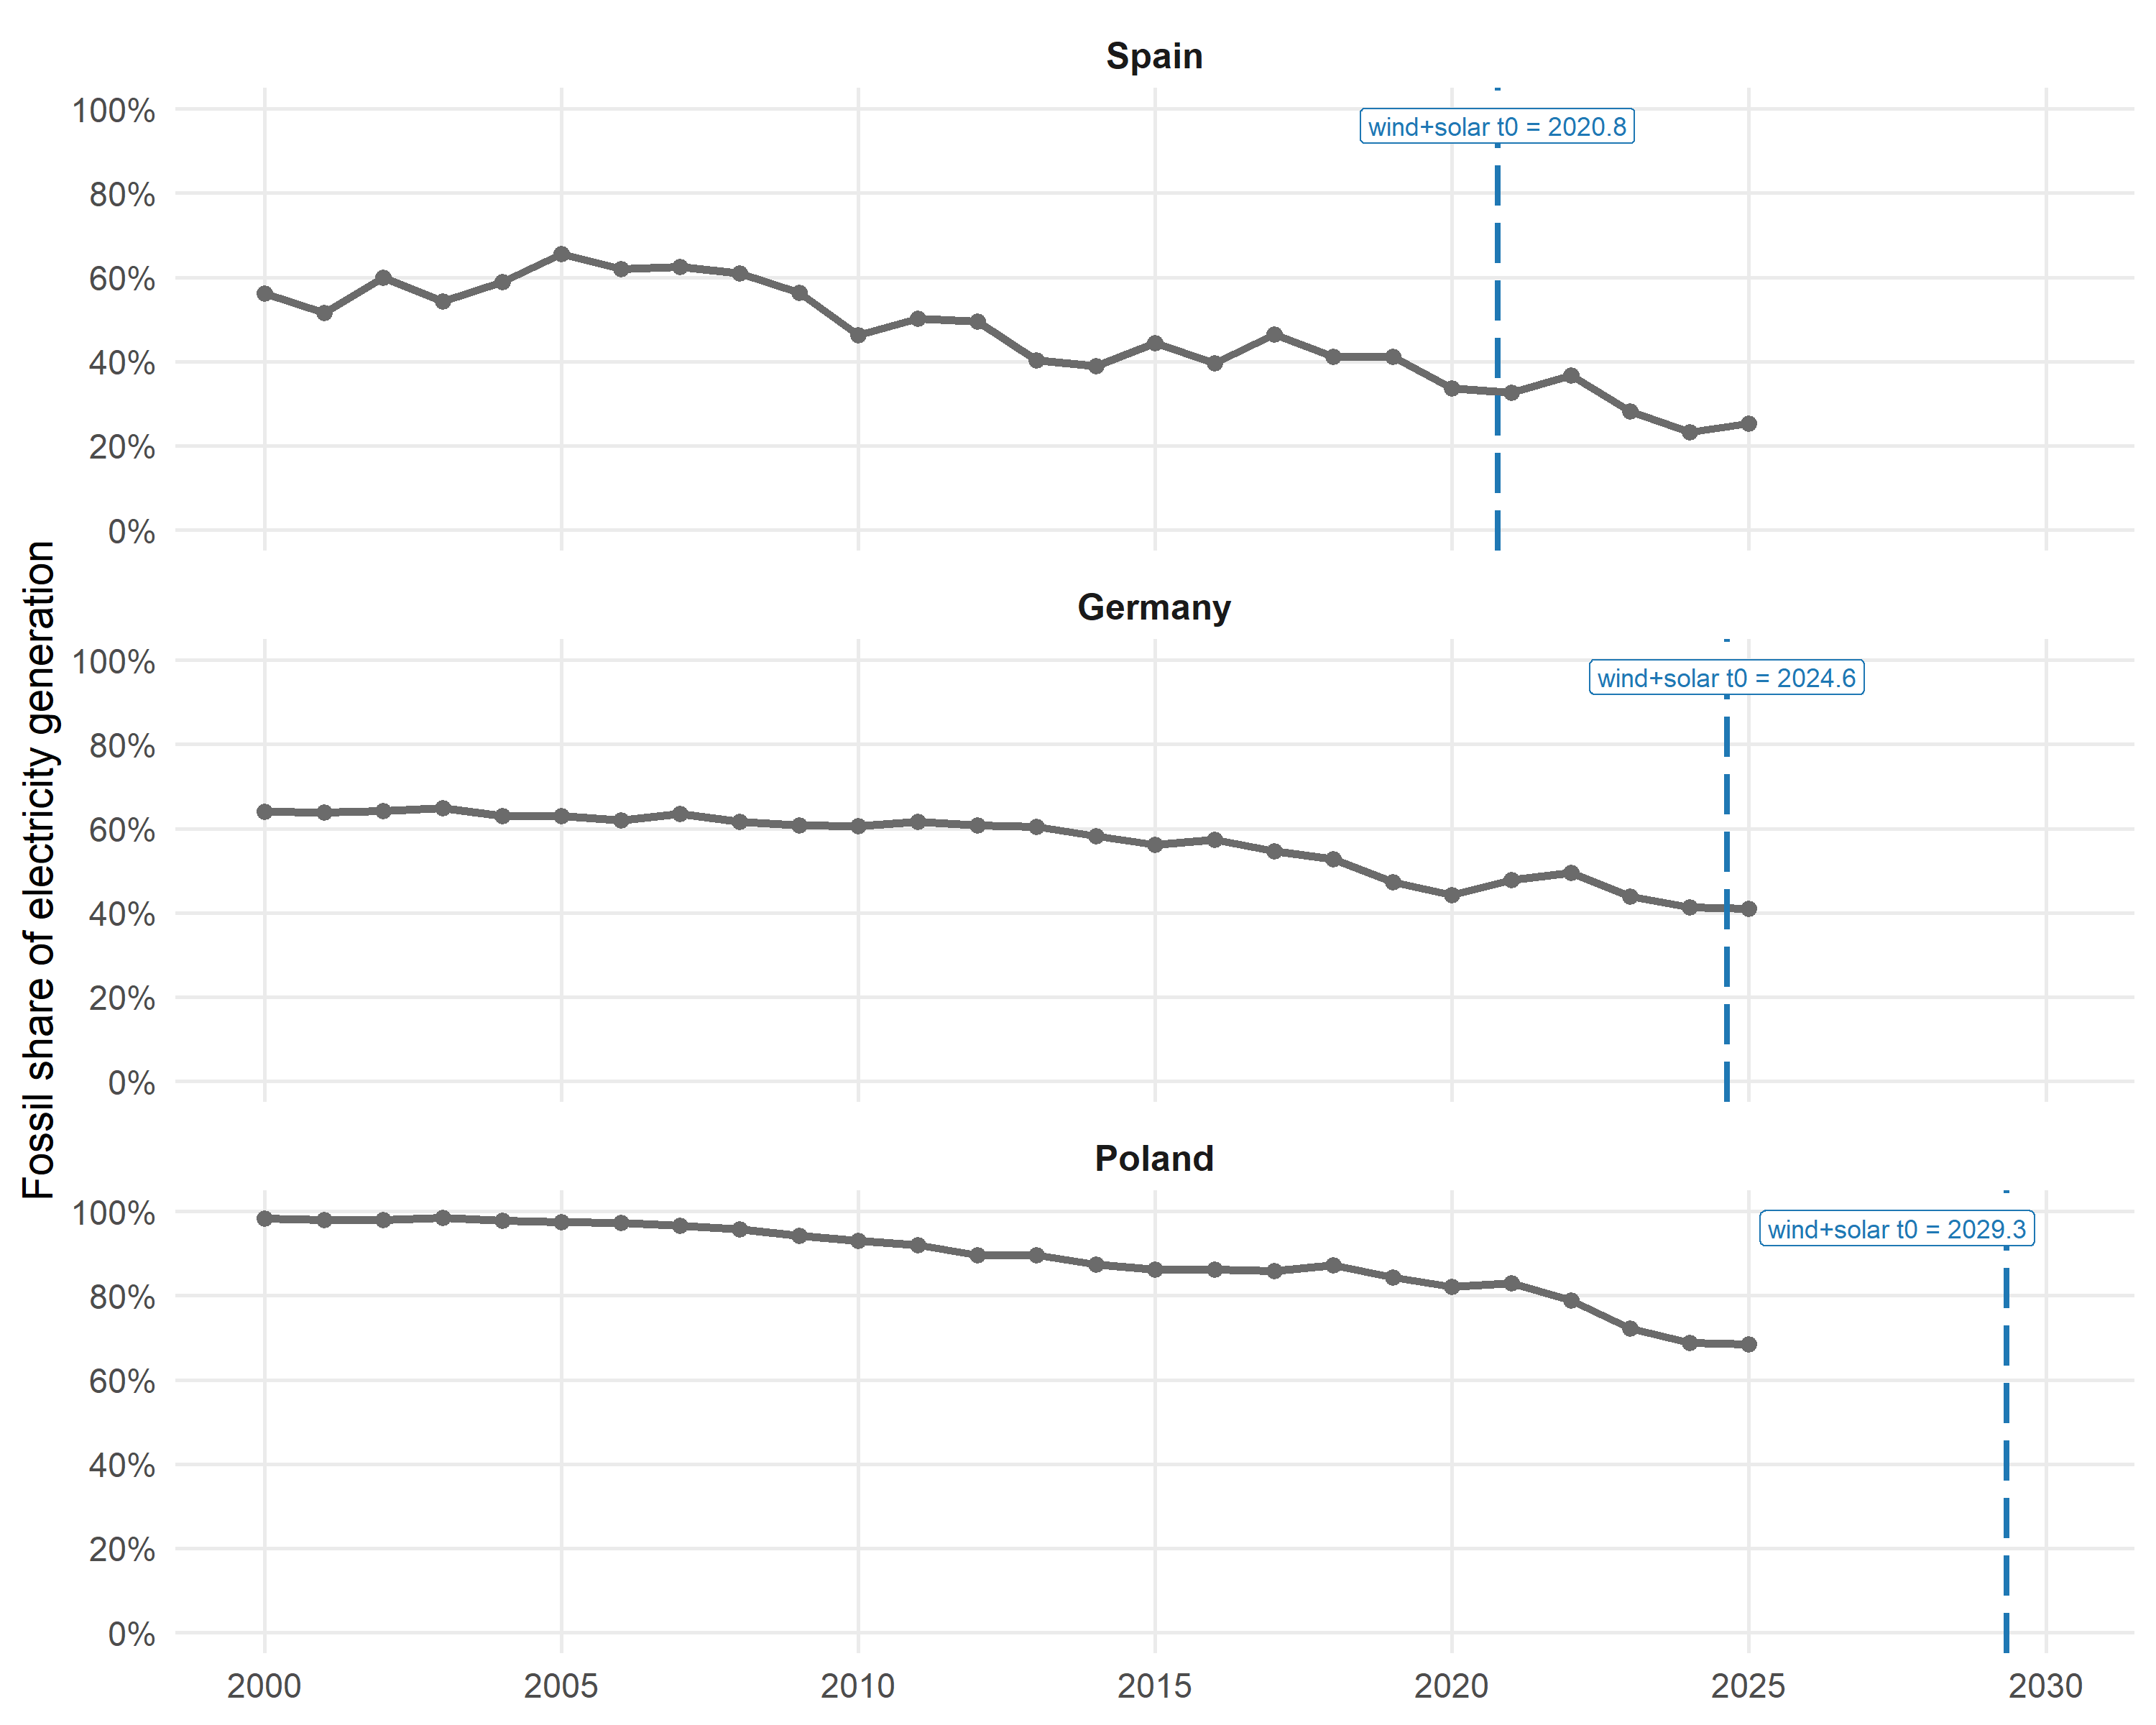
\includegraphics[width=0.9\linewidth]{work/11-positive_tp/figures/fossil_context} 

}

\caption{Aggregate fossil electricity shares and fitted wind and solar inflection years in Spain, Germany and Poland.}\label{fig:ptp-fossilcontext}
\end{figure}

Spain's fossil share falls from around 60 percent to below 30 percent and its renewable inflection occurs during this wider decline. Germany's fossil share falls more clearly after 2015. Its renewable inflection occurs close to parity between the wind and solar share and the fossil share. Poland's fossil share also declines rapidly in the later years although it remains close to 70 percent in 2025.

The projected Polish renewable inflection occurs after the observed fossil series. All three countries therefore show renewable growth alongside fossil decline but they remain at different stages of the transition.

\subsection*{Early warning signals}\label{early-warning-signals}


\subsubsection*{Autocorrelation}\label{autocorrelation}


\begin{figure}

{\centering 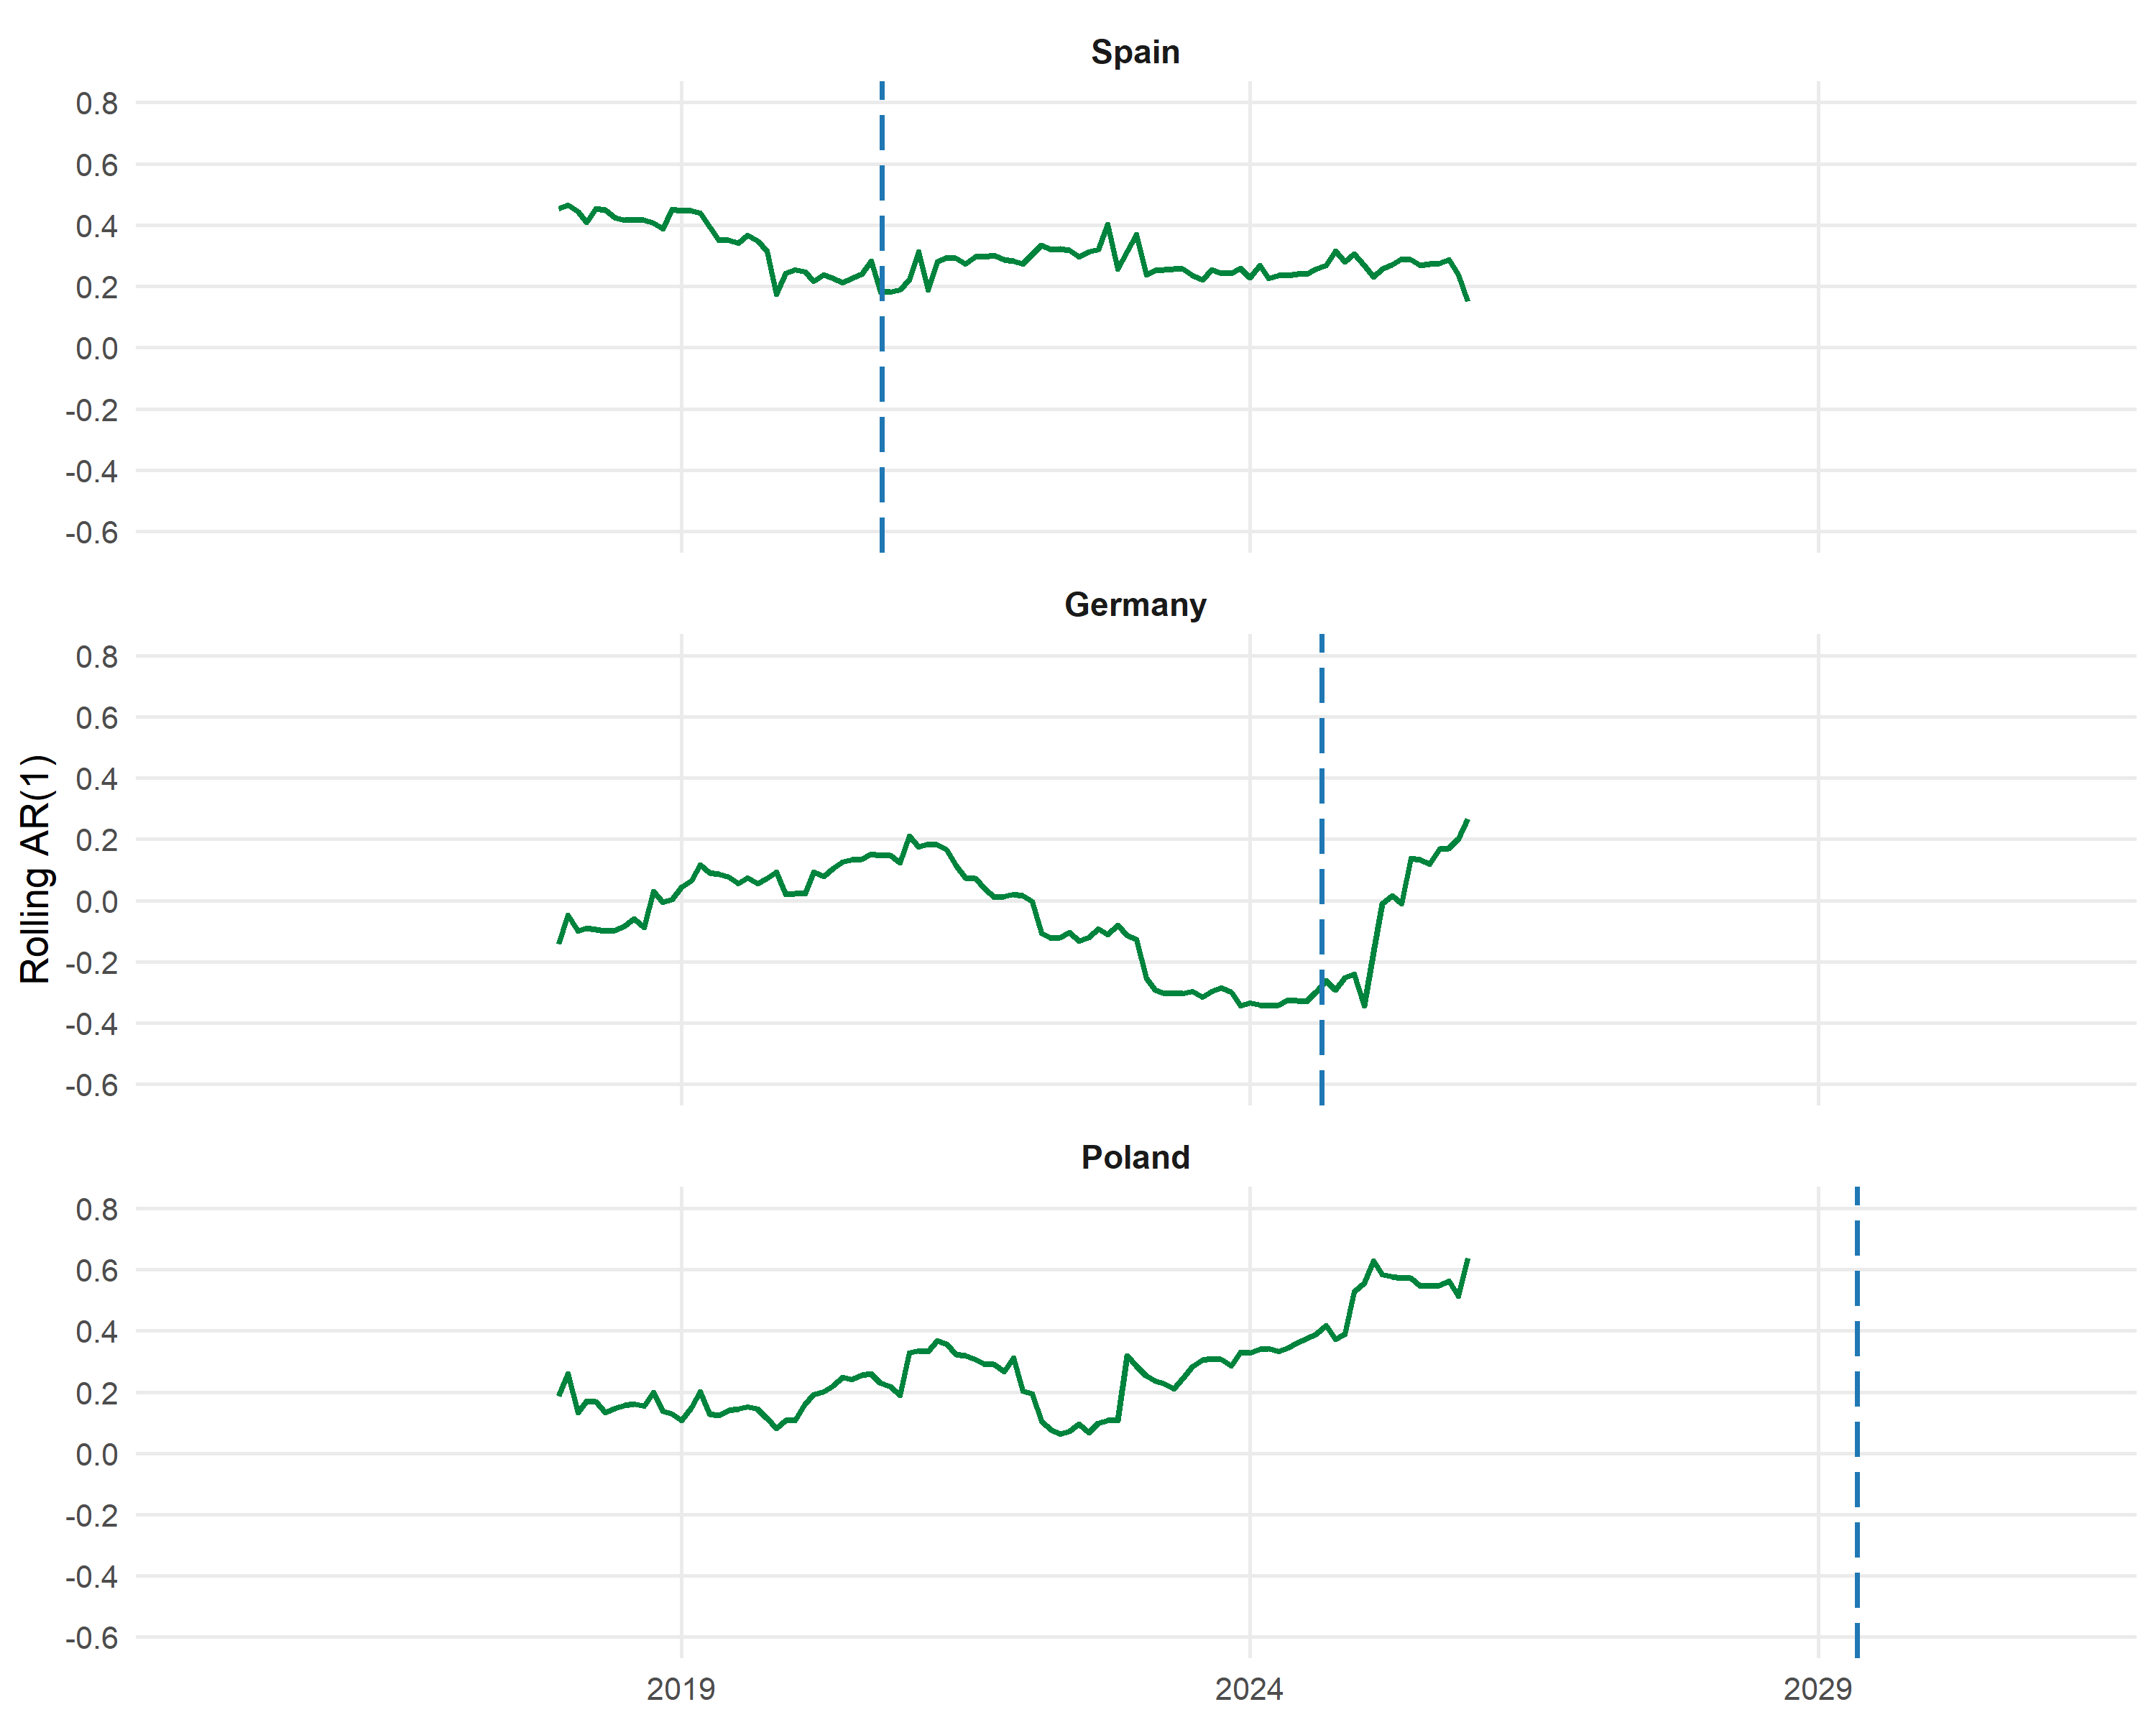
\includegraphics[width=0.9\linewidth]{work/11-positive_tp/figures/ews_ar} 

}

\caption{Rolling lag one autocorrelation of monthly fossil-share residuals. Vertical blue lines indicate the fitted wind and solar inflection dates.}\label{fig:ptp-ewsar}
\end{figure}

Spain does not show a sustained rise in autocorrelation, and its final value of 0.151 is below the valid-window mean of 0.298. Germany shows a recent increase and ends at 0.266 compared with a period mean of minus 0.052. Poland shows the highest final autocorrelation at 0.638 while its period mean is 0.271.

\subsubsection*{Variance}\label{variance}


\begin{figure}

{\centering 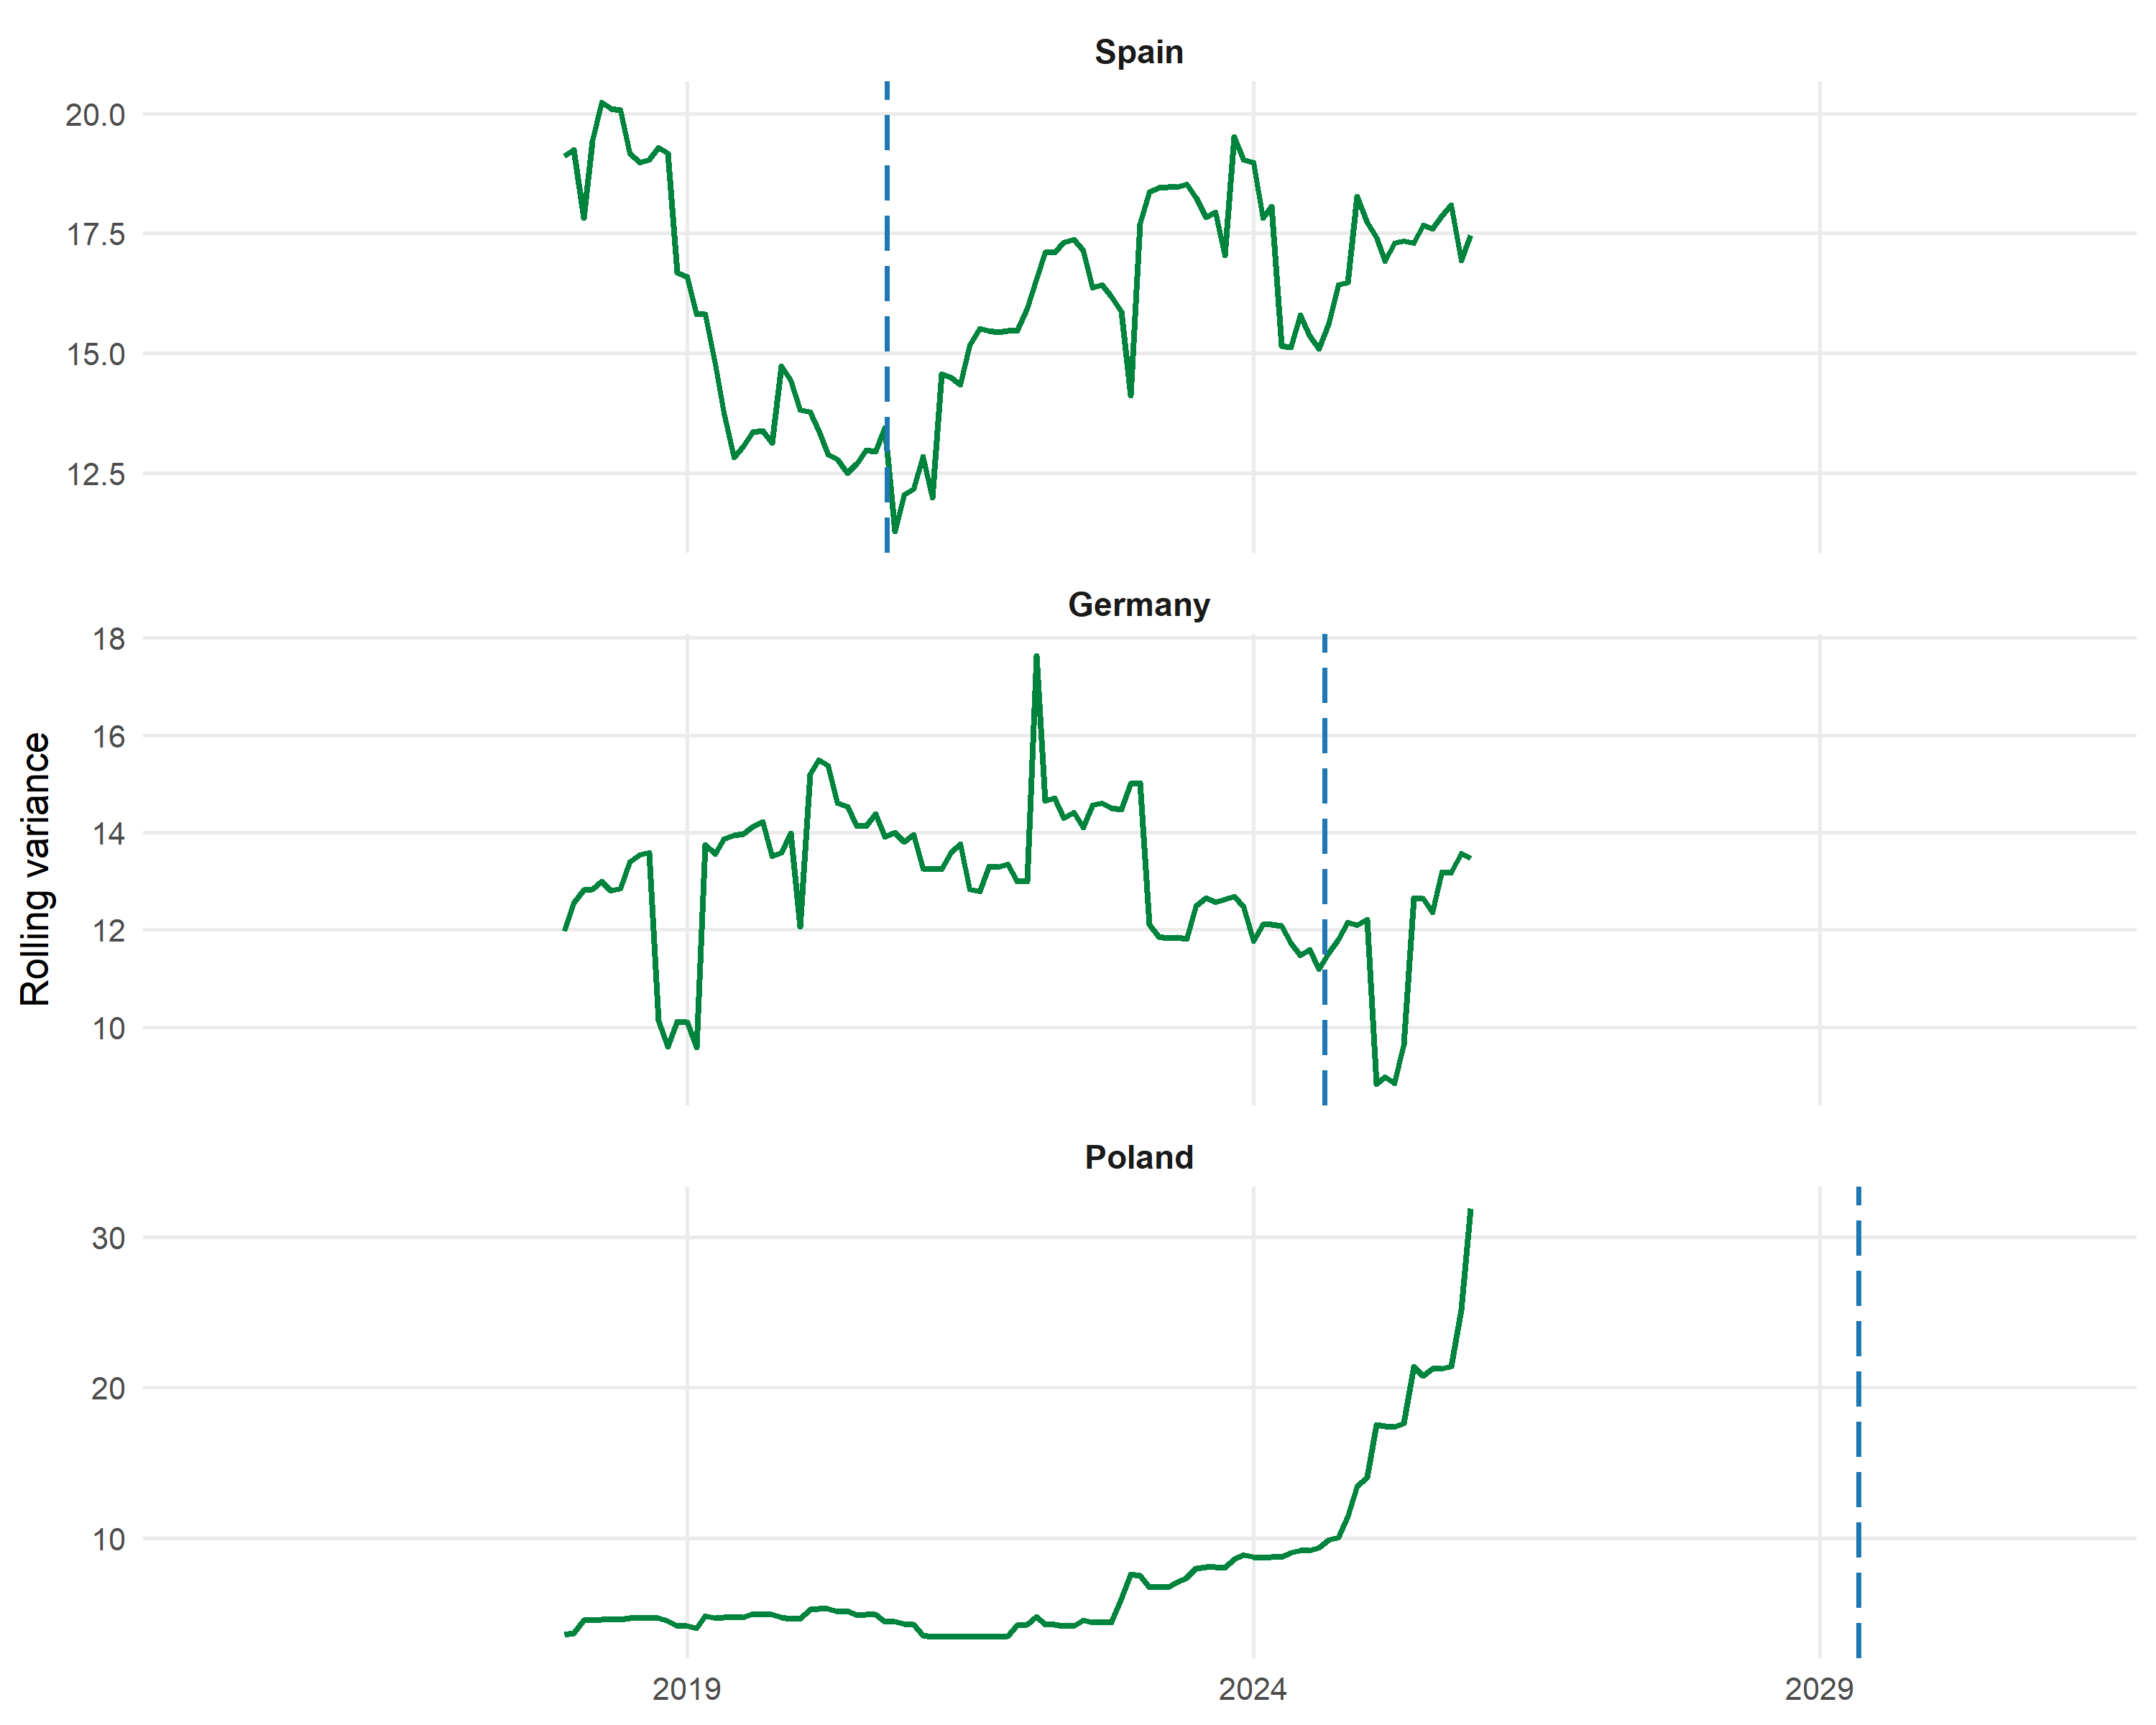
\includegraphics[width=0.9\linewidth]{work/11-positive_tp/figures/ews_variance} 

}

\caption{Rolling variance of monthly fossil-share residuals. Vertical blue lines indicate the fitted wind and solar inflection dates.}\label{fig:ptp-ewsvariance}
\end{figure}

Spain's final variance is 17.5 compared with a period mean of 16.2. Germany ends at 13.5 compared with a mean of 12.9. Poland shows a much stronger increase. Its final variance reaches 31.9 while the period mean is 7.5.

\begin{table}

\caption{\label{tab:ptp-ewssummary}Summary of rolling early warning indicators.}
\centering
\begin{tabular}[t]{l|l|r|r|r|r}
\hline
Country & Indicator & Selected K & Selected t0 & Period mean & Final value\\
\hline
Spain & Rolling AR(1) & 67 & 2021 & 0.298 & 0.151\\
\hline
Spain & Rolling variance & 67 & 2021 & 16.208 & 17.467\\
\hline
Germany & Rolling AR(1) & 88 & 2025 & -0.052 & 0.266\\
\hline
Germany & Rolling variance & 88 & 2025 & 12.946 & 13.463\\
\hline
Poland & Rolling AR(1) & 90 & 2029 & 0.271 & 0.638\\
\hline
Poland & Rolling variance & 90 & 2029 & 7.501 & 31.914\\
\hline
\end{tabular}
\end{table}

The Polish series shows the clearest joint increase in autocorrelation and variance. Germany shows a smaller change while Spain remains comparatively stable.

\section*{Discussion}\label{discussion-3}


The three countries show S shaped wind and solar paths at different stages. Spain appears to have passed its fitted inflection, Germany reaches it near the end of the sample and Poland remains before its projected inflection. The results therefore do not suggest one common European transition date.

The fossil share declines as the wind and solar share expands, including a rapid recent fall in Poland despite its continued fossil dependence. Demand, cross border trade and changes in nuclear or hydropower may also affect these shares. The comparison is therefore descriptive rather than causal.

Uncertainty remains. Poland reaches the upper limit of the saturation grid and each annual series contains only 26 observations. The bootstrap bands cover uncertainty within the selected logistic model, not alternative model families. Denmark and the United Kingdom are contextual benchmarks rather than a formal comparison group.

\section*{Conclusion}\label{conclusion-4}


Denmark and the United Kingdom illustrate two advanced transition paths: long renewable expansion in Denmark and rapid coal decline in the United Kingdom. Both show how a new system can grow while the incumbent weakens.

Spain represents an observed inflection case and its wind and solar share has overtaken the fossil share. Germany's fitted inflection lies close to 2025. Poland shows rapid renewable growth, but its inflection remains projected and fossil electricity still dominates.

Renewable growth occurs alongside declining fossil shares in all three countries. The early warning evidence is less uniform: Poland shows the strongest increases, Germany shows partial evidence and Spain little movement. These indicators remain exploratory and do not provide a common signal.

Overall, the results are more consistent with accelerating renewable diffusion than with one directly observed tipping threshold. Spain appears more advanced, Germany is near its fitted inflection and Poland remains at an earlier stage despite rapid recent change. Positive tipping is therefore better understood as a process than one universal date. Future trajectories may differ because the projections depend on the fitted model and current conditions.

\chapter{Graphics and communication of risks by tipping points}\label{ctp}

\emph{Author: }

\emph{Supervisor: Helmut Küchenhoff}

\emph{Degree: Bachelor/Master}

\section{Abstract}\label{abstract-9}

Lorem ipsum dolor sit amet, consectetur adipiscing elit. Sed do eiusmod tempor incididunt ut labore et dolore magna aliqua. Ut enim ad minim veniam, quis nostrud exercitation ullamco laboris nisi ut aliquip ex ea commodo consequat. Duis aute irure dolor in reprehenderit in voluptate velit esse cillum dolore eu fugiat nulla pariatur. Excepteur sint occaecat cupidatat non proident, sunt in culpa qui officia deserunt mollit anim id est laborum.

\section{Introduction}\label{introduction-10}

\bibliography{nh-bib.bib,ptp-bib.bib,unc-bib.bib,tp-book.bib,dp-bib.bib,book.bib,rh-bib.bib,packages.bib}

\backmatter
\printindex

\end{document}
